% crystal2-a11y.tex -- ACCESSIBILITY SMOKE TEST: front matter + ONE chapter (knn1).
%
% Build with pdfLaTeX on TeX Live 2026 (or LaTeX 2025-11-01+):
%   pdflatex crystal2-a11y.tex
%   makeindex crystal2-a11y.idx      (optional for the test)
%   pdflatex crystal2-a11y.tex
% or just:  latexmk -pdf crystal2-a11y.tex
%
% After compiling, grep the .log for "tagpdf" warnings before uploading to Canvas.
%
% \DocumentMetadata MUST be the very first thing in the file (before
% \documentclass) and may only appear once.
\DocumentMetadata{
  lang        = en-US,
  pdfstandard = ua-2,     % PDF 2.0 + PDF/UA-2: the tagging project's primary target
  tagging     = on,
  % If Ally reports the file as untagged / heading-less even though it isn't,
  % swap the pdfstandard line above for these two (PDF 1.7 + PDF/UA-1):
  % pdfversion  = 1.7,
  % pdfstandard = ua-1,
}

\documentclass[11pt]{book}   % was memoir, which is currently-incompatible with tagging

% -----------------------------------------------------------------------------
% Page layout -- replaces memoir's \setstocksize ... \checkandfixthelayout block.
% These values were measured from memoir itself with the book's layout commands,
% so the typeblock matches the print edition exactly (317pt x 514.2pt, spine
% margin 82.47pt, fore-edge 1.2cm, upper margin 80pt, headsep 16.4pt).
% The online build uses the trimmed 6in x 9in page; for a Blurb print build add
% paperwidth=6.125in, paperheight=9.25in and geometry's layout* keys for the
% .125in trims.
% -----------------------------------------------------------------------------
\usepackage[paperwidth=6in, paperheight=9in,
            textwidth=317pt, textheight=514.2pt, outer=34.14pt, top=80pt,
            headheight=13.6pt, headsep=16.4pt, footskip=27.46pt]{geometry}

% -----------------------------------------------------------------------------
% Packages kept -- all listed as compatible or partially-compatible with tagging.
% -----------------------------------------------------------------------------
\usepackage[svgnames,dvipsnames]{xcolor}   % replaces color + xcolor; AliceBlue is from svgnames
\usepackage{array}
\usepackage{multicol}
\usepackage[T1]{fontenc}
\usepackage{makeidx}
\usepackage{fancyvrb}
\usepackage{dingbat}     % \leftthumbsup / \leftthumbsdown item labels (spyder, datesTimes, longWideTidy).
                         % MUST come before amssymb/MnSymbol: dingbat \newcommand's \checkmark,
                         % amsfonts only defines it if undefined, MnSymbol overrides silently.
                         % Partially compatible: the glyphs lack ToUnicode, which Ally doesn't check.
\usepackage{amsmath,amsthm,amsfonts,amssymb,latexsym}
\usepackage{MnSymbol}    % OK under pdfLaTeX. Drop it if you ever move to LuaLaTeX + MathML (no luamml support).
\usepackage{upquote}
\usepackage{graphicx}    % \includegraphics[alt={...}] / [artifact] is the alt-text interface
\usepackage[hidelinks]{hyperref}
\hypersetup{
  pdftitle  = {The Crystal Ball Instruction Manual, Volume Two: Foundations for Data Science},
  pdfauthor = {Stephen Davies and Evan Coleman},
  pdfdisplaydoctitle = true,   % viewers show the title instead of the file name
}

% -----------------------------------------------------------------------------
% Removed from the original preamble
%   Incompatible with tagging and used nowhere in the book:
%     ulem wrapfig float fancybox varwidth vwcol changepage afterpage footnote
%     (+ \makesavenoteenv) epsfig refstyle makecell longtable textcomp enumitem
%   Partially compatible (missing ToUnicode) but used nowhere in the book:
%     bbding wasysym aurical
%   Incompatible and dropped -- captions revert to the class default look:
%     caption
%   Replaced below: paralist (compactitem/compactenum), the \FV@BeginVBox
%     "bgcolor" hack (ShadedCode), framed's shaded (commented tcolorbox shim)
%   \VerbatimFootnotes: exactly one footnote in the book (synthetic2.tex) has
%     verbatim material in it -- rewrite that one instead.
%   \bluebox / \ignorept / custommargins: unused.
% -----------------------------------------------------------------------------

% ---- paralist replacement: 40 compactitem + 13 compactenum, none with optional args.
% The tight spacing is lost for now: the kernel's new list code documents start=
% and resume= but not (yet) enumitem's nosep/itemsep keys. Restore compactness
% later with the classic \itemsep/\parsep/\topsep lengths.
\NewDocumentEnvironment{compactitem}{}{\begin{itemize}}{\end{itemize}}
\NewDocumentEnvironment{compactenum}{}{\begin{enumerate}}{\end{enumerate}}

% ---- Table helpers. Macros rather than raw \tagpdfsetup so the same chapter
% source also compiles under the old memoir/print preamble -- add there:
%   \providecommand{\HeaderRows}[1]{} \providecommand{\HeaderCols}[1]{}
%   \providecommand{\HeaderRowsCols}[2]{} \providecommand{\LayoutTable}{}
%   and the ShadedCode / ShadedCodeFn environments defined further down
% The tagging code's table settings are STICKY (they apply to every later table
% until changed), so each macro sets all three keys explicitly and every table
% gets exactly one of these immediately before it.
\newcommand{\HeaderRows}[1]{\tagpdfsetup{table/tagging=true, table/header-rows={#1}, table/header-columns={}}}
\newcommand{\HeaderCols}[1]{\tagpdfsetup{table/tagging=true, table/header-rows={}, table/header-columns={#1}}}
\newcommand{\HeaderRowsCols}[2]{\tagpdfsetup{table/tagging=true, table/header-rows={#1}, table/header-columns={#2}}}
\newcommand{\LayoutTable}{\tagpdfsetup{table/tagging=false}}             % alignment-only table:
%   no table structure at all, content tagged as running text. (Not
%   'presentation': that keeps a Table structure with an ARIA role, and math
%   cells then open their Formula before the cell's TD -> invalid nesting.)

% ---- Replacement for the BVerbatim "bgcolor=AliceBlue" blocks (10, all in
% databases.tex). bgcolor= is NOT a fancyvrb key: the print preamble creates it
% by redefining fancyvrb's box internals (\FV@BeginVBox / \FV@EndVBox) to wrap
% the finished box in a \colorbox. That patch would silently override whatever
% the tagging code does to the same internals, so here the same picture is
% built from public API only: BVerbatim in an lrbox, then \colorbox. (frame=
% and framesep= on the originals never did anything -- fancyvrb draws frames
% for Verbatim only -- so the look is identical: blue fill, no rule.)
% Two argument-free environments: an optional argument would swallow the line
% end that BVerbatim needs, so the font size is baked into the name.
% Print preamble: the same two definitions work there unchanged (they need
% only fancyvrb and xcolor's svgnames), so add them alongside the bgcolor hack.
\newsavebox{\CBcodebox}
\newenvironment{ShadedCode}
  {\VerbatimEnvironment\begin{lrbox}{\CBcodebox}\begin{BVerbatim}[fontsize=\small]}
  {\end{BVerbatim}\end{lrbox}\noindent\colorbox{AliceBlue}{\usebox{\CBcodebox}}}
\newenvironment{ShadedCodeFn}
  {\VerbatimEnvironment\begin{lrbox}{\CBcodebox}\begin{BVerbatim}[fontsize=\footnotesize]}
  {\end{BVerbatim}\end{lrbox}\noindent\colorbox{AliceBlue}{\usebox{\CBcodebox}}}

% ---- framed's "shaded" (3 uses: longWideTidy.tex, featureSelection.tex).
% framed is incompatible with tagging, so the box is drawn with tcolorbox.
% tcolorbox >= 6.9.0 tags basic boxes itself (6.10.0 also fixed
% \newtcolorbox-defined boxes, tagging-project #1114); Overleaf's TeX Live 2026
% image has 6.10.0, so a plain wrapper is all that is needed. Two rules for the
% chapters: each use must be preceded and followed by a blank line, and a list
% inside the box should be a native enumerate/itemize, not compactenum/
% compactitem -- the wrapper environments below add a group boundary that
% interferes with the kernel's end-of-list handling when the list is the last
% thing in a box.
\usepackage{tcolorbox}
\providecolor{shadecolor}{rgb}{.84,.84,1}
\NewDocumentEnvironment{shaded}{}
  {\begin{tcolorbox}[colback=shadecolor, colframe=shadecolor, boxrule=0pt,
                     sharp corners, left=2pt, right=2pt, top=2pt, bottom=2pt]}
  {\end{tcolorbox}}
% For a tcolorbox older than 6.9.0 (TeX Live 2025 images), replace the
% definition above with this one, which does by hand what 6.9.0+ does itself:
% neutralise the kernel's minipage plugs around the box and mark the
% background drawing as an artifact. Never switch paragraph tagging off inside
% the environment: the content's closing \par must run with tagging on.
%\ExplSyntaxOn
%\NewDocumentEnvironment{shaded}{}
%  {
%    \cs_if_exist:NT \socket_if_exist:nT
%      { \socket_if_exist:nT { tagsupport/minipage/before }
%          { \AssignTaggingSocketPlug{minipage/before}{noop}
%            \AssignTaggingSocketPlug{minipage/after}{noop} } }
%    \pgfkeysifdefined{/tikz/artifact/.@cmd}
%      { \tikzset{every~picture/.append~style={artifact}} } {}
%    \begin{tcolorbox}[colback=shadecolor, colframe=shadecolor, boxrule=0pt,
%                      sharp~corners, left=2pt, right=2pt, top=2pt, bottom=2pt]
%  }
%  { \end{tcolorbox} }
%\ExplSyntaxOff
% FALLBACK if the Parent-Child warnings still appear at the box: no tcolorbox
% at all -- the kernel's own \colorbox + \parbox, used the way the minipage
% tagging expects them (inside a paragraph). Comment out the definition above
% and uncomment this one. (Body is grabbed as an argument: fine for these three
% boxes, which contain only text and lists.)
%\NewDocumentEnvironment{shaded}{+b}
%  {\par\noindent\colorbox{shadecolor}{\parbox{\dimexpr\linewidth-2\fboxsep\relax}{#1}}\par}
%  {}

\definecolor{darkgreen}{rgb}{0,.55,0}   % defined but unused in the chapters; harmless
\definecolor{darkred}{rgb}{.75,0,0}

\makeindex

\setlength{\parindent}{0pt}
\setlength{\parskip}{6pt}

\begin{document}

\title{{\huge The Crystal Ball Instruction Manual}\\{\large Volume Two:
Foundations for Data Science}\\
{\small version 1.5 -- accessibility test build}}
\author{Stephen Davies, Ph.D., and Evan Coleman, Ph.D.\\Computer Science Department\\University of Mary Washington}
\date{}
\maketitle

\thispagestyle{empty}

Copyright \textcopyright \ 2020 Stephen Davies.

\bigskip

University of Mary Washington\\
Department of Computer Science\\
James Farmer Hall B22\\
1301 College Avenue\\
Fredericksburg, VA  22401

\vspace{.4in}

Permission is granted to copy, distribute, transmit and adapt this work under a
Creative Commons Attribution-ShareAlike 4.0 International License:

\vspace{-.2in}
\begin{center}

\includegraphics[alt={Creative Commons Attribution-ShareAlike 4.0 International license badge}]{cc_license.png}\\
\smallskip
\url{http://creativecommons.org/licenses/by-sa/4.0/}
\end{center}

\vspace{.1in}
If you are interested in distributing a commercial version of this work, please
contact the author at \texttt{stephen@umw.edu}.

\vspace{1.6in}
The \LaTeX source for this book is available from:
\url{https://github.com/rockladyeagles/crystal-ball-2}.

\vspace{.4in}
Cover art copyright \textcopyright \ 2020 Elizabeth M.~Davies.
\frontmatter

\renewcommand{\contentsname}{Contents}
\setcounter{tocdepth}{0}
\tableofcontents

\mainmatter


\chapter{Intermission and review}

Welcome to Volume Two of the Crystal Ball series: \textit{Foundations for Data
Science}! I titled the first volume ``\textit{Introduction to Data Science}''
because it led you through a dip-your-toes-in-the-water experience. You took a
brief tour through the various elements in this diverse field and got a feel
for what it was all about.

Since you're still reading, this means you're still interested, and ready to
explore the next level. In \textit{Foundations}, we'll solidify your growing
knowledge so that you have a firm base on which to build everything else.
Future volumes in this series will cover applications, advanced techniques, and
some special data types that require special treatment. But it all ultimately
rests on the skill set you'll have built in Volumes One and Two of this series.

We're going to dive right in. But first, let me make a list of some of the
things I'm counting on you being pretty solid on:

\begin{compactitem}
\small
\itemsep.1em
\item Atomic and aggregate variables

\begin{compactitem}
\item \texttt{int}s, \texttt{float}s, \texttt{strings}
\item NumPy \texttt{array}s, Pandas \texttt{Series}es, \texttt{DataFrame}s
\item What all these look like in memory
\end{compactitem}

\item Scales of measure (especially categorical vs.~numeric)

\item Assocation vs.~causality

\begin{compactitem}
\item Causal diagrams
\item Dependent and independent variables
\item Observational studies vs.~controlled experiments
\item Confounding factors
\end{compactitem}

\item Statistical significance

\item Exploratory Data Analysis
\vspace{-.18in}
\begin{multicols}{2}
    \begin{compactitem}
    \item Bar charts
    \item Histograms
    \item Contingency tables
    \item Scatterplots
    \item Boxplots
    \item Quantiles
    \item Outliers
    \end{compactitem}
\end{multicols}
\vspace{-.18in}

\item Python stuff
    \begin{compactitem}
    \item Creating and performing calculations on atomic data
    \item Creating and accessing NumPy arrays
    \item \texttt{for} loops
    \item \texttt{if} statements (and \texttt{if}/\texttt{elif}/\texttt{else})
    \item Functions and methods
        \begin{compactitem}
        \item Calling a function/method vs.~writing a function
        \item Passing arguments (both atomic and aggregate)
        \item Return values
        \item Function that modify in-place vs.~returning a copy
        \end{compactitem}

    \item Pandas \texttt{Series} \& \texttt{DataFrames}
        \begin{compactitem}
        \itemsep.1em
        \item Reading from a \texttt{.csv} file
        \item The ``index''
        \item \texttt{.value\_counts()}
        \item \texttt{.groupby()}
        \item Using \texttt{.iloc[]} vs.~\texttt{.loc[]} vs. \texttt{[]}
        \item Single ints/labels vs.~slices vs.~lists
        \item Queries
        \item Recoding / transforming columns
        \end{compactitem}
    \end{compactitem}

\item ML concepts
    \begin{compactitem}
    \item Classification vs.~regression
    \item Features and target attribute
    \item Training data, test data, and new data
    \item Random sampling
    \item The ``prior'' vs.~``posterior''
    \item Evaluating a classifier
    \end{compactitem}

\end{compactitem}

All these topics were covered in \textit{Crystal Ball} Volume One. If any of
them are iffy, you might take an hour or two to flip back through them and
brush up!
           

\chapter{Navigating the Spyder's web}

\index{Spyder}

We'll be using Spyder this semester: a Python-based data analysis environment
written especially for Data Science and scientific programming.

\index{Anaconda}

It comes with the Anaconda distribution, as does pretty much everything else
we'll use this semester (scikit-learn, NumPy, SciPy, Pandas, Matplotlib,
\textit{etc.}) Download it from here: \url{https://www.anaconda.com/download}. 

\textbf{Note:} make sure to get Python \textbf{3.*}, not \textbf{2.*}!! (They
are \textit{not} mutually compatible.) The number(s) after the dot don't
matter so much. But before the dot \textit{must} be a \textbf{``3''}.

\index{Jupyter Notebooks}

Don't worry: all the stuff you learned using Python Jupyter Notebooks still
applies! The only difference is that using an IDE like Spyder is not
Web-based: it's entirely offline, responsive, and more powerful. You will be
creating your own \texttt{.py} files directly.

          

\chapter{EDA: review and extensions}

% contingency table margins
% notched boxplots
% heatmaps
% scatterplot matrices
% facets

\index{Exploratory Data Analysis (EDA)}
\index{univariate}
\index{bivariate}
\index{multivariate}

In this chapter, we'll review the \textbf{EDA} (\textbf{Exploratory Data
Analysis}) material you learned in DATA 101, and also present a few additional
techniques.

Remember, when you're first exploring some data, the first and most basic
questions to ask are:

\begin{compactenum}

\item Is the data \textbf{univariate} or \textbf{bivariate} (or
\textbf{multivariate})?\footnote{``Univariate'' data means that you're looking
at only one variable, even if there are many observations of that variable. A
bunch of people's SAT scores comprises a univariate data set, as does a bunch
of political affiliations, salaries, or declared majors. ``Bivariate'' data
contains \textit{two} pieces of information for \textit{each} observation: if I
have data about both the SAT score and the college GPA for each of a bunch of
students, that's a bivariate data set. Another example: a data set with both
the gender and the salary for each of a bunch of adults.}

\item Is it \textbf{categorical} or \textbf{numerical}?\footnote{Recall that a
``categorical'' variable is qualitative, typically chosen from a set of
possible values. Gender, political affiliation, and declared major are all
examples. ``Numerical'' variables are numbers (duh): salary, GPA, SAT score.
Numerical variables can further be refined by their scale of measure (ordinal,
interval, ratio), although that often doesn't affect the appropriate type of
exploratory statistics and plots too much.}

\end{compactenum}

The answers to these questions determines what kind of \textbf{statistic} is
relevant, and what kind of \textbf{plot} is appropriate.

\pagebreak
Example: let's say we're exploring a data set of great works of literature:

\begin{Verbatim}[fontsize=\small,samepage=true,frame=single,framesep=3mm]
books.iloc[0:5,:]
\end{Verbatim}
\vspace{-.2in}

\begin{Verbatim}[fontsize=\small,samepage=true,frame=leftline,framesep=5mm,framerule=1mm]
                       gender  year     lang   words
name                                                
Jane Eyre                   F  1847  English  183858
The Brothers Karamazov      M  1879  Russian  364153
Anna Karenina               M  1877  Russian  349736
The Inferno                 M  1320  Italian   45750
Huck Finn                   M  1884  English  109571
\end{Verbatim}

For each book, we have the \texttt{gender} of the author, the \texttt{year}
and \texttt{language} in which it was written, and the total number of
\texttt{words} it contains. Clearly \texttt{gender} and \texttt{lang} are
categorical variables, while \texttt{year} and \texttt{words} are numeric.

\section{Case 1: univariate categorical data}
\label{contingencyTable}
\index{contingencyTable}

\index{value\_counts@\texttt{.value\_counts()} (Pandas)}

When looking at just one variable, which is categorical in nature, the
appropriate analysis is the \textbf{one-dimensional contingency table}, which
shows the counts of the various values. Let's create a contingency table for
the book languages, using Pandas' \texttt{.value\_counts()} function:

\begin{Verbatim}[fontsize=\small,samepage=true,frame=single,framesep=3mm]
books['lang'].value_counts()
\end{Verbatim}
\vspace{-.2in}

\begin{Verbatim}[fontsize=\small,samepage=true,frame=leftline,framesep=5mm,framerule=1mm]
French     299
English    247
Spanish    217
Russian    150
Italian     92
Name: lang, dtype: int64
\end{Verbatim}

The most appropriate plot is a \textbf{bar chart} of these counts, which you
can create by simply tacking \texttt{.plot(kind="bar")} at the end:

\begin{Verbatim}[fontsize=\small,samepage=true,frame=single,framesep=3mm]
books['lang'].value_counts().plot(kind="bar")
\end{Verbatim}

\begin{center}
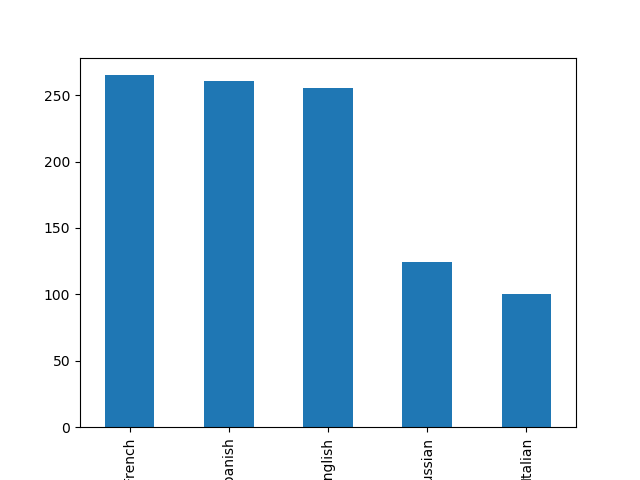
\includegraphics[width=0.6\textwidth]{barplot.png}
\end{center}

\section{Case 2: univariate numeric data}

\index{mean}
\index{standard deviation}
\index{quantiles}

When your single variable of interest is numeric, as is the \texttt{words}
column, the appropriate statistics are \textbf{mean}, \textbf{standard
deviation}, and the various \textbf{quantile} statistics (\textbf{minimum},
\textbf{.25 quantile},  \textbf{median}, \textbf{.75 quantile}, and
\textbf{maximum}):

\begin{Verbatim}[fontsize=\small,samepage=true,frame=single,framesep=3mm]
books['words'].mean()
books['words'].std()
books['words'].quantile([0,.25,.5,.75,1])
\end{Verbatim}
\vspace{-.2in}

\begin{Verbatim}[fontsize=\small,samepage=true,frame=leftline,framesep=5mm,framerule=1mm]
436739.737
232384.719
0.00      5443.0
0.25    241492.0
0.50    462552.0
0.75    637765.0
1.00    805341.0
\end{Verbatim}

Translation: on average, the books in our data set each have about 436,739
words, and if distributed normally (which we haven't checked yet) about
$\frac{2}{3}$rds of them are in the range 436,739 $\pm$ 232,384 (or between
204355 and 669123 words). The shortest book has 5443 words, the longest a
whopping 805,341, and half the books in the data set have 462,552 or less. A
quarter of the books have fewer than 241,492 words, and three quarters have
fewer than 637,765.

\index{histogram}

The best plot in this case is the \textbf{histogram}:

\begin{Verbatim}[fontsize=\small,samepage=true,frame=single,framesep=3mm]
books['words'].plot(kind="hist",bins=30)
\end{Verbatim}

which shows the entire ``lay of the land'' of the distribution of values.
Remember to experiment with the number of \texttt{\textbf{bins}}, since you
can get very different pictures of how the data is distributed depending on
your bin size (more on that in Lesson~\ref{ch:KDEs}).

\begin{center}
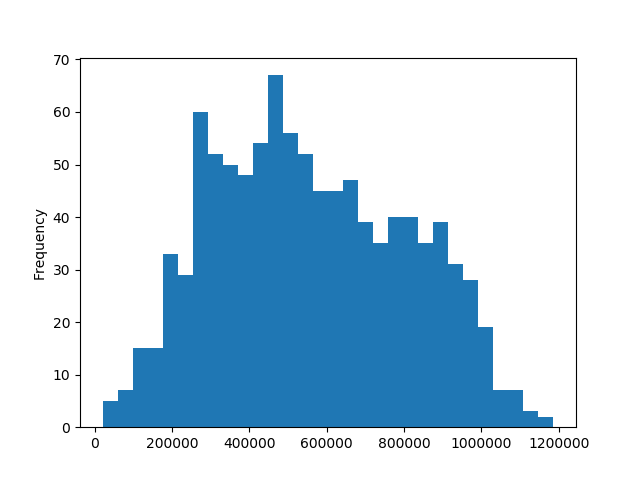
\includegraphics[width=.7\textwidth]{histogram.png}
\end{center}

\section{Case 3: bivariate data: categorical--categorical}

\index{groupby@\texttt{.groupby()} (Pandas)}

If you want to explore the relationship between two different variables, both
of which are categorical, you need a \textbf{two-dimensional contingency
table}. You can use \texttt{.value\_counts()} again in conjunction with
\texttt{.groupby()}):

\begin{Verbatim}[fontsize=\small,samepage=true,frame=single,framesep=3mm]
books.groupby('gender')['lang'].value_counts()
\end{Verbatim}
\vspace{-.2in}

\begin{Verbatim}[fontsize=\small,samepage=true,frame=leftline,framesep=5mm,framerule=1mm]
gender  lang   
F       French      79
        English     52
        Spanish     34
        Italian     29
        Russian     11
M       French     209
        English    196
        Spanish    193
        Russian    115
        Italian     87
Name: lang, dtype: int64
\end{Verbatim}

\index{crosstab@\texttt{.crosstab()} (Pandas)}

which shows, for each \texttt{gender}, how many books in each \texttt{lang} are
in the data set. I personally think the \texttt{pd.crosstab()} function is a
bit easier on the eyes for this, though:

\texttt{gender\_lang@\texttt{gender\_lang}}

\begin{Verbatim}[fontsize=\small,samepage=true,frame=single,framesep=3mm]
gender_lang = pd.crosstab(books['lang'], columns=books['gender'])
print(gender_lang)
\end{Verbatim}
\vspace{-.2in}

\begin{Verbatim}[fontsize=\small,samepage=true,frame=leftline,framesep=5mm,framerule=1mm]
gender    F    M
lang            
English  52  196
French   79  209
Italian  29   87
Russian  11  115
Spanish  34  193
\end{Verbatim}


\subsection{Margins: raw counts}
\label{marginsBegin}
\index{margins (of a contingency table)}
\index{raw counts@``raw'' counts}

\index{crosstab@\texttt{.crosstab()} (Pandas)}

The \texttt{pd.crosstab()} function is also useful for computing
\textbf{margins}, or row/column aggregate information. The easy part is to
include ``\texttt{margins=True}'' as an argument to \texttt{pd.crosstab()}. The
tricky part is understanding the different ways of presenting the margins,
since they're each subtly different and often confused. So heads up. Our first
use of margins will be to simply compute \textbf{raw counts}:

\begin{Verbatim}[fontsize=\footnotesize,samepage=true,frame=single,framesep=3mm]
gender_lang = pd.crosstab(books['lang'], columns=books['gender'], margins=True)
print(gender_lang)
\end{Verbatim}
\vspace{-.2in}

\begin{Verbatim}[fontsize=\small,samepage=true,frame=leftline,framesep=5mm,framerule=1mm]
gender     F    M   All
lang                   
English   52  196   248
French    79  209   288
Italian   29   87   116
Russian   11  115   126
Spanish   34  193   227
All      205  800  1005
\end{Verbatim}

In this table, the margins are \textit{total counts for each row, and for each
column.} Inspect the table and verify this is so: for each row (say,
\texttt{English}) the sum of the \texttt{F} entry (52) and \texttt{M} entry
(196) is equal to the total in the \texttt{All} entry (248). Similarly, the sum
of the entire first column (the \texttt{F}'s for all languages, which are 52,
79, 29, 11, and 34) is equal to the \texttt{All} element of that column (205).
And of course, the sum of the \texttt{All} rows -- or \texttt{All} columns,
same diff -- is the grand total of 1005.

\subsection{Margins: overall percentages}

Now suppose we \textit{divide every value of this table} by the grand total.
(We could literally divide by the number 1005, or divide by
\texttt{gender\_lang.loc[\textquotesingle All\textquotesingle
][\textquotesingle All\textquotesingle ]}, since that's how to programmatically
obtain the value of the bottom-right-hand entry.) This gives us \textbf{overall
proportions}, and if we multiply by 100, \textbf{overall percentages}:

\begin{Verbatim}[fontsize=\small,samepage=true,frame=single,framesep=3mm]
print(gender_lang / gender_lang.loc['All']['All'] * 100)
\end{Verbatim}
\vspace{-.2in}

\begin{Verbatim}[fontsize=\small,samepage=true,frame=leftline,framesep=5mm,framerule=1mm]
gender       F      M     All
lang                         
English   5.17  19.50   24.68
French    7.86  20.80   28.66
Italian   2.89   8.66   11.54
Russian   1.09  11.44   12.54
Spanish   3.38  19.20   22.59
All      20.40  79.60  100.00
\end{Verbatim}

Note carefully how to interpret this result: the sum total of all the table's
entries (except for those in the \texttt{All} row/column) is equal to 100\%.
This tells us that over $\frac{1}{5}$th (20.8\%) of all these books
\textit{were written in French by males}, only about 1\% of the books
\textit{were written in Russian by females}, and so forth.

\subsection{Margins: percentages by column}

By contrast, sometimes it's more helpful to have \textit{each column} add up to
100\%, rather than the entire table adding up to 100\%. You can accomplish this
like so:

\index{div@\texttt{.div() (NumPy)}}

\begin{Verbatim}[fontsize=\small,samepage=true,frame=single,framesep=3mm]
print(gender_lang.div(gender_lang.loc['All'],axis=1) * 100)
\end{Verbatim}
\vspace{-.2in}

\begin{Verbatim}[fontsize=\small,samepage=true,frame=leftline,framesep=5mm,framerule=1mm]
gender        F       M     All
lang                           
English   25.37   24.50   24.68
French    38.54   26.12   28.66
Italian   14.15   10.88   11.54
Russian    5.37   14.37   12.54
Spanish   16.59   24.12   22.59
All      100.00  100.00  100.00
\end{Verbatim}

(For now, the ``\texttt{.div()}'' call, and the ``\texttt{axis=1}'' thing, are
best to just follow verbatim rather than trying to understand what they mean.)

Notice that every \texttt{All} entry at the bottom is now equal to 100.
(The \texttt{All} entries on the right side are \textit{not}.) This view of
things allows us to see the language data \textit{on a per-gender basis}. For
instance, over 38\% \textit{of all the female authors} wrote in French, whereas
only 26\% \textit{of all the males} were in French.

\subsection{Margins: percentages by row}

We can do the corresponding process on a by-row basis by changing our syntax to
this:

\index{div@\texttt{.div() (NumPy)}}

\begin{Verbatim}[fontsize=\small,samepage=true,frame=single,framesep=3mm]
print(gender_lang.div(gender_lang['All'],axis=0) * 100)
\end{Verbatim}
\vspace{-.2in}

\begin{Verbatim}[fontsize=\small,samepage=true,frame=leftline,framesep=5mm,framerule=1mm]
gender       F      M    All
lang                        
English  20.97  79.03  100.0
French   27.43  72.57  100.0
Italian  25.00  75.00  100.0
Russian   8.73  91.27  100.0
Spanish  14.98  85.02  100.0
All      20.40  79.60  100.0
\end{Verbatim}

\underline{Important}: there are \textit{two} changes here from the previous
example, only one of which jumps out at you. The obvious one is that we have
``\texttt{axis=0}'' instead of ``\texttt{axis=1}''. But the one that's easy to
miss is that instead of ``\texttt{gender\_lang.loc[\textquotesingle
All\textquotesingle ]}'' we now have ``\texttt{gender\_lang[\textquotesingle
All\textquotesingle ]}'' (with \textit{no} ``\texttt{.loc}''). If you forget
this part, you'll get nonsense.

If you do it correctly, each \textit{row} (not column) will now sum to 100\%,
which gives us gender data \textit{on a per-language basis}. For example,
we can see that 91.27\% \textit{of the Russian books} were written by
men, but only 75\% \textit{of the Italian ones} were.

\subsection{\textit{Warning!}}

\index{statistical significance}
\index{$\chi ^2$ test}

Now you can stare at these numbers to get a feel for the them, and this is
encouraged. Remember, though, the proper way to test whether there's a
\textbf{statistically significant} relationship between two categorical
variables is to use a $\chi ^2$ test. And that leads me to mention a very
common pitfall.

\index{chi2\_contingency()@\texttt{chi2\_contingency()} (SciPy)}

Recall that when you call \texttt{scipy.stats.chi2\_contingency()}, you pass it
the contingency table. All well and good. But you must remember to pass it
\textit{the original contingency table \textbf{without} margins!} Once you've
started to compute and display margins, it's all too easy to forget that adding
margins \textit{adds a row and a column to the table} (for the ``\texttt{All}''
information) and if you give \texttt{chi2\_contingency()} this extraneous data
it messes up the whole $\chi ^2$ computation.

This is why in all the examples above, I deliberately did \textit{not} store
the ``margined'' version of the table back into the \texttt{gender\_lang}
variable. Instead, I kept only the table of raw counts in the variable, and
simply \textit{printed} the margined version when necessary, a la:

\begin{Verbatim}[fontsize=\small,samepage=true,frame=single,framesep=3mm]
# Correct!
gender_lang = pd.crosstab(books['lang'], columns=books['gender'])
print(gender_lang.div(gender_lang.loc['All'],axis=1) * 100)
scipy.stats.chi2_contingency(gender_lang)
\end{Verbatim}

I've seen plenty of well-intentioned students do this instead:

\begin{Verbatim}[fontsize=\small,samepage=true,frame=single,framesep=3mm]
# WRONG!
gender_lang = pd.crosstab(books['lang'], columns=books['gender']).div(
    gender_lang.loc['All'],axis=1) * 100)
print(gender_lang)
scipy.stats.chi2_contingency(gender_lang)
\end{Verbatim}

which leads to madness.

\subsection{(Not) plotting multiple categorical variables}

\index{mosaic plot}

Finally, what about plots for multiple categorical variables? Unfortunately,
the only plot I really know of for this is called a \textbf{mosaic plot}, and I
think they're so difficult to interpret that I don't really recommend them. Let
me know if you find a good alternative.

\label{marginsEnd}


\section{Case 4: bivariate data: categorical--numerical}

Suppose the two variables you're interested in are one categorical and one
numerical. For instance, maybe you're wondering whether men or women have
contributed more recent literary works, or which languages tend to have longer
longer books. 

\index{box plot}

The right plot here is the \textbf{box plot}, since it allows you to easily
compare groups. For the language vs.~length example:

\begin{Verbatim}[fontsize=\small,samepage=true,frame=single,framesep=3mm]
books.boxplot(column='words', by='lang')
\end{Verbatim}

\begin{center}
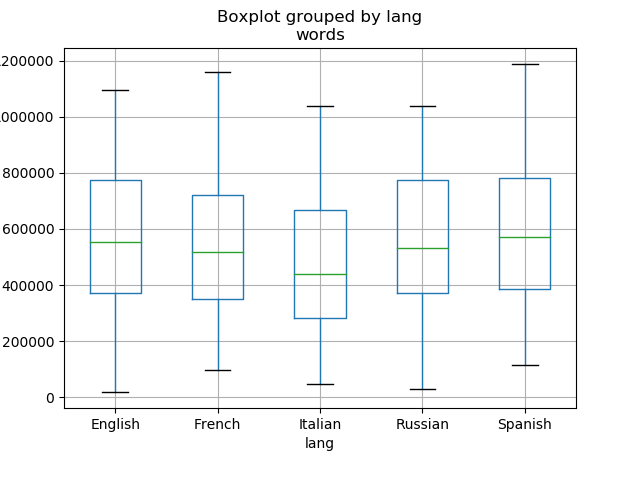
\includegraphics[width=0.8\textwidth]{boxplot.png}
\end{center}

\index{$t$-test}
\index{ttest\_ind@\texttt{ttest\_ind()} (SciPy)}

Apparently Italian works are a bit shorter than the other languages (especially
French), but it's hard to tell whether there's any truly significant difference
between the averages among the various groups. Recall that one way to find this
out is a \textbf{$t$-test for the difference of means}, using
\texttt{scipy.stats.ttest\_ind()}.

\index{box plot!notched}
\index{notched box plot}

Here's another way. You can use a \textbf{\textit{notched} boxplot}:
\label{notched}

\begin{Verbatim}[fontsize=\small,samepage=true,frame=single,framesep=3mm]
books.boxplot(column='words', by='lang', notch=True)
\end{Verbatim}

\index{statistical significance}

As long as your group sizes are big enough, this visually indicates whether or
not there is a stat sig diff between groups, based on \textit{whether the
notched areas overlap}. In the above case, the French and Italian notches
overlap, which means we can conclude \textit{nothing} reliable about French
works being longer than Italian ones. However, the Russian and Italian notches
do \textit{not} have any overlap, which means we \textit{should} feel confident
about declaring that on average, Russian works are longer than Italian ones.

\begin{center}
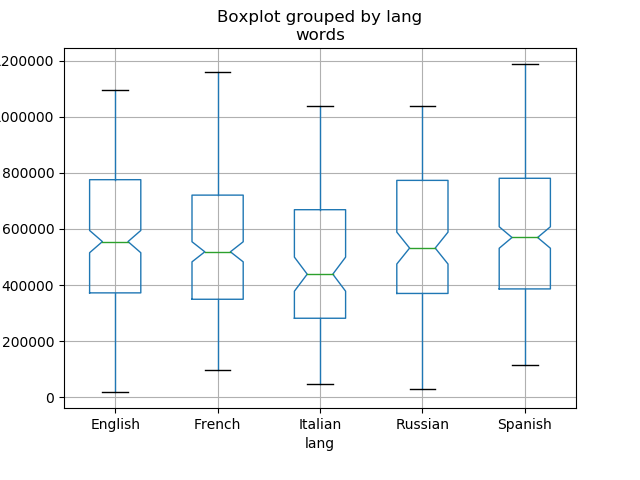
\includegraphics[width=0.9\textwidth]{notchedboxplot.png}
\end{center}

\section{Case 5: bivariate data: numerical--numerical}

\index{scatter plot}

Finally, the case where our two variables of interest are both numerical. The
obvious plot type here is the \textbf{scatter plot}, which shows one point for
each observation, with its $x$ and $y$ position determined by its values for
each variable.

\begin{Verbatim}[fontsize=\small,samepage=true,frame=single,framesep=3mm]
books.plot.scatter(x='year', y='words')
\end{Verbatim}

\index{Pearson correlation coefficient}
\index{correlation coefficient}

Clearly a big takeaway from the scatter plot below is that literary works have
been getting steadily shorter over the years. You'll remember that the
statistical reliability of this conclusion could be confirmed (or denied) by
taking a look at the Pearson's correlation coefficient.

\begin{center}
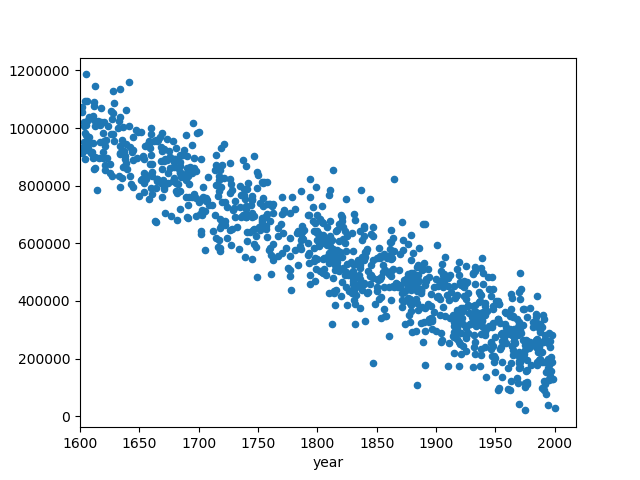
\includegraphics[width=0.9\textwidth]{scatterplot.png}
\end{center}

   

% TODO: do we need to define the word "distribution?!"

\chapter{KDEs and distributions}
\label{ch:KDEs}

\index{histogram}
\section{Limitations of histograms}

Histograms are a great tool for seeing the distribution of a numerical,
univariate sample. As we'll see in this chapter, though, they have some
deficiencies. One problem is that a data set doesn't uniquely determine a
histogram: instead, we must specify parameters such as the bin size and the
``alignment'' of the bins (\textit{i.e.}, where exactly the breaks occur), and
the resulting display is colored (no pun intended) by those choices.

Consider this simple data set\footnote{From Janert, P. K. (2010). Data Analysis
with Open Source Tools: A Hands-On Guide for Programmers and Data Scientists (1
edition). O'Reilly Media.}:

\begin{center}
\texttt{2.1, 2.3, 1.9, 1.8, 1.4, 2.6, 1.7, 2.2}
\end{center}

Suppose we choose a bin width of 1. If we positioned the \textit{left} edge of
each bin at 0, 1, 2, 3, ..., we would get the histogram on the left side of
Figure~\ref{fig:histBinParadox}.

\begin{Verbatim}[fontsize=\footnotesize,samepage=true,frame=single]
data = np.array([2.1, 2.3, 1.9, 1.8, 1.4, 2.6, 1.7, 2.2])
plt.hist(data, bins=[0,1,2,3,4])
\end{Verbatim}

Our interpretation would probably be: ``looks like the values occur pretty
uniformly throughout the range 1-3.''

But if we shifted our bin alignment to be on the ``halves'' (0.5, 1.5, 2.5,
...), we get this histogram on the \textit{right} side of
Figure~\ref{fig:histBinParadox}.

\begin{Verbatim}[fontsize=\footnotesize,samepage=true,frame=single]
plt.hist(data, bins=[-.5,0.5,1.5,2.5,3.5,4.5])
\end{Verbatim}

Now we may be liable to think: ``it looks like a steeply-peaked distribution
with most values right near the center value of 2.''

\smallskip
Yet the data is the \textit{same}! :-O

\begin{figure}[ht]
\centering
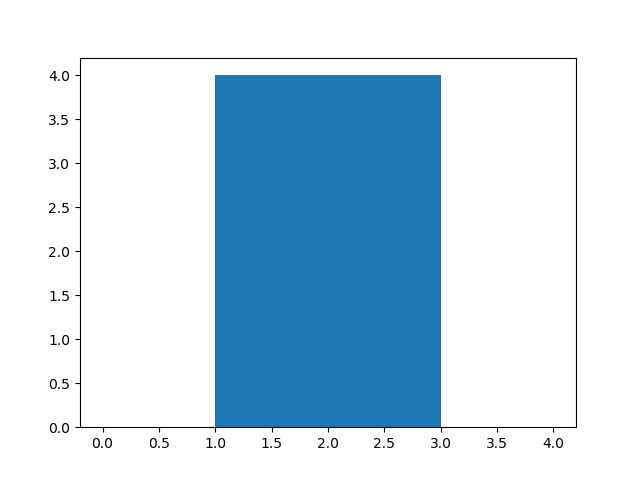
\includegraphics[width=0.45\textwidth]{hist1.png}
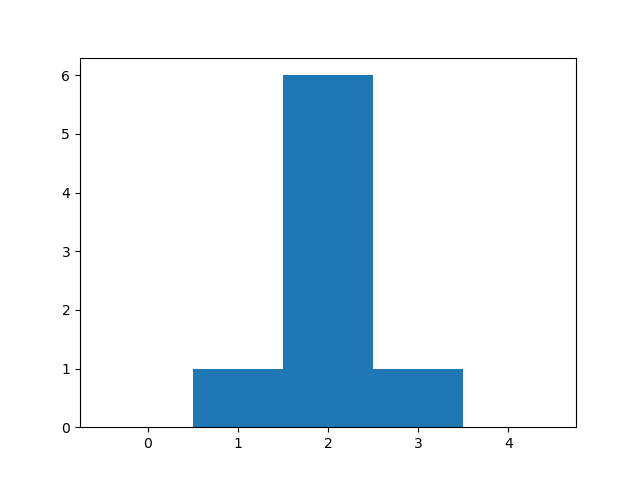
\includegraphics[width=0.45\textwidth]{hist2.png}
\caption{Two histograms of the \textit{same} data set!}
\label{fig:histBinParadox}
\end{figure}
\begin{center}
\end{center}
\vspace{-.6in}

\subsection{Data vs.~process}

Now you might dismiss this idiosyncrasy as merely a one-off quirk that only
shows up when the data is carefully arranged so as to trigger it. And there's
some truth to that. But the real problem with histograms is bigger and more
conceptual: it has to do with \textit{what we're really trying to visualize in
the first place.}

\index{data-generating process (DGP)}

In Data Science, paradoxically, very often we don't actually care about the
\textit{data} so much as we care about the underlying \textit{process} that
generated the data. This ``Data-Generating Process'' (DGP) -- whether it's a
geographic fault, a mystery author, a sports team, or an economy -- leaves
behind evidence of its behavior (seismic tremors, sentences, sports statistics,
income levels) which we dutifully collect and then analyze. The purpose is
(almost) always to draw inferences about how that DGP works, not to learn about
the individual bread crumbs themselves.

To our present point, when we look at a histogram of (say) GPAs of a sample of
UMW students, we're not actually interested in what those sampled GPAs
precisely are, strange as that may sound. We're instead interested in what they
tell us about UMW student GPAs in general. We want to draw conclusions about
the \textbf{population} by looking at the \textbf{sample}.\footnote{If you
haven't encountered these words before, the ``population'' is the entire set of
relevant objects of study that are out there in the world, most of which we'll
never get a direct measurement for because they're just too numerous. The
``sample'' is the small subset of the population that we did get a measurement
for. A classic example is political polling: we don't really care that much how
the 2,000 people in our telephone poll are going to vote for President; what we
care about is how the country as a whole will vote for President. So we assume
that the sample is reflective of the population, and reason accordingly using
statistical tests as our guide.}

Let's say we hung out at the fountain on campus walk, and asked unsuspecting
volunteers to let us measure how tall they were. The histogram of the result
might look like Figure~\ref{kdehist}.

\begin{figure}[ht]
\centering
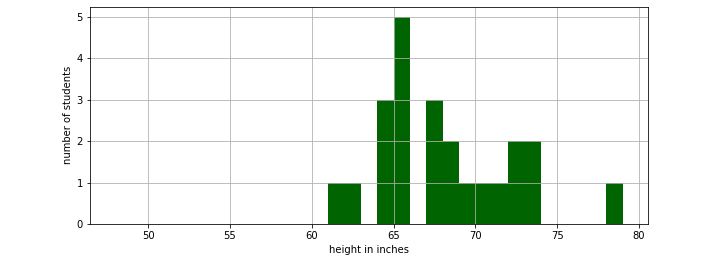
\includegraphics[width=0.7\textwidth]{kdehist.png}
\caption{A histogram of a sample of UMW student heights.}
\label{kdehist}
\end{figure} 

The histogram is using ``1 inch'' as a bin size. By inspecting it, we can see
that the shortest person in our sample was 62 inches tall (or 5-foot-2), the
tallest was 78 inches (6-foot-6), and the most common height was 65 inches
(5-foot-5), among other things.

But consider this. Our sample had five students who were 5-foot-5, three who
were 5-foot-7, but \textit{none} who were 5-foot-6. This is perfectly possible
with samples, of course -- you're only getting a random set of students, and
there are bound to be little quirks like this. But on what basis do we label it
a ``quirk?''

If you're like me, your inclination is to say, ``yeah, okay, in this particular
sample we happened to be missing any 5-foot-6 people, but it's not like we're
going to draw any grand conclusions from that fact. We're not going to deduce
that `UMW students are almost never 5-foot-6 -- they're almost always either a
tad shorter or a tad taller than that.' Such a conclusion would be ludicrous!''

\index{background knowledge}

I sympathize and agree. But really, we only know this because we bring
\textbf{background knowledge} to the problem. We've all seen lots of people of
various heights, and we know something about how genetics and nutrition and
other factors play into a person's height, and it just screams ``wrong!'' to
think that there's some magic ``missing height'' out there, right in the middle
of otherwise quite common heights, that for some reason is virtually
unattainable.

Think about it, though: if we were studying an \textit{unknown} phenomenon,
about which we had no previous experience, it would be pretty audacious for us
to infer the existence of lots of ``66's'' which we never actually observed,
simply on the grounds that there were lots of 65's and 67's in our sample. My
point is not to forsake your background knowledge: quite the opposite, you
should make good use of it! My point is only to draw attention to the
justification we're using to infer the existence of plenty of 66-inch-tall
(5-foot-6) people in the population, even though we never actually observed
any.

So my main point is this. Although we look at a histogram like this one in
order to see ``the lay of the land'' -- to see which values of the numeric
variable are more frequent, and which are less frequent -- if we're smart we
can't help but recognize two different aspects to the figure. Some of the
histogram's features are generalizable, and indicative of what the population
probably looks like: we'd (correctly) gather that many or most UMW students
were between 60 and 80 inches tall, with the majority in the 65-ish to 75-ish
range. But some of its features we'd (correctly) characterize as mere artifacts
of this particular sample, like the weird fact that we happen to have several
65-inchers and 67-inchers but no 66-inchers.

What we'd really like is a plot that obscures (or ``smooths over'') the second
kind of thing, while still revealing the first kind of thing. In other words,
we'd like a plot that shows us the features of the data that are probably
generalizable, while hiding the individual nooks and crannies. Such a plot is
coming right up in Section~\ref{kdes}, below.

Just to finish venting, I'll list yet another couple of problems with
histograms:

\begin{itemize}
\itemsep.1em
\item They inherently lose information, since by definition data points with
specific, precise values are munged into ``the nearest bin.''
\item They don't handle outliers very well. A single outlier way outside the
normal range forces us to either (a) include a lot of empty cells in the
middle, or (b) choose an unreasonably wide bin width that doesn't work for the
majority of points.
\end{itemize}

\section{Kernel Density Estimates (KDEs)}

\label{kdes}

One solution to these unfortunate histogram problems is a more advanced
technique called a \textbf{Kernel Density Estimate}, or a \textbf{KDE}.

\index{kernel}
\index{Gaussian (kernel)}
\index{normal distribution}
\label{Gaussian}

A ``kernel'' is defined as a single, strongly-peaked function that has an area
under its curve of exactly 1. Normally (no pun intended!) we will use a
\textit{Gaussian kernel}, which means ``a bell curve a la the normal
distribution'':

\begin{center}
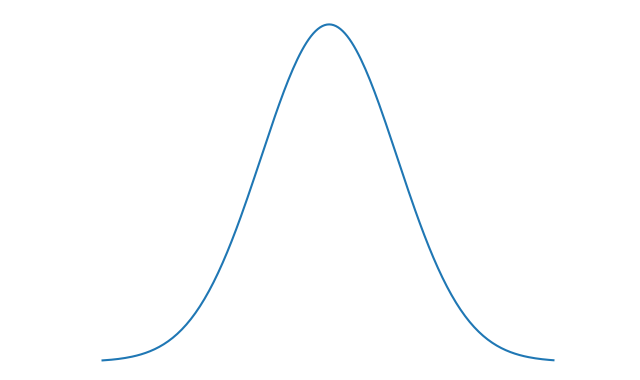
\includegraphics[width=0.4\textwidth]{lilGaussian.png}
\end{center}

(In math and stats, ``Gaussian'' and ``normal'' are synonyms.)

\index{bandwidth}
\index{standard deviation}

One thing we have to decide on is the \textit{width} of this kernel --- which
in our case essentially means ``the standard deviation of the normal
distribution we're using.'' This is kind of like having to choose the bin width
for histograms, but in practice the choice turns out not to be as critical. The
width we choose is called the kernel's \textbf{bandwidth}.

Okay, now visualize this. In order to form a KDE, we place a \textit{copy} of
this kernel on the x-axis at each data point, and then add up all the kernel
contributions to make a smooth curve. This has the effect of smoothing out all
the jaggedy ups and downs of the actual histogram. The goal is to reflect the
``true, underlying'' shape of the data for the entire population.

\index{gaussian\_kde@\texttt{gaussian\_kde()} (SciPy)}
\index{kdeplot@\texttt{kdeplot()} (Seaborn)}

There are several different ways to do this with Python packages. The Seaborn
library has a good ``\texttt{kdeplot()}'' function. Using straight SciPy, we
can call the \texttt{gaussian\_kde()} function and pass it the bandwidth as a
second argument. This returns a function that can be used to evaluate the KDE
at any data point. (Read that sentence again: a function that returns a
function? It can be confusing.) Then, we can plot it by creating a range of
values to evaluate the KDE at, and plotting those values against the KDE's
values.

It's easier than it sounds when you run the actual code:

\index{bw\_method@\texttt{bw\_method} (for \texttt{gaussian\_kde()})}

\begin{Verbatim}[fontsize=\footnotesize,samepage=true,frame=single]
import scipy.stats
kde = scipy.stats.gaussian_kde(data,bw_method=.5)
x_vals = np.arange(0,10,.1)
plt.plot(x_vals,kde(x_vals))
\end{Verbatim}

\index{bandwidth}

The ``\texttt{data}'' argument to \texttt{gaussian\_kde()} is the array you're
working with, and ``\texttt{bw\_method}'' (a dumb name) gives the kernel's
bandwidth. (\texttt{x\_vals} is an array of the x coordinates you want to plot
the KDE for, and should cover the range.)

Now stare at the four plots in Figure~\ref{kdesfig}. These are all KDEs for
the green Figure~\ref{kdehist} histogram, but each one uses a different
bandwidth. Choosing a larger kernel bandwidth effectively smooths out the KDE
more, spreading the contribution of each point quite a bit farther from its
original position. Choosing a narrower kernel focuses each data point's
contribution more precisely at its actual value, making the plot choppier.

\begin{figure}[ht]
\centering
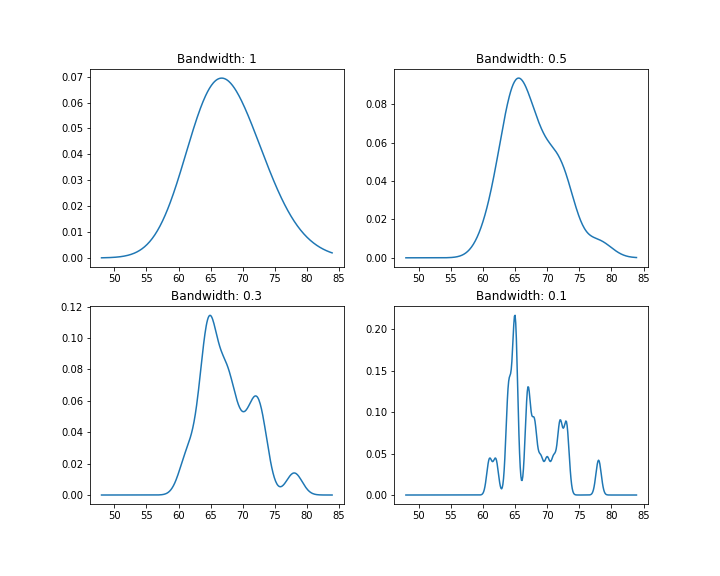
\includegraphics[width=1\textwidth]{kdes.png}
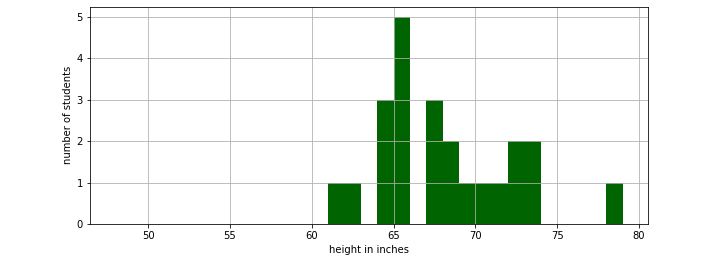
\includegraphics[width=0.7\textwidth]{kdehist.png}
\caption{Gaussian KDEs with bandwidths of 1, .5, .3, and .1, respectively, for
the data behind the green Figure~\ref{kdehist} histogram (repeated here).}
\label{kdesfig}
\end{figure}

In practice, it's another parameter to play with. If the data follows a smooth
distribution, you can use a wider bandwidth which will ``blur'' each data point
more and give a more intuitive view of the general distribution
characteristics. If the distribution is more wiggly, though, you need a
narrower bandwidth to see all the relevant detail. Which of the
Figure~\ref{kdesfig} bandwidths do you think best captures the ``true''
distribution of the points in the histogram?

Like most things in Data Science (and in life), there's no one true
hard-and-fast right answer. There is instead a range of points of view, many
of which may be illuminating.
             

\chapter{Random value generation}

\index{synthetic data set}

One very useful skill is the ability to quickly create \textit{synthetic}
(artificial; generated by your own code and random-number generators) data
sets that have certain properties. Sometimes we use such data to sanity check
the results of our code with ``idealistic'' (simplified and known) inputs.
Sometimes we use synthetic data as a baseline with which to compare real-world
data sets that we suspect have similar characteristics. And sometimes we
simply don't have access to relevant real-world data but we need inputs into
some simulation process.

This chapter and the next will teach you the essentials of this process.

\index{random number}
\index{random value}
\index{seed (of a random generator)}

\section{Setting the seed}

Generating \textbf{random number}s (and other \textbf{random value}s) is an
activity we perform surprisingly often in Data Science. ``Random numbers,'' as
it turns out, aren't truly random, because the programming language uses a
bizarre -- but deterministic and repeatable -- algorithm to come up with them.
This is nice, because we can guarantee that each time we run a program we'll
get the same sequence of random numbers. We do this by setting the random
number generator's \textbf{seed} to a particular value. It helps us in
debugging our code, because otherwise, a shifting sequence of numbers would be
a frustrating moving target. 

\index{seed@\texttt{seed()} (NumPy)}

NumPy provides a really nice library for all this, all of which is in the
namespace \texttt{np.random}. To set the random number generator's seed, all
you do is call its \texttt{seed()} function and pass it your favorite number:

\begin{Verbatim}[fontsize=\small,samepage=true,frame=single,framesep=3mm]
np.random.seed(13)
\end{Verbatim}

(I chose 13 because that was my little league baseball jersey number as a
kid.) I recommend you put this line of code (with any positive integer you
like) near the top of any \texttt{.py} file in which you do random value
generation. If you want a different sequence of random values later, you can
either change the integer to something different, or comment out the line
altogether by prepending a ``\texttt{\#}'' character.

\section{Generating random numbers}

To actually generate a random number value, you first have to figure out what
\textbf{distribution} you want it to come from. Think of a distribution as a
KDE from last chapter: it's a way of specifying which values are more common
and which are less. The two standard distributions we'll use most are:

\begin{itemize}
\itemsep.1em
\item \textbf{Normal/Gaussian}. As mentioned on p.~\pageref{Gaussian}, a
``normal'' distribution is a standard bell curve with a central \textbf{mean}
and a \textbf{standard deviation} that determines how wide the curve is. The
Gaussian distribution with mean 65 and standard deviation 4 (perhaps
representing the speed of various cars on the highway) is shown on the top
half of Figure~\ref{distributions}.
\item \textbf{Uniform}. A uniform distribution specifies that every value
within a certain range (a \textbf{min} and a \textbf{max}) should be
\textit{equally likely}. An example for a min of 0 and a max of 60 (perhaps
representing the minute past the hour that various babies in a maternity ward
were born) is shown on the bottom of the same figure.
\end{itemize}

\begin{figure}[ht]
\centering
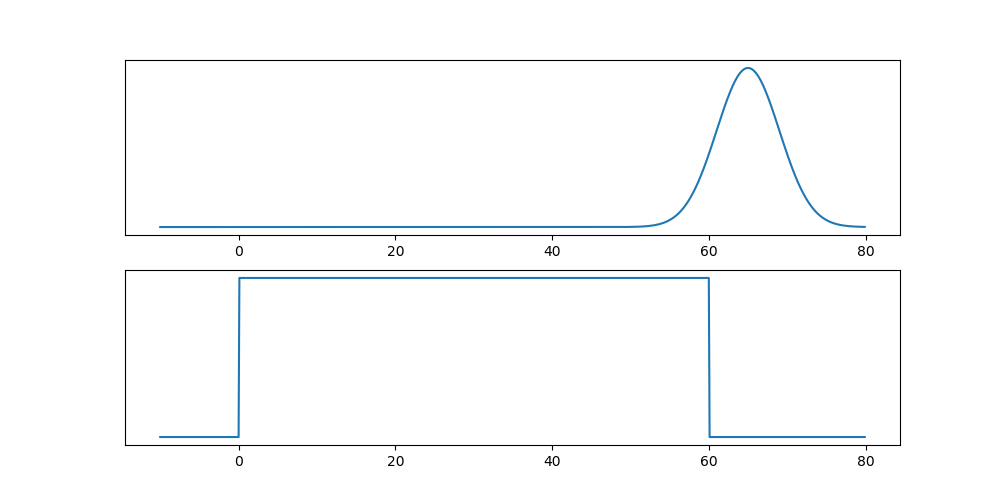
\includegraphics[width=1.0\textwidth]{distributions.png}
\caption{A normal, and uniform, distributions, shown as KDE-like curves.}
\label{distributions}
\end{figure}

If you're interpreting Figure~\ref{distributions} correctly, you can see that
if we generate random numbers from the top distribution, the majority will be
between 60-ish and 70-ish miles per hour, with many near 65 mph and almost
never anything lower than 50 or greater than 80. If we generate them from the
bottom distribution, however, the babies' birth minutes will all be between 0
and 60 but with no particular tendency towards any value in that range more
than any other.

\subsection{Generating normal random numbers}

\index{normal random value}
\index{normal@\texttt{normal()} (NumPy)}

Let's see if that works. The three arguments to \texttt{normal()} are (1) the
mean of the distribution, (2) the standard deviation, and (3) how many random
numbers you actually want. We'll just start with one at a time:

\begin{Verbatim}[fontsize=\small,samepage=true,frame=single,framesep=3mm]
np.random.seed(13)
print(np.random.normal(65,4,1))
\end{Verbatim}
\vspace{-.2in}

\begin{Verbatim}[fontsize=\small,samepage=true,frame=leftline,framesep=5mm,framerule=1mm]
[62.15043735]
\end{Verbatim}

\begin{Verbatim}[fontsize=\small,samepage=true,frame=single,framesep=3mm]
print(np.random.normal(65,4,1))
\end{Verbatim}
\vspace{-.2in}

\begin{Verbatim}[fontsize=\small,samepage=true,frame=leftline,framesep=5mm,framerule=1mm]
[68.01506551]
\end{Verbatim}

\begin{Verbatim}[fontsize=\small,samepage=true,frame=single,framesep=3mm]
print(np.random.normal(65,4,1))
\end{Verbatim}
\vspace{-.2in}

\begin{Verbatim}[fontsize=\small,samepage=true,frame=leftline,framesep=5mm,framerule=1mm]
[64.82198769]
\end{Verbatim}

\begin{Verbatim}[fontsize=\small,samepage=true,frame=single,framesep=3mm]
print(np.random.normal(65,4,1))
\end{Verbatim}
\vspace{-.2in}

\begin{Verbatim}[fontsize=\small,samepage=true,frame=leftline,framesep=5mm,framerule=1mm]
[66.80724935]
\end{Verbatim}

True to form. We keep getting numbers quite close to 65 mph, with a little bit
of variation. Note that if we reset the seed to our original value, our next
call to \texttt{normal()} gives an identical result to the first one, above:

\begin{Verbatim}[fontsize=\small,samepage=true,frame=single,framesep=3mm]
np.random.seed(13)
print(np.random.normal(65,4,1))
\end{Verbatim}
\vspace{-.2in}

\begin{Verbatim}[fontsize=\small,samepage=true,frame=leftline,framesep=5mm,framerule=1mm]
[62.15043735]
\end{Verbatim}

And of course it's easy to generate many speeds at a time (say, eight):

\begin{Verbatim}[fontsize=\small,samepage=true,frame=single,framesep=3mm]
print(np.random.normal(65,4,8))
\end{Verbatim}
\vspace{-.2in}

\begin{Verbatim}[fontsize=\small,samepage=true,frame=leftline,framesep=5mm,framerule=1mm]
[60.81849148 61.8440439  59.95357622 67.25138714 64.02669499 68.65496282
 66.26940369 65.50921312]
\end{Verbatim}

Notice that each time we call \texttt{normal()}, we get an array back (even if
it has only a single value).

By the way, we should sure expect that if we generate many random speeds, and
take their average, it should be pretty darn close to 65 mph:

\begin{Verbatim}[fontsize=\small,samepage=true,frame=single,framesep=3mm]
print(np.random.normal(65,4,1000).mean())                        
\end{Verbatim}

\begin{Verbatim}[fontsize=\small,samepage=true,frame=leftline,framesep=5mm,framerule=1mm]
65.01577962051226
\end{Verbatim}

Yep.

\subsection{Generating uniform random numbers}

\index{uniform random value}
\index{uniform@\texttt{uniform()} (NumPy)}

Uniform random values can be generated the same way, but with the
\texttt{uniform()} function, which takes as its arguments (1) the min, (2) the
max, and (3) the number of desired values:

\begin{Verbatim}[fontsize=\small,samepage=true,frame=single,framesep=3mm]
np.random.seed(13)
print(np.random.uniform(0,60,1))
\end{Verbatim}
\vspace{-.2in}

\begin{Verbatim}[fontsize=\small,samepage=true,frame=leftline,framesep=5mm,framerule=1mm]
[46.66214463]
\end{Verbatim}

This synthetic baby was born at 46.6 minutes past the hour. What about the next
one?


\begin{Verbatim}[fontsize=\small,samepage=true,frame=single,framesep=3mm]
print(np.random.uniform(0,60,1))
\end{Verbatim}
\vspace{-.2in}

\begin{Verbatim}[fontsize=\small,samepage=true,frame=leftline,framesep=5mm,framerule=1mm]
[14.2524732]
\end{Verbatim}

And the next one?

\begin{Verbatim}[fontsize=\small,samepage=true,frame=single,framesep=3mm]
print(np.random.uniform(0,60,1))
\end{Verbatim}
\vspace{-.2in}

\begin{Verbatim}[fontsize=\small,samepage=true,frame=leftline,framesep=5mm,framerule=1mm]
[49.45671196]
\end{Verbatim}

And the next eleven?

\begin{Verbatim}[fontsize=\small,samepage=true,frame=single,framesep=3mm]
print(np.random.uniform(0,60,11))
\end{Verbatim}
\vspace{-.2in}

\begin{Verbatim}[fontsize=\small,samepage=true,frame=leftline,framesep=5mm,framerule=1mm]
[57.94495188 58.35606683 27.20695485 36.54254777 46.53159088 38.49680069
 43.32109377  2.10219145 17.90696825  3.51074951 51.42365656]
\end{Verbatim}

Of course, resetting the seed gives us our original sequence back:

\begin{Verbatim}[fontsize=\small,samepage=true,frame=single,framesep=3mm]
print(np.random.uniform(0,60,5))
\end{Verbatim}
\vspace{-.2in}

\begin{Verbatim}[fontsize=\small,samepage=true,frame=leftline,framesep=5mm,framerule=1mm]
[46.66214463 14.2524732  49.45671196 57.94495188 58.35606683]
\end{Verbatim}

(Check those numbers with the previous ones to convince yourself.)

And finally, let's sanity check the average:

\begin{Verbatim}[fontsize=\small,samepage=true,frame=single,framesep=3mm]
print(np.random.uniform(0,60,1000).mean())                       
\end{Verbatim}
\vspace{-.2in}

\begin{Verbatim}[fontsize=\small,samepage=true,frame=leftline,framesep=5mm,framerule=1mm]
29.2049841447296
\end{Verbatim}

Yay. ``On average,'' our thousand synthetic babies are born at about half past
the hour, which is what we'd expect.


\section{Generating categorical random values}

\index{random value}
\index{categorical random value}
\index{choice@\texttt{choice()} (NumPy)}

NumPy also provides a way to generate \textit{categorical} values with certain
frequencies, through its \texttt{choice()} function. You give it an array of
the possible values, and it chooses one:

\begin{Verbatim}[fontsize=\small,samepage=true,frame=single,framesep=3mm]
np.random.seed(13)
np.random.choice(['Steelers','Redskins','Giants'])
\end{Verbatim}
\vspace{-.2in}

\begin{Verbatim}[fontsize=\small,samepage=true,frame=leftline,framesep=5mm,framerule=1mm]
'Giants'
\end{Verbatim}

\begin{Verbatim}[fontsize=\small,samepage=true,frame=single,framesep=3mm]
np.random.choice(['Steelers','Redskins','Giants'])
\end{Verbatim}
\vspace{-.2in}

\begin{Verbatim}[fontsize=\small,samepage=true,frame=leftline,framesep=5mm,framerule=1mm]
'Steelers'
\end{Verbatim}

(As always, resetting the seed will restart the same sequence of random team
choices from the beginning.)

\pagebreak
\begin{samepage}
Other useful arguments to \texttt{choice()} include:

\begin{compactitem}
\item \texttt{size} -- the number of elements you want in the resulting array.
\item \texttt{replace} -- if \texttt{False}, the elements will be drawn from
your list \textit{without replacement} (meaning once a value is chosen, it
will not be chosen again). This is often useful.
\item \texttt{p} -- a list of \textit{probabilities} (in the range 0 to 1)
specifying how likely each element in the list is to be chosen. (Note these
must sum to 1; and NumPy, stupidly, will not normalize it for you.)
\end{compactitem}
\end{samepage}

To illustrate:

\begin{Verbatim}[fontsize=\footnotesize,samepage=true,frame=single,framesep=3mm]
print(np.random.choice(['Steelers','Redskins','Giants'], size=14, p=[.3,.6,.1]))
\end{Verbatim}
\vspace{-.2in}

\begin{Verbatim}[fontsize=\footnotesize,samepage=true,frame=leftline,framesep=5mm,framerule=1mm]
['Steelers' 'Redskins' 'Redskins' 'Redskins' 'Giants' 'Steelers' 'Steelers'
 'Redskins' 'Redskins' 'Steelers' 'Redskins' 'Giants' 'Steelers' 'Redskins']
\end{Verbatim}

We asked for 14 random teams, and we told it to give us \texttt{Steelers} 30\%
of the time, \texttt{Redskins} 60\%, and \texttt{Giants} only 10\%. I think
you'll agree that the resulting array was pretty faithful to that. (Of course,
you'll get a different random array each time.)

Finally, let's test a large random array and verify that the requested
percentages are approximately correct:

\begin{Verbatim}[fontsize=\small,samepage=true,frame=single,framesep=3mm]
pd.Series(np.random.choice(['Steelers','Redskins','Giants'], size=1000,
    p=[.3,.6,.1])).value_counts() 
\end{Verbatim}
\vspace{-.2in}

\begin{Verbatim}[fontsize=\small,samepage=true,frame=leftline,framesep=5mm,framerule=1mm]
Redskins    584
Steelers    319
Giants       97
dtype: int64
\end{Verbatim}

\index{value\_counts@\texttt{.value\_counts()} (Pandas)}

Our friend the \texttt{.value\_counts()} method confirms that it pretty much
checks out.


      

\chapter{Synthetic data sets}

\index{synthetic data set}

Last chapter we learned the basic skills for generating arrays of random values
-- both numeric and categorical. Now let's apply these to creating
\textbf{synthetic data set}s that contain more than one variable.

We'll concentrate here on the two-variable case, but the idea is easily
extended to three or more. The important new question, now that we know how to
generate single arrays in isolation, is: to what degree do we want our pair
of synthetic variables to be correlated, and how do we make them so?

\section{\textit{Numeric} variables}

\index{association}
\index{Pearson correlation coefficient}
\index{correlation coefficient}
\index{p-value@$p$-value}

Let's start with the case of two numeric variables. As you know from DATA 101,
there can be an association, or not, between them. The Pearson's correlation
coefficient measures this: if its $p$-value is less than our $\alpha$ setting
(typically .05), then we deem there to be a meaningful association, and the $r$
value tells us whether the correlation is positive or negative.

\subsection{Uncorrelated numeric variables}

On one extreme, let's say you wanted to create a data set with two completely
\textit{uncorrelated} numeric variables -- like the heights (in inches) and the
SAT scores of a group of college applicants. Then you'd just generate two
arrays, one at a time:

\index{sat\_scores@\texttt{sat\_scores}}
\index{heights@\texttt{heights}}

\begin{Verbatim}[fontsize=\small,samepage=true,frame=single]
heights = np.random.normal(65, 8, 100)
sat_scores = np.random.normal(1000, 300, 100)
\end{Verbatim}

\index{Pearson correlation coefficient}
\index{correlation coefficient}
\index{pearsonr@\texttt{pearsonr()} (SciPy)}

How did I choose those particular means and standard deviations? I made them
up. And I played with them until they looked reasonable.

Scatter plotting these (see left side of Figure~\ref{uncorrscatter},
p.~\pageref{uncorrscatter}), and running a Pearson correlation, should reveal
they are independent of each other:

\begin{Verbatim}[fontsize=\small,samepage=true,frame=single,framesep=3mm]
plt.scatter(heights, sat_scores)
plt.xlabel("height (in)")
plt.ylabel("SAT score")
print(scipy.stats.pearsonr(heights,sat_scores))
\end{Verbatim}
\vspace{-.2in}

\begin{Verbatim}[fontsize=\small,samepage=true,frame=leftline,framesep=5mm,framerule=1mm]
(-0.025053425275878834, 0.8045806864145338)
\end{Verbatim}

A $p$-value of .8046 says ``nope, not significantly correlated.'' And of course
there's no reason why they should be: we just generated two different random
arrays, for different ranges.

Incidentally, you might be troubled by the fact that a few of our SAT scores
are outside the legal range:

\begin{Verbatim}[fontsize=\small,samepage=true,frame=single,framesep=3mm]
print("min: {}, max: {}".format(sat_scores.min(), sat_scores.max()))
\end{Verbatim}
\vspace{-.2in}

\begin{Verbatim}[fontsize=\small,samepage=true,frame=leftline,framesep=5mm,framerule=1mm]
min: 304.29, max: 1618.35
\end{Verbatim}

\index{clip@\texttt{.clip()} method (NumPy)}

Real SAT scores are supposed to range between 400 and 1600, the Internet tells
me. We could fix this by using the NumPy \texttt{.clip()} method, which imposes
a high and low cutoff as its arguments:

\begin{Verbatim}[fontsize=\small,samepage=true,frame=single,framesep=3mm]
sat_scores = sat_scores.clip(400,1600)
print("min: {}, max: {}".format(sat_scores.min(), sat_scores.max()))
\end{Verbatim}
\vspace{-.2in}

\begin{Verbatim}[fontsize=\small,samepage=true,frame=leftline,framesep=5mm,framerule=1mm]
min: 400.0 max: 1600.0
\end{Verbatim}

The revised scatter plot is shown on the right side of Figure~\ref{uncorrscatter}.

\begin{figure}[ht]
\centering
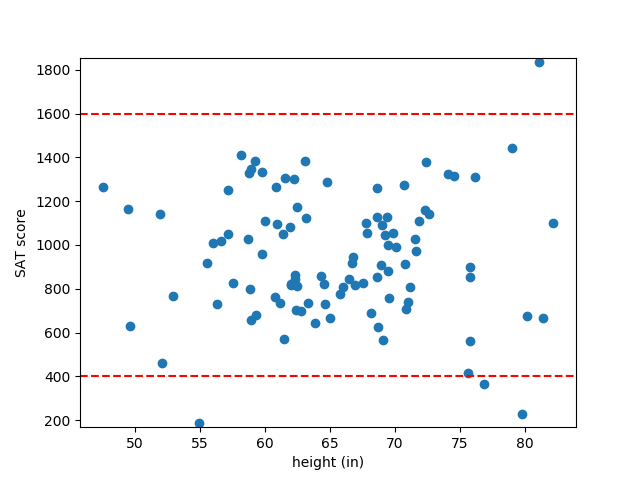
\includegraphics[width=0.45\textwidth]{uncorrscatter.png}
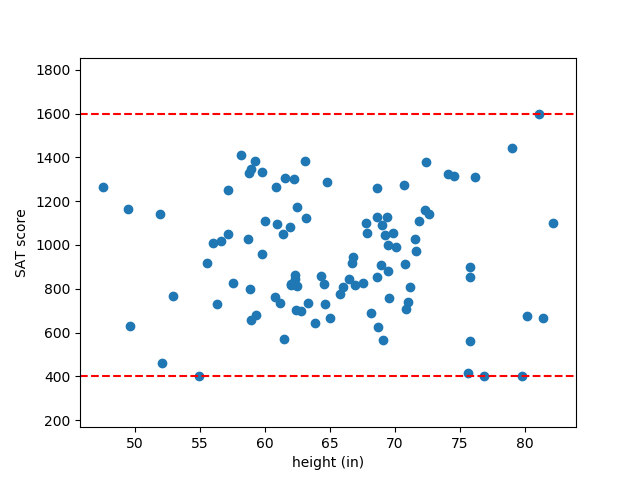
\includegraphics[width=0.45\textwidth]{uncorrscatterclip.png}
\smallskip
\caption{Uncorrelated numeric random variables. The right-hand plot has SAT
scores ``clipped'' to stay above 400 and below 1600.}
\label{uncorrscatter}
\end{figure}



\subsection{Totally correlated numeric variables}

On the other extreme, if two variables are \textit{completely} correlated, then
one is simply a direct (linear) function of the other. That's easy to
accomplish by creating only \textit{one} randomly, and then using it to compute
the other:

\begin{Verbatim}[fontsize=\small,samepage=true,frame=single]
weights_lbs = np.random.normal(150, 30, 100)
weights_kg = weights_lbs / 2.2
\end{Verbatim}

Clearly a person's weight in pounds completely determines their weight in
kilograms: all you do is divide by a constant factor to convert between units.

\begin{figure}[ht]
\centering
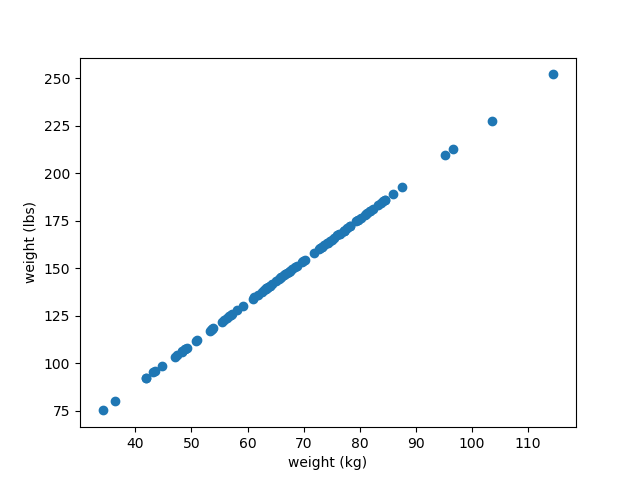
\includegraphics[width=0.45\textwidth]{compcorrscatter.png}
\smallskip
\caption{Two \textit{completely} correlated numeric variables.}
\label{compcorrscatter}
\end{figure}

Scatter plotting these gives a perfectly straight line (see
Figure~\ref{compcorrscatter}), and Pearson tells us they're totally correlated
(the $p$-value is rock bottom 0.0, and $r$=1):

\index{pearsonr@\texttt{pearsonr()} (SciPy)}

\begin{Verbatim}[fontsize=\small,samepage=true,frame=single,framesep=3mm]
print(scipy.stats.pearsonr(weights_lbs,weight_kg))
\end{Verbatim}
\vspace{-.2in}

\begin{Verbatim}[fontsize=\small,samepage=true,frame=leftline,framesep=5mm,framerule=1mm]
(1.0, 0.0)
\end{Verbatim}

\subsection{Somewhat correlated numeric variables}

Now let's take the most common and interesting case: a data set in which our
two numeric variables are \textit{partially}, but not completely, correlated.
(By ``partially correlated'' I just mean that there \textit{is} an association
between the variables, but it's not a rigidly perfect one, like the one between
weight-in-pounds and weight-in-kg.)

\index{noise}

What we'll do is first generate one of the variables independently and
randomly, and then compute the second as a function of the first \textit{with
added \textbf{noise}}. ``Noise'' is a strange (and somewhat misleading) term
that's used in a variety of statistical situations. Here it means ``random
other factors that influence a numeric variable's value up or down.''

\index{SAT}
\index{GPA}

As an example, let's create a synthetic data set with two variables about high
school seniors: her SAT score, and her high school GPA. A moment's thought
will tell you that this indeed falls under our third, ``somewhat correlated''
case: students with better SAT scores also on average tend to have higher GPAs,
but this is an imperfect relationships that doesn't always hold completely.

\index{nudge@``nudge''}

Our strategy is as follows. First, randomly create an array of synthetic SAT
scores. Then, calculate each student's GPA as a function of her SAT score,
plus a random ``nudge'' either up or down to account for other random factors.

\index{white noise}

For our noise factor (the ``nudge'') we'll take the most common approach: a
normally-distributed random variable with a mean of zero. This is called
``\textbf{white noise},'' for various semi-interesting reasons. We use a mean
of 0 for this because on average, we don't want the random ``nudges'' to be
biased in either the up direction or the down direction. On average, we want
the net nudge to be zero.

Okay. Now see if you can understand the two lines of code we use to implement
this strategy:

\index{sat\_scores@\texttt{sat\_scores}}

\begin{Verbatim}[fontsize=\small,samepage=true,frame=single,framesep=3mm]
sat_scores = np.random.normal(1000, 300, 100)
gpas = sat_scores * (2.5 / 1400) + np.random.normal(0, 1, 100)
\end{Verbatim}

The \texttt{sat\_scores} line is the same one we had before. We're then
modeling the high school GPA of a student as \textit{somewhat} correlated with
his SAT score. The ``$\frac{2.5}{1400}$'' multiplier is an attempt to quantify
the relationship between the two variables, which of course are measured on
completely different scales. We're guestimating that a 1400 on the SAT would
kinda sorta equate to about a 2.5 GPA. Notice that the second component of
\texttt{gpas} is a normally distributed noise component \textit{with zero
mean}. (Why a standard deviation of 1? Just a guess. We can tweak it later if
we don't like the results.)

Now this is a good first attempt. Notice two assumptions/limitations, though:

\begin{enumerate}

\item We're assuming that the relationship between the two variables is
\textit{linear} --- namely, that ``the first value times a constant'' is a good
estimate for the second value. In reality, of course, the relationship is often
more complex: it might be better modeled as the \textit{square} of the first
value, for instance, or ``$e$ to the'' first value, or the cube root of the
first value, \textit{etc.}

\index{intercept term}

\item We're assuming that the ``zero point'' for the two variables coincide: in
other words, a zero for one value would on average roughly correspond to a zero
for the other. In the above case, we're assuming that a person who got a 0 on
the SAT would have, on average, a 0 GPA. If this isn't appropriate, we should
add an \textbf{intercept term} (a constant) to our generative formula. This
takes our generated second variable and just shifts it, wholesale, to a new
region of the number range.

\end{enumerate}

We'll stick with the first assumption (linearity) for the moment, but be more
flexible about the second. If we include an intercept term, our formula for
generating the dependent variable boils down to:

\begin{center}

\texttt{dep\_variable} = $m \ \cdot$ \texttt{indep\_variable} + $b$ +
\texttt{np.random.normal(0, $\sigma$, $n$)}

\end{center}

\index{y=mx+b@$y=mx+b$}

which is the familiar equation for a line ($y=mx+b$) with a noise term added
in (with $\sigma$ standard deviation). Now we have to estimate decent values
for $m$, $b$, and $\sigma$. How should we do this?

\medskip

My preferred approach is to identify a ``high-ish'' value of the first
variable, and estimate a (roughly, on average) corresponding value of the
second variable. Then do the same for a ``low-ish'' value. Then, plug those
into the $y=mx+b$ formula and solve for the slope and intercept.

Example: let's generate a synthetic data set of two variables: the number of
hours a person has practiced playing the Dance Dance Revolution (DDR) videogame
in their lifetime, and the score they achieved in a DDR contest (on the song
\textit{Kakumei}). Clearly, there should be some (positive) relationship
between the two quantities: when \texttt{num\_hrs} is high, you'd expect
\texttt{score} to also be high. If you're familiar with the game, though, you
know that the zero points for these variables do \textit{not} coincide: even if
you've never ever played at all, you'll still manage to stumble through the
song, learn how to play as you go, and get a positive score.

Based on my knowledge of the game (which I suck at, by the way), I estimate: 

\begin{compactitem}

\item A decent player who has practiced for 100 hours might get a score of
around 60 million.
%\footnote{For whatever reason, even bad scores in DDR are
%zany high numbers. To avoid writing out tons of zeros, I'll just consider
%``60'' to be a player's score instead of ``60,000,000.''}

\item A sucky-ish player who has practiced for only 10 hours might
get a score of around 30 million.

\end{compactitem}


Running the algebra\footnote{Linear algebra fans can avoid doing all the
mechanical steps by noting that our two equations form the following matrix
equation:
\vspace{-.2in}

\begin{align*}
\begin{bmatrix} 100 & 1 \\ 10 & 1 \end{bmatrix}
\cdot
\begin{bmatrix} m \\ b \end{bmatrix}
=
\begin{bmatrix} 60 \\ 30 \end{bmatrix}
\end{align*}

NumPy can solve this for $m$ and $b$ like so:

\begin{Verbatim}[fontsize=\small,samepage=true,frame=single,framesep=3mm]
X = np.array([[100,1],[10,1]])
Y = np.array([60,30])
print(np.linalg.solve(X,Y))
\end{Verbatim}
\vspace{-.2in}

\begin{Verbatim}[fontsize=\small,samepage=true,frame=leftline,framesep=5mm,framerule=1mm]
[ 0.33333333 26.66666667]
\end{Verbatim}
But only if you're feeling lazy. 
}, I get:
\begin{samepage}
\begin{align*}
60 &= m \cdot 100 + b\\
30 &= m \cdot 10 + b\\
\end{align*}
\vspace{-.7in}
\begin{center}
\dots \textit{insert algebra here} \dots \\
\smallskip
$m = .333, b = 26.667$
\end{center}
\end{samepage}

Thus we get back-of-the-envelope estimates of $m$ and $b$.

Now how to estimate $\sigma$, the standard deviation of the noise term? Play
with it. The larger it is, the more your second variable will deviate from the
perfectly straight line we would predict solely from the $y=mx+b$. Remember
that with the normal distribution, two-thirds of your data points will fall
within one standard deviation from the mean. I think two-thirds of my 100-hour
practicers might get between 50 and 70 million. So I'll go with a
$\sigma$ of 10 and see how that looks.

Finall, here's the actual code to produce a synthetic data set of 200 dancers.
First, generate the practice times themselves:

\index{clip@\texttt{.clip()} method (NumPy)}

\begin{Verbatim}[fontsize=\small,samepage=true,frame=single,framesep=3mm]
num_hrs = np.random.normal(50,20,200).clip(0,500)
\end{Verbatim}

Perhaps your average dancer practiced 50 hours for the competition, with most
of them within 20 hours of that, and no one who practiced less than 0 hours
(not even me), or greater than 500 hours.

Then, we generate these players' scores:

\begin{Verbatim}[fontsize=\small,samepage=true,frame=single,framesep=3mm]
score = num_hrs * .333 + 26.667 + np.random.normal(0,10,200)
\end{Verbatim}

I think it looks pretty decent (Figure~\ref{ddr}).

\begin{figure}[ht]
\centering
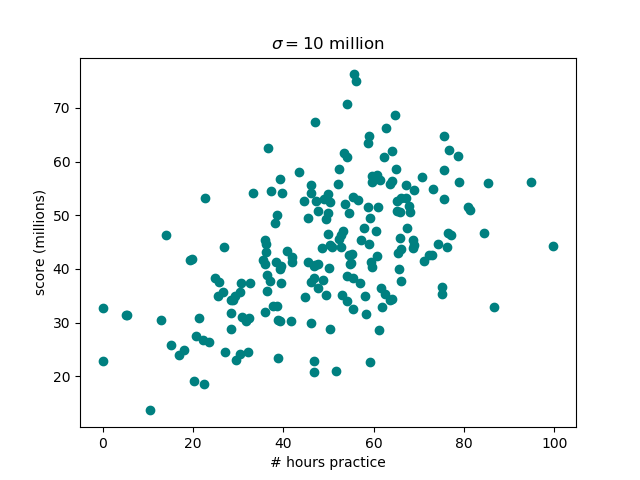
\includegraphics[width=0.46\textwidth]{ddr1.png}
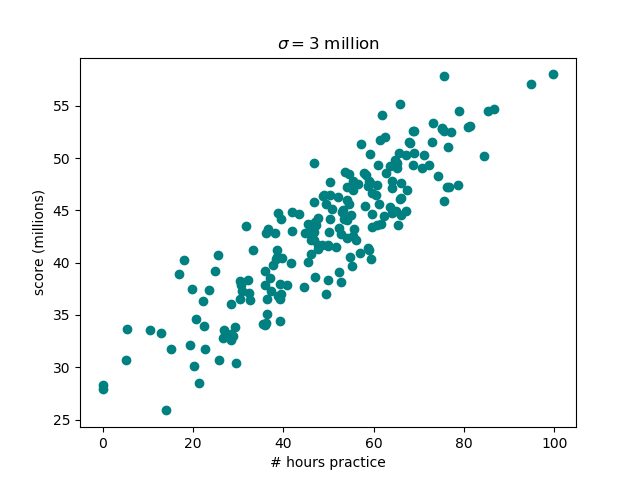
\includegraphics[width=0.46\textwidth]{ddr2.png}
\caption{A scatter plot of two synthetic, partially-but-not-completely
correlated numeric variables. In the left figure, the $\sigma$ for the noise
was set to 10 million; in the right, to 3 million.}
\label{ddr}
\end{figure}

Note: there's also a \texttt{multivariate\_normal()} function in the
\texttt{scipy.stats} package which can generate these kinds of correlated data
sets more powerfully.


%\section{\textit{Categorical} variables}
%
%NumPy provides a way to generate a categorical data set with certain
%frequencies, through its \texttt{np.random.choice()} function:
%
%\begin{Verbatim}[fontsize=\small,samepage=true,frame=single] >>>
%np.random.choice(['Steelers','Redskins','Giants']) 'Redskins' \end{Verbatim}
%
%Useful arguments include:
%
%\begin{compactitem} \item \texttt{size} -- the number of elements you want in
%the resulting array. \item \texttt{replace} -- if \texttt{False}, the elements
%will be drawn from your list \textit{without replacement} (meaning once a
%value is chosen, it will not be chosen again). This is often useful. \item
%\texttt{p} -- a list of \textit{probabilities} (in the range 0 to 1)
%specifying how likely each element in the list is to be chosen. (Note these
%must sum to 1; and NumPy, stupidly, will not normalize it for you.)
%\end{compactitem}
%
%A more complicated example:
%\begin{Verbatim}[fontsize=\footnotesize,samepage=true,frame=single] >>>
%np.random.choice(['Steelers','Redskins','Giants'], size=10, p=[.3,.6,.1])
%['Redskins' 'Redskins' 'Giants' 'Redskins' 'Redskins' 'Steelers' 'Redskins'
%'Steelers' 'Redskins' 'Giants'] \end{Verbatim}
%
%
%\subsection{Uncorrelated categorical variables}
%
%Let's generate a data set with 2000 registered voters in Fredericksburg, 54\%
%Democrats and 46\% Republicans. We'll also generate their pick for the
%Superbowl: Eagles (30\%) or Patriots (70\%).
%
%Since these variables are uncorrelated, we generate each one separately:
%
%\begin{Verbatim}[fontsize=\footnotesize,samepage=true] party =
%np.random.choice(['Democrat','Republican'], p=[.54,.46], size=2000) superbowl
%= np.random.choice(['Eagles','Patriots'], p=[.3,.7], size=2000) \end{Verbatim}
%
%As expected, a $\chi^2$ test's p-value shows no correlation:
%
%\begin{Verbatim}[fontsize=\footnotesize,samepage=true] >>>
%pd.crosstab(superbowl,party) Democrat  Republican Eagles         334 286
%Patriots       746         634
%
%>>> round(scipy.stats.chi2_contingency(pd.crosstab(superbowl,party))[1],2)
%0.98 \end{Verbatim}
%
%\subsection{Completely correlated categorical variables}
%
%Now let's add a ``\texttt{party\_color}'' categorical variable that gives the
%associated color of each voter's political party (blue for Democrats and red
%for Republicans). Since this is perfectly correlated with \texttt{party}, we
%can generate another vector from scratch with the same setup. The
%\texttt{np.where()} function comes in handy:
%
%\begin{Verbatim}[fontsize=\footnotesize,samepage=true] party_color =
%np.where(party=='Democrat','blue','red') \end{Verbatim}
%
%\texttt{np.where()} is tricky but powerful. It takes three arguments -- a
%vector of booleans (\texttt{True}s and \texttt{False}s), and two other
%arguments which are used as substitutions. It produces a vector \textit{that
%includes the second argument in every position where the first is
%\texttt{true}, and the third argument everywhere it's \texttt{false}.} In the
%current example, we're saying ``for every place that the \texttt{party} vector
%has a \texttt{\textquotesingle Democrat\textquotesingle } value, put
%\texttt{\textquotesingle blue\textquotesingle } in this new vector you're
%making for me, and put \texttt{\textquotesingle red\textquotesingle }
%everywhere else.''
%
%We thus (obviously) get perfect correlation:
%
%\begin{Verbatim}[fontsize=\footnotesize,samepage=true] In [30]:
%pd.crosstab(party,party_color) Out[30]: blue  red Democrat    1080    0
%Republican     0  920
%
%>>> round(scipy.stats.chi2_contingency(pd.crosstab(party, party_color))[1],2)
%0.0 \end{Verbatim}
%
%\subsection{Somewhat correlated categorical variables}
%
%Finally, let's create a ``\texttt{gun\_owner}'' categorical variable which has
%the value \texttt{True} or \texttt{False} for each voter: it should be true
%for roughly 44\% of Republicans and for 20\% of Democrats. For this, we can go
%back to our friend \texttt{np.where()}:
%
%\begin{Verbatim}[fontsize=\footnotesize,samepage=true] gun_owner =
%np.where(party=='Democrat',
%np.random.choice([True,False],p=[.2,.8],size=2000),
%np.random.choice([True,False],p=[.44,.56],size=2000)) \end{Verbatim}
%
%This time, our second and third arguments to \texttt{np.where()} are
%\textit{vectors themselves}. We're saying, ``in every position where
%\texttt{party} has a \texttt{\textquotesingle Democrat\textquotesingle }, use
%the corresponding value from our random vector that is 80\% \texttt{false}s.
%Otherwise, use the corresponding value from a different random vector that is
%56\% \texttt{false}s.''
%
%Checking, we do get the desired correlation:
%
%\begin{Verbatim}[fontsize=\footnotesize,samepage=true] >>
%pd.crosstab(party,gun_owner) False  True Democrat      841    239 Republican
%505    415
%
%>> scipy.stats.chi2_contingency(pd.crosstab(party,gun_owner))[1]
%1.5994151557508934e-27 \end{Verbatim}
      

% TODO: in either this chapter or the next, mention keys() as "a relevant thing
% to do" when you're trying to get your head around what a big data set
% contains. (If it's a list (which you can tell with type(s)), you can x[0] it.
% If it's a dictionary, you can keys(x) it and then x['whatever'] it.)

\chapter{JSON (1 of 2)}
\label{ch:JSON1}

JSON (pronounced like the name ``Jason'') is a simple, human-readable text file
format that is very commonly used for information storage and interchange. (It
stands for ``JavaScript Object Notation,'' but don't be fooled: it doesn't have
much to do with the JavaScript language except historically. \textit{Any}
language, including Python, can read/write JSON data.)

In this chapter, we'll learn about how to read and navigate through JSON data.
First, though, a word about a couple of Python essentials I omitted from DATA
101 for brevity and simplicity.

\section{Lists and dictionaries}

\index{series@\texttt{Series} (Pandas)}
\index{ndarray@\texttt{ndarray} (NumPy)}
\index{associative array}
\index{key-value pair}
\index{index}

Last semester, we spent a lot of time learning how to use NumPy
\texttt{ndarray}s and Pandas \texttt{Series}es. These are the preferred
implementations of arrays, and associative arrays, respectively, in the Python
Data Science ecosystem. As you know, a NumPy array holds a numbered sequence of
items (indexed starting from 0), and a \texttt{Series} holds a set of key-value
pairs.

For any serious data work, you want to use those tools, because they are
lightning-fast, super-efficient, feature-rich, and optimized to the task.

\index{plain-ol' Python}

As it turns out, plain-ol' Python has stripped-down, feature-poor, but
easy-to-type versions of these data structures as well, which are baked in to
JSON and also important to know about in their own right. They're called
\textbf{lists} and \textbf{dictionaries}.

\subsection{Lists}

If, instead of writing this:

\begin{Verbatim}[fontsize=\small,samepage=true,frame=single,framesep=3mm]
crew = np.array(["Ed", "Kelly", "Alara", "Bortus", "John", "Claire"])
\end{Verbatim}

you simply wrote this:

\begin{Verbatim}[fontsize=\small,samepage=true,frame=single,framesep=3mm]
crew = ["Ed", "Kelly", "Alara", "Bortus", "John", "Claire"]
\end{Verbatim}

\index{list}

then you get a plain-ol \textbf{list} instead of a NumPy array. It isn't nearly
as fast, nor can it store nearly as many items, and you can't do broadcasting
operations and such with it, but it does the basic job. For example:

\index{len@\texttt{len()} function!for lists}

\begin{Verbatim}[fontsize=\small,samepage=true,frame=single,framesep=3mm]
print("Captain {} initiating roll call for {} officers:".format(
    crew[0], len(crew)))
for member in crew[1:len(crew)]:
    print("{} reporting for duty, sir!".format(member))
print(crew[0])
\end{Verbatim}

\vspace{-.2in}

\begin{Verbatim}[fontsize=\small,samepage=true,frame=leftline,framesep=5mm,framerule=1mm]
Captain Ed initiating roll call for 6 officers:
Kelly reporting for duty, sir!
Alara reporting for duty, sir!
Bortus reporting for duty, sir!
John reporting for duty, sir!
Claire reporting for duty, sir!
\end{Verbatim}

Working with small lists of items is very, very similar to working with NumPy
arrays, so I'm sure you'll pick this right up.

Incidentally, we've actually used lists several times already, without knowing
it. For instance, this very line of code:

\begin{Verbatim}[fontsize=\small,samepage=true,frame=single,framesep=3mm]
good = np.array(["Janet", "Chidi", "Eleanor", "Michael", "Tahani"])
\end{Verbatim}

is actually first creating a \textit{list}, and then passing that list as an
argument to \texttt{np.array()}. And this code:

\begin{Verbatim}[fontsize=\small,samepage=true,frame=single,framesep=3mm]
alter_egos = pd.Series(['Hulk','Spidey','Iron Man','Thor'],
    index=['Bruce','Peter','Tony','Thor'])
\end{Verbatim}

creates two separate lists, one for the data and one for the index, and passes
those to \texttt{pd.Series()} to build a \texttt{Series} out of them. Lists are
super-lightweight and super-common.

\subsection{Dictionaries}

\index{series@\texttt{Series} (Pandas)}
\index{dictionary}
\index{key-value pair}

As mentioned in section~\ref{mentionDictionary}
(p.~\pageref{mentionDictionary}), \textbf{dictionaries} are like stripped-down
Pandas \texttt{Series}es, in the same way that lists are like stripped-down
NumPy arrays. Dictionaries contain key-value pairs, accessed in the same sort
of way (with the boxie \texttt{[]} syntax). You create a dictionary by
using the syntax from p.~\pageref{mentionDictionary2}:

\begin{Verbatim}[fontsize=\small,samepage=true,frame=single,framesep=3mm]
alter_egos = { 'Bruce':'Batman', 'Dick':'Robin', 'Diana':'Wonder Woman',
    'Clark':'Superman' }
\end{Verbatim}

Then, just like with \texttt{Series}es, you can retrieve the value for a key,
change the value for a key, add a new key-value pair, and so forth:

\index{len@\texttt{len()} function!for dictionaries}

\begin{Verbatim}[fontsize=\footnotesize,samepage=true,frame=single,framesep=3mm]
caped_crusaders = [ alter_egos['Bruce'], alter_egos['Dick'] ]
alter_egos['Clark'] = 'Man of Steel'
alter_egos['Victor'] = 'Cyborg'

print("There are now {} heroes, {} of which are the caped crusaders.".format(
    len(alter_egos), len(caped_crusaders)))
print("The dynamic duo is: {} and {}!".format(caped_crusaders[0],
    caped_crusaders[1]))
for key, value in alter_egos.items():
    print("Psssst, {} is really {}...".format(key,value))
\end{Verbatim}
\vspace{-.2in}

\begin{Verbatim}[fontsize=\small,samepage=true,frame=leftline,framesep=5mm,framerule=1mm]
There are now 5 heroes, 2 of which are the caped crusaders.
The dynamic duo is: Batman and Robin!
Psssst, Bruce is really Batman...
Psssst, Dick is really Robin...
Psssst, Diana is really Wonder Woman...
Psssst, Clark is really Man of Steel...
Psssst, Victor is really Cyborg...
\end{Verbatim}

\subsection{Nesting...and nesting, and nesting...}

\index{nested!data structures}

All that was easy so far. The only thing left to tell you -- and man, it can
pack a whammy when you first see it -- is that both lists and dictionaries can
be \textbf{nested} indefinitely. This means that one of a list's elements might
well be another list, or a dictionary. And the value for one of a dictionary's
keys might well be a list, or another dictionary.

Sometimes you have to stare hard at the printout of a nested structure to
figure out how to unpack it. Here are some examples:

\begin{Verbatim}[fontsize=\small,samepage=true,frame=single,framesep=3mm]
a = [ 7, 1, [9, 5], 6 ]
\end{Verbatim}

\index{[]@\texttt{[]} (boxies)}
\index{boxies (square brackets)}

The \texttt{a} variable is a list (you can tell because it starts with a boxie)
and one of its elements happens to be another list (ditto). Stare hard at that,
and then stare hard at this output, and make sure you see why it's so:

\begin{Verbatim}[fontsize=\small,samepage=true,frame=single,framesep=3mm]
print("a[1] is {}".format(a[1]))
print("len(a) is {}".format(len(a)))
print("a[3] is {}".format(a[3]))
print("len(a[2]) is {}".format(len(a[2])))
print("a[2][1] is {}".format(a[2][1]))
\end{Verbatim}
\vspace{-.2in}

\begin{Verbatim}[fontsize=\small,samepage=true,frame=single,framesep=3mm]
a[1] is 1
len(a) is 4
a[3] is 6
len(a[2]) is 2
a[2][1] is 5
\end{Verbatim}

The first one was a warmup. But the second output may have surprised you:
aren't there \textit{five} numbers in that list, not four? The answer is
\textit{no}, there are exactly four:

\begin{compactitem}
\item Item \#0 is the number 7.
\item Item \#1 is the number 1.
\item Item \#2 is a list, which has two elements: 9 and 5.
\item Item \#3 is the number 6.
\end{compactitem}

Once you grasp that, you can probably understand the other outputs from that
example as well. Of particular note is the last one: \texttt{a[2][1]} means
``get element \#2 from \texttt{a}, and since it is itself a list, get element
\#1 from \textit{that}.'' And since all lists are numbered starting with 0,
that's effectively the second element of the third element of \texttt{a}, which
is the number 5.

Next one:

\index{apple}
\index{banana (fruit)}
\index{cherry}
\index{bing cherry}
\index{rainier cherry}

\begin{Verbatim}[fontsize=\small,samepage=true,frame=leftline,framesep=5mm,framerule=1mm]
b = { "apple": 54, "banana": [14, 67], "cherry": { "bing": [ 13, 17,
21], "rainier": { "sweet": "yes", "juicy": "yes" } } }
\end{Verbatim}

\index{\{\}@\texttt{\{\}} (curlies)}
\index{curlies (curly braces)}

The \texttt{b} variable is a dictionary (you can tell because it starts with a
curly) and it contains several key-value pairs. How many, you ask?

\begin{Verbatim}[fontsize=\small,samepage=true,frame=single,framesep=3mm]
print(len(b))
\end{Verbatim}
\vspace{-.2in}

\begin{Verbatim}[fontsize=\small,samepage=true,frame=leftline,framesep=5mm,framerule=1mm]
3
\end{Verbatim}

The three key-value pairs are:

\begin{compactitem}
\item \texttt{"apple"}, whose value is the number 54.
\item \texttt{"banana"}, whose value is a list, whose elements are 14 and 67.
\item \texttt{"cherry"}, whose value is another dictionary. \textit{That}
dictionary has two key-value pairs:
    \begin{compactitem}
    \item \texttt{"bing"}, whose value is a list with 13, 17, and 21.
    \item \texttt{"rainier"}, whose value is yet another dictionary, with keys
\texttt{"sweet"} and \texttt{"juicy"}.
    \end{compactitem}
\end{compactitem}

Now test yourself and make sure you can predict the right output from these
lines of code:

\begin{Verbatim}[fontsize=\small,samepage=true,frame=single,framesep=3mm]
print("b['apple'] is {}".format(b['apple']))
print("b['banana'] is {}".format(b['banana']))
print("len(b['banana']) is {}".format(len(b['banana'])))
print("len(b['cherry']) is {}".format(len(b['cherry'])))
print("len(b['cherry']['bing']) is {}".format(len(b['cherry']['bing'])))
print("b['cherry']['bing'][0]) is {}".format(b['cherry']['bing'][0]))
print("b['cherry']['rainier']['sweet']) is {}".format(
    b['cherry']['rainier']['sweet']))
\end{Verbatim}
\vspace{-.2in}

\begin{Verbatim}[fontsize=\small,samepage=true,frame=leftline,framesep=5mm,framerule=1mm]
b['apple'] is 54
b['banana'] is [14, 67]
len(b['banana']) is 2
len(b['cherry']) is 2
len(b['cherry']['bing']) is 3
b['cherry']['bing'][0]) is 13
b['cherry']['rainier']['sweet']) is yes
\end{Verbatim}

\index{len@\texttt{len()} function!for lists}

Remember, \texttt{len()} plays several roles. When called on a list or array,
it gives the number of elements; on a dictionary or \texttt{Series}, the number
of key-value pairs; on a string, the number of characters; and on a
\texttt{DataFrame}, the number of rows. That's why \texttt{len(b['banana'])}
and \texttt{len(b['cherry'])} both return 2, even though they're very different
types of things.

\index{type@\texttt{type()}}

Note this general rule, too: every time the thing you have is a \textit{list},
you must follow it with an \textit{integer} in boxies. Every time the thing you
have is a \textit{dictionary}, you must follow it with a \textit{key} (often a
string) in boxies. Always.

And now's a good time to mention how to find out what type of thing something
\textit{is} -- the \texttt{type()} function:

\begin{Verbatim}[fontsize=\small,samepage=true,frame=single,framesep=3mm]
print("b['apple'] is a {}".format(type(b['apple'])))
print("b['banana'] is a {}".format(type(b['banana'])))
print("b['cherry'] is a {}".format(type(b['cherry'])))
print("b['cherry']['rainier']['juicy'] is a {}".format(
    type(b['cherry']['rainier']['juicy'])))
\end{Verbatim}
\vspace{-.2in}

\begin{Verbatim}[fontsize=\small,samepage=true,frame=leftline,framesep=5mm,framerule=1mm]
b['apple'] is a int
b['banana'] is a list
b['cherry'] is a dict
b['cherry']['rainier']['juicy'] is a str
\end{Verbatim}

This is super useful when plunging deep through nested data sets.

One last example:

\begin{Verbatim}[fontsize=\small,samepage=true,frame=single,framesep=3mm]
c = [ { 'x': 5 }, [ 14, 'bob', [ 11, { 'duck': 'donuts', 'five':
'guys' }, [ 17, 6 ] ] ] ]
\end{Verbatim}

\index{[]@\texttt{[]} (boxies)}
\index{boxies (square brackets)}

Can you visually line up all those boxies? If so, then you can probably get
these answers correct:

\begin{Verbatim}[fontsize=\small,samepage=true,frame=single,framesep=3mm]
print("len(c) is {}".format(len(c)))
print("c[0]['x'] is {}".format(c[0]['x']))
print("c[1][1] is {}".format(c[1][1]))
print("c[1][2][1]['five'] is {}".format(c[1][2][1]['five']))
print("c[1][2][2][1] is {}".format(c[1][2][2][1]))
print(\end{Verbatim}
\vspace{-.2in}

\begin{Verbatim}[fontsize=\small,samepage=true,frame=leftline,framesep=5mm,framerule=1mm]
len(c) is 2
c[0]['x'] is 5
c[1][1] is bob
c[1][2][1]['five'] is guys
c[1][2][2][1] is 6
\end{Verbatim}



\section{JSON}

\index{JSON}
\index{XML}

Okay, now about JSON proper.

The really nice things about JSON are (1) it's a simple format, and relatively
easy on the eyes (unlike binary formats, or XML), and (2) it structures
information in nested list-ish, dictionary-ish, string-ish type
elements that are exactly like what we covered in the previous section. A JSON
``document'' is, in fact, \textit{essentially a Python list or dictionary with
embedded contents.}

Here's an example file in JSON format:

\begin{Verbatim}[fontsize=\footnotesize,samepage=true,frame=lines,framesep=3mm]
{"name": "Luke Skywalker", "rank": "Jedi", "lightsaber color": "blue",
"episodes": ["IV", "V", "VI", "VIII", "IX"], "relations": {"Leia": "sister",
"Han": "friend", "Artoo": "servant", "Threepio": "servant", "Rey": "student"}}
\end{Verbatim}

Its structure is instantly apparent: a dictionary whose values are strings,
lists, and other dictionaries, as appropriate.

Probably the best thing about JSON is that once we read and parse a JSON file
or other information source, we have a bona fide Python variable that we can
treat in the ordinary way.

In Python, we have the \texttt{json} package, which you can import like any
other:

\begin{Verbatim}[fontsize=\small,samepage=true,frame=single,framesep=3mm]
import json
\end{Verbatim}

There are four functions that matter:
\begin{compactitem}

\item \texttt{json.dump}(\textit{someVariable}, \textit{aFile}) - Dump the
Python variable to a file in JSON text format.

\item \texttt{json.dumps}(\textit{someVariable}) - Dump the Python
variable to a string in JSON text format (and return it).

\item \texttt{json.load}(\textit{aFile}) - Build and return a Python
variable from the contents of the JSON text file.

\label{json.loads}
\item \texttt{json.loads}(\textit{someString}) - Build and return a Python
variable from the JSON text string.

\end{compactitem}

\index{json file@\texttt{.json} file}

So, for instance, to load a file \texttt{info.json} into a Python variable
called ``\texttt{my\_stuff}'':

\begin{Verbatim}[fontsize=\small,samepage=true,frame=single,framesep=3mm]
with open('info.json','r') as f:
    my_stuff = json.load(f)
\end{Verbatim}

We could parse and access the Luke Skywalker file just like this:

\begin{Verbatim}[fontsize=\small,samepage=true,frame=single,framesep=3mm]
with open('luke.json','r') as f:
    luke = json.load(f)
print(luke['lightsaber color'])
blue

print(luke['episodes'][2])
VI
\end{Verbatim}

\normalsize
Simple as that!

\subsection{``Pretty printing''}

\index{pretty printing@``pretty printing''}
\index{wall of text}

One thing I think you'll find useful is the ability to ``\textbf{pretty
print}'' a nested Python structure, like one you read from a JSON file. Instead
of a monolithic wall of text, like many \texttt{.json} files look out of the
box, a pretty printer attempts to format, indent, and put linebreaks in, so
that you can more readily perceive its structure and figure out how to pick out
the parts you want.

A good package for this is the \texttt{pprint} package. First, you have to do
the import:

\index{import@\texttt{import}}

\begin{Verbatim}[fontsize=\small,samepage=true,frame=single,framesep=3mm]
from pprint import pprint
\end{Verbatim}

\index{print()@\texttt{print()} function}
\index{pprint()@\texttt{pprint()} function}

From then on, instead of \texttt{print()}ing a variable, you can
\texttt{pprint()} it. I think you'll agree, the latter is easier to make sense
of:

\begin{Verbatim}[fontsize=\small,samepage=true,frame=single,framesep=3mm]
print(luke)
\end{Verbatim}
\vspace{-.2in}

\begin{Verbatim}[fontsize=\footnotesize,samepage=true,frame=leftline,framesep=5mm,framerule=1mm]
{"name": "Luke Skywalker", "rank": "Jedi", "lightsaber color": "blue",
"episodes": ["IV", "V", "VI", "VIII", "IX"], "relations": {"Leia": "sister",
"Han": "friend", "Artoo": "servant", "Threepio": "servant", "Rey": "student"}}
\end{Verbatim}

\begin{Verbatim}[fontsize=\small,samepage=true,frame=single,framesep=3mm]
pprint(luke)
\end{Verbatim}
\vspace{-.2in}

\begin{Verbatim}[fontsize=\small,samepage=true,frame=leftline,framesep=5mm,framerule=1mm]
{'episodes': ['IV', 'V', 'VI', 'VIII', 'IX'],
 'lightsaber color': 'blue',
 'name': 'Luke Skywalker',
 'rank': 'Jedi',
 'relations': {'Artoo': 'servant',
               'Han': 'friend',
               'Leia': 'sister',
               'Rey': 'student',
               'Threepio': 'student'}}
\end{Verbatim}

As a bonus, it even puts dictionary keys in alphabetical order, so you can find
them more easily.


\section{``Hierarchical'' vs. ``flat'' data}

\index{flat data}
\index{hierarchical data}

So you see that the JSON file format is essentially a textual representation of
an Python variable with arbitrarily nested inner structure. This variable can
be a list or a dictionary, and have embedded lists and dictionaries to any
level of nesting. Here's another example:

\index{courses (JSON file)}
\label{coursesJson}

\begin{Verbatim}[fontsize=\small,samepage=true,frame=lines,framesep=3mm]
[{"prefix": "DATA", "num": 219, "creds": 3, "instructor": "Davies",
"meetings": [{"time": {"day": "TR", "time": "12:30pm"}, "location": {"bldg":
"Trinkle", "room": "B6"}}], "roster": [{"first": "Lady", "last": "Gaga",
"email": "lgaga@umw.edu"}, {"first": "The", "last": "Rock", "email":
"trock@umw.edu"}, ...
\end{Verbatim}

When you disentangle this, you'll realize that what you have is:

\vspace{.1in}

A list, each element of which is:
\vspace{-.1in}
\begin{compactitem}
\item a dictionary, with key/value pairs:
        \begin{compactitem}
        \item \texttt{prefix}: a string
        \item \texttt{num}: an int
        \item \texttt{creds}: an int
        \item \texttt{instructor}: a string
        \item \texttt{meetings}: a list, each element of which is:
            \begin{compactitem}
            \item a dictionary, with key/value pairs:
                \begin{compactitem}
                \item \texttt{time}: a dictionary, with key/value pairs:

\quad\quad \texttt{day}: a string

\quad\quad \texttt{time}: a string

                \item \texttt{location}: a dictionary, with key/value pairs:

\quad\quad \texttt{bldg}: a string

\quad\quad \texttt{room}: a string

                \end{compactitem}
            \end{compactitem}
        \item \texttt{roster}: a list, each element of which is:
            \begin{compactitem}
            \item a dictionary, with key/value pairs:
                \begin{compactitem}
                \item \texttt{first}: a string
                \item \texttt{last}: a string
                \item \texttt{email}: a string
                \end{compactitem}
            \end{compactitem}
        \item ...and possibly other stuff...
        \end{compactitem}
\end{compactitem}

\normalsize

\pagebreak

This kind of structure is called \textbf{hierarchical} data. This is in
contrast to so-called \textbf{flat} data, like a CSV:
\index{CSV file}

\begin{Verbatim}[fontsize=\normalsize,samepage=true,frame=lines,framesep=3mm]
Prefix,Num,Instructor,Creds,Bldg,Room,Day,Time
DATA,219,Davies,3,Trinkle,B6,TR,12:30pm
ENGL,286,Rigsby,3,Combs,112,MWF,11am
CPSC,305,Finlayson,4,Trinkle,B52,MWF,8am
\end{Verbatim}

It should be clear that hierarchical data is intrinsically \textit{more
expressive} than flat data. Rather than each data record being a strict,
identical-length sequence of values, the whole nested structure communicates
order and relationships between subcomponents, like an outline.

It's not even always possible, let alone straightforward, to convert from a
hierarchical format to a flat format. Consider the JSON file on
p.~\pageref{coursesJson}: it permits any number of \texttt{meetings} for a
single course, each of which has embedded structure. In this case, the
structure for each meeting is regular, since it's apparently composed of a
fixed number of fields with unique names. (This won't always be the case, and
if it's not, we would \textit{lose information} in collapsing it to a flat
format.) Even so, though, it's not clear what to do with the multiple meeting
times/locations for a course. Do we make each \texttt{Bldg/Room/Day/Time} group
into its own set of headings in the flat format? This brings with it its own
problems, such as:

\begin{compactenum}
\item How do we associate each group of buildings/rooms/days/times together,
since they're now all individual top-level fields? (Naming conventions seem
like the only solution, and it's awkward.)
\item How do we know the maximum number of such meetings, so as to specify the
width of the table?
\item What do we do for rows which don't have the maximum number of meetings?
Leave the others blank?
\item How do we perform standard queries like ``find all courses that have at
least one meeting in Trinkle?'' (We have to split this up into an awkward query
that separately queries each of the columns and unions the answer.)
\end{compactenum}

There are better ways to organize such data, such as the \textbf{relational
model} that has been ubiquitous in database schema design since Ted Codd
invented it in the 1960's. It allows us to ``normalize'' such data sets and
represent them in multiple, interrelated tables. We'll take a look at this
when we look at SQLite later in the course. Some irregular structures defy
even the relational model, however, which is why some newer database paradigms
(like NoSQL databases) have been developed to get around its limitations.

One important fact to grasp, however, is that at the present state of
technology, \textit{almost all machine learning algorithms are based on a
\textbf{flat} data structure}. There are some quite advanced, cutting-edge
exceptions to this, but really the field of mining hierarchical (and other
non-flat) data formats is still in its infancy. Lots of opportunity to make a
name for yourself here!
           

\chapter{JSON (2 of 2)}
\label{ch:JSON2}

% TODO: A big-ol' memory diagram of the entire "courses" nested structure.

In this chapter we'll cover some common techniques for dealing with JSON data.
Most often, what you end up doing is writing Python code that combs
systematically through the data, surgically extracting the parts you need for
analysis. These parts can then be assembled in NumPy arrays, Pandas
\texttt{DataFrame}s, or whatever, and probed as you're accustomed to.

\index{pretty printing@``pretty printing''}

\label{coursesJsonPretty}

Let's go back to the college courses example from p.\pageref{coursesJson},
pretty printed here:

\index{courses (JSON file)}
\index{json file@\texttt{.json} file}
\index{DATA 219}
\index{Lady Gaga}
\index{Rock, The}

\begin{Verbatim}[fontsize=\small,samepage=true,frame=lines,framesep=3mm]
[{'creds': 3,
  'instructor': 'Davies',
  'meetings': [{'location': {'bldg': 'Trinkle', 'room': 'B6'},
                'time': {'day': 'TR', 'time': '12:30pm'}}],
  'num': 219,
  'prefix': 'DATA',
  'roster': [{'email': 'lgaga@umw.edu', 'first': 'Lady', 'last': 'Gaga'},
             {'email': 'trock@umw.edu', 'first': 'The', 'last': 'Rock'},
             ...,
             ...]
 },
 ...
]
\end{Verbatim}

\index{[]@\texttt{[]} (boxies)}
\index{boxies (square brackets)}
\index{\{\}@\texttt{\{\}} (curlies)}
\index{curlies (curly braces)}
\index{list}
\index{dictionary}

The first brute fact to grasp is that whatever its internal complexities, this
whole thing is \textit{a list of dictionaries}. Not a list of lists, or a
dictionary of dictionaries, or a dictionary of lists, but: a list of
dictionaries. How do we know this? Because the first character is a boxie
(``\texttt{[}'') and the second one is a curly (``\texttt{\{}'').

\section{Printing a class roster}

As a first example of working with this data set, let's say we wanted to simply
print the full names of all the students in the 17th course in this list.
First, let's load the \texttt{.json} file into Python:

\begin{Verbatim}[fontsize=\small,samepage=true,frame=single,framesep=3mm]
import json

with open("courses.json") as f:
    c = json.load(f)
\end{Verbatim}

\index{loop}

Here we've called the outermost structure ``\texttt{c}'', which stands for
``courses'' but is shortened since we'll type it a lot. (Remember that
\texttt{c} is a list -- a very long and complicated list, but still a list.)

And then we do a deep think. Printing all the names clearly requires a loop.
But what exactly do we want to loop through? The answer, after scrutinizing the
above structure, is: we need to find the value of the \texttt{"roster"} key of
the 17th dictionary in the \texttt{c} list. That in turn will be a list, and it
will contain dictionaries, one for each student. (Pause before continuing, look
at the JSON contents from p.~\pageref{coursesJsonPretty}, and see if you agree
with every word of this paragraph.)

So, the loop we want is something like this:

\begin{Verbatim}[fontsize=\small,samepage=true,frame=single,framesep=3mm]
for student in c[16]['roster']: 
    print("{} {} is in {} {}.".format(student['first'], 
        student['last'], c[16]['prefix'], c[16]['num'])) 
\end{Verbatim}
\vspace{-.2in}

\begin{Verbatim}[fontsize=\small,samepage=true,frame=leftline,framesep=5mm,framerule=1mm]
Lady Gaga is in DATA 219.
The Rock is in DATA 219.
Obi-wan Kenobi is in DATA 219.
Amy Klobuchar is in DATA 219.
...
\end{Verbatim}

Success. (Don't worry if you don't get this loop right the first time; it often
takes some tweaking and refinement before it works.) Notice how this code
operates:

\begin{compactenum}

\item We dig fairly deep into \texttt{c} (which is a list), finding its 17th
element (at index 16 of course), which is a dictionary. Then we get the value
of that dictionary's \texttt{"roster"} key. As you can see above, that key's
value is a list.

\item Every time through the loop, the ``\texttt{student}'' variable is set
equal to the next element of this list. And that element, as you can see above,
is a dictionary. The dictionary has two items of interest: \texttt{"first"} and
\texttt{"last"}. We then print the values of these two keys, plus the course
prefix and number. (Note that the course prefix and number come directly from
the \texttt{c[16]} dictionary itself, whereas the first and last names come
from keys of the elements of the inner \texttt{"roster"} list that we're
iterating through.)

\end{compactenum}

\section{Printing \textit{all} the class rosters}

That printed the roster for one class. What about printing the roster for
\textit{all} the classes?

If you think about it, the structure is much the same -- except that instead of
merely iterating through class \#17's list of dictionaries, we want to do it
for \textit{every} class.

\index{nested!loops}

You'll probably realize that this necessitates \textit{another}. All the stuff
we did for class \#17, we now want to do for all the classes, one after
another. So in essence, we wrap the previous code in a nested, outer loop which
will perform it once for each course. Check out the following:

\begin{Verbatim}[fontsize=\small,samepage=true,frame=single,framesep=3mm]
for course in c:
    roster = course['roster']
    for student in roster:
        print("{} {} is in {} {}.".format(student['first'], 
            student['last'], course['prefix'], course['num'])) 
\end{Verbatim}

Observe the nested structure (a \texttt{for} within a \texttt{for}), and the
use of a temporary helper variable (\texttt{"roster"}) to make the code
clearer. Also notice how the \texttt{print()} statement includes information
from both the \texttt{student} and \texttt{course} variables, as appropriate.

This is just the right thing. However, when we run it, we get an error after a
while:

\begin{Verbatim}[fontsize=\small,samepage=true,frame=leftline,framesep=5mm,framerule=1mm]
Lady Gaga is in DATA 219.
The Rock is in DATA 219.
Obi-wan Kenobi is in DATA 219.
...
Elizabeth Jennings is in PSCI 401.
Stan Beeman is in PSCI 401.
Phillip Jennings is in PSCI 401.
...
Tyrion Lannister is in ENGL 101.
Jon Snow is in ENGL 101.
Daenerys Targaryen is in ENGL 101.
...
Han Solo is in CHEM 211.
Poe Dameron is in CHEM 211.
---------------------------------------------------------------------------
KeyError                              Traceback (most recent call last)
     77     for student in roster:
     78         print("{} {} is in {} {}.".format(student['first'], 
---> 79             student['last'], course['prefix'], course['num'])) 
     80 

KeyError: 'last'
\end{Verbatim}

Whoaaaa, what's \textit{dat}?

\subsection{Encountering erroneous/missing data}

This kind of error will happen all the time when you're working with JSON. The
first step is not to panic. The second step is to calmly observe that
apparently, everything was working fine up to a point...and then it suddenly
broke. The third step is to look at that error message and see if you can make
sense out of it. (Often, you can.) And the fourth step is to introduce some
tactical debugging messages into your code, so that you can narrow down the
source of the error.

I assume you've done those first two steps. On to the third: the error message.
It says, quote:

\begin{Verbatim}[fontsize=\normalsize,samepage=true,frame=leftline,framesep=5mm,framerule=1mm]
KeyError: 'last'
\end{Verbatim}

and it evidently happened on line 79, which was in the middle of the
\texttt{print()} statement. Put 2 and 2 together and you'll realize that when
we attempted to extract the value of the \texttt{"last"} key for one of the
dictionaries, \textit{it wasn't there.} That's what ``\texttt{KeyError}'' turns
out to mean: you asked for a particular key but there wasn't one in the
dictionary.

The fourth step is crucial. It marks the difference between fledgling, flailing
novices and cool, critical-thinking experts. We need to insert (temporarily)
one or more \textit{print()} statements into our loop, so that \textit{right
before the program crashes,} we get some crucial insight into what was about
to go wrong.

This takes some practice and some intuition, but in this case let me simply
observe what it makes sense to do. If we were about to access a non-existent
key from a dictionary, it might illuminate things if we printed out the
dictionary immediately before trying that stunt. That way, we'll see the state
of affairs just before the error.

Here's the key line, inserted into the inner loop:

\begin{Verbatim}[fontsize=\small,samepage=true,frame=single,framesep=3mm]
for course in c:
    roster = course['roster']
    for student in roster:
        print("The dict is: {}".format(student))
        print("{} {} is in {} {}.".format(student['first'], 
            student['last'], course['prefix'], course['num'])) 
\end{Verbatim}

Now look at the revised output, below:

\begin{Verbatim}[fontsize=\footnotesize,samepage=true,frame=leftline,framesep=5mm,framerule=1mm]
The dict is: {'email': 'han.solo@corellia.gov', 'first': 'Han', 'last': 'Solo'}
Han Solo is in CHEM 211.
The dict is: {'email': 'dameron@resistance.org', 'first': 'Poe', 'last': 'Dameron'}
Poe Dameron is in CHEM 211.
The dict is: {'email': 'root@dagobah.net', 'first': 'Yoda'}
---------------------------------------------------------------------------
KeyError                                  Traceback (most recent call last)
     78         print("The dict is: {}".format(student))
     79         print("{} {} is in {} {}.".format(student['first'], 
---> 80             student['last'], course['prefix'], course['num'])) 
     81 

KeyError: 'last'
\end{Verbatim}

\index{Yoda}
\index{CHEM 211}
\index{DATA 219}

Aha! Our problem is \texttt{Yoda}, a student in CHEM 211 who doesn't have a
last name.

It takes practice and experience to get a feel for where to insert meaningful
debugging statements. The key question to ask is: ``what do I wish I had known
right before the error occurred?'' Add lines of code to shed light on that
question.


\subsection{Dealing with erroneous/missing data}

Once you've discovered the absence of something you were looking for, you need
to ask yourself what the implications are of it being missing. Sometimes it's a
bona fide data error that means you need to investigate the source of the
information, discard some data points, or something else. Other times (as in
the Yoda case) it's innocuous -- not everyone has a last name, after all -- but
you still have to \textit{deal} with the problem somehow so your program can
continue.

In the case of a missing key which you can sensibly ignore, you can code around
it as follows:

\begin{Verbatim}[fontsize=\small,samepage=true,frame=single,framesep=3mm]
for course in c:
    roster = course['roster']
    for student in roster:
        if 'last' in student:
            print("{} {} is in {} {}.".format(student['first'], 
                student['last'], course['prefix'], course['num'])) 
        else:
            print("{} is in {} {}.".format(student['first'], 
                course['prefix'], course['num'])) 
\end{Verbatim}

\index{in@\texttt{in}}

The important line is the fourth one: ``\texttt{if \textquotesingle
last\textquotesingle~in student:}''. The ``\texttt{in}'' keyword checks to see
whether a dictionary has a certain key or not. In this case, if there is no
\texttt{"last"} key, we want to simply print the first name and go on, not
crash. The output is now satisfactory:

\begin{Verbatim}[fontsize=\small,samepage=true,frame=leftline,framesep=5mm,framerule=1mm]
...
Han Solo is in CHEM 211.
Poe Dameron is in CHEM 211.
Yoda is in CHEM 211.
Emperor Palpatine is in CHEM 211.
Chewie is in CHEM 211.
Rey is in CHEM 211.
...
\end{Verbatim}

The appropriate way to deal with an error like this varies depending on the
situation. This is why you need to back away from the keyboard, take a walk,
and ask yourself, ``what does it \textit{mean} when this value is absent or
corrupt? Does that imply that I need to throw out that data point? Or that
something deep and sinister is going on? Or is there a way to safely ignore
it?''
           
\chapter{LOWESS}

% TODO: add "weighted average" material somewhere.
% TODO: and example of "average of averages" not being the true average (if
% group sizes are different.)

\index{noise}

A common exploratory technique for bivariate, numerical data involves finding a
smooth curve to approximate a noisy data set. The structure of the data -- and
whether there even is a relationship between the two variables at all -- may be
more easily visible from such a curve than from a raw splattering of points.

\section{Best-fit line: ``parametric''}

\index{best-fit line}
\index{least-squares line}
\index{line, best-fit / least-squares}
\index{polyfit@\texttt{polyfit()} (NumPy)}
\index{sort@\texttt{.sort()} (NumPy)}

In your stats class, you probably learned how to compute the best-fit line
to a set of bivariate numerical data points, where ``best fit'' was taken in a
``least squares'' sense (\textit{i.e.}, the line that minimizes the sum of the
squared deviations of the line from the actual data points). It will not
surprise you that it's easy to do this in Python as well, as
shown in Figure~\ref{fig:bestFitCode} (p.~\pageref{fig:bestFitCode}).


\index{polyfit@\texttt{polyfit()} (NumPy)}
\index{polynomial}

NumPy's ``\texttt{polyfit()}'' function stands for ``polynomial fit.'' You'll
recall from high school algebra that a polynomial is a function that involves
only \textit{powers} of your $x$ variable: squares, cubes, and so forth (no
sines, cosines, logarithms, ``$e$-to-the's'' or anything else). Also permitted
are a plain-old $x$ term (since that's $x^1$, or ``$x$ to the first power'')
and a constant term (since that's $x^0$, or ``$x$ to the zeroth power''). And
any of these things can be multiplied by any coefficient you like. So, one
example polynomial would be:

\begin{align*}
y = 4.3 x^3 - 29.4 x^2 + 6 x - 13.8
\end{align*}
\vspace{-.25in}

\index{degree (of a polynomial)}
\index{coefficients (of a polynomial)}

The \textbf{degree} of a polynomial is the highest exponent it contains; this
example has degree 3.

\bigskip
\begin{figure}[hb]
\begin{Verbatim}[fontsize=\footnotesize,samepage=true,frame=single,framesep=3mm]
# Create x points and some crazy, noisy y function of them.
x = np.random.uniform(0,100,100)
x.sort()
y = 4*x - .2 * x**2 + np.random.normal(0,120,100)

# Get the slope and intercept of the best-fit line.
m, b = np.polyfit(x, y, 1)

# Heck, while we're at it let's find the best-fit quadratic too.
a1, a2, a3 = np.polyfit(x, y, 2)

# Plot the points and the approximations.
plt.scatter(x,y)
plt.plot(x, m*x + b,color="green")
plt.plot(x, a1*x**2 + a2*x + a3,color="purple")
\end{Verbatim}
\caption{Finding and plotting the best-fit (least-squares) line. (Note that we
have to \texttt{.sort()} the $x$ points since we draw line plots based on
them, and you get crazy zig-zags if you don't sort your $x$ values first.)}
\label{fig:bestFitCode}
\end{figure}
\bigskip
 

Now the \texttt{polyfit()} function asks: which polynomial can I pick (of a
given degree) that will get the closest to the data points -- \textit{i.e.},
minimize the squared distances between the polynomial's value and the points?
It takes three arguments: an array of $x$ values, an array of $y$ values, and
the degree. It returns the coefficients for the best-fit polynomial of that
degree. So in the Figure~\ref{fig:bestFitCode} code, this line:

\begin{Verbatim}[fontsize=\small,samepage=true,frame=single,framesep=3mm]
m, b = np.polyfit(x, y, 1)
\end{Verbatim}

says ``please give me the coefficients of the best-fit 1-degree polynomial to
these \texttt{x} and \texttt{y} points.'' Since a 1-degree polynomial is a
straight line, we got two coefficients back, which we named \texttt{m} and
\texttt{b}, as is traditionally done. Plotting the actual line was accomplished
with this code:

\begin{Verbatim}[fontsize=\small,samepage=true,frame=single,framesep=3mm]
plt.plot(x, m*x + b,color="green")
\end{Verbatim}

\index{y=mx+b@$y=mx+b$}

which says ``For each $x$ value in the data set, plot $x$ versus $mx+b$.'' And
that, of course, plots the line with slope \texttt{m} and $y$-intercept
\texttt{b}. Similar code plots the best-fit quadratic function (2-degree
polynomial), or any degree we like.

\index{parametric model}

No matter what degree we use, these approximations are called
\textbf{parametric} models because they're based on (global) parameters: a
slope and an intercept, say, or three coefficients in the case of the
quadratic. In each case, we assume the data fit an overall particular
``functional form'' (like a line, or a quadratic) and say, ``given that we feel
like these data are `really' a line, what parameters that describe a line would
give us the best line?''

Figure~\ref{fig:bestFitPlot} (p.~\pageref{fig:bestFitPlot}) shows the best-fit
line and best-fit quadratic (function with an $x^2$ term) for the points
generated by the code in Figure~\ref{fig:bestFitCode}.

\begin{figure}
\centering
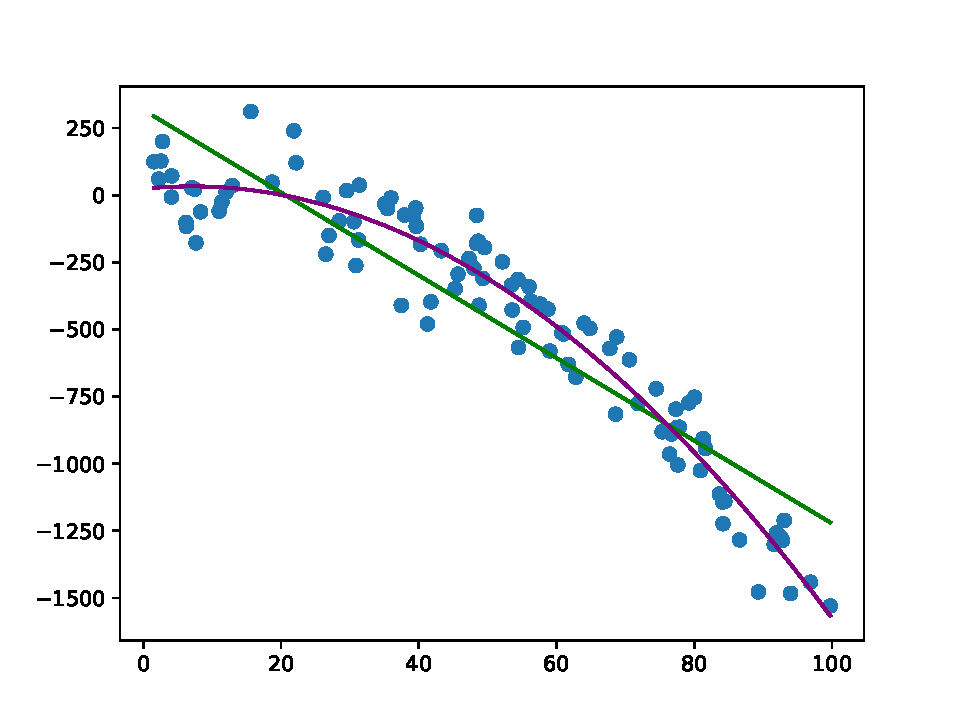
\includegraphics[width=0.8\textwidth,
  alt={Scatter plot of about 100 blue points sloping downward from near 0 at x = 0 to about -1500 at x = 100, curving more steeply toward the right, with two fitted curves: a green straight least-squares line, and a purple least-squares quadratic that bends to follow the points.}]{bestfit.pdf}
\caption{The best-fit line, and best-fit quadratic, to the set of points
generated by the code in Figure~\ref{fig:bestFitCode}.}
\label{fig:bestFitPlot}
\end{figure}
\section{LOWESS: ``non-parametric''}

A more sophisticated technique for this task is called ``\textbf{LOWESS}''
(sometimes ``\textbf{LOESS}''\footnote{Some authors make a very fine
distinction between the LOESS and the LOWESS techniques, which is too nitpicky
to even get into here. We'll treat the two terms as synonymous.}), which
(sorta) stands for ``Locally Weighted Estimated Scatterplot Smoothing.''
LOWESS tries to capture the overall trend of a messy set of data -- but what
distinguishes it from a best-fit line is that it operates \textit{locally}
rather than globally. When you crunch the numbers to find the best-fit
least-squares line to a data set, you're asking, ``what values of slope and
intercept for a \textit{single} line across the \textit{entire} data set will
give me the lowest \textit{overall} deviation from the points?'' (The same is
true for a best-fit quadratic, cubic, \textit{etc.}) In other words, you're
attempting to fit a single model over the entire range of data, and penalizing
inaccuracies equally everywhere.

By contrast, the LOWESS technique approximates the data \textit{locally}. This
means that it weights the data points in such a way that points close to the
location of interest contribute more strongly than do data points farther
away. It does this by fitting a linear (or polynomial) regression to each $x$
point of interest, but using a weighted contribution from only the nearby
points.

Here's how it works. We start with a bunch of $(x,y)$ points, and we want to
compute a ``locally smoothed'' $y$ for every one of the $x$'s. 

First, we have a parameter $\alpha$ that specifies \textit{what fraction of
the data} to take into account (at all) for each estimate. This can be any
value from 0 to 1. You might guess that the smaller it is, the more wiggly
it'll allow our smoothed estimate to be, since we'll be considering only a
small number of points. This is true, as we'll see.

Then, once we've fixed $\alpha$, we're going to find a bunch of best-fit,
least-squares lines, one at each $x$ value. This is just like in regular old
linear regression. The catch is that instead of minimizing the \textit{sum} of
squared differences, we're going to minimize the \textbf{weighted} sum. And
we'll place a greater weight on the errors for $x$ points close to the one
we're evaluating. This will have the effect of allowing the curve to bend
closely to our actual data points while ignoring stuff that's far away.

Written in equations, the ordinary best-fit line approach finds an $m$ and $b$
that minimize the overall sum of squared deviations (or ``residual sum of
squares''):

\begin{align*}
RSS = \sum_i (y_i - (mx_i + b))^2
\end{align*}

But with LOWESS, we calculate this separately for every $x$ point, and we
weight this with a \textbf{weight function} $w$:

\begin{align*}
RSS(x) = \sum_i w(x-x_i) \cdot (y_i - (mx_i + b))^2
\end{align*}

Note how the weight function is given the distance between the $x$ value of
interest and the locations of the actual data points. Since we want to weight
close-by points more heavily, the $w$ should be higher for values closer to
zero.\footnote{\index{kernel} If you're really on your game, you might observe
that the weight function is much like the \textit{kernel} for KDEs: in fact, it
really is basically a kernel. \index{Gaussian (kernel)} Thus we can use a
Gaussian for it, just like we did for KDEs, although it's more common with
LOWESS to use the so-called ``tri-cube'' kernel: $w(\Delta x) = (1 - |\Delta
x|^3)^3$ for $|x|<1$ (and 0 otherwise).}

This is \textbf{non-parametric} because when we're done, if somebody asked,
``hey, I like your LOWESS curve -- what parameters did you use for it?'' the
answer would be ``uh...there really aren't any parameters.'' The curve is a
messy combination of a bunch of different shifting approximations that we
calculated as we went through the whole data set. We didn't choose parameters
to plug into a particular model; in fact, we didn't really \textit{have} a
model.

Like KDEs, this technique wasn't computationally possible until the age of
computers. Hence it's one of the newer kids on the block. Here's how to do it
in Python with the \texttt{statsmodel} library:

\index{import@\texttt{import}}

\begin{Verbatim}[fontsize=\footnotesize,samepage=true,frame=single,framesep=3mm]
from statsmodels.nonparametric.smoothers_lowess import lowess

l = lowess(y,x,frac=1/3)
plt.plot(l[:,0],l[:,1],color="red")
\end{Verbatim}

\index{bias-variance trade-off}
\label{bvTradeoffLowess}

The ``\texttt{frac}'' parameter is our $\alpha$. The resulting curve for two
different values of $\alpha$ is shown in Figure~\ref{fig:lowess}. Notice how
$\alpha = \frac{1}{3}$ gives a much smoother line than $\alpha =
\frac{1}{10}$, since it is using more points to do the smoothing. In fact, the
former is quite close to the best-fit quadratic in this case. This is a
manifestation of the classic ``bias-variance trade-off'' we'll look closely at
in Chapter~\ref{ch:kNN2}.

\begin{figure}[ht]
\centering
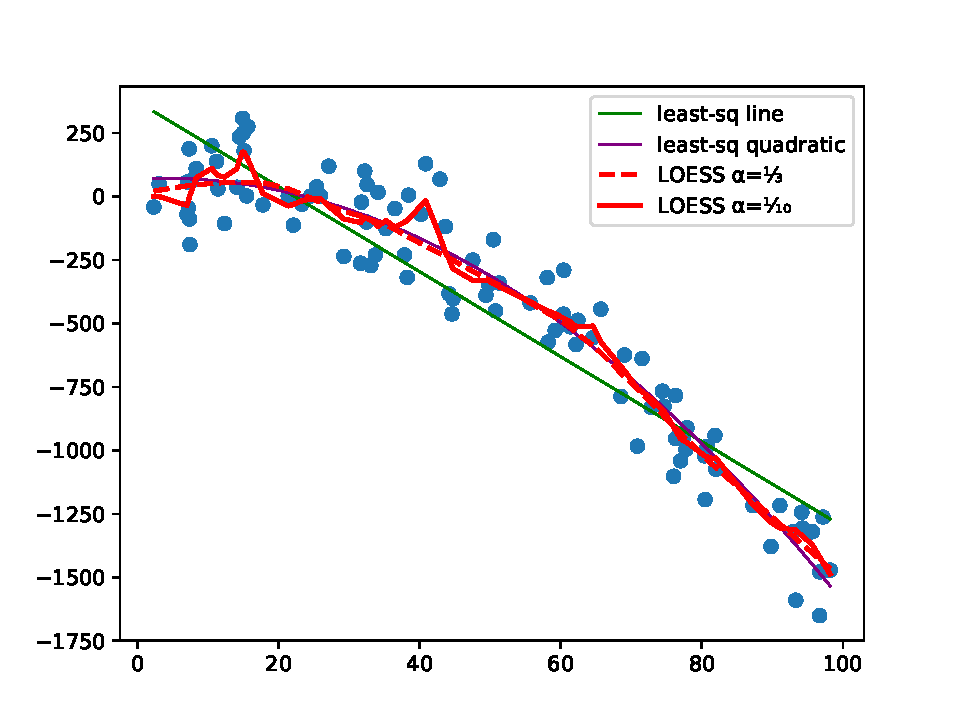
\includegraphics[width=1\textwidth,
  alt={The same noisy downward-curving scatter with four fitted curves per the legend: green least-squares line, purple least-squares quadratic, dashed red LOESS with alpha one third, and solid red LOESS with alpha one tenth. The quadratic and both LOESS curves track the points closely, the alpha one tenth curve with small wiggles.}]{lowess.pdf}
\caption{Various attempts to plot the ``true, underlying pattern'' of our
noisy data set.}
\label{fig:lowess}
\end{figure}

\smallskip

LOWESS might not appear to have much of an advantage over just a plain old
line. But Figure~\ref{fig:lowessBetter} (p.~\pageref{fig:lowessBetter}) shows a
data set where neither the line nor the quadratic are even in the ballpark, yet
where LOWESS does quite well. Intuitively, if the data \textit{aren't}
ultimately generated by something linear (or close to it), a linear model will
be hard-pressed to capture the curve.

\begin{figure}[ht]
\centering
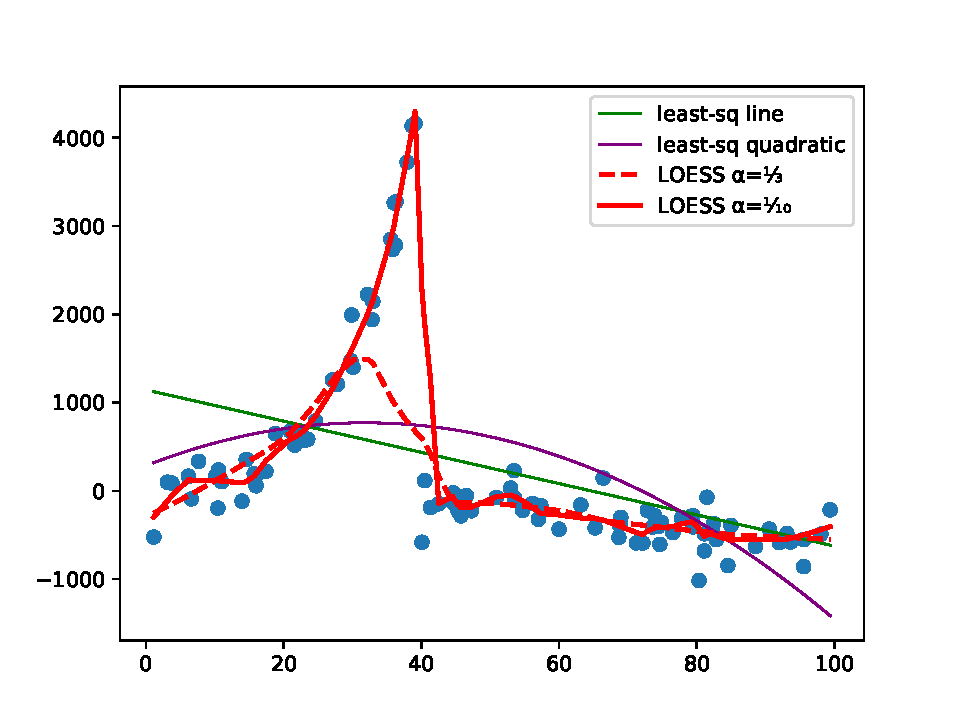
\includegraphics[width=.95\textwidth,
  alt={Scatter plot of about 100 blue points that hover near 0 for x below 20, rise sharply to a spike of about 4000 just before x = 40, then drop back to around -300 and drift slightly downward to x = 100. The green line and purple quadratic miss the spike entirely; the dashed red LOESS with alpha one third rises only to about 1500; the solid red LOESS with alpha one tenth follows the spike almost exactly.}]{lowess_better.pdf}
\caption{A decidedly non-linear data set, for which LOWESS (and particularly
LOWESS with a low $\alpha$) does quite well.}
\label{fig:lowessBetter}
\end{figure}

\medskip
In general, LOWESS is a better \textit{exploratory} technique than best-fit
parametric curves are. This is true for a couple of reasons:

\begin{compactitem}
\itemsep.5em
\item When exploring a data set, you're looking for patterns that stick out,
and you want to let the data speak for itself. You're not coming to the data
with a pre-established model choice and wanting to fit it. LOWESS lets you be
model-agnostic and yet see the forest instead of just trees.

\item LOWESS (and non-parametric methods in general) are ``robust,'' meaning
they aren't as adversely affected by outliers. Consider fitting a least-squares
line to a set of data, and then introducing a couple of outliers near one of
the far ends. This is going to force your global-error-minimizing best-fit line
to swing radically away from the bulk of the data (which it may describe fairly
adequately) in order to try and reach those outliers. Clearly this isn't a good
fit for the data! LOWESS, however, will only ``reach'' for those outliers in
the $x$ range when it gets near those outliers.

% TODO: add plot to demonstrate the above paragraph.

\end{compactitem}

\vspace{.1in}

By the way, although we fit a \textit{linear} function to each local point, we
could fit a quadratic, cubic, or anything else. Here's something to think
about: if we replaced the linear ``$mx+b$'' function with just a constant
``$b$'', then LOWESS becomes simply a weighted moving average. Oooo, deep.

\vspace{.1in}

Finally, remember to play with the $\alpha$ parameter just as you played with
the kernel width and bin size in other exploratory techniques. Remember:
changing this will give you different views on the data, and different views
are good.          
\include{covariance}      

\chapter{Data fusion}

\index{data fusion}

In this chapter we'll introduce the sexy-sounding technique of \textbf{data
fusion}. Data fusion means combining and integrating multiple data sources into
a single data set. This can give you richer, more useful information than any
of the individual data sets could on their own.

\section{Merge operations}

\index{table}
\index{merge}
\index{join!inner}

On the ground, data fusion usually necessitates \textit{merging} multiple
tables together. As we've learned, the \textit{lingua franca} of the data
science world is the rectangular table perfectly reflected by a CSV file: it
has (heterogeneous) rows, it has (homogeneous) columns, and is otherwise flat.
In Pandas we speak of this structure as a \texttt{DataFrame}, of course.

More complicated data sets sometimes consist of \textit{multiple} such tables.
This is especially true if there are different aspects to the data, each of
which is deserving of its own table. The tables are often implicitly related,
as we'll see, through some piece of common information that links them
together logically.

Moreover, there will be times in your career when you want to integrate
multiple \textit{different} data sets in some way, perhaps because each gives
you information on some related aspect of a common phenomenon. Imagine if you
found a data source giving vote totals for various political candidates, and a
different data source documenting the financial donations that their campaigns
received. An obvious question would be: ``to what extent do a candidate's
contributions relate to his/her vote count?'' This kind of analysis is only
possible if the two data sets can be merged in a coherent way, so that the
vote totals for a candidate are properly associated with the contributions to
that same candidate's campaign.

We'll use the term \textbf{merge} (or \textbf{join}) to describe the operation
of connecting two tables/\texttt{DataFrame}s into one, based on a common linking piece
of information. The term \textbf{fusion} is usually restricted to the case
described in the previous paragraph; namely, when the two tables to be joined
are from different data sets entirely.


\section{Merging in Pandas}

The basic idea is that in order to meaningfully merge two \texttt{DataFrames},
one (or more) columns in the first table must be logically linked to one (or
more) columns in the second. ``Logically linked'' usually means ``having the
same values in them.'' 

\index{movies}
\index{roles}
\label{originalDFs}
\begin{figure}[ht]
\centering
\begin{Verbatim}[fontsize=\small,samepage=true,frame=none]
                                  roles:
          actor           film                   salary (millions)
          --------------------------------------------------------
          Downey Jr.      The Avengers           50
          Johansson       The Avengers           20
          DiCaprio        Inception              59
          Hanks           Forrest Gump           70
          Bullock         Gravity                77
          Downey Jr.      Iron Man 3             51
          Hanks           Saving Private Ryan    40
          ...
          
                                  movies:
          title           director               year
          -------------------------------------------
          Inception       Nolan                  2010
          The Avengers    Whedon                 2012
          Forrest Gump    Zemeckis               1994
          Gravity         Cuaron                 2013
          Star Wars       Lucas                  1977
          ...
\end{Verbatim}
\caption{Two \texttt{DataFrame}s from an IMDB-like source.}
\label{fig:imdb}
\end{figure}
 
\index{IMDB}
\index{Johansson, Scarlett}
\index{Downey Jr., Robert}
\index{DiCaprio, Leonardo}
\index{Bullocks, Sandra}
\index{Hanks, Tom}
\index{Nolan, Christopher}
\index{Whedon, Joss}
\index{Inception@\textit{Inception}}
\index{The Avengers@\textit{The Avengers}}
\index{Saving Private Ryan@\textit{Saving Private Ryan}}

For example, consider Figure~\ref{fig:imdb}, which contain two \texttt{DataFrame}s from
a data source like IMDB. There are clearly questions we'd like to ask which
involve both \texttt{DataFrame}s together, rather than each in isolation. For instance,
``have actor salaries been going up over time?'' or ``how often have various
actors worked with specific directors?''

Merging here is simple: we simply identify \textit{the common column} which
unites rows from the two tables. Clearly, it's the film title: we know that
Robert Downey Jr. was directed by Joss Whedon because a Downey-Jr. row in the
\texttt{roles} table has the same film name as a film in a Whedon row in the
\texttt{movies} table.

In database parlance, we call the \texttt{title} column of the \texttt{movies}
table its \textbf{primary key} (PK), and we call the \texttt{film} column of
the \texttt{roles} table a \textbf{foreign key} (FK). The primary key /
foreign key relationship is supposed to suggest that for every row in the
\texttt{roles} table, its \texttt{film} value \textit{will} appear in one row
of the \texttt{movies} table (namely, in that row's \texttt{title} column).

To ``join'' these two \texttt{DataFrame}s all in one fell swoop, we execute a command
like this:

\begin{Verbatim}[fontsize=\small,samepage=true,frame=single,framesep=3mm]
roles_movies = pd.merge(roles,movies,left_on="film",right_on="title")
\end{Verbatim}

This produces a new \texttt{DataFrame} that contains (1) all the columns of the
two, and (2) a row for each pair of original rows that match on their movie
title. Notice we had to specify \textit{two} arguments (besides the table
names) to \texttt{pd.merge()}: ``\texttt{left\_on}'' (for the name of the
merging column in the first \texttt{DataFrame}) and ``\texttt{right\_on}'' (for the
second). If these two columns had the same name, we could just specify a single
argument called ``\texttt{on}'' for the two.

\medskip
The \texttt{roles\_movies} table will look like this:

\bigskip
\label{roles_movies}
\begin{Verbatim}[fontsize=\small,samepage=true,frame=none]
                            roles_movies:
actor      film         salary (millions)  title         director     year
--------------------------------------------------------------------------
Bullock    Gravity      77                 Gravity       Cuaron       2013
DiCaprio   Inception    59                 Inception     Nolan        2010
Johansson  The Avengers 20                 The Avengers  Whedon       2012
Downey Jr. The Avengers 50                 The Avengers  Whedon       2012
....
\end{Verbatim}
\bigskip

(The sequence of the rows is not in general reliable, and you should not depend
on them being in the order you expect.) This \texttt{DataFrame} can be used to
answer either of the questions we posed above, and others.

Note that our new table has some redundant information (the \texttt{film} and
\texttt{title} columns are identical) which you can remove using normal Pandas
operations if you wish.

\section{Odds and ends}

\begin{enumerate}
\itemsep1em
\item Sometimes we want to merge on more than one column; for instance:

\begin{Verbatim}[fontsize=\small,samepage=true,frame=single,framesep=3mm]
df = pd.merge(votes,contribs,left_on=['first_name','last_name'],
        right_on=['candidate_first','candidate_last'])
\end{Verbatim}

This gives us rows in the result only when the values in \textit{both} the
\texttt{first\_name} and \texttt{last\_name} columns of \texttt{votes} match
the \texttt{candidate\_first} and \texttt{candidate\_last} columns of
\texttt{contribs}.

\index{join!inner}

\item The default merge operation we've been doing so far is sometimes called
an ``\textbf{inner join}''. This means that \textit{if there is no
corresponding match for a row in one of the \texttt{DataFrame}s, there will be
no associated row in the result.} This is normally what we want. In the movies
example, if we don't have a row in the \texttt{movies} table for a particular
film, then we don't know the year for that film, and it's (perhaps) pointless
to include any of the actors in that film in the resulting merged \texttt{DataFrame}.

\index{join!outer}
\index{join!left}
\index{join!right}

Sometimes, we want to make sure that every row in the left (or right, or both)
\texttt{DataFrame} appears in the result \textit{at least once}, though, with
corresponding null values if necessary. We can do this by specifying
\texttt{\textquotesingle left\textquotesingle }, \texttt{\textquotesingle right\textquotesingle }, or \texttt{\textquotesingle outer\textquotesingle } as the value of the
\texttt{\textquotesingle how\textquotesingle } argument to \texttt{pd.merge()}:

\begin{Verbatim}[fontsize=\small,samepage=true,frame=single,framesep=3mm]
df = pd.merge(votes,contribs,left_on=['first_name','last_name'],
        right_on=['candidate_first','candidate_last'],how='outer')
\end{Verbatim}

\index{name collision}

\item Sometimes merging two \texttt{DataFrame}s will result in column
\textbf{name collision}s. Suppose, for example, that our \texttt{roles} table
had had a \texttt{year} column indicating the birth year of the actor:

\begin{Verbatim}[fontsize=\small,samepage=true,frame=none]
                            roles:
    actor           year   film                   salary (millions)
    ---------------------------------------------------------------
    Downey Jr.      1965   The Avengers           50
    Johansson       1984   The Avengers           20
    DiCaprio        1974   Inception              59
    Hanks           1956   Forrest Gump           70
    Bullock         1964   Gravity                77
    ...
\end{Verbatim}

Then the resulting \texttt{DataFrame} would need to have two columns named
``\texttt{year}'', with different meanings. Pandas solves this by renaming the
conflicting columns with a ``\texttt{\_x}'' or ``\texttt{\_y}'' suffix,
corresponding to the left/right tables in the join:

\footnotesize
\begin{Verbatim}[fontsize=\footnotesize,samepage=true,frame=none]
                            roles_movies:
actor      year_x   film       salary (millions)   title      director   year_y
-------------------------------------------------------------------------------
Bullock    1964     Gravity    77                  Gravity    Cuaron     2013
DiCaprio   1974     Inception  59                  Inception  Nolan      2010
\end{Verbatim}
\normalsize

(which, of course, you can rename at will via
``\texttt{roles\_movies.columns}''.)

\item Finally, the above examples have all featured ``one-to-many''
relationships between the two tables. (\textit{Many} actors star in
\textit{one} movie.) But sometimes we have a ``many-to-many'' relationship.
Consider the Halloween costumes data set below:

%\begin{samepage}
\begin{Verbatim}[fontsize=\small,samepage=true,frame=single,framesep=3mm]
print(costumes)
\end{Verbatim}
\vspace{-.2in}

\begin{Verbatim}[fontsize=\small,samepage=true,frame=leftline,framesep=5mm,framerule=1mm]
    accessory      costume
0      helmet  Darth Vader
1  lightsaber  Darth Vader
2       crown     Princess
3        wand     Princess
\end{Verbatim}
%\end{samepage}

\begin{samepage}
\begin{Verbatim}[fontsize=\small,samepage=true,frame=single,framesep=3mm]
print(children)
\end{Verbatim}
\vspace{-.2in}

\begin{Verbatim}[fontsize=\small,samepage=true,frame=leftline,framesep=5mm,framerule=1mm]
       child      costume
0     Johnny  Darth Vader
1        Sam  Darth Vader
2  Betty Lou     Princess
3    Wendell      Student
4      Kiara     Princess
\end{Verbatim}
\end{samepage}

In order to represent all these children in their chosen costumes, we need
multiple matches from both \texttt{DataFrame}s for each costume value. This is
because each \texttt{Princess} has more than one accessory, and there are also
multiple children who want to \textit{be} princesses. Therefore, we can
potentially end up with a lot of rows in our result.

\begin{Verbatim}[fontsize=\small,samepage=true,frame=single,framesep=3mm]
print(pd.merge(costumes, children, on="costume"))
\end{Verbatim}
\vspace{-.2in}

\begin{Verbatim}[fontsize=\small,samepage=true,frame=leftline,framesep=5mm,framerule=1mm]
    accessory      costume      child
0      helmet  Darth Vader     Johnny
1      helmet  Darth Vader        Sam
2  lightsaber  Darth Vader     Johnny
3  lightsaber  Darth Vader        Sam
4       crown     Princess  Betty Lou
5       crown     Princess      Kiara
6        wand     Princess  Betty Lou
7        wand     Princess      Kiara
\end{Verbatim}

\index{Wendell}
\index{Darth Vader}
\index{Princess}
\index{Student}
\index{join!outer}
\index{join!right}

Btw, notice that poor \texttt{Wendell} was left out of the merged
\texttt{DataFrame} entirely, since his costume did not have any accessories. We
can include him by doing a ``\textbf{right join}'' (or full ``\textbf{outer
join}'') like this:

\begin{Verbatim}[fontsize=\small,samepage=true,frame=single,framesep=3mm]
pd.merge(costumes, children, on="costume", how="outer")
\end{Verbatim}
\vspace{-.2in}

\begin{Verbatim}[fontsize=\small,samepage=true,frame=leftline,framesep=5mm,framerule=1mm]
    accessory      costume      child
0      helmet  Darth Vader     Johnny
1      helmet  Darth Vader        Sam
2  lightsaber  Darth Vader     Johnny
3  lightsaber  Darth Vader        Sam
4       crown     Princess  Betty Lou
5       crown     Princess      Kiara
6        wand     Princess  Betty Lou
7        wand     Princess      Kiara
8         NaN      Student    Wendell
\end{Verbatim}

\end{enumerate}

The ``\texttt{NaN}'' is the placeholder Pandas uses for rows that didn't match
when doing a left/right/outer join.

\section{``By the way...why?''}

At this point you may be asking, ``if we just have to merge the
\texttt{DataFrame}s to do our analysis, why were they stored that way in the
first place? Why not just have everything in one big CSV file?''

\index{redundancy (of information)}

The answer has to do with \textbf{redundancy of information}. Consider the
merged table on p.~\pageref{roles_movies}). It's not the most compact way of
expressing the information, because certain pieces of data are repeated
unnecessarily.

\index{unnormalized (data set)}

For instance, \textit{The Avengers} was released in 2012. Our data source
needs to record that. But in the merged table, this year would be repeated
\textit{for every actor/actress in the movie.} The same is true for the
director of the film. By performing the merge, we have duplicated lots of
values. In database terms, the data set has become \textbf{unnormalized}. This
isn't always a bad thing, and in terms of performing standard ML (machine
learning) algorithms, it's necessary. But you can see why we wouldn't want the
data permanently stored that way. It consumes extra storage, plus it opens a
Pandora's Box of possible contradictions: what if \texttt{Downey Jr.}'s
\texttt{The Avengers} row said 2012, while \texttt{Johansson}'s said 2014. Who
would we believe?

\index{normalized (data set)}

Database normalization is a larger topic than we have time to fully cover in
this class, but the basics are very simple. Conceptually: \textit{each piece
of information should be stored in one and only one place.} Generally
speaking, when that's true, you have a \textbf{normalized} data set, which is
most appropriate for storage and for communication to other potential users.
Analysts will proceed to unnormalize select parts of it in order to perform
certain analyses.

\section{``Tidy'' data}

The term ``tidy'' to describe a data set has sprung into prominence recently
as a result of the excellent paper by Hadley Wickham (of R fame) who neatly
captured the perils of various data formatting choices.

\begin{compactitem}
\item \textbf{variable} -- a category of something, for which individual
objects have a value. For example: height, gender, center\_field\_distance,
name.
\item \textbf{value} -- an actual individual piece of data corresponding to a
variable for one object. For example: 5'6", female, 390 feet, Kylo Ren.
\item \textbf{observation} -- a particular measurement that comprises all the
information necessary to interpret that measurement. For example: Jeff's
weight was 165 lbs., Jenny's golf score at Field \& Cross Links in the rain
was 88. (In the first example, ``all the information necessary'' includes
``Jeff'' and ``165''; in the second, it includes ``Jenny'', ``Field \& Cross
Links'', ``rainy'', and ``88''.)
\item \textbf{observational unit} -- a collection of all the observations of a
particular type. (``Golf performances'' would be an observational unit,
separate from a ``golfers'' unit which contains information about golfers
themselves, not their particular performances.)
\end{compactitem}

\vspace{.2in}
The rule is: a data set is considered \textbf{tidy} if and only if:
\begin{compactenum}
\item Each observational unit is in its own table. (This is essentially
the same as ``normalized,'' from the previous section.)
\item In each table, each observation forms a row.
\item In each table, each column header is a variable, and the column contains
values.
\end{compactenum}

\vspace{.2in}
This is best visualized by looking at examples of \textit{un}tidy data sets
and rectifying them. Here's one:
\small
\begin{Verbatim}[fontsize=\small,samepage=true,frame=none]
            religion   <$10k   $10-20k  $20-30k  $30-40k   $40-50k  $50-75k
0           Agnostic      27        34       60       81        76      137
1            Atheist      12        27       37       52        35       70
2           Buddhist      27        21       30       34        33       58
3           Catholic     418       617      732      670       638     1116
4  Dont know/refused      15        14       15       11        10       35
...
\end{Verbatim}
\normalsize

The problem here is that \textit{the column headings are actually values, not
variables}. Think about it: ``\texttt{\$10-20k}'' isn't the name of a variable
which might have actual values, but the value (range) itself of some variable.

Two questions: (1) What would the variable be for these column values? Answer:
\textit{Income.} (2) What are the cells themselves representing? Answer:
\textit{Frequency.} (\textit{i.e.}, the number of people polled in the survey
who had that religion and that income level.)

We tidy this with the \texttt{pd.melt()} function:

\begin{Verbatim}[fontsize=\small,samepage=true,frame=single]
tdf = pd.melt(df, ['religion'], var_name='income', value_name='frequency')
\end{Verbatim}

which gives us the tidy version:
\begin{Verbatim}[fontsize=\small,samepage=true,frame=none]
                               religion    income  frequency
           0                   Agnostic     <$10k         27
           1                    Atheist     <$10k         12
           2                   Buddhist     <$10k         27
           3                   Catholic     <$10k        418
          ...
\end{Verbatim}

(Sometimes you'll hear the terms ``\textbf{wide}'' and ``\textbf{long}'' to
refer to the untidy and tidy formats in this sort of example, respectively.)

By the way, the inverse operation of ``melt'' is often called
``\textbf{pivot}''. To reverse the above transformation in Pandas, you should
use:

\begin{Verbatim}[fontsize=\small,samepage=true,frame=single]
df = tdf.pivot(index='religion',columns='income')
\end{Verbatim}

for this operation.


% Exercise:
% load http://cs.umw.edu/~stephen/data219/students.csv and tidy it to:
%
%                      students
%            name  year major    school  creds
%   Mal A. Kenobi  Soph  ECON       UMW     32
%  Jay O. Aniston   Sen  ECON  Richmond     92
%
%               gpas
%             name year   GPA
%   Mal A. Kenobi   So  2.47
%  Jay O. Aniston   Sr  2.30
%      (no NaNs)
%
%           schools
%    school     type   mascot
%       UMW   public   Eagles
%  Richmond  private  Spiders
%
% DELETE the original table.
% now add a column for "urban/rural" to schools table. (We'll call Richmond,
% Fredericksburg, and Charlottesville urban, and the others rural.)
%
% how many students are there?
% how many total year-GPA measurements are there?
% what's the overall GPA?
% how many students in rural vs. urban schools?
% average freshman GPA in rural vs. urban schools?
% visual: do freshmen vs. non-freshmen GPAs differ? (will require another col)
% visual: does avg GPA vary by major? by school? (will require another col)
% scatterplot of creds vs. average-yearly-GPA (ditto)
%
% helpful:
% 1) after splitting out school into separate df:
%  df.drop_duplicates()
% 2) to remove NaN's from GPAs once melted:
%  np.isnan(...)   <-- a ufunc
%  ~   <-- boolean "not" operator
%  (to set up: "gpas = gpas[~np.isnan(gpas.GPA)]")
%  (could also do: "gpas.drop(gpas.index[np.isnan(gpas.GPA)])")
% 3) df.col.str   to perform string operations as ufunc
%  (to set up: "gpa.year = gpa.year.str[3:]")
%
% 


          

\chapter{Long, wide, and ``tidy'' data}

\section{Wide form data}

Consider the following \texttt{DataFrame} (called ``\texttt{g}''), which
contains a professor's grade book for his students:

\begin{Verbatim}[fontsize=\small,samepage=true,frame=single,framesep=3mm]
print(g)
\end{Verbatim}
\vspace{-.2in}

\begin{Verbatim}[fontsize=\small,samepage=true,frame=leftline,framesep=5mm,framerule=1mm]
       name year    Q1    Q2    Q3    Q4    Q5    Q6    Q7    Q8
0   Beyonce   So   9.0  10.0   7.0  10.0   8.0  10.0   9.0  10.0
1     Jay-Z   Jr   7.0  10.0   4.0  10.0  10.0   8.0   3.0  10.0
2    Bortis   Sr   8.0  10.0   7.0   3.0   7.0   7.0   7.0   9.0
3       Han   So   NaN   1.0   NaN  10.0   7.0   8.0   7.0   2.0
4       Mal   Jr   5.0   4.0   9.0   NaN   7.0   2.0   5.0  10.0
5     Inara   Jr   3.0   3.0   4.0  10.0   6.0   4.0   7.0   5.0
6   Obi-wan   So   5.0  10.0   9.0   4.0   1.0   4.0   NaN   2.0
7      Finn   Jr   6.0   3.0   5.0   6.0  10.0   NaN   NaN   3.0
\end{Verbatim}

It's not hard to tell what's going on: each student's name and year in school
is recorded, as is their grade on the eight class quizzes. Some students took
zeroes on one of more quizzes (like \texttt{Han} did for quizzes 1 and 3), and
the quiz grades range from 0 to 10.

\index{wide form}

The structural style for this kind of \texttt{DataFrame} is called \textbf{wide
form}. Each piece of a student's data is in its own column, making the
\texttt{DataFrame} quite ``wide,'' and comparatively not very long (tall).

Now there's nothing wrong with wide form. All the data is there, and it allows
us to ask many questions easily, like:

\begin{compactitem}
\item[\leftthumbsup] What was Inara's score on Quiz \#5? \ (\texttt{g[g.name=="Inara"].Q5})
\item[\leftthumbsup] What was the high score on Quiz \#3? \ (\texttt{g.Q3.max()})
\item[\leftthumbsup] What was Mal's average quiz score? \ 
(\texttt{g[g.name=="Mal"].mean(axis=1)})
\end{compactitem}

\smallskip
Other kinds of questions, though, defy easy answers, like these:

\begin{compactitem}
\item[\leftthumbsdown] What was the overall average score (for all quizzes)? \ (?)
\item[\leftthumbsdown] How did class performance compare between the first half
of the semester (quizzes 1-4) and the second half (quizzes 5-8)? \ (?)
\item[\leftthumbsdown] How did freshmen, sophomores, juniors, and seniors
compare? \ (?)
\end{compactitem}

The reason these questions are difficult are that we have quiz scores spread
across different columns. As long as we're happy treating them in groups like
that, it's easy, but as soon as we want to carve up the quiz scores in some
other way, it becomes hard.

\section{Long form data}

\index{melt@\texttt{melt()} (Pandas)}

The solution is to convert the \texttt{DataFrame} to a structure which
collapses all the quiz data into a single column. For this, we use the
\texttt{melt()} function from the Pandas package:

\begin{Verbatim}[fontsize=\small,samepage=true,frame=single,framesep=3mm]
gl = pd.melt(g, ["name","year"], var_name="quiz", value_name="score")
\end{Verbatim}

Now this is kind of complicated so pay attention. 

\index{list}

\begin{compactitem}

\item The first argument is the name of the wide-form \texttt{DataFrame} you
want to ``melt.''

\item The second argument is a list of the columns \textit{that you want to
leave alone.} In other words, a list of ``off-limits'' columns that you want
Pandas \textit{not} to melt.

\item The third argument, named \texttt{var\_name}, is \textit{the name you
want for your new column whose values will be the old column
\underline{names}.} It can be hard to get your head around this one. You have
to imagine all the current column names that you're melting being put in a
column, and ask yourself: ``what is the right name for that new column?'' In
this case, since we're melting \texttt{Q1}, \texttt{Q2}, \textit{etc.}, the
right name for the column is something like ``\texttt{quiz},'' since those are
the quiz numbers.

\item Finally, the fourth argument, named \texttt{value\_name}, is \textit{the
name you want for your new column whose values will be the old column's
\underline{values}.} You have to ask yourself: ``what are those 'things' that
are currently values in the \texttt{Q1}, \texttt{Q2}, \textit{etc.} columns?''
A reasonable answer would be ``\texttt{score},'' since each one is a quiz
score.

\end{compactitem}

We set the result of the \texttt{melt()} call to a variable called \texttt{gl}
(where ``\texttt{l}'' stands for ``long.'') Here's what it looks like:

\begin{Verbatim}[fontsize=\small,samepage=true,frame=single,framesep=3mm]
print(gl)
\end{Verbatim}
\vspace{-.2in}

\begin{Verbatim}[fontsize=\small,samepage=true,frame=leftline,framesep=5mm,framerule=1mm,xleftmargin=2cm]
       name year quiz  score
0   Beyonce   So   Q1    9.0
1     Jay-Z   Jr   Q1    7.0
2    Bortis   Sr   Q1    8.0
3       Han   So   Q1    NaN
4       Mal   Jr   Q1    5.0
5     Inara   Jr   Q1    3.0
6   Obi-wan   So   Q1    5.0
7      Finn   Jr   Q1    6.0
8   Beyonce   So   Q2   10.0
9     Jay-Z   Jr   Q2   10.0
10   Bortis   Sr   Q2   10.0
11      Han   So   Q2    1.0
12      Mal   Jr   Q2    4.0
13    Inara   Jr   Q2    3.0
14  Obi-wan   So   Q2   10.0
15     Finn   Jr   Q2    3.0
16  Beyonce   So   Q3    7.0
17    Jay-Z   Jr   Q3    4.0
18   Bortis   Sr   Q3    7.0
19      Han   So   Q3    NaN
20      Mal   Jr   Q3    9.0
21    Inara   Jr   Q3    4.0
22  Obi-wan   So   Q3    9.0
23     Finn   Jr   Q3    5.0
            . . .
60      Mal   Jr   Q8   10.0
61    Inara   Jr   Q8    5.0
62  Obi-wan   So   Q8    2.0
63     Finn   Jr   Q8    3.0
\end{Verbatim}

\index{long form}

This is called \textbf{long form}, for obvious reasons. We now have one row for
every single quiz score. It might seem wordy, and I'll admit it's not as
easy to locate and eyeball a single result. However, all our ``hard'' questions
from above can be easily answered:

\begin{compactitem}
\item[\leftthumbsup] What was the overall average score (for all quizzes)? \
(\texttt{gl.score.mean()})
\item[\leftthumbsup] How did class performance compare between the first half
of the semester (quizzes 1-4) and the second half (quizzes 5-8)? \\
(\texttt{gl[gl.quiz.isin(["Q1","Q2","Q3","Q4"])].mean()})
\item[\leftthumbsup] How did freshmen, sophomores, juniors, and seniors
compare? \\ (\texttt{gl.groupby("year").score.mean()})
\end{compactitem}

Turning what were column headings into \textit{values} gave us all the
flexibility we needed. We can still treat all the scores individually by quiz
if we want to, but we can also treat them as a whole, or aggregate them in
other ways (like by school year).

As an aside, one thing I'd probably do to this \texttt{DataFrame} is get rid of
the leading ``\texttt{Q}'' before each \texttt{quiz} value, and convert that
column to integers to boot:

\begin{Verbatim}[fontsize=\footnotesize,samepage=true,frame=single,framesep=3mm,xleftmargin=1cm]
gl.quiz = gl.quiz.str[1]
gl.quiz = gl.quiz.astype(int)
print(gl)
\end{Verbatim}

\vspace{-.2in}

\begin{Verbatim}[fontsize=\scriptsize,samepage=true,frame=leftline,framesep=5mm,framerule=1mm,xleftmargin=1cm]
       name year  quiz  score
0   Beyonce   So     1    9.0
1     Jay-Z   Jr     1    7.0
2    Bortis   Sr     1    8.0
3       Han   So     1    NaN
4       Mal   Jr     1    5.0
5     Inara   Jr     1    3.0
6   Obi-wan   So     1    5.0
7      Finn   Jr     1    6.0
8   Beyonce   So     2   10.0
9     Jay-Z   Jr     2   10.0
10   Bortis   Sr     2   10.0
11      Han   So     2    1.0
12      Mal   Jr     2    4.0
13    Inara   Jr     2    3.0
14  Obi-wan   So     2   10.0
15     Finn   Jr     2    3.0
16  Beyonce   So     3    7.0
17    Jay-Z   Jr     3    4.0
18   Bortis   Sr     3    7.0
\end{Verbatim}

\index{str suffix@\texttt{.str} suffix (Pandas)}

The ``\texttt{.str}'' suffix, you'll recall, lets us perform standard string
operations (like \texttt{len()}, \texttt{contains()}, or indexing) on entire
\texttt{DataFrame} columns. Here, by saying ``\texttt{gl.quiz.str[1]}'', we're
requesting only the \textit{second} character (character \#1) of each string,
which extracts the ``\texttt{1}'' from ``\texttt{Q1}'' and so forth.

Treating quiz numbers like the integers they are is conceptually correct, and
also allows us to do things like query for things like ``quizzes after quiz
\#3'' instead of having to list a bunch of categorical values.

\section{``Tidy'' data}

\index{Wickham, Hadley}

The term ``tidy'' to describe a data set has sprung into prominence recently
as a result of the excellent paper by Hadley Wickham (of R fame) who neatly
captured the perils of various data formatting choices. Hadley first defines
these terms:

\begin{compactitem}
\item \textbf{variable} -- a category of something, for which individual
objects have a value. Examples: name, height, gender, center field distance.
\item \textbf{value} -- an actual individual piece of data corresponding to a
variable for one object. Examples: Kylo Ren, 5'6", female, 390 feet.
\item \textbf{observation} -- a particular measurement that comprises all the
information necessary to interpret that measurement. Examples: Jeff's
weight was 165 lbs., Jenny's golf score at Field \& Cross Links in the rain
was 88. (In the first example, ``all the information necessary'' includes
``Jeff'' and ``165''; in the second, it includes ``Jenny'', ``Field \& Cross
Links'', ``rainy'', and ``88''.)
\item \textbf{observational unit} -- a collection of all the observations of a
particular type. (``Golf performances'' would be an observational unit,
separate from a ``golfers'' unit which contains information about golfers
themselves, not their particular performances.)
\end{compactitem}

\index{tidy@``tidy'' data}

\vspace{.2in}

Then, he outlined one simple rule. A data set is considered \textbf{tidy} if
and only if:

\definecolor{shadecolor}{rgb}{.9,.9,.9}
\begin{shaded}
\begin{compactenum}
\item \label{ownTable} Each observational unit is in its own table.
\item \label{obsRow} In each table, each observation forms a row.
\item \label{colHeader} In each table, each column header is a variable, and
the column contains values.
\end{compactenum}
\end{shaded}

\index{normalized (data set)}

Point \#\ref{ownTable} is essentially the same as ``normalized,'' from
section~\ref{normalized} (p.\pageref{normalized}). Points \#\ref{obsRow} and
\#\ref{colHeader} are essentially ``long form,'' as described in the previous
section. Hence, I usually think of ``tidy'' as meaning ``normalized and long.''

Our \texttt{gl} grade book was long, but not tidy, because it had repeated
information in it: namely, every student's \texttt{year} was repeated for every
one of their quiz scores. To normalize it, we'd want to divide it into two
tables; say, \texttt{student\_years} and \texttt{grades}:

\index{double boxies@``double boxies''}
\index{drop\_duplicates@\texttt{.drop\_duplicates()} (Pandas)}
\index{drop@\texttt{.drop()} (Pandas)}
\index{axis argument@\texttt{axis} argument}

\begin{Verbatim}[fontsize=\small,samepage=true,frame=single,framesep=3mm]
student_years = gl[['name','year']].drop_duplicates()
grades = gl.drop('year',axis=1)
\end{Verbatim}

The \texttt{.drop\_duplicates()} method gets rid of identical rows, retaining
only one. The \texttt{.drop()} method keeps all columns except for one, which
is convenient if you don't want to type all the names of the ones you want to
keep. (``\texttt{axis=1}'' means ``I'm talking about columns here, not rows.'')

Our two remaining (tidy!) \texttt{DataFrames} are now:

\begin{Verbatim}[fontsize=\small,samepage=true,frame=single,framesep=3mm,xleftmargin=1cm]
print(student_years)               print(grades)
\end{Verbatim}

\begin{Verbatim}[fontsize=\small,samepage=true,frame=leftline,framesep=5mm,framerule=1mm,xleftmargin=1cm]
      name year                           name  quiz  score
0  Beyonce   So                    0   Beyonce     1    9.0
1    Jay-Z   Jr                    1     Jay-Z     1    7.0
2   Bortis   Sr                    2    Bortis     1    8.0
3      Han   So                    3       Han     1    NaN
4      Mal   Jr                    4       Mal     1    5.0
5    Inara   Jr                    5     Inara     1    3.0
6  Obi-wan   So                    6   Obi-wan     1    5.0
7     Finn   Jr                    7      Finn     1    6.0
                                   8   Beyonce     2   10.0
                                   9     Jay-Z     2   10.0
                                   10   Bortis     2   10.0
                                   11      Han     2    1.0
                                   12      Mal     2    4.0
                                   13    Inara     2    3.0
                                   14  Obi-wan     2   10.0
                                   15     Finn     2    3.0
                                   16  Beyonce     3    7.0
                                   17    Jay-Z     3    4.0
                                   18   Bortis     3    7.0
\end{Verbatim}

Every piece of information in one and only one place. Very tidy indeed.

\subsection{Messy data sets}

Some data sets don't make it easy on us. Check out this decidedly
\textit{un}tidy one, which contains survey results about income and religious
affiliation:

\small
\begin{Verbatim}[fontsize=\small,samepage=true,frame=none]
            religion   <$10k   $10-20k  $20-30k  $30-40k   $40-50k  $50-75k
0           Agnostic      27        34       60       81        76      137
1            Atheist      12        27       37       52        35       70
2           Buddhist      27        21       30       34        33       58
3           Catholic     418       617      732      670       638     1116
4  Dont know/refused      15        14       15       11        10       35
...
\end{Verbatim}
\normalsize

As before, the problem here is that \textit{the column headings are actually
values, not variables}. Think about it: ``\texttt{\$10-20k}'' isn't the name of
a variable which might have actual values, but the value (range) itself of some
variable.

Again the two questions: (1) What would the variable be for these column
values? Answer: \textit{Income.} (2) What are the cells themselves
representing? Answer: \textit{Frequency.} (\textit{i.e.}, the number of people
polled in the survey who had that religion and that income level.)

Now we can tidy this with \texttt{melt()}:

\begin{Verbatim}[fontsize=\footnotesize,samepage=true,frame=single,framesep=3mm]
tdf = pd.melt(df, ['religion'], var_name='income', value_name='frequency')
\end{Verbatim}
\vspace{-.2in}

\begin{Verbatim}[fontsize=\small,samepage=true,frame=leftline,framesep=5mm,framerule=1mm]
       religion    income  frequency
  0    Agnostic     <$10k         27
  1     Atheist     <$10k         12
  2    Buddhist     <$10k         27
  3    Catholic     <$10k        418
 ...
\end{Verbatim}

\index{pivot}

By the way, the inverse operation of ``melt'' is often called
``\textbf{pivot}''. To reverse the above transformation in Pandas, you can use
the \texttt{.pivot()} method:

\begin{Verbatim}[fontsize=\footnotesize,samepage=true,frame=single,framesep=3mm]
wide = long.pivot(index='religion', columns='income', values='frequency')
\end{Verbatim}

and get back your original wide form \texttt{DataFrame}.


% Exercise:
% load http://cs.umw.edu/~stephen/data219/students.csv and tidy it to:
%
%                      students
%            name  year major    school  creds
%   Mal A. Kenobi  Soph  ECON       UMW     32
%  Jay O. Aniston   Sen  ECON  Richmond     92
%
%               gpas
%             name year   GPA
%   Mal A. Kenobi   So  2.47
%  Jay O. Aniston   Sr  2.30
%      (no NaNs)
%
%           schools
%    school     type   mascot
%       UMW   public   Eagles
%  Richmond  private  Spiders
%
% DELETE the original table.
% now add a column for "urban/rural" to schools table. (We'll call Richmond,
% Fredericksburg, and Charlottesville urban, and the others rural.)
%
% how many students are there?
% how many total year-GPA measurements are there?
% what's the overall GPA?
% how many students in rural vs. urban schools?
% average freshman GPA in rural vs. urban schools?
% visual: do freshmen vs. non-freshmen GPAs differ? (will require another col)
% visual: does avg GPA vary by major? by school? (will require another col)
% scatterplot of creds vs. average-yearly-GPA (ditto)
%
% helpful:
% 1) after splitting out school into separate df:
%  df.drop_duplicates()
% 2) to remove NaN's from GPAs once melted:
%  np.isnan(...)   <-- a ufunc
%  ~   <-- boolean "not" operator
%  (to set up: "gpas = gpas[~np.isnan(gpas.GPA)]")
%  (could also do: "gpas.drop(gpas.index[np.isnan(gpas.GPA)])")
% 3) df.col.str   to perform string operations as ufunc
%  (to set up: "gpa.year = gpa.year.str[3:]")
%
% 
    

\chapter{Dates and times}

\index{time@``time''}

One of the most common categories of information you'll ever deal with are
those dealing with various aspects of \textit{time}. It turns out this is
considerably more complex than you might think at first. For one thing, the
English word ``time'' can mean several different things -- a point in time
(12:05pm on Feb.~20, 2020), an abstract wall clock time (12:05pm), a duration
of time (1 hour and 15 minutes), and possibly other things.

For another, the clock and calendar systems that humans have devised are just
plain weird. Why does the break between ``am'' and ``pm'' occur between 11 and
12 (11am, 12\underline{\textbf{p}}m, 1pm) instead of between 12 and 1 where any
sane person would put it? Why do some months have more days than others? Heck,
they don't even follow the moon. And why do some \textit{years} have more days
than others? And why doesn't every month start over on a Monday? And so forth.
There are good answers to some of these questions, and lousy answers to others,
but they all make dealing with time a major pain.

\section{The \texttt{datetime} package}

\index{import@\texttt{import}}
\index{datetime@\texttt{datetime} package}

Python helps deal with the pain through the \texttt{datetime} package. You have
to import it, of course, which I usually do via:

\begin{Verbatim}[fontsize=\small,samepage=true,frame=single,framesep=3mm]
import datetime as dt
\end{Verbatim}

The package has these goodies:

\begin{itemize}
\itemsep1em

\index{timedelta@\texttt{timedelta} type (datetime)}

\item \textbf{The \texttt{timedelta} type}. Variables of this type represent
\textit{durations in time}. You can create them like this:

\begin{Verbatim}[fontsize=\small,samepage=true,frame=single,framesep=3mm]
one_semester = dt.timedelta(weeks=15)
one_year = dt.timedelta(weeks=52)
this_class = dt.timedelta(hours=1, minutes=15)
finger_snap = dt.timedelta(seconds=.1)
\end{Verbatim}

\vspace{-.15in}

You can also use \texttt{days}, \texttt{milliseconds}, and
\texttt{microseconds}. Anything else is ambiguous. (Ask yourself: why?)

\medskip

Don't think of the \texttt{timedelta} variable you create as being
intrinsically ``in'' any particular unit -- just think of it as an ``amount of
time,'' which could then be expressed in any units.

\texttt{timedelta}s can be positive or negative, by the way, and you can add or
subtract them to/from each other to get other \texttt{timedelta}s:

\begin{Verbatim}[fontsize=\small,samepage=true,frame=single,framesep=3mm]
print(one_semester - this_class)
print(this_class + finger_snap)
print(one_semester - one_year)
\end{Verbatim}
\vspace{-.2in}

\begin{Verbatim}[fontsize=\small,samepage=true,frame=leftline,framesep=5mm,framerule=1mm]
104 days, 22:45:00
1:15:00.100000
-259 days, 0:00:00
\end{Verbatim}

After printing the number of whole days (if any), the rest of the output gives
time in \textsl{hours}:\textsl{minutes}:\textsl{seconds}:\textsl{microseconds}. Note that the last of these three
outputs is negative, since \texttt{one\_semester} is obviously shorter than
\texttt{one\_year}.

\index{date@\texttt{date} type (datetime)}

\item \textbf{The \texttt{date} type}. Each \texttt{date} variable represents a
date in an idealized Gregorian calendar. You can create them via:
\begin{Verbatim}[fontsize=\small,samepage=true,frame=single,framesep=3mm]
election_day = dt.date(year=2020, month=11, day=3)
primary_day = dt.date(year=2020, month=3, day=4)
here_we_are = dt.date.today()
\end{Verbatim}

If you \textit{subtract} two \texttt{date}s, you get a \texttt{timedelta}. If
you \textit{add} a \texttt{date} to a \texttt{timedelta}, you get another
\texttt{date}.

\begin{Verbatim}[fontsize=\small,samepage=true,frame=single,framesep=3mm]
print(type(election_day - primary_day))
print(election_day - primary_day)
print(type(primary_day + one_semester))
print(primary_day + one_semester)
\end{Verbatim}

\begin{Verbatim}[fontsize=\small,samepage=true,frame=leftline,framesep=5mm,framerule=1mm]
datetime.timedelta
244 days, 0:00:00
datetime.date
2020-06-17
\end{Verbatim}

Note that if your \texttt{timedelta} has precision more granular than days, it
is lost in these operations:

\begin{Verbatim}[fontsize=\small,samepage=true,frame=single,framesep=3mm]
if dt.date.today() == dt.date.today() + finger_snap:
    print("It'll still be the same day a finger snap from now.")
if dt.date.today() == dt.date.today() + this_class:
    print("It'll still be the same day one lecture from now.")
if dt.date.today() == dt.date.today() + one_semester:
    print("It'll still be the same day one semester from now.")
\end{Verbatim}
\vspace{-.2in}

\begin{Verbatim}[fontsize=\small,samepage=true,frame=leftline,framesep=5mm,framerule=1mm]
It'll still be the same day a finger snap from now.
It'll still be the same day one lecture from now.
\end{Verbatim}
\normalsize

You can also compare dates with comparison operators like \texttt{<} and
\texttt{>=}:

\begin{Verbatim}[fontsize=\small,samepage=true,frame=single,framesep=3mm]
if primary_day < election_day:
    print("The primary occurs before the election, duh!")
else:
    print("Wuuuut??")
\end{Verbatim}
\vspace{-.2in}

\begin{Verbatim}[fontsize=\small,samepage=true,frame=leftline,framesep=5mm,framerule=1mm]
The primary occurs before the election, duh!
\end{Verbatim}

\index{time@\texttt{time} type (datetime)}

\item \textbf{The \texttt{time} type.} A ``time,'' by itself, represents an
abstract wall clock time, independent of any particular day. It doesn't mean
``5pm this afternoon'' but rather ``5pm's in general.''

\begin{Verbatim}[fontsize=\small,samepage=true,frame=single,framesep=3mm]
start_of_class = dt.time(hour=12, minute=30)
dinner_time = dt.time(hour=18, minute=0)
\end{Verbatim}

These can also be compared in expected ways, but \textit{not} added or
subtracted (which actually wouldn't make sense -- why?)

\index{datetime@\texttt{datetime} type (datetime)}

\item Finally, we have \textbf{the \texttt{datetime} type}, which as its name
suggests, combines features of both dates and times. In fact, a
\texttt{datetime} variable represents \textit{an absolute, specific point in
history}. Creation options include:

\begin{Verbatim}[fontsize=\small,samepage=true,frame=single,framesep=3mm]
this_exact_moment = dt.datetime.now()
terrorist_attack = dt.datetime(2001, 9, 11, 10, 33)
print("Right now it's: {}".format(this_exact_moment))
print("A horrible thing occurred at: {}".format(terrorist_attack))
\end{Verbatim}
\vspace{-.2in}

\begin{Verbatim}[fontsize=\small,samepage=true,frame=leftline,framesep=5mm,framerule=1mm]
Right now it's: 2020-03-10 09:33:57.015432
A horrible thing occurred at: 2001-09-11 10:33:00
\end{Verbatim}

\index{combine@\texttt{.combine()} method (\texttt{datetime})}

We can also use the \texttt{datetime}'s \texttt{.combine()} method to put a
\texttt{date} and a \texttt{time} together into a \texttt{datetime}:

\begin{Verbatim}[fontsize=\small,samepage=true,frame=single,framesep=3mm]
todays_class = dt.datetime.combine(here_we_are, start_of_class)
print("Today's lecture is at: {}".format(todays_class))
\end{Verbatim}
\vspace{-.2in}

\begin{Verbatim}[fontsize=\small,samepage=true,frame=leftline,framesep=5mm,framerule=1mm]
Today's lecture is at: 2020-03-10 12:30:00
\end{Verbatim}

\index{time@\texttt{.time()} method (of a \texttt{datetime} variable)}
\index{date@\texttt{.date()} method (of a \texttt{datetime} variable)}

\texttt{datetime}s can be subtracted from each other, and \texttt{timedelta}s
can be added or subtracted to/from them to produce other \texttt{datetime}s.
They can also be compared. Finally, \texttt{.time()} and \texttt{.date()}
methods will produce the constituent parts as \texttt{time} or \texttt{date}
variables, accordingly.

%\index{timestamp@\texttt{timestamp} type (datetime)}
%
%\small
%\item Oh, and for completeness, there's also a thing called a
%``\texttt{timestamp},'' which is really just a \texttt{float} value. A
%\texttt{timestamp} is -- get this -- \textit{the number of seconds that have
%elapsed since the stroke of midnight Jan.~1, 1970 UTC} (Coordinated Universal
%Time -- the Greenwich Mean Timezone).\footnote{That particular instant in time
%is sometimes called ``The Epoch.'' It's an arbitrary reference point, but was
%chosen in part to be approximately equal to Stephen's original birthday.} This
%will occasionally come up, since even though it's gibberish to humans, it is
%easy to work with mathematically.
%\normalsize

\end{itemize}


\section{Parsing and formatting}

Now most of the time we won't be creating \texttt{datetime} variables using the
techniques above. Instead, we'll be \textit{parsing} them from string data.

There are a seemingly unlimited number of ways that dates and times can be
expressed in strings. Just consider a few possibilities:

\small
\begin{compactitem}
\item Feb. 20, 2019 2pm
\item Feb 20, 2019 2:00pm
\item Feb 20, 2019 2:00 P.M.
\item 2/20/19 2:00 P.M.
\item 2/20/19 14:00
\item 02/20/19 14:00:00
\item 20-Feb-2019 2:00pm
\item 2019-Feb-20 14:00:00
\item ...
\end{compactitem}
\normalsize

and on it goes. It's a testimony to the power of the human mind that we can
look at these and at a glance infer what date/time was intended. Getting a
computer to automatically do so is somewhat of a challenge.

\subsection{Parsing with \texttt{.strptime()}}

The \texttt{date}, \texttt{time}, and \texttt{datetime} types all have a
(somewhat clunky) method called ``\texttt{.strptime()}'' that you can call,
passing (1) a string representing a date, time, or datetime, and (2) a
formatting string telling the method how to interpret it. This is best seen
through an example:

\begin{Verbatim}[fontsize=\small,samepage=true,frame=single]
my_string = "2/20/2019 14:00"
start_of_class = dt.datetime.strptime(my_string, "%m/%d/%Y %H:%M")

>>> print(start_of_class)
    2019-02-20 14:00:00
\end{Verbatim}

This example demonstrates a full ``round-trip'' operation: we started with a
\texttt{string}, parsed it into a \texttt{datetime}, and then printed it back
to the screen as a \texttt{string}. Note that the format of the printout
didn't match the format of ``\texttt{my\_string}''; this is okay. What matters
internally to our program is that our date \& time variables \textit{represent}
the right things, not that they are printed in certain ways.

Now what are all those funky percent signs and junk in the second argument to
\texttt{.strptime()}? They all have a special meaning. Here are some common
ones (others are in the docs):

\begin{center}
\begin{tabular}{|c|l|}
\hline
\%a & Weekday (abbreviated): Sun, Mon, \textit{etc.} \\
\%A & Weekday (full): Sunday, Monday, \textit{etc.} \\
\%w & Weekday (number): 0, 1, ..., 6 \\
\%d & Day of month (number): 0, 1, ..., 31 \\
\%b & Month (abbreviated): Jan, Feb, \textit{etc.} \\
\%B & Month (full): January, February, \textit{etc.} \\
\%m & Month (number): 01, 02, ..., 12 \\
\%y & \textbf{Two}-digit year: 00, 01, ..., 99 \\
\%Y & \textbf{Four}-digit year: ..., 1999, 2000, 2001, ...\\
\hline
\%H & Hour on \textbf{24-hour} clock: 01, 02, ..., 23 \\
\%I & Hour on \textbf{12-hour} clock: 01, 02, ..., 12 \\
\%p & AM/PM (only used in conjunction with \textbf{\%I}) \\
\%M & Minute: 01, 02, ..., 59 \\
\%S & Second: 01, 02, ..., 59 \\
\hline
\end{tabular}
\end{center}

\pagebreak
You have to be really careful here and just go slow. Examine the date and/or
time input that you have in your data set, and work out which bits of info,
combined with which literal characters (like ``\texttt{/}'' and ``\texttt{:}''
in the example above), appear in which order.

\subsection{Formatting with \texttt{.strftime()}}

Complementarily to \texttt{.strptime()} is ``\texttt{.strftime()}''. (Note that
the ``p'' stands for ``\textbf{p}arse,'' while the ``f'' stands for
``\textbf{f}ormat.'') This is the reverse operation: given a \texttt{date},
\texttt{time}, or \texttt{datetime} variable, spit it out as a string of
characters. This isn't used nearly as often, but it occasionally is, and it's
useful to know as a translation mechanism.

\begin{Verbatim}[fontsize=\small,samepage=true,frame=single]
>>> print(start_of_class.strftime("%A, %B the %dth at %I%p."))
    Tuesday, February the 20th at 02PM.
\end{Verbatim}

One common error: note that you call \texttt{.strptime()} directly on the
\textit{type} (\texttt{date}, \texttt{time}, or \texttt{datetime}), passing
two arguments:

\begin{Verbatim}[fontsize=\small,samepage=true,frame=single]
an_object = dt.datetime.strptime(my_birthday_string, "%m/%d/%Y %H:%M")
\end{Verbatim}

but you call \texttt{.strftime()} on the object in question
(a \texttt{date}, \texttt{time}, or \texttt{datetime}), passing
one argument:

\begin{Verbatim}[fontsize=\small,samepage=true,frame=single]
a_string = my_birthday_object.strftime("%m/%d/%Y %H:%M")
\end{Verbatim}


      
% TODO: 

% five figure vs. six figure salary (compare with $5 vs $6 average tip)
% Democratic presidential candidate example
%          New Zealand example (archive.stats.govt.nz/infoshare,
%              Tourism > International Travel and Migration > Visitor 
%                  Arrival Totals (Monthly)
%                  (see nz.py and nz.csv in teaching/219)
%
% exponential vs. power-law; "fat tails" "scale-free"
%     exp_vs_power.py
%     expected value of exp, and power-law...doesn't exist!
%
% Scott Page's insight: you get normal distro when you have a bunch of
% *independent* events that are added up or averaged (Central Limit Theorem),
% and you get a power-law when you have a bunch of *dependent* events that are
% added up or averaged (like preferential attachment, among other examples.)
%
% animal example

\chapter{Using logarithms}

\index{logarithms}

Recall that the logarithm is the inverse operation of exponentiation. What is
$10^3$? 1,000. So what is the log of 1,000? 3. It's really that simple.
Instead of asking, ``what is ten to this particular power?'' I'm asking ``what
power would I raise 10 to in order to get this particular number?''

(This is assuming we're using ``base-10 logarithms,'' notated as
$\log_{10}$. You can use any other base as well: common choices are 
2 (sometimes $\log_{2}$ is abbreviated ``$\lg$''),
$e$ ($\log_{e}$, the ``natural'' logarithm, is usually abbreviated ``$\ln$''),
and 10 ($\log_{10}$ is often just plain ``$\log$''.))

The role of the logarithm is to mercilessly crush numbers down to size.

\begin{center}
\HeaderRows{1}   % x / log x header row
\begin{tabular}{c|c}
$x$ & $\log x$ \\
\hline
1 & 0 \\
10 & 1 \\
100 & 2 \\
1,000 & 3 \\
10,000 & 4 \\
100,000 & 5 \\
... & ... \\
\end{tabular}
\end{center}

Enormous numbers -- in the millions -- get squished down to single digits, and
\textit{the squashing gets more dramatic as the size of the number grows}.
Jumping from 1 to 10 (a difference of 9) netted us one higher in terms of
logarithm, but jumping from 10 all the way to 100 (a difference of
\textit{90}) \textit{also} only got us one higher. It's this property that
makes logarithms useful.

\index{order of magnitude}

Another way to think of logarithms is ``the logarithm of $x$ is the order of
magnitude of $x$.''

One property of logarithms that is extremely important to know is this:
\begin{align*}
\log(xy) = \log(x) + \log(y)
\end{align*}

Thus logarithms effectively \textit{turn multiplications into additions}. One
practical implication of this truth is leveraged in natural language
processing systems: we often find ourselves multiplying minuscule quantities
(very close to zero). As we multiply these, we get closer and closer to zero,
and eventually Python doesn't have enough precision to even represent a number
that low. But by dealing with logarithms, we're adding instead of multiplying
and avoid that problem completely.

A natural consequence of the above property is this one:
\begin{align*}
\log(x^a) = a \log(x)
\end{align*}

\section{Logarithmic plots}

\index{semi-log plot}
\index{log-log plot}

A common plotting technique is to use not the raw values of the independent
variable on the $x$ axis, but rather their logarithms. If we do this, we have
a \textbf{semi-log plot}. If we do this for both the $x$ and the $y$ axis, we
have a \textbf{log-log plot}.

Why would we do this? There are three reasons:
\begin{enumerate}
\itemsep1em
\item \textbf{It reins in large variations in the data.} If some of our data
points are orders of magnitude larger than others, the detail of the smaller
points gets completely swamped in trying to plot the larger points. Plotting
orders-of-magnitude instead of raw values solves this problem, though you have
to remember you did this when interpreting the plot!

\index{celebrities}
\index{UK}

Here's a (fictitious) example of some American and British celebrities, and
their total Instagram ``likes'':
\begin{Verbatim}[fontsize=\footnotesize,samepage=true,frame=single,framesep=3mm]
plt.plot(uk, linestyle='None', color="red", marker=".",
    label="UK")
plt.plot(us, linestyle='None', color="green", marker=".",
    label="US")
plt.legend()
plt.show()
\end{Verbatim}

\begin{figure}[ht]
\centering
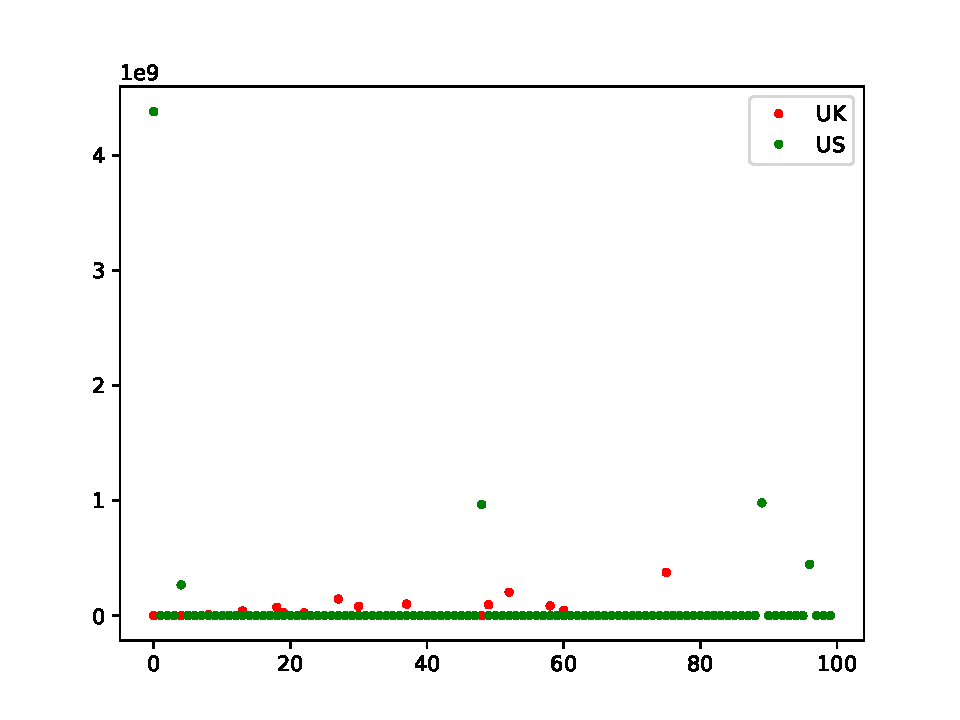
\includegraphics[width=1\textwidth,
  alt={Scatter plot of total Instagram likes for 100 celebrities, red dots for UK and green for US, on a linear vertical axis up to 4.4 billion. Nearly every point sits on the zero line; one US celebrity at the far left reaches 4.4 billion, two US points sit near 1 billion, and a handful of UK and US points lie between 0.1 and 0.5 billion.}]{rein1.pdf}
\caption{A regular (non-logarithmic) plot of celebrity ``likes.''}
\label{fig:rein1}
\end{figure}

The scatterplot is shown in Figure~\ref{fig:rein1}. It has limited use,
because there are a few uber-celebrities (Justin Bieber, \textit{etc.}) who
have far more ``likes'' than anyone else. Hence most people are crushed
against the bottom of the plot and we can't (say) compare the UK people with
the US people easily.

\index{scatter plot!logarithmic scale}

We can dramatically improve the readability and analyze-ability by plotting
the $y$ axis on a log scale. Just add this line before \texttt{plt.show()}:
\begin{Verbatim}[fontsize=\small,samepage=true,frame=single,framesep=3mm]
plt.yscale('log')
\end{Verbatim}

and voila, Figure~\ref{fig:rein2}. It's imperative that when you do this,
however, you remember that the $y$-axis no longer represents number-of-likes,
but log-number-of-likes.

\begin{figure}[ht]
\centering
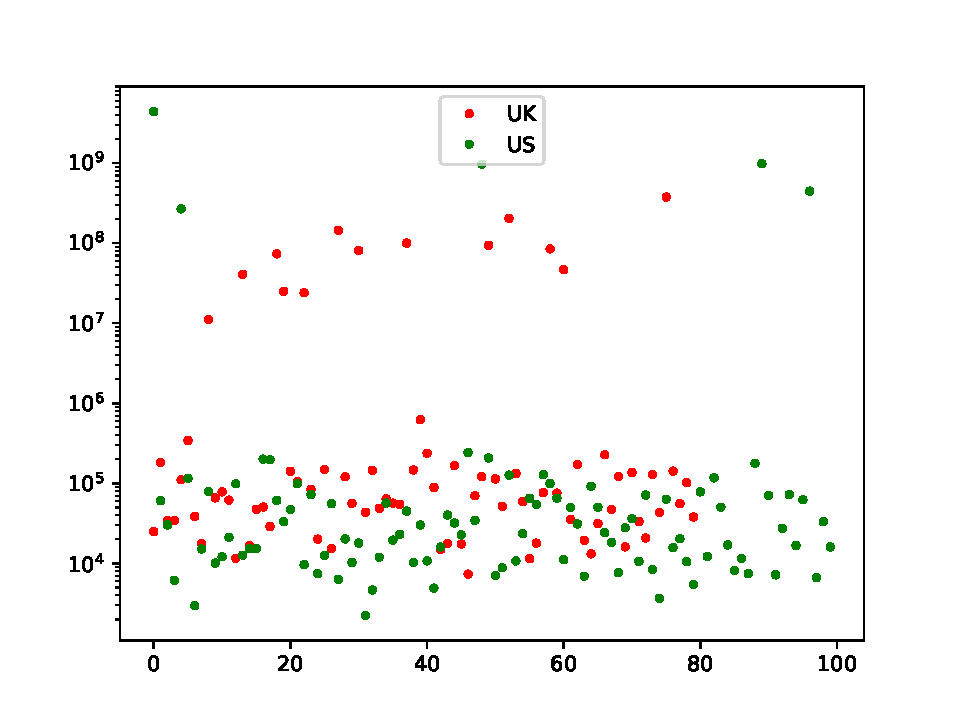
\includegraphics[width=1\textwidth,
  alt={The same celebrity likes on a logarithmic vertical axis from ten thousand to ten billion. The points now spread into a wide band mostly between ten thousand and a few hundred thousand likes, with about a dozen UK and US outliers between ten million and one billion, and the single US celebrity at about 4 billion at the top.}]{rein2.pdf}
\caption{A logarithmic plot of the same data from Figure~\ref{fig:rein1}.}
\label{fig:rein2}
\end{figure}

\index{relative vs.~absolute changes}
\index{absolute vs.~relative changes}
\index{stock prices}
\index{Stephen, Inc.}

\item \textbf{A semi-log plot shows \textbf{relative} (multiplicative) changes
instead of \textbf{absolute} (additive) changes.} Consider
Figure~\ref{fig:stock1}, whose (ordinary, not logarithmic) plot depicts a
fictional company's stock price over time. Two significant events occurred in
this company's history: one in April 2015 and the other in March 2017. Both
caused the stock's value to jump. Question: would you rather have bought stock
immediately before event A and sold it immediately after, or done the same
before/after B?

\begin{figure}[ht]
\centering
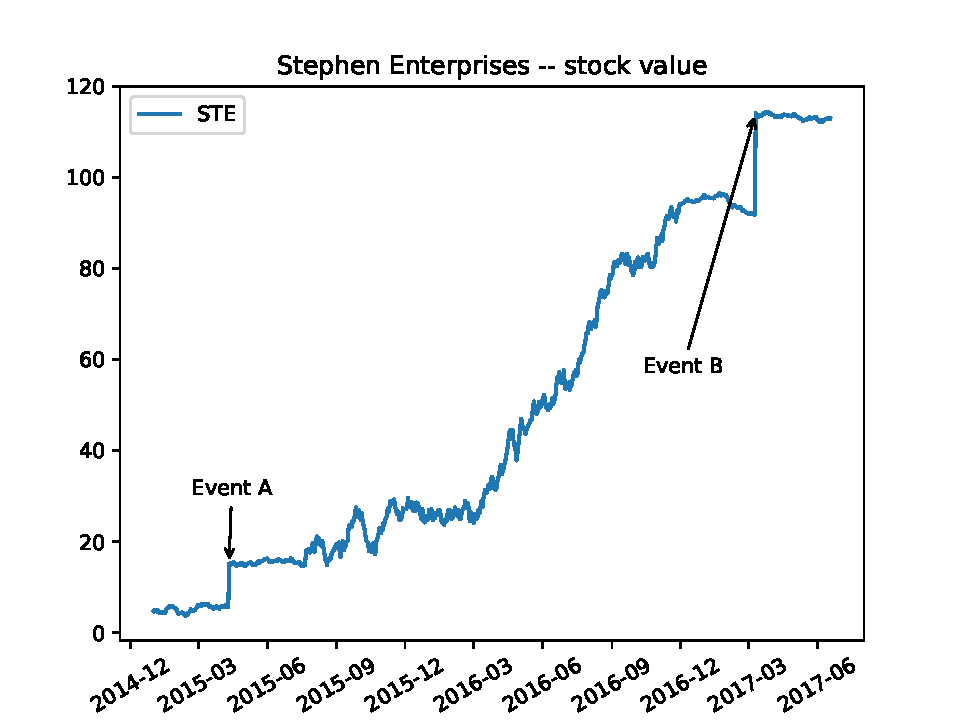
\includegraphics[width=0.8\textwidth,
  alt={Line plot titled Stephen Enterprises stock value, December 2014 to June 2017, price on a linear axis from 0 to 120. The line rises from about 5 to a plateau near 113. Two labeled jumps: Event A in early 2015 lifts the price from about 5 to 15, and Event B in early 2017 lifts it from about 92 to 113; between them the price climbs steadily through 2016.}]{stock1.pdf}
\caption{A regular (non-logarithmic) plot of a company's stock price.}
\label{fig:stock1}
\end{figure}

From Figure~\ref{fig:stock1}, it may look like event B is the better bet:
after all, it looks like the jump was higher. But this is an \textit{absolute}
distance: in other words, the total number of dollars per share jumped higher
for event B. But for something like an investment, you actually don't care
about this absolute number, but the \textit{relative} number. 

Look carefully at event A: before the jump, the stock was selling at about \$5
per share, and afterwards, at about \$15. This means that if you timed this
right, you \textit{tripled your money}! (Buy \$1000 worth of stock in April
2015, and you sell it for \$3000 the following day.) Compared to event B, this
is a way better deal. Consider that at event B, the stock went from \$90 to
\$110. Sure, \$20 is more than \$10 in absolute dollar terms, but if you
bought \$1000 worth of stock in March 2017 and sold it the following day,
you'd have sold it for \$$1000 \times \frac{110}{90} = $\$1222. Nice, but not
nearly the windfall of event A.

\index{semi-log plot}
For this reason, stocks and other investments are nearly always shown on a
semi-log plot, like the one in Figure~\ref{fig:stock2}. it has the advantage
that \textit{same-size increases on the (log) $y$ axis correspond to identical
\textit{relative} (multiplicative) increases of the stock.} In other words, if
the stock rises an inch somewhere on the plot, and it rises an inch somewhere
else, these represent equal gains for investors \textit{no matter how high the
stock value is in absolute terms.} Such is the magic of logs.

\index{windfall}

In this example, you can easily see from the semi-log plot that event A was a
bigger windfall for investors than event B.

\begin{figure}[ht]
\centering
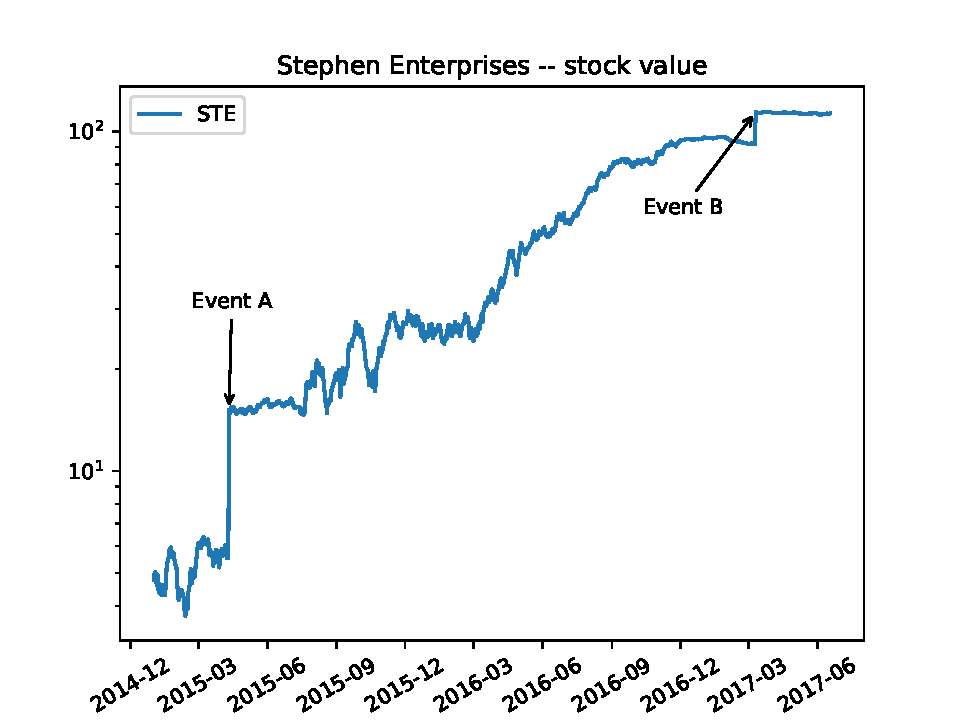
\includegraphics[width=0.8\textwidth,
  alt={The same stock price on a logarithmic vertical axis from about 5 to 120. The Event A jump in early 2015 now shows as the taller step, roughly tripling the price, while the Event B jump in early 2017 is a small step; the 2016 climb is a gentle upward curve.}]{stock2.pdf}
\caption{A semi-logarithmic plot of a company's stock price.}
\label{fig:stock2}
\end{figure}

\index{exponential relationship}
\index{power-law relationship}
\item \textbf{It reveals exponential and power-law relationships.} This
requires a little math to understand. Suppose we have two variables, $x$ and
$y$, and they are related according to something like this:
\begin{align*}
y = p \cdot e^{qx}
\end{align*}
where $p$ and $q$ are just numbers. For example,
\begin{align*}
y = 5.2 \cdot e^{2.96 x}
\end{align*}

Now if we plot $x$ vs $y$ on a standard plot, we get a curvy exponential
function that is very difficult for the human eye to distinguish from other
curvy functions. But suppose we plot not $y$, but the \textit{logarithm} of
$y$? 

Let's take the natural log ($\ln$) of both sides of the equation. Using our
properties from above, we get:

\begin{align*}
\ln y &= \ln (5.2 \cdot e^{2.96 x}) \\
&= \ln(5.2) + \ln(e^{2.96 x}) \\
&= 1.649 + 2.96 x \\
\end{align*}
This is just a linear equation with a slope ($m$) of 2.96 and a $y$-intercept
($b$) of 1.649. So plotting this relationship on a semi-log plot will give us
a straight line.

\index{rate of increase}

Why do we care? Because it turns out that exponential relationships like this
come up a lot in the world. One ubiquitous pattern is that of exponential
growth or decay: any time that \textit{the rate of increase of a quantity}
(like the number of new baby rabbits added to a rabbit population) is
proportional to \textit{the quantity itself} (the number of existing rabbits),
we have exponential growth. And any time that the rate of \textit{de}crease of
a quantity (like the number of mechanical parts that wear out) is proportional
to the quantity itself (the total number of mechanical parts owned by the
company), we have exponential decay.

\index{power-law relationship}
Another important kind of relationship is often mistaken for exponential
growth, but is emphatically \textit{not}. It's called a ``power-law''
relationship, and has caused much buzz in the scientific community over the
past decade or so. It occurs when we have a simple polynomial relationship:
\begin{align*}
y = p \cdot x^{q}
\end{align*}
where $p$ and $q$ are just numbers. For example,
\begin{align*}
y = 3.9 \cdot x^{-2.45}
\end{align*}

Again, some math: if we take the logarithm of both sides, we get:
\begin{align*}
\ln y &= \ln (3.9 \cdot x^{-2.45}) \\
\ln y &= \ln (3.9) + \ln (x^{-2.45}) \\
\ln y &= 1.361 -2.45 \ln (x) \\
\end{align*}
\normalsize

\vspace{-.25in}
If we plot not $y$ vs $x$, but $\ln y$ vs $\ln x$ (in other words, a
\textbf{log-log plot}, we will get a straight line. (You can see this by
mentally substituting your letter of choice for $\ln x$ and another letter of
your choice for $\ln y$. Now you have a plain old linear equation with a slope
of -2.45 and an intercept of 1.361.)

To see how the logarithmic plots reveal this, consider
Figure~\ref{fig:straightLines}, each of which is a plot of the same three
synthetic data sets. The blue points are linear in $x$, the red points are
exponential, and the green points are power-law (with an exponent of 6).

\begin{figure}[ht]
\centering
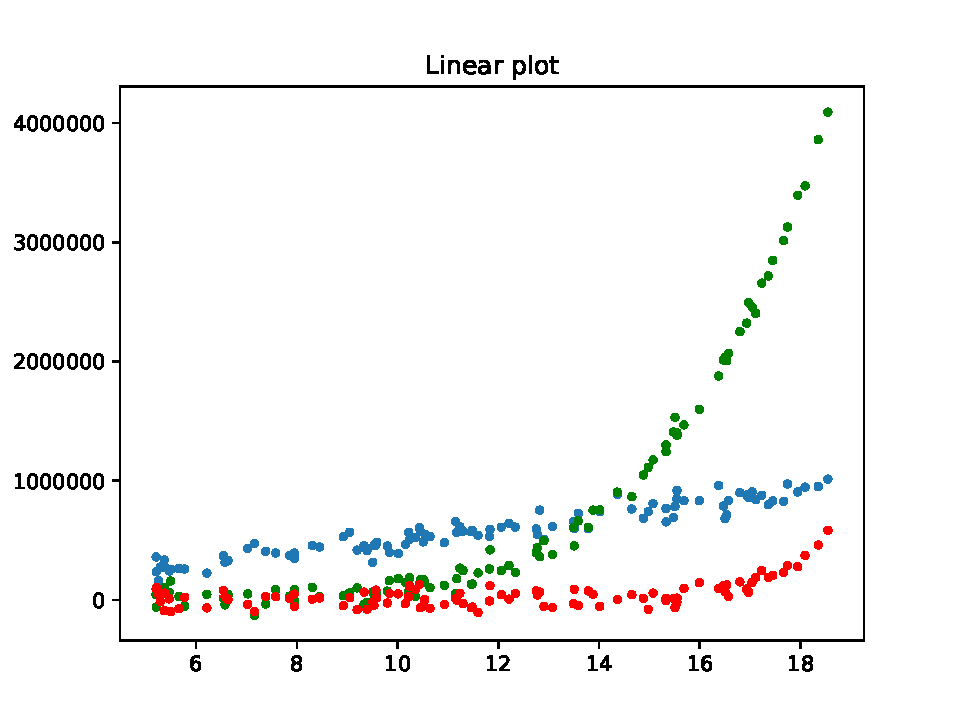
\includegraphics[width=0.6\textwidth,
  alt={Scatter plot titled Linear plot of three synthetic data sets over x from 5 to 18.5, linear vertical axis up to 4 million. Blue points rise slowly along a straight line from about 250,000 to 1 million; green points hug zero until x = 12 and then shoot up past 4 million; red points stay near zero the whole way, reaching only about 600,000 at the far right.}]{logplots1.pdf}
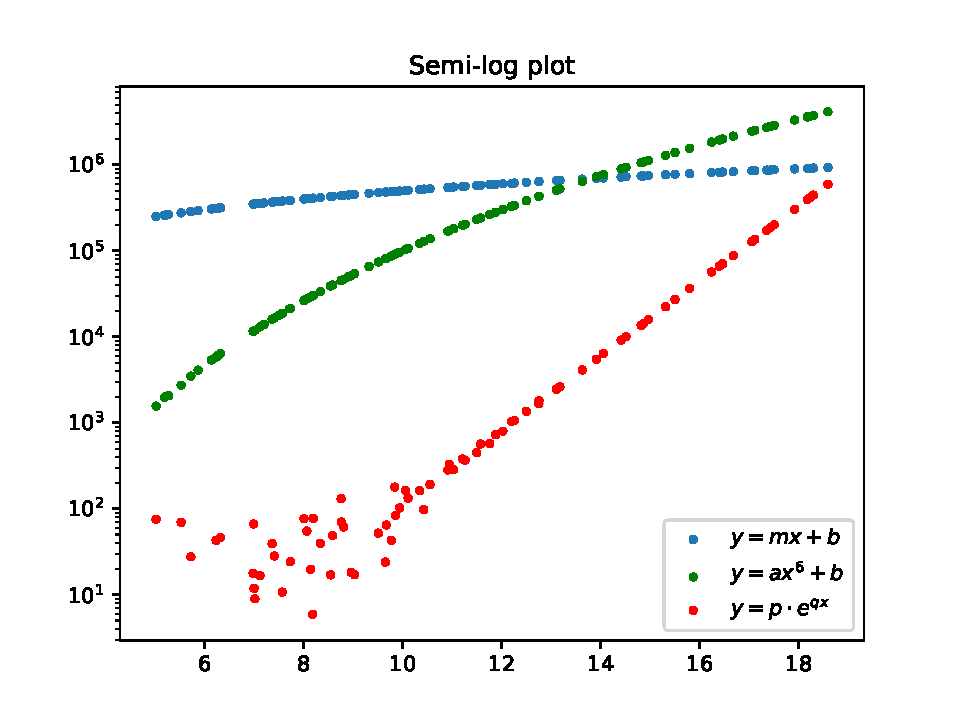
\includegraphics[width=0.6\textwidth,
  alt={Scatter plot titled Semi-log plot of the same three data sets, vertical axis logarithmic from 10 to 10 million, with a legend naming blue y = mx + b, green y = a times x to the sixth plus b, and red y = p times e to the qx. The red exponential points now form a straight line rising from about 10 to 600,000; the green power-law points form a concave-down curve; the blue linear points form a nearly flat, slightly rising curve.}]{logplots2.pdf}
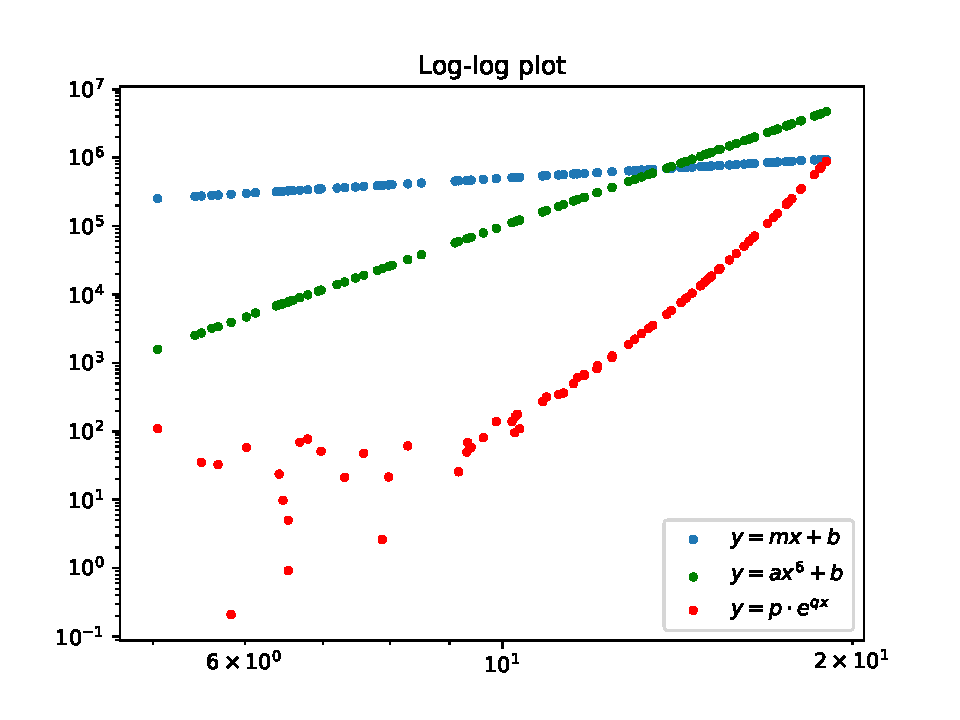
\includegraphics[width=0.6\textwidth,
  alt={Scatter plot titled Log-log plot of the same three data sets, both axes logarithmic. The green power-law points now form a straight line rising from about 1,500 to 5 million; the red exponential points curve upward ever more steeply; the blue linear points form a gently rising curve near the top.}]{logplots3.pdf}
\caption{A linear, semi-log, and log-log plot of the same three data sets:
blue (linear), red (exponential), and green (power-law).}
\label{fig:straightLines}
\end{figure}

In the linear plot, the blue points can be seen to be a straight line. In the
semi-log plot, the red points are. In the log-log plot, the green points are.
This is a powerful tool for recognizing these important kinds of relationships
at a glance.
\end{enumerate}            

\chapter{Accessing databases}

\index{database}
\index{DBMS}

``Database'' is a very loose term for ``a repository of information that can
be readily accessed.'' When we use that term in Data Science, we mean a data
source that is managed by a piece of software called a \textbf{DBMS}, or
\textbf{database management system}. (True, plain-old lists, dictionaries, or
Pandas \texttt{DataFrame}s are also ``repositories of information that can be
accessed,'' but when we use the term \textbf{database} we're not talking about
that.)

There are principally two reasons to learn how to access data from databases:

\begin{itemize}
\itemsep.1em
\item Sometimes, our data is simply available in that form only. We may want
to import it into Python/Pandas and deal with it using the techniques from the
first half of the semester, but in order to get it in there, we need to
(briefly) interface with the database and issue the proper commands.
\item Sometimes, our data is just flat \textit{big}. There's a limit to how
much data Spyder can store in memory and deal with on the spot. Suppose
you had to analyze all the eBay transactions over the past two years? Or all
the tweets made in the world over the last month? That stuff can't remotely
fit in your system's memory. Hence, we have to access it through a database
which will manage the sheer size and scope for us, and work with it a little
at a time.
\end{itemize}

\section{Two kinds of databases}

\index{relational database}
\index{NoSQL database}

There are essentially two kinds of databases in the world:
\textbf{relational}, and \textbf{NoSQL}.

\index{table!relational database}
\index{SQL}
\index{RDBMS}

Previously this semester, we've worked with data spread across multiple
\texttt{DataFrame}s that we need to join together in some way. This structure
is extremely common, so much so that most of traditional database schema theory
is based directly on it. A \textbf{relational database} is a repository of
information in which the data is stored in \textbf{tables} (a table is pretty
much \textit{exactly} a \texttt{DataFrame} in spirit), and on which the
language \textbf{SQL}\footnote{Some people pronounce the acronym SQL as the
three letters ``ess-queue-ell,'' and others as the word ``sequel.'' Either one
is acceptable (I do the former).} can be used to query it and manipulate it. A
software system that enables a user to create and work with relational
databases is called an \textbf{RDBMS}, or \textbf{relational database
management system}.

\index{Oracle}
\index{Sybase}
\index{Microsoft SQL Server}
\index{MySQL}
\index{MariaDB}
\index{PostgreSQL}
\index{Codd, Ted}

There are many, many RDBMS's out there: Oracle, Sybase, Microsoft SQL Server,
MySQL, MariaDB, PostgreSQL, and literally dozens of others. They all work in
very much the same way: they store data in tables, and they are manipulated via
SQL. Ever since Ted Codd invented the relational model in 1970, this
organizational paradigm has proven to be so powerful and computationally
efficient that it has dominated the database world. Only recently have some
alternate paradigms gained some traction (so-called ``NoSQL'' databases), but
even so, the majority of the world's structured data is all in relational
databases of some sort.

\index{Cassandra}
\index{MongoDB}
\index{Redis}
\index{Neo4j}
\index{key-value pair}
\index{graph (network)}

Relational DBMS's are much more similar to each other than NoSQL systems are to
each other. The wide variety of NoSQL DBMS's (Cassandra, MongoDB, Redis, Neo4j,
\textit{etc.}) means that learning how to use one doesn't give you much
knowledge about how to use one of the others. Some store key/value pairs;
others store objects and binary data; some store information as a graph
(network). Part of the great power of the relational model is that SQL has
proven to be a common, flexible, broadly-applicable query language that many
different vendors have adopted and which suits many data needs.

\section{SQLite}

\index{SQLite}
\index{RDBMS}

SQLite is a really slim, trim RDBMS that stores all of its data \textit{in a
single file.} When you work with SQLite (or any RDBMS), though, you don't think
in terms of files, but in terms of tables. The fact that the tables are stored
in file(s) in some strange format is invisible to you as the user of the data,
and this is in fact one of the great powers of the relational model: separating
the conceptual data from the storage implementation.

\subsection{Interfacing to SQLite}

\index{connect@\texttt{connect()} (SQLite)}

``\textbf{Connecting}'' to a relational database basically means establishing a
communication path over which you can talk SQL. In Python, this is pretty easy:

\begin{Verbatim}[fontsize=\small,samepage=true,frame=single,framesep=3mm]
import sqlite3

conn = sqlite3.connect('my_local_file.db')
\end{Verbatim}
\label{connectSqlite}

\index{extension (filename)}
\index{db file@\texttt{.db} file}

As indicated, SQLite-compatible files typically have a \texttt{.db} extension
(for ``database.'')

\index{query (database)}

The return value from \texttt{connect()} that we're calling \texttt{conn} is
``a connection to the database.'' We'll use it every time we want to perform an
\textbf{SQL query}. SQL is a new language, but it's not nearly as complex as
something like Python because it's not a programming language, but a
\textbf{query language}. You don't write entire programs in it; you merely
specify queries in it. This means that the range of things you can do in SQL is
much more restricted, and hence the language is easier to learn.

\subsection{Browsing the tables}

\index{read\_sql@\texttt{read\_sql()} (Pandas)}
\index{table!relational database}

The first thing you'll normally want to do is figure out which tables exist in
the database. You can run this command:

\index{sqlite\_master@\texttt{sqlite\_master}}
\label{sqlite_master}
\index{SELECT statement@\texttt{SELECT} statement (SQL)}
\index{FROM clause@``\texttt{FROM}'' clause (SQL)}

\begin{Verbatim}[fontsize=\footnotesize,samepage=true,frame=single,framesep=3mm]
print(pd.read_sql(
    "SELECT name FROM sqlite_master WHERE type='table'", conn))
\end{Verbatim}

to find out. If this were the output:

\begin{Verbatim}[fontsize=\small,samepage=true,frame=leftline,framesep=5mm,framerule=1mm]
          name
0        songs
1       albums
2      artists
3       labels
\end{Verbatim}

that would tell us that the SQLite database has four tables in it, named
\texttt{songs}, \texttt{albums}, \texttt{artists}, and \texttt{labels}. Each
one can be queried using SQL statements, or simply imported wholesale into a
Pandas \texttt{DataFrame} (see below).

\section{Querying the database}

\index{read\_sql@\texttt{read\_sql()} (Pandas)}

By far the most common thing you'll do with a relational database like SQLite
is execute an SQL query, and get a \texttt{DataFrame} back:

\begin{Verbatim}[fontsize=\small,samepage=true,frame=single,framesep=3mm]
df_name = pd.read_sql("YOUR SQL QUERY GOES HERE", conn)
\end{Verbatim}

\index{embedded statement@``embedded'' statement}

The string inside the call to \texttt{pd.read\_sql()} is called ``an embedded
SQL statement.'' This means we have code in one language (SQL) ``embedded''
inside another (Python). Do not be alarmed at this.


\subsection{The easy case: inhaling an entire table}
\index{the easy case}
\label{easy1}

Now \textit{if} the data is small enough to load into memory, you don't need to
know much SQL at all. You can simply use this one-liner:

\index{SELECT statement@\texttt{SELECT} statement (SQL)}
\index{*@\texttt{*} (splat) (SQL)}
\index{FROM clause@``\texttt{FROM}'' clause (SQL)}

\begin{Verbatim}[fontsize=\small,samepage=true,frame=single,framesep=3mm]
df = pd.read_sql("SELECT * FROM table_name", conn)
\end{Verbatim}

This reads one of the database's tables (whose names you learned from the
command in Section~\ref{sqlite_master}) into a new, fully-fledged
\texttt{DataFrame}, with column names, a reasonable guess at their types,
\textit{etc.} 

That's literally all you need to know about working with a (smallish) SQLite
database. Just to connect to it, get all the table names, read each one into a
\texttt{DataFrame}, and continue in Pandas Land, forgetting all about SQLite.
You can then leverage all the knowledge you've learned up to this point. Bingo!


\subsection{The harder case: more complex SQL}

\index{SQL}

Sometimes, however, the data is too large to do this. So it's worth learning a
little SQL so you can make the RDBMS do some of the heavy lifting, and give you
trimmed results for your Python program to work with.

\index{SELECT statement@\texttt{SELECT} statement (SQL)}

The workhorse is the SQL \texttt{SELECT} statement. Here are some common
variants:

\index{*@\texttt{*} (splat) (SQL)}
\begin{itemize}
\itemsep1em
\item To compute the \textit{number} of rows, or individual values, without
returning the entire result, use \texttt{COUNT(*)}, \texttt{MAX()},
\texttt{MIN()}, \textit{etc.}:

\index{COUNT@\texttt{COUNT()} (SQL)}
\index{MAX@\texttt{MAX()} (SQL)}
\index{MIN@\texttt{MIN()} (SQL)}
\index{FROM clause@``\texttt{FROM}'' clause (SQL)}
\begin{BVerbatim}[fontsize=\small,samepage=true,frame=single,framesep=3mm,bgcolor=AliceBlue]
SELECT COUNT(*) FROM table_name
SELECT MAX(col1) FROM table_name
\end{BVerbatim}

\index{LIMIT clause@``\texttt{LIMIT}'' clause (SQL)}
\item To get only the first few rows (similar to Pandas' \texttt{.head()}
operation) tack on a ``\texttt{LIMIT}'' expression:

\begin{BVerbatim}[fontsize=\small,samepage=true,frame=single,framesep=3mm,bgcolor=AliceBlue]
SELECT * FROM table_name LIMIT 10
\end{BVerbatim}

\item To get only certain columns, change the ``\texttt{*}'' to a
comma-separated list of column names:

\begin{BVerbatim}[fontsize=\small,samepage=true,frame=single,framesep=3mm,bgcolor=AliceBlue]
SELECT col1 FROM table_name
SELECT col1,col2,col3 FROM table_name LIMIT 10
\end{BVerbatim}

\index{WHERE clause@``\texttt{WHERE}'' clause (SQL)}
\item To get only certain rows, add a ``\texttt{WHERE} clause'' after the table
name:

\begin{BVerbatim}[fontsize=\footnotesize,samepage=true,frame=single,framesep=3mm,bgcolor=AliceBlue]
SELECT * FROM table_name WHERE col1==val1
SELECT col2 FROM table_name WHERE col1==val1 AND col2>val2
SELECT c1,c2 FROM t WHERE c1==val1 AND NOT c2>val2 LIMIT 10
\end{BVerbatim}

(The usual boolean operations work with keywords \texttt{AND}, \texttt{OR},
and \texttt{NOT}, and parentheses for grouping.)

\index{IN keyword@``\texttt{IN}'' keyword (SQL)}
\item The ``\texttt{IN}'' keyword can be useful in a \texttt{WHERE} clause
for querying membership in a set:

\begin{BVerbatim}[fontsize=\small,samepage=true,frame=single,framesep=3mm,bgcolor=AliceBlue]
SELECT * FROM table_name WHERE col1 IN (val1,val2)
SELECT col1,col2 FROM table_name WHERE col1==val1 AND
            NOT col2 IN (val1,val2,val3) LIMIT 10
\end{BVerbatim}

\index{unique@unique rows (with \texttt{DISTINCT})}
\index{DISTINCT@\texttt{DISTINCT} (SQL)}
\item To get only unique rows (like Pandas' \texttt{.drop\_duplicates()}
gives) use the word \texttt{DISTINCT} before the column names:

\begin{BVerbatim}[fontsize=\small,samepage=true,frame=single,framesep=3mm,bgcolor=AliceBlue]
SELECT DISTINCT * FROM table_name
SELECT col1,col2 FROM table_name WHERE NOT col1 IN
            (val1,val2,val3) OR col2!=val4 LIMIT 5
\end{BVerbatim}

\index{DISTINCT@\texttt{DISTINCT} (SQL)}
\index{COUNT@\texttt{COUNT()} (SQL)}
The \texttt{DISTINCT} option is useful in conjunction with \texttt{COUNT()}:

\begin{BVerbatim}[fontsize=\small,samepage=true,frame=single,framesep=3mm,bgcolor=AliceBlue]
SELECT COUNT(DISTINCT col1) FROM table_name
\end{BVerbatim}

\index{ORDER BY@\texttt{ORDER BY} (SQL)}
\item You can have SQLite do sorting with ``\texttt{ORDER BY}'':

\index{DESC@\texttt{DESC} (``descending'') (SQL)}
\begin{BVerbatim}[fontsize=\small,samepage=true,frame=single,framesep=3mm,bgcolor=AliceBlue]
SELECT * FROM table_name ORDER BY col1
SELECT DISTINCT c1,c2 FROM table_name WHERE c1==val1
            ORDER BY c2,c1 DESC LIMIT 5
\end{BVerbatim}

As you can see, you can sort on multiple columns, and sort in reverse order
with the \texttt{DESC} keyword.

\index{GROUP BY@\texttt{GROUP BY} (SQL)}
\index{groupby@\texttt{.groupby()} (Pandas)}
\item SQL supports a ``GROUP BY'' operation very much like Pandas'
\texttt{.groupby()} method:

\begin{BVerbatim}[fontsize=\small,samepage=true,frame=single,framesep=3mm,bgcolor=AliceBlue]
SELECT col1,count(*) FROM table_name GROUP BY col1
SELECT col1,max(col2) FROM table_name WHERE col3==val1
            GROUP BY col2 ORDER BY col1 DESC LIMIT 5
\end{BVerbatim}

\index{join!JOIN@\texttt{JOIN} (SQL)}
\item Finally, to do a merge/join operation, use the \texttt{JOIN} keyword:

\begin{BVerbatim}[fontsize=\small,samepage=true,frame=single,framesep=3mm,bgcolor=AliceBlue]
SELECT * FROM table_1 join table_2 ON col1==col2
SELECT c1,c2 FROM t1 join t2 ON t1.x==t2.q
            WHERE c2>val1 LIMIT 5
\end{BVerbatim}

The \texttt{JOIN} keyword supports \texttt{LEFT}, \texttt{RIGHT}, and
\texttt{OUTER} options.

\end{itemize}

\index{Oracle}
\index{Sybase}
\index{Microsoft SQL Server}
\index{MySQL}
\index{MariaDB}
\index{PostgreSQL}
\index{Informix}

There are many, many other options as well. See the online documentation at
\url{https://www.sqlite.org/docs.html}. Again, one of the great things about
SQL is that with the exception of the initial commands to connect and to list
all table names (p.~\pageref{sqlite_master}), \textit{all relational databases
use essentially identical syntax.} So if you ever need to query an Oracle,
Sybase, Informix, MySQL, PostgreSQL, or SQL Server database, you'll discover
that everything in this section applies nearly identically.

       

\chapter{Screen scraping (1 of 2)}
\label{ch:screenScraping1}

\index{worst of all possible worlds}

Welcome to the worst of all possible worlds\footnote{Actually, the
\textit{second}-worst; the very worst is when the data you seek isn't even in
electronic form at all.}: when the data you want to analyze is on a
human-readable but machine-unfriendly website somewhere. It's there, you can
see it...but getting it from a pretty web page into a Pandas \texttt{DataFrame}
is a non-trivial proposition.

Usually this situation occurs when the provider of the data, and the designer
of the website, didn't envision anyone using the data for any purpose other
than viewing it through the website itself. Sometimes there is another reason:
that the organization wanted to deliberately make this operation difficult so
that you \textit{couldn't} easily use it for other purposes. Either way,
though, as long as the data is accessible and visible through your browser, it
is at least theoretically extractable into the form we need to do our magic.

\section{HTML}
\index{HTML}
\index{render (a web page)}

(Most) web pages look snazzy and colorful when you view them: the word ``code''
doesn't jump immediately to mind. When you load a web page, though, what you're
actually getting from the server you specify is a plain-text file written in a
language called \textbf{HTML}, or \textbf{hypertext markup language}. It
consists of a combination of content and formatting/structural commands (or
``markup'') to instruct the browser how to \textbf{render} the page.
(``Rendering'' a page means ``interpreting all that HTML formatting stuff and
actually presenting a pretty page formatted the way it specifies.)

The first thing to be aware of is that HTML is \textit{not} a programming
language. (That is, you can't write a program in it.) It's strictly a
formatting syntax for specifying how text and graphical elements should be laid
out. If you ever ask someone whether they've done computer programming, and
they say, ``yeah, I've done programming in HTML,'' you know they're lying.

\index{JSON}
\index{CSV file}
\index{hierarchical data}
\index{tree}

The second thing to know is that it is \textit{hierarchical}, not flat. This
makes it more like JSON than CSV. Even though every HTML file is a single
sequence of characters, it encodes a tree-like structure in which elements can
exist inside other elements, which can exist inside other elements,
\textit{etc.}, with no limit to the amount of nesting.

\index{element (HTML)}
\index{tag (HTML)}
\index{wakkas (angle brackets)}
\index{<>@\texttt{<>} (wakkas)}

\index{title@\texttt{<title>} (HTML tag)}

The basic building block of HTML is the \textbf{element}, which is delimited by
starting and ending \textbf{tags}. Tags are key words, most of which indicate
something structural or stylistic, enclosed in wakkas (``\texttt{< ... >}'').
The ending tag has a slash (``\texttt{/}'') immediately before the keyword,
showing that it matches the corresponding opening tag. So one pair of starting
and ending tags might be ``\texttt{<title>}'' and ``\texttt{</title>}''.

Note that the entire contents of the \textit{element} is (1) the starting tag,
(2) the ending tag, and (3) \textit{everything in between}, which could be
text in addition to other elements.

\subsection{An example HTML file}

\index{html@\texttt{<html>} (HTML tag)}
\index{head@\texttt{<head>} (HTML tag)}
\index{body@\texttt{<body>} (HTML tag)}
\index{root node (of an HTML file)}

Figure~\ref{fig:allAboutStephen} shows a very simple, but complete, example.
Lots going on there. The first way to get your bearings is to start visually
lining up starting tags with their corresponding ending tags and perceive the
structure. Notice that this entire page begins with ``\texttt{<html>}'' and
ends with ``\texttt{</html>}''. This is in essence the ``root node'' of the
page's entire hierarchical tree\footnote{I'm using the term \textbf{tree} here
in much the same way as the \textbf{decision tree}s from volume I of this
series. Remember that they start at the top with a \textbf{root}, and branch
out wider and wider as they are drawn down the page.} It has two immediate
``children'': a \texttt{head} element, and a \texttt{body} element. Each of
those have starting and ending tags as well. Inside the \texttt{head} element
is a \texttt{title} element, \textit{etc.}

\begin{figure}
\begin{Verbatim}[fontsize=\scriptsize,samepage=true,frame=lines]
<html>
<head>
    <title>All About Stephen</title>
    <style>
        img { width:150px; }
        td { border-width:1px; }
    </style>
</head>
<body>
<h1>Stephen Davies, Esquire</h1>

<p>Deep in the bowels of
<a href="http://buildings.umwblogs.org/james-farmer-hall/">James Farmer
Hall</a> resides a carbon-based life form known to outsiders only as
<b>Stephen</b>. This mysterious being fulfills several roles <u>not</u>
widely known to humankind.</p>

<p><i>Some</i> of these functions are delineated below. Please memorize
them and then immediately destroy this page upon reading it.</p>

<h2>Areas of operation</h2>

<table border=2 cellpadding=15>
    <tr><td class="pic"><img src="http://clipart.com/prof.jpg" width=200 />
        </td>
        <td class="role">College professor</td>
        <td class="description">Stephen teaches computer science and data
    science to willing undergraduates, shaping them into the heroes of
    tomorrow.</td>
        <td><ul><li>Super rewarding</li>
            <li>Exciting</li>
            <li>Ever-changing</li>
            <li>Fun</li></ul></td>
        <td><b>50%</b> of total time</td>
    </tr>
    <tr><td class="pic"><img src="http://clipart.com/dad.png" width=200 />
        </td>
        <td class="role">Dad</td>
        <td class="description"> With a wife, three teenagers, and two cats
        (one of whom throws up a lot), Stephen's home life is a constant
        source of love, anxiety, and Hallmark moments.</td>
        <td><ul><li>Amazing</li>
            <li>Loving</li>
            <li>Complicated</li>
            <li>Surprising</li></ul></td>
        <td><b>30%</b> of total time</td>
    </tr>
    ...
</table>
</body>
</html>
\end{Verbatim}
\caption{A sample HTML page.}
\label{fig:allAboutStephen}
\end{figure}

\index{h1@\texttt{<h1>}, \texttt{<h2>}, ... (HTML tags)}
\index{td@\texttt{<td>} (HTML tag)}
\index{tr@\texttt{<tr>} (HTML tag)}
\index{b@\texttt{<b>} (HTML tag)}
\index{i@\texttt{<i>} (HTML tag)}
\index{u@\texttt{<u>} (HTML tag)}
\index{table@\texttt{<table>} (HTML tag)}

As you can guess, each of these tags is interpreted by the browser to mean a
particular kind of structure/formatting. ``\texttt{h1}'' means ``top-level
heading'' which in practicality means ``render it in a large font, with some
extra space around it.'' The ``\texttt{b}'' element means to put something in
boldface. The ``\texttt{table}'' element means to construct a table-like
structure, with rows (``\texttt{tr}'') and cells within rows (``\texttt{td}'').
\textit{Etc.} HTML is in general a big mess of things that are supposed to
indicate structure (like \texttt{table} and \texttt{h2}) and things that
specify specific formatting (like \texttt{i} and \texttt{u}). All of this is
eminently look-up-able online.


\index{attribute!of an HTML element}
\index{img@\texttt{<img>} (HTML tag)}

Some starting tags (not ending) contain additional information called
\textbf{attributes}. You can see this with the \texttt{a} and \texttt{img}
tags from the example:

\vspace{-.15in}
\begin{Verbatim}[fontsize=\scriptsize,samepage=true,frame=lines]
<a href="http://buildings.umwblogs.org/james-farmer-hall/">Farmer Hall</a>
\end{Verbatim}
\vspace{-.15in}

\index{a@\texttt{<a>} (HTML tag)}
\index{attribute!of an HTML element}
\index{key-value pair}

The \texttt{a} tag stands for ``anchor'' and is the most common way of
embedding a hyperlink (which you can click on to go to another page) in a
document. Note that the words that will appear in the page are the
\textbf{contents} of the element, not part of the tag itself. The tag, in
addition to the required ``\texttt{a}'' has a key/value pair where the key is
the string \texttt{href} and the value is the URL the user will be directed to
if they click on the link. This key/value pair is called an
\textbf{attribute}.

\vspace{-.15in}
\begin{Verbatim}[fontsize=\footnotesize,samepage=true,frame=lines]
<img src="http://clipart.com/prof.jpg" width=200 />
\end{Verbatim}
\vspace{-.15in}

In the \texttt{img} example, we have \textit{two} attributes: one for the
filename of the image, and the other for some specific formatting suggestions
(in this case, a width of 200 pixels). An element can have many different
attributes, in any order.

\index{img@\texttt{<img>} (HTML tag)}
\index{element (HTML)}
\index{tag (HTML)}

(By the way, the sharp-eyed reader may have noticed something else odd about
the \texttt{img} example, above: an extra slash before the ending
``\texttt{>}''. This is an HTML shorthand for ``starting and ending the element
all within a single tag, since it has no content anyway.'' Whenever you have
something of the form ``\texttt{<x></x>}'' you can replace it with the
equivalent ``\texttt{<x/>}'' to save typing and file size.)

Lastly, I'll point out that near the top of this example, there's a bunch of
stuff which looks a bit visually jarring; it doesn't look like HTML. And it's
not. I'm referring to this:

\vspace{-.15in}
\begin{Verbatim}[fontsize=\footnotesize,samepage=true,frame=lines]
    <style>
        img { width:150px; }
        td { border-width:1px; }
    </style>
\end{Verbatim}
\vspace{-.15in}

\index{CSS}

This code is called \textbf{CSS} (or \textbf{Cascading Style Sheets}) which is
sort of a companion technology to HTML to give additional formatting control.
(Originally, HTML was supposed to strictly delineate document
\textit{structure}, and CSS could then be used to specify the formatting of
that structure. This strict separation of concerns, which was a good idea, has
gotten very muddy in the intervening years, however.)

The whole thing, once rendered, looks something like this:

\begin{center}
\label{stephenpage}
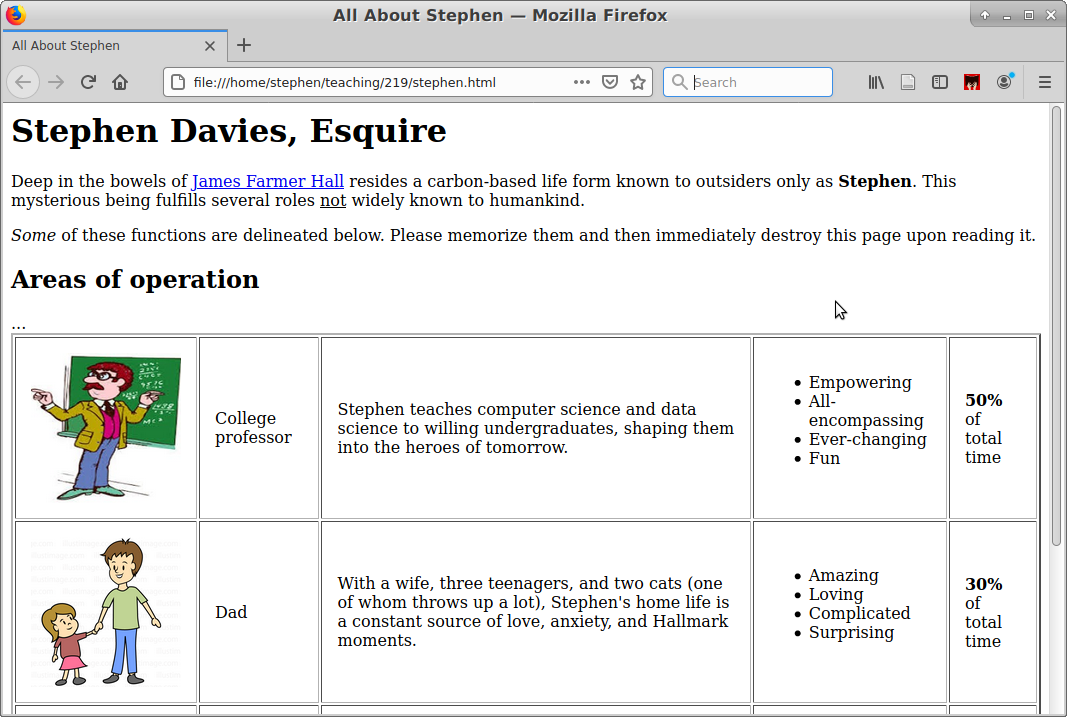
\includegraphics[width=0.9\textwidth]{stephenpage.png}
\end{center}

\section{The easy case: reading from \texttt{<table>}s}

\index{the easy case}
\label{easy2}
\index{screen scraping}

From the point of view of Data Science, we don't care very much about all this
formatting stuff. To us, it's clutter. On the page is some important data we'd
like to analyze, and the goal is to sift through all this HTML and CSS crapola
looking for it and extracting it. This is called by the evocative term
``\textbf{screen scraping}.''

\index{table@\texttt{<table>} (HTML tag)}
\index{table!HTML element}

Now just like with relational databases (recall p.~\pageref{easy1}), there's
both an easy scenario and more challenging ones. The more challenging ones
we'll postpone until the next chapter. The easy one is when the data you want
to scrape \textit{is all inside \textbf{HTML tables}}. 

\index{read\_html@\texttt{read\_html()} (Pandas)}

An HTML table is the contents between an opening \textbf{<table>} tag and its
corresponding \textbf{</table>} tag. Look carefully again at
Figure~\ref{fig:allAboutStephen} on p.~\pageref{fig:allAboutStephen}.
\textit{If} the information we care about scraping is all inside the ``areas of
operation'' table (which begins about half-way down the page; squint until you
see the word \texttt{table}), then we're in the easy case, thank heavens. We
can use Pandas' \texttt{read\_html()} function as follows:

\vspace{-.1in}
\begin{Verbatim}[fontsize=\footnotesize,samepage=true,frame=single,framesep=3mm]
the_tables = pd.read_html("http://theURLtoTheWebpage.html")
\end{Verbatim}
\vspace{-.1in}

\index{URL}
\index{network connection}
\index{directory (folder)}
\index{folder}
\index{extension (filename)}

\index{allAboutStephen@\texttt{allAboutStephen.html}}

\label{downloading}

This function takes just one argument: the \textbf{URL} of the page we want to
scrape. (A URL -- which stands for Uniform Resource Locator -- is another word
for a web page's address, or ``link.'') Sometimes you'll find it more
convenient to first download the page to your local computer, so that you're
not dependent on a network connection (and latency) while you're working on
scraping it. This will normally put a \texttt{.html} (or \texttt{.htm}) file on
your computer, which you can store in the same directory/folder as your
\texttt{.py} file, just as you do with \texttt{.csv} or \texttt{.db} files.
You'll then pass the simple filename (like ``\texttt{allAboutStephen.htm}'') as
the argument to \texttt{read\_html()}.

The return value of this function is \textit{a list of \texttt{DataFrame}s, one
for each \texttt{<table>} on the page.} Read that sentence once again slowly.
In particular, note that the return value is not \textit{a} \texttt{DataFrame},
which many students seem to expect. This is of course because the web page may
well contain \textit{multiple} \texttt{<table>}s, and therefore
\texttt{read\_html()} would need to return multiple \texttt{DataFrame}s.

\index{allAboutStephen@\texttt{allAboutStephen.html}}

Let's try this approach with \texttt{allAboutStephen.html}:

\begin{Verbatim}[fontsize=\small,samepage=true,frame=single,framesep=3mm]
the_tables = pd.read_html(
    "http://stephendavies.org/allAboutStephen.html")
print(len(the_tables))
\end{Verbatim}
\vspace{-.2in}

\begin{Verbatim}[fontsize=\small,samepage=true,frame=leftline,framesep=5mm,framerule=1mm]
1
\end{Verbatim}

There is apparently only one \texttt{<table>} on the page. Let's put it in its
own variable (``\texttt{areas}'' for ``Areas of operation'') and take a look at
it:

\begin{Verbatim}[fontsize=\small,samepage=true,frame=single,framesep=3mm]
areas = the_tables[0]
print(areas)
\end{Verbatim}
\vspace{-.2in}

\begin{Verbatim}[fontsize=\small,samepage=true,frame=leftline,framesep=5mm,framerule=1mm]
    0  ...                  4
0 NaN  ...  50% of total time
1 NaN  ...  30% of total time
2 NaN  ...  10% of total time
3 NaN  ...   5% of total time
4 NaN  ...   5% of total time

[5 rows x 5 columns]
\end{Verbatim}

\index{NaN@\texttt{NaN} (``not a number'')}

This is a bit confusing at first, for several reasons. One is that the columns
don't have names, as we're used to -- just numbers. Another is that most of the
information is omitted from the display (with just ``\texttt{...}''
placeholders). Another is that the first column is entirely \texttt{NaN}
values\footnote{The value \texttt{NaN}, you'll recall, stands for ``not a
number.'' But that phrase is misleading here. Of \textit{course} the value is
not a \textit{number}: why would we expect text on a web page to necessarily be
a number? Really it means ``not a value Python could do anything with.''}.

\pagebreak
The root causes of these conundrums are as follows:

\begin{compactenum}

\item The \texttt{DataFrame} columns don't have names because HTML
\texttt{<table>}s often don't have header cells (delimited with \texttt{<th>}
cells in the first \texttt{<tr>} row), and so \texttt{read\_html()} has no idea
what to name the columns.

\item Most columns are omitted from the \texttt{print()} output because they're
just too long to fit. (Look at p.~\pageref{stephenpage}: that third column has paragraphs in it.)

\item The first column has \texttt{NaN}s because the first column of the
\texttt{<table>} has images in it, not text (again see
p.~\pageref{stephenpage}).

\end{compactenum}

We can \textit{give} the \texttt{DataFrame} meaningful column names with:

\begin{Verbatim}[fontsize=\small,samepage=true,frame=single,framesep=3mm]
areas.columns = ['pic','role','description','adjectives',
    'allocation']
\end{Verbatim}

and we can get rid of the columns we don't care about (the image, and perhaps
the descriptions) with a Pandas operation:

\begin{Verbatim}[fontsize=\small,samepage=true,frame=single,framesep=3mm]
areas = areas[['role','adjectives','allocation']]
\end{Verbatim}

Now we can see better what's going on:

\begin{Verbatim}[fontsize=\small,samepage=true,frame=single,framesep=3mm]
print(areas)
\end{Verbatim}

\vspace{-.2in}

\begin{Verbatim}[fontsize=\scriptsize,samepage=true,frame=leftline,framesep=3mm,framerule=1mm]
             role                        adjectives          allocation
College professor   Empowering  Important  Fun  ...   50% of total time
Dad                            Amazing Fun Impor...   30% of total time
Kids Club Leader    Cute  Exhausting  Character-...   10% of total time
Secret Agent        Thrilling  High-impact  Dang...    5% of total time
Jedi Master         Important  Thrilling  Challe...    5% of total time
\end{Verbatim}

\subsection{Some text cleaning stuff}

At this point, we're out of screen-scraping-land and into ordinary-Python land.
What we do next depends on what we want to analyze. One interesting question I
could imagine asking is: ``how much of Stephen's total time does he spend doing
`fun' things? `important' things? `exhausting' things?

\index{adjectives@\texttt{adjectives}}
\index{ul@\texttt{<ul>} (HTML tag)}
\index{li@\texttt{<li>} (HTML tag)}

To do this, we'll have to deal with that messy \texttt{adjectives} column. I
say it's ``messy'' because all Pandas knew to do was take each bulleted list
-- comprised of a \texttt{<ul>} element (``unordered list'') and nested
\texttt{<li>} elements (``list elements'') -- and concatenate all the contents
into a single string.

My strategy to dealing with it is to split these up, putting each role's
adjective in its own row of a new table that looks like this:

\begin{Verbatim}[fontsize=\small,samepage=true,frame=leftline,framesep=5mm,framerule=1mm]
                   role           adjective
      College professor          Empowering
      College professor           Important
                    Dad             Amazing
       Kids Club Leader           Important
                   . . . etc . . .
\end{Verbatim}

\index{object@``\texttt{object}'' (a.k.a. \texttt{str}) \texttt{dtype}}
\index{append@\texttt{append()} (NumPy)}
\index{array@\texttt{array()} (NumPy)}

We can do this with a loop. Since we don't know at the beginning how many rows
this table will have, we'll use a slightly different technique than we did on
p.~\pageref{objectDtype}. We'll just create two \textit{zero}-length NumPy
arrays, and repeatedly \texttt{append()} to them for each new adjective we
encounter:

\begin{Verbatim}[fontsize=\small,samepage=true,frame=single,framesep=3mm]
roles = np.array([], dtype=object)
adjs = np.array([], dtype=object)

for row in areas.itertuples():
    for adjective in row.adjectives.split():
        roles = np.append(roles, row.role)
        adjs = np.append(adjs, adjective)
\end{Verbatim}

\pagebreak
Two other notable things about this code:

\begin{compactitem}

\index{nested!loops}

\item It's a \textit{nested} \texttt{for} loop. This is because (1) we have to
go through all the rows of our \texttt{areas} \texttt{DataFrame}, and (2) for
each of those rows, there will be \textit{multiple} adjectives.

\index{split@\texttt{.split()}}
\index{delimiter}
\index{list}

\item We use the very handy \texttt{.split()} method here. When you call
\texttt{.split()} on a string, you get back all its individual words in a
list. You can also pass an argument to \texttt{.split()} giving the
string \textbf{delimiter} that you want it to divide the string on. So calling
\texttt{"needles/yarn/scissors".split("/")} would return the list
\texttt{["needles", "yarn", "scissors"]}, and calling
\texttt{"Stephen".split("e")} would return the list \texttt{["St", "ph",
"n"]}.

\end{compactitem}

\index{stitching arrays together}

Now all we have to do is stitch together our arrays into a \texttt{DataFrame},
just like we did on p.~\pageref{stitching}:

\index{adjectives\_df@\texttt{adjectives\_df}}

\begin{Verbatim}[fontsize=\footnotesize,samepage=true,frame=single,framesep=3mm]
adjectives_df = pd.DataFrame({'role':roles, 'adjective':adjs})
\end{Verbatim}
\vspace{-.2in}

and voil\`{a}! The resulting \texttt{adjectives\_df} is in
Figure~\ref{adjectives_df}.

\begin{figure}[ht]
\centering
\begin{Verbatim}[fontsize=\footnotesize,samepage=true,frame=leftline,framesep=5mm,framerule=1mm]
                             role           adjective
            0   College professor          Empowering
            1   College professor           Important
            2   College professor                 Fun
            3   College professor                Cool
            4   College professor    All-encompassing
            5   College professor       Ever-changing
            6                 Dad             Amazing
            7                 Dad                 Fun
            8                 Dad           Important
            9                 Dad         Challenging
            10   Kids Club Leader                Cute
            11   Kids Club Leader          Exhausting
            12   Kids Club Leader  Character-building
            13   Kids Club Leader           Important
            14       Secret Agent           Thrilling
            15       Secret Agent         High-impact
            16       Secret Agent           Dangerous
            17       Secret Agent                Cool
            18       Secret Agent              Daring
            19        Jedi Master           Important
            20        Jedi Master           Thrilling
            21        Jedi Master         Challenging
            22        Jedi Master              Daring
            23        Jedi Master                Cool
            24        Jedi Master                 Lit
\end{Verbatim}
\caption{The \texttt{adjectives\_df} \texttt{DataFrame} we constructed with our
nested \texttt{for} loop.}
\label{adjectives_df}
\end{figure}

And now that we've done that, we can get rid of the old, awkward,
separated-by-spaces column:

\begin{Verbatim}[fontsize=\footnotesize,samepage=true,frame=single,framesep=3mm]
areas = areas[['role','allocation']]
\end{Verbatim}

Okay. The other thing we need to do is change those ridiculous human-readable
strings like ``\texttt{30\% of total time}'' to integers like \texttt{30}.
We'll use the \texttt{.split()} method again, this time passing a delimiter:

\index{split@\texttt{.split()}}
\index{delimiter}

\begin{Verbatim}[fontsize=\footnotesize,samepage=true,frame=single,framesep=3mm]
percentages = np.array([], dtype=int)

for row in areas.itertuples():
    percentages = np.append(percentages,
        int(row.allocation.split("%")[0]))

areas.allocation = percentages
\end{Verbatim}

What does ``\texttt{int(row.allocation.split("\%")[0])}'' mean? Let's break it
down. For each row, we first get the allocation column's value (which is a
string), then split it on the ``\texttt{\%}'' sign. This will give us a list of
two values in each case, the first of which has digits like ``\texttt{30}'' and
the second of which has the rest of the text (``\texttt{of total time}'').
Putting \texttt{[0]} after it gets the first element of this list. Then, by
wrapping the result in ``\texttt{int(...)}'', we convert it from a string of
digits to an actual number, which we can do something with.

\smallskip
The last step in that code was to reassign the \texttt{DataFrame}'s
\texttt{allocation} column to be our new percentages. The result is now:

\begin{Verbatim}[fontsize=\small,samepage=true,frame=single,framesep=3mm]
print(areas)
\end{Verbatim}

\begin{Verbatim}[fontsize=\small,samepage=true,frame=leftline,framesep=5mm,framerule=1mm]
                                role  allocation
                0  College professor          50
                1                Dad          30
                2   Kids Club Leader          10
                3       Secret Agent           5
                4        Jedi Master           5
                               .  .  .
\end{Verbatim}

where the right-most column actually has numbers.

\subsection{The analysis}

\index{adjectives\_df@\texttt{adjectives\_df}}
\index{merge}

Finally (whew!) we're in a position to perform our analysis of Stephen's time.
We have two \texttt{DataFrames} -- \texttt{areas} and \texttt{adjectives\_df}
-- both of which are needed to answer our key question. So it makes sense to
merge them. It now sucks to have the role be the index of the \texttt{areas}
\texttt{DataFrame}, so let's make it a regular column again and then do the
merge:

\label{roles_df}

\begin{Verbatim}[fontsize=\small,samepage=true,frame=single,framesep=3mm]
df = pd.merge(areas, adjectives_df)
print(df)
\end{Verbatim}
\vspace{-.2in}

\begin{Verbatim}[fontsize=\footnotesize,samepage=true,frame=leftline,framesep=5mm,framerule=1mm]
                         role  allocation           adjective
        0   College professor          50          Empowering
        1   College professor          50           Important
        2   College professor          50                 Fun
        3   College professor          50                Cool
        4   College professor          50    All-encompassing
        5   College professor          50       Ever-changing
        6                 Dad          30             Amazing
        7                 Dad          30                 Fun
                                   .  .  .
\end{Verbatim}

And at last, after all this data cleaning, we can get the goods. The
\textit{number} of different roles Stephen plays that have various adjectives
is as follows:

\begin{Verbatim}[fontsize=\footnotesize,samepage=true,frame=single,framesep=3mm]
print(df.adjective.value_counts())
\end{Verbatim}
\vspace{-.2in}

\begin{Verbatim}[fontsize=\scriptsize,samepage=true,frame=leftline,framesep=5mm,framerule=1mm]
            Important             4
            Cool                  3
            Fun                   2
            Thrilling             2
            Challenging           2
            Daring                2
            High-impact           1
            Amazing               1
            Ever-changing         1
            Cute                  1
            Lit                   1
            Exhausting            1
            Empowering            1
            All-encompassing      1
            Character-building    1
            Dangerous             1
\end{Verbatim}

And the \textit{percentage} of time he spends with these adjectives is:

\begin{Verbatim}[fontsize=\footnotesize,samepage=true,frame=single,framesep=3mm]
perc_of_time = df.groupby('adjective').allocation.sum()
print(perc_of_time.sort_values(ascending=False))
perc_of_time.plot(kind='bar')
\end{Verbatim}
\vspace{-.2in}

\begin{Verbatim}[fontsize=\scriptsize,samepage=true,frame=leftline,framesep=5mm,framerule=1mm]
            Important             95
            Fun                   80
            Cool                  60
            Ever-changing         50
            Empowering            50
            All-encompassing      50
            Challenging           35
            Amazing               30
            Thrilling             10
            Exhausting            10
            Daring                10
            Cute                  10
            Character-building    10
            Lit                    5
            High-impact            5
            Dangerous              5
\end{Verbatim}

which is represented in Figure~\ref{fig:adjectives}.

\begin{figure}[ht]
\centering
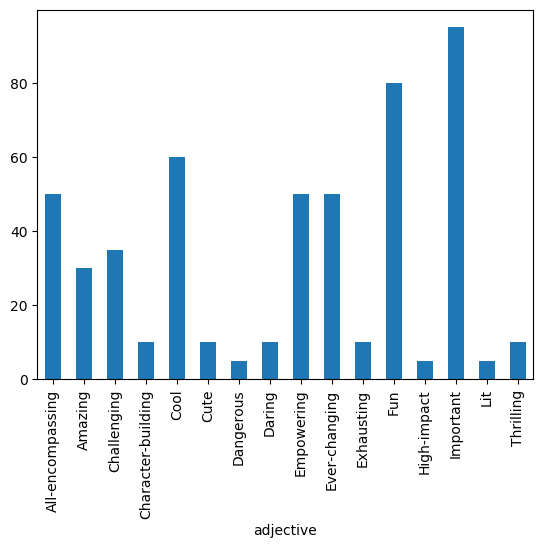
\includegraphics[width=0.7\textwidth]{adjectives.png}
\caption{Good news: Stephen spends a lot of time doing important stuff!}
\label{fig:adjectives}
\end{figure}

I know that might seem like a lot of work for ``the easy case.'' But the wild
wild world has lots of messiness, and if you want the data shown on a web page
you have to put in some elbow grease to bend it to your will. The good news is
that as far as scraping the actual \textit{page}, all we needed was one
command: \texttt{pd.read\_html()}. If the data you want from a page isn't in
\texttt{<table>}s, though, you're in for the tougher case in
Chapter~\ref{ch:screenScraping2}. Stay tuned!

   

\chapter{Screen scraping (2 of 2)}
\label{ch:screenScraping2}

\index{the easy case}
\index{screen scraping}
\index{worst of all possible worlds}

\section{The harder case: picking through the HTML tree}

Chapter~\ref{ch:screenScraping1} was the ``easy'' screen scraping case: if the
data on the web page that you want to import is in \texttt{<table>} rows, you
can (relatively) simply use Pandas' \texttt{read\_html()} function to suck it
in to Python.

For anything else, you'll have to comb through the HTML structure, figuring out
how to surgically extract what you seek. It's a major pain, but there is a
Python library by the outrageous name ``BeautifulSoup'' which makes it just a
little bit less painful. This chapter contains an overview of how to work with
it.


\section{Web Developer Tools}

\index{web developer tools}
\index{element (HTML)}

First, let me say that Firefox, Chrome, and several other browsers come
equipped with very sophisticated ``web developer tools'' that let you browse
the HTML, CSS, and rendered page, and figure out what elements got rendered via
which portions of the screen. They're very handy, and when screen scraping you
should get into the habit of using them. In Firefox, they're available via the
``Tools | Web Developer | Toggle tools...'' menu option. In Chrome, you go to
the little three vertical dots, then choose ``More Tools | Developer Tools.''


\section{Parsing with BeautifulSoup}

\index{BeautifulSoup}
\index{web crawler}
\index{URL}

As I mentioned on p.~\pageref{downloading}, it's generally recommended to
\textit{download} the web page you want to parse rather than having Python read
it for you over the network. This eliminates one more possible source of error.
(Exception: if you need a Python program to act as a \textbf{web crawler} and
read pages on demand as it discovers their URLs. More on that later.) Note that
you can still open the page in your browser even after downloading it: just go
to ``File | Open File...'' or the equivalent operation in your browser.

Once you've done this, and now have your HTML in a file called (say)
``\texttt{myfile.htm}'', you can then parse it with BeautifulSoup using:

\index{bs4@\texttt{bs4} (BeautifulSoup library)}

\begin{Verbatim}[fontsize=\small,samepage=true,frame=single,framesep=3mm]
from bs4 import BeautifulSoup
soup = BeautifulSoup(open("myfile.htm"), "html.parser")
\end{Verbatim}

\index{soup@\texttt{soup}}
\index{html.parser@\texttt{html.parser} (BeautifulSoup)}

By convention, the variable for this parsed structure is called
``\texttt{soup}''. The second argument to the \texttt{BeautifulSoup} function
tells it which \textbf{parser} we want to use to analyze the code; there are
other choices here, but stick with \texttt{"html.parser"} for now.

One possibly useful command (though limited if your web page is large) is:

\index{pretty printing@``pretty printing''}
\index{prettify@\texttt{.prettify()} (BeautifulSoup)}

\begin{Verbatim}[fontsize=\small,samepage=true,frame=single,framesep=3mm]
print(soup.prettify())
\end{Verbatim}

This ``pretty prints'' out the entire contents of the page, but in a way that
is properly indented according to the HTML's structure, rather than how it was
indented in the raw page. You may have noticed that the HTML file may or may
not be physically indented and spaced in a way reflective of the structure. The
BeautifulSoup parser is smart enough to discern the implied structure from the
tag sequence, and thus prints it how it will ``really'' be seen by a browser.

\index{top-down navigation}
\index{bottom-up navigation}

At this point, I generally take one of two approaches: either I navigate the
structure \textbf{top-down} looking for where the data I'm interested in is
situated, or I find the data by searching through the file, and use a
\textbf{bottom-up} approach to get it from there. You typically have to combine
the two approaches to get your screen-scraping dirty work done.

\subsection{The top-down approach}

\index{root node (of an HTML file)}
\index{contents@\texttt{.contents} (BeautifulSoup)}

By using ``\texttt{soup.contents}'', you get the immediate descendants of
the root node of the HTML hierarchy. Each of these could be examined for its
type, like this:

\index{type@\texttt{type()}}

\begin{Verbatim}[fontsize=\small,samepage=true,frame=single,framesep=3mm]
for child in soup.contents:
    print(type(child))
\end{Verbatim}
\vspace{-.2in}

\begin{Verbatim}[fontsize=\small,samepage=true,frame=leftline,framesep=5mm,framerule=1mm]
bs4.element.Tag
bs4.element.NavigableString
\end{Verbatim}

\index{NavigableString@\texttt{NavigableString} (BeautifulSoup)}
\index{tag (HTML)}

So our entire document is composed of an element (misleadingly named ``Tag''
here, but w/e) and a ``\texttt{NavigableString}'' which essentially just means
``string of literal text''. For elements, it's useful to print out their
``\texttt{.name}''. For strings, it's useful to print them out verbatim. Here,
we see:

\begin{Verbatim}[fontsize=\small,samepage=true,frame=single,framesep=3mm]
print(soup.contents[0].name)
print(soup.contents[1])
\end{Verbatim}
\vspace{-.2in}

\begin{Verbatim}[fontsize=\small,samepage=true,frame=leftline,framesep=5mm,framerule=1mm]
'html'
'\n'
\end{Verbatim}

\index{html@\texttt{<html>} (HTML tag)}

So the first child is the entire \texttt{html} element in all its embedded
glory, and this is followed by a single, pesky newline. Now you know.

Drilling down another level, we see:

\begin{Verbatim}[fontsize=\small,samepage=true,frame=single,framesep=3mm]
html_children = soup.contents[0]
for child in html_children:
    print(type(child))
\end{Verbatim}
\vspace{-.2in}

\begin{Verbatim}[fontsize=\small,samepage=true,frame=leftline,framesep=5mm,framerule=1mm]
bs4.element.NavigableString
bs4.element.Tag
bs4.element.NavigableString
bs4.element.Tag
bs4.element.NavigableString
\end{Verbatim}

Two tags, with three strings interleaved. Let's examine them:

\begin{Verbatim}[fontsize=\small,samepage=true,frame=single,framesep=3mm]
print(html_children.contents[0])
print(html_children.contents[1].name)
print(html_children.contents[2])
print(html_children.contents[3].name)
print(html_children.contents[4])
\end{Verbatim}
\vspace{-.2in}

\begin{Verbatim}[fontsize=\small,samepage=true,frame=leftline,framesep=5mm,framerule=1mm]
'\n'
'head'
'\n'
'body'
'\n'
\end{Verbatim}

You're starting to see a pattern: a lot of the strings are just newline
characters that split up the HTML text file and make it more readable. What we
really care about is the content under the tags. Let's dig one deeper:

\begin{Verbatim}[fontsize=\small,samepage=true,frame=single,framesep=3mm]
head_children = html_children.contents[1].contents
print(head_children[0])
print(head_children[1].name)
print(head_children[2])
print(head_children[3].name)
print(head_children[4])
\end{Verbatim}
\vspace{-.2in}

\begin{Verbatim}[fontsize=\small,samepage=true,frame=leftline,framesep=5mm,framerule=1mm]
'\n'
'title'
'\n'
'style'
'\n'
\end{Verbatim}

Okay, you get the idea. We can drill down to whatever level we want just by
following the appropriate children. To get the title of the page, we could do:

\index{title@\texttt{<title>} (HTML tag)}

\begin{Verbatim}[fontsize=\small,samepage=true,frame=single,framesep=3mm]
print(head_children[1].contents[0])
\end{Verbatim}
\vspace{-.2in}

\begin{Verbatim}[fontsize=\small,samepage=true,frame=leftline,framesep=5mm,framerule=1mm]
'All About Stephen'
\end{Verbatim}

\index{title@\texttt{<title>} (HTML tag)}
\index{head@\texttt{<head>} (HTML tag)}

(This is because the second element (element \#1) of the \texttt{<head>} element
is the \texttt{<title>} element, and its only child is the string
\texttt{\textquotesingle All About Stephen\textquotesingle}.)

Sometimes a quicker method to find your way through the forest is to use this
syntax\footnote{That thing in the boxies -- ``\texttt{[ x.name for x in
body\_children ]}'' -- is called a ``\textbf{list comprehension},'' by the way,
and is an advanced Python technique that is sometimes very useful.} at the
interactive console:

\index{list!comprehension}

\begin{Verbatim}[fontsize=\small,samepage=true,frame=single,framesep=3mm]
print([ x.name for x in body_children ])
\end{Verbatim}
\vspace{-.2in}

\begin{Verbatim}[fontsize=\small,samepage=true,frame=leftline,framesep=5mm,framerule=1mm]
[None, 'h1', None, 'p', None, 'p', None, 'h2', None, 'table', None]
\end{Verbatim}

\index{p@\texttt{<p>} (HTML tag)}

You can better see at a glance what's what. Now that we know the first
``\texttt{p}'' (paragraph) is element \#3 of the body, we could find that
hyperlink via:

\begin{Verbatim}[fontsize=\small,samepage=true,frame=single,framesep=3mm]
print([ x.name for x in list(body_children)[3] ])
\end{Verbatim}
\vspace{-.2in}

\begin{Verbatim}[fontsize=\small,samepage=true,frame=leftline,framesep=5mm,framerule=1mm]
[ None, 'a', None, 'b', None, 'u', None]
\end{Verbatim}

and grab it via:

\begin{Verbatim}[fontsize=\small,samepage=true,frame=single,framesep=3mm]
dat_hyperlink =  list(list(body_children)[3])[1]
\end{Verbatim}

\index{dictionary}
\index{attribute!of an HTML element}
\label{dictSyntax}

BeautifulSoup lets you access the attributes of an HTML element by treating
the element as a dictionary. Pretty cool. We can snag the actual link, then,
with:

\begin{Verbatim}[fontsize=\small,samepage=true,frame=single,framesep=3mm]
print(dat_hyperlink['href'])
\end{Verbatim}
\vspace{-.2in}

\begin{Verbatim}[fontsize=\small,samepage=true,frame=leftline,framesep=5mm,framerule=1mm]
'http://buildings.umwblogs.org/james-farmer-hall/'
\end{Verbatim}

\subsection{The bottom-up approach}

Sometimes, when you try to dive from the top of the document all the way to
what you want, you can find yourself in a tangled mess. In these cases it's
easier to search for the data you want using BeautifulSoup's search facilities.

Let's illustrate this by creating a simple \texttt{DataFrame} that contains
each role and its percentage allocation of Stephen's time. We want \texttt{df}
to look something like this:

\begin{Verbatim}[fontsize=\small,samepage=true,frame=leftline,framesep=5mm,framerule=1mm]
                role  perc
0  College professor  50.0
1                Dad  30.0
           . . .
\end{Verbatim}

To find our way through the forest, we search through the HTML with developer
tools, locating one of the pieces of data we know is there -- for instance, the
number \texttt{50}, which we can see on the page is one of the percentages.
When we click on this (or just search for it in a text file), we find ourselves
in the middle of the HTML content in Figure~\ref{fig:bottomUpSearch}.

\begin{figure}[ht]
\centering
\begin{Verbatim}[fontsize=\footnotesize,samepage=true,frame=lines]
...
<table border=2 cellpadding=15>
<tr><td class="pic"><img src="a.jpg"></td>
    <td class="role">College professor</td>
    <td class="description">
    Stephen teaches computer science and data science to willing undergraduates,
    shaping them into the heroes of tomorrow.
    </td>
    <td>
    <ul>
    <li>Super rewarding</li>
    <li>Exciting</li>
    <li>Ever-changing</li>
    <li>Fun</li>
    </ul>
    </td>
    <td>
    <b>50%</b> of total time
    </td>
</tr>
...
\end{Verbatim}
\caption{Using a bottom-up approach -- locating the text ``\texttt{50}'' in the
HTML file (stare towards the bottom of that HTML text) and getting one's
bearings regarding where it is in relation to other elements.}
\label{fig:bottomUpSearch}
\end{figure}
\normalsize

\index{td@\texttt{<td>} (HTML tag)}
\index{b@\texttt{<b>} (HTML tag)}
\index{class@\texttt{class} (HTML/CSS attribute)}

Looks like the role name we want is the text under a \texttt{td} element whose
class\footnote{In HTML, a ``\textbf{class}'' is an attribute used to classify
certain elements to be picked up by CSS formatting instructions. If this were a
Web development textbook, it would talk about when and how to use
``\texttt{class}''. But for our purposes, it's just one of many handy things we
might hook on to in order to find our data in the morass.} is
``\texttt{role}''. And it looks like the percentage we want is (*groan*) in a
boldface (\texttt{b}) tag, underneath the last \texttt{td} tag of the row,
which has no \texttt{class}.

\index{find\_all@\texttt{.find\_all()} (BeautifulSoup)}

BeautifulSoup's \texttt{.find\_all()} method makes this slightly less of a
headache. To quickly grab all the \texttt{tr} elements in the document, we can
do this:

\begin{Verbatim}[fontsize=\small,samepage=true,frame=single,framesep=3mm]
trs = list(soup.find_all("tr"))
\end{Verbatim}

\index{td@\texttt{<td>} (HTML tag)}

The variable \texttt{trs} is now a list of \textit{elements} (BeautifulSoup
``\texttt{Tag}'' objects) each of which we can examine for (say) \texttt{td}
children with a \texttt{role} \texttt{class} attribute. And you can call
\texttt{.find\_all()} on \textit{any} tag (to search from that point in the
hierarchy down), not just on the top-level \texttt{soup} element. So:

\index{in@\texttt{in}}
\index{array@\texttt{array()} (NumPy)}
\index{dtype@\texttt{dtype}}

\begin{Verbatim}[fontsize=\small,samepage=true,frame=single,framesep=3mm]
roles = np.array([], dtype=object)
trs = soup.find_all("tr")
for tr in trs:
    tds = tr.find_all("td")
    for td in tds:
        if "class" in td.attrs and "role" in td["class"]:
            ...
\end{Verbatim}

\index{list}
\index{dictionary}
\index{key-value pair}
\index{attribute!of an HTML element}
\index{attrs@\texttt{.attrs} (BeautifulSoup)}

The ``\texttt{.attrs}'' syntax gives us a \textit{dictionary} of key-value
pairs which represent the attributes of an element. So by saying
``\texttt{"class" in td.attrs}'' we're first checking whether there is a
\texttt{class} attribute in the current \texttt{td} element at \textit{all}
before then attempting to get its value using the dictionary syntax mentioned
on p.~\pageref{dictSyntax}.

\label{classIsAttribute}

Btw, one slight surprise in the above \texttt{if} statement might be that we're
checking whether \texttt{"role"} is \textit{\texttt{in}} \texttt{td["class"]}
instead of simply being \texttt{==} to \texttt{td["class"]}. That's because in
HTML, the \texttt{class} attribute of an tag can have \textit{multiple}
(space-separated) values, not just one, and so \texttt{td["class"]} is actually
a \textit{list}, not a single string.

\index{get\_text@\texttt{.get\_text()} (BeautifulSoup)}

Okay, now when we reach the body of that \texttt{if} statement, we have
successfully found one of the desired \texttt{td} attributes. How do we then
get the text under it? Just call \texttt{.get\_text()} on it, and then append
it to the list. This creates our desired list of roles that we can stick in our
\texttt{DataFrame}.

\begin{Verbatim}[fontsize=\small,samepage=true,frame=single,framesep=3mm]
            ...
            roles.append(td.get_text())
\end{Verbatim}

To get the percentages, we just need a slightly different approach: first,
we're going to assume the percentage is in the \textit{last} \texttt{td} tag,
and second, we need to go inside that to retrieve the percentage from the
embedded boldface tag. Adding this to our \texttt{for} loop almost gets us
there:

\begin{Verbatim}[fontsize=\small,samepage=true,frame=single,framesep=3mm]
percs = []
...
    the_bold = tds[-1].find("b")
    percs.append(the_bold.get_text())
\end{Verbatim}

although we'd like to also strip that percentage sign off and convert it to an
actual numeric value, so we'll do this instead:

\begin{Verbatim}[fontsize=\small,samepage=true,frame=single,framesep=3mm]
percs = []
...
    the_bold = tds[-1].find("b")
    percs.append(float(the_bold.get_text()[:-1]))
\end{Verbatim}

\index{find@\texttt{.find()} (BeautifulSoup)}
\index{find\_all@\texttt{.find\_all()} (BeautifulSoup)}

and now we can create our DataFrame with both columns. (Note that
``\texttt{.find()}'' does the same thing as ``\texttt{.find\_all()}'' except
that it only grabs the first matching element rather than all of them.) The
complete code is shown in Figure~\ref{fig:getRolesComplete}.

\begin{figure}[ht]
\begin{Verbatim}[fontsize=\small,samepage=true,frame=single,framesep=3mm]
roles = []
percs = []

trs = soup.find_all("tr")
for tr in trs:
    tds = tr.find_all("td")
    for td in tds:
        if 'class' in td.attrs and 'role' in td['class']:
            roles.append(td.get_text())
    the_bold = tds[-1].find("b")
    percs.append(float(the_bold.get_text()[:-1]))

df = pd.DataFrame({'role':roles, 'perc':percs})[['role','perc']]
\end{Verbatim}
\caption{The complete code example to screen scrape the roles and percentages
from the web page in Figure~\ref{fig:allAboutStephen}
(p.~\pageref{fig:allAboutStephen}).}
\label{fig:getRolesComplete}
\end{figure}

\subsection{Other BeautifulSoup features}

The BeautifulSoup library has a myriad of alternatives for navigating and
searching the tree. Here are a few.

\subsubsection{Searching by id or class}

\index{find@\texttt{.find()} (BeautifulSoup)}
\index{find\_all@\texttt{.find\_all()} (BeautifulSoup)}
\index{id@\texttt{id} (BeautifulSoup)}
\index{class\_@\texttt{class\_} (BeautifulSoup)}

\texttt{.find()} and \texttt{.find\_all()} each have optional \texttt{id} and
\texttt{class\_} (note the trailing underscore!) parameters that can be used
to restrict a search to only elements with matching attributes.

\begin{Verbatim}[fontsize=\small,samepage=true,frame=single,framesep=3mm]
soup.find_all("td", class_="pic")
\end{Verbatim}

\subsubsection{Using the Python ``dot'' syntax}

If we know the names of the tags, we can navigate a structure by using a
Pandas-like ``dot'' syntax. Check it out:

\begin{Verbatim}[fontsize=\small,samepage=true,frame=single,framesep=3mm]
print(soup.head.title)
print(soup.head.name)
print(soup.head.title.string)
print(soup.body.table.td.img['src'])
\end{Verbatim}
\vspace{-.2in}

\begin{Verbatim}[fontsize=\small,samepage=true,frame=leftline,framesep=5mm,framerule=1mm]
<title>All About Stephen</title>
title
'All About Stephen'
'a.jpg'
\end{Verbatim}


\subsubsection{Accessing all attributes}

\index{tag (HTML)}
\index{attrs@\texttt{.attrs} (BeautifulSoup)}
\index{dictionary}

As we've seen, in addition to treating an element (``\texttt{Tag}'') as a
dictionary to retrieve its element values, you can also use the
``\texttt{.attrs}'' syntax to get the dictionary directly:

\begin{Verbatim}[fontsize=\small,samepage=true,frame=single,framesep=3mm]
print(soup.body.find("a").attrs)
print(soup.body.find("td").attrs)
\end{Verbatim}
\vspace{-.2in}

\begin{Verbatim}[fontsize=\small,samepage=true,frame=leftline,framesep=5mm,framerule=1mm]
{'href': 'http://buildings.umwblogs.org/james-farmer-hall/'}
{'class': ['pic']}
\end{Verbatim}

(As noted on p.~\pageref{classIsAttribute}, see how the value of the
``\texttt{class}'' attribute is a list here.)

\subsubsection{Getting just text with \texttt{.get\_text()}}

\index{get\_text@\texttt{.get\_text()} (BeautifulSoup)}

The aforementioned \texttt{.get\_text()} method is actually a bit more
powerful than just extracting the contents of a single plain text element
underneath an element. It can also be used to get \textit{all the text} from
that point down in the hierarchy, ignoring all tags. Check it out:

\begin{Verbatim}[fontsize=\small,samepage=true,frame=single,framesep=3mm]
soup.body.find("p").get_text()
\end{Verbatim}
\vspace{-.2in}

\begin{Verbatim}[fontsize=\small,samepage=true,frame=leftline,framesep=5mm,framerule=1mm]
'Deep in the bowels of Farmer Hall resides a\ncarbon-based life form known to
outsiders only as Stephen. This\nmysterious being fulfills several roles not
widely known to\nhumankind.'
\end{Verbatim}

\subsubsection{Finding more than one tag name at once}

\index{find\_all@\texttt{.find\_all()} (BeautifulSoup)}
\index{list}

You can pass a \textit{list} to \texttt{.find\_all()} to match more than one
type of tag in a search:

\begin{Verbatim}[fontsize=\small,samepage=true,frame=single,framesep=3mm]
soup.find_all(["td", "th", "p"])
\end{Verbatim}

\index{regex (regular expression)}

And if you know how to use \textbf{regular expressions} (outside the scope of
this class) you can use them as arguments to \texttt{.find\_all()} and
friends:

\begin{Verbatim}[fontsize=\small,samepage=true,frame=single,framesep=3mm]
import re
soup.find_all(re.compile("^q"))
soup.find_all(re.compile("r"))
soup.find_all(re.compile("s$"))
\end{Verbatim}

(finds all tags whose name begin with \texttt{q}, contain \texttt{r}, or end
with \texttt{s}, respectively.)

\subsubsection{CSS selectors}

\index{CSS}
\index{select@\texttt{.select()} (BeautifulSoup)}

Finally, if you're familiar with CSS selector syntax, you can do all that jazz
by calling the \texttt{.select()} method:

\begin{Verbatim}[fontsize=\small,samepage=true,frame=single,framesep=3mm]
soup.select("div#master, tr td.data")
\end{Verbatim}

   
\chapter{About probability}
\label{ch:prob}

\index{probability}

\textbf{Probability theory} is an area of mathematics that deals with
\textit{quantifying uncertainty}. We may not be sure that something is going to
happen, but we want to be precise about \textit{how} sure we are, given
everything else we may know.

\index{random value}
\index{distribution}

It turns out that probability theory is a crucial concept in Data Science.
We've already used some of it in Chapters~\ref{ch:random} and
\ref{ch:synthetic} when we generated random values from distributions. In this
chapter, we'll zoom out from programming language details and consider how to
reason about the probabilities of various values occurring and the
relationships between random variables.

\section{Terms}

\index{outcome (probability)}
\index{redheads}
\index{Girl on the Train, The@\textit{Girl on the Train, The}}
\index{Hawkins, Paula}
\index{hardback edition}

Some terms: an \textbf{outcome} is something that may (or may not) happen. This
varies widely depending on the domain: a child that's born may or may not be
male; an airline passenger may or may not have red hair; a customer may or may
not buy a particular product. ``Male,'' ``red,'' and ``\textit{The Girl on the
Train}, hardback edition'' are all outcomes in these examples.

\index{event (probability)}
\index{DVD}

An \textbf{event}, by contrast, is a \textit{set} (group) of outcomes that
we're interested in. Often we don't care so much whether or not the customer
specifically bought ``\textit{The Girl on the Train}, hardback edition'' as
whether they bought \textit{any} book by Paula Hawkins, or maybe any hardback
book, or maybe any book at all (as opposed to a DVD).

\index{sample space (probability)}
\index{redheads}
\index{bald}
\index{brunettes}
\index{blondes}
\index{omega ($\Omega$)}
\index{$\Omega$ (omega)}

Sometimes we'll use the symbol $\Omega$ (``omega'') to refer to the
\textbf{sample space}, which is simply the set of \textit{all possible
outcomes}. This will vary depending on what's under consideration; it might be
\{ male, female \} in one case and \{ red, blonde, brunette, bald, other \} in
another case.

We'll also use the notation $\overline{\phantom{xx}}$ (overbar) to mean ``any
outcome \textit{except} something.'' For instance, $\overline{\textrm{red}}$
means ``the airline passenger had a hair color \textit{other than} red.''

\section{Probability measures}

\index{probability measure}

A \textbf{probability measure} is a function that tells us intuitively how
likely an outcome is to occur. We'll use the simple notation ``P($\cdot$)'' for
this\footnote{Some authors use ``Pr()'' instead of ``P()'' for this. Same
diff.}, read as ``the probability of (something).'' The probability of any
outcome is always \textit{a number between 0 and 1}. 0 means it can never
possibly occur, 1 means it will definitely occur, and there's a continuum in
between. In our first example, we might say P(male) = .5, P(red) = .1, and
P(\textit{The Girl on the Train}, hardback edition) = .0001.

You can talk about the probability of an event too, of course, and it's simply
the sum of the outcome probabilities. P(male-or-female) = 1, P(red or blonde
or bald) = .6, P(any hardcover book) = .08. We'll say that P($\Omega$) will be
1: after all, \textit{something} has to happen, even if it's ``the customer
didn't buy anything,'' an outcome to which we'll assign a probability.

\section{``Joint'' probability}
\index{redheads}
\index{joint probability}
\index{,@, (comma) (joint probability)}
%\index{pipe@\|\ (pipe) (conditional probability)}

Very commonly, we'll be considering the likelihood that two different events
\textit{both} occur. For instance, perhaps we're interested in the probability
that an airline passenger is a red-headed female. We'll write this as P(red,
female).\footnote{You may also run across the notation
``P(red\textbf{\^{}}female),'' which means the same thing.} The comma signals
\textbf{joint probability}, which simply means that both of these
outcomes/events must occur in order for the combined event to be considered to
have occurred. If we wrote P(red, $\overline{\textrm{female}}$), it would mean
`the probability that the passenger is a red-headed \textit{non}-female.''

If you think about it, you'll realize that the joint probability cannot be
greater than either of the two individual probabilities. Adding another
condition (not female) to the first (red-headed) can't possibly
\textit{increase} the chance of it happening. Other than that, we don't know
how to compute the joint probability from the individual ones, though (yet).

Finally, note that P(A,B) is the same thing as P(B,A), guaranteed. Switching
the order of terms in a \textit{joint} probability doesn't change the answer.
(This will \textit{not} be true in the next section, so watch out!)

\section{``Conditional'' probability}

\index{conditional probability}
\index{college degree}
\index{unemployed}

Another notion we'll use a great deal is \textbf{conditional probability},
written with a ``pipe'' (vertical bar) like P(unemployed $|$\ college degree),
or P(red $|\ \overline{\textrm{female}}$). The second of these means ``if I
know for a fact that the passenger is not female, what's the probability that
they're red-headed?'' Notice this is very different than the joint probability.
With conditional probability, we're assuming that the second event
\textit{does} occur, and then asking how that revises our original prediction.
Unlike with joint probability, adding a vertical bar \textit{can} make the
answer increase.

\index{pinterest}

Consider this example: what's the probability that a random U.S. citizen has a
Pinterest account? Let's estimate that as P(pinterest) = .15. But what if we
learned that the chosen person was female? What is P(pinterest $|$ female)?
Just to shamelessly stereotype, I'm going to go out on a limb and say it's
higher; perhaps .26. On the other hand, what if we learned the person was male?
What is P(pinterest $|$ male)? I'll say it's more like .04. In both cases, we
adjusted our estimated probability in light of additional information: up in
one case, and down in the other.

\index{Bayesian reasoning}

This adjusting-our-estimates stuff is at the heart of what's called
``\textbf{Bayesian reasoning}'' (you'll see why in section~\ref{sec:bayes},
below).

\index{prior (probability)}
\index{posterior (probability)}

Two other terms that come up frequently are ``\textbf{prior probability}'' and
``\textbf{posterior probability}''. The ``\textbf{prior}'' is the probability of
an event \textit{without} applying conditioning. In the previous example .15
was the ``prior probability'' that the person was a pinterest user. When we
learned our subject was female, we revised that to the ``\textbf{posterior}''
of .26.

\index{NBA}
\index{tall}

Finally, note that P(A$|$B) is \textbf{\textit{not}} the same thing as
P(B$|$A). I gave you a heads-up about this above. In general, P(A$|$B) and
P(B$|$A) are very different numbers. Ask yourself this: if you chose a random
American, and they turned out to be pretty tall (say, taller than average),
what's the probability that they're also an NBA player? I think you'll agree
that the number here would be very small indeed: perhaps P(NBA$|$tall) would be
.00001. There just aren't that many NBA players out there, so the chances of
you randomly choosing one -- tall or not -- is miniscule. But consider the
reverse question: if your random choice just happened to be an NBA player,
what's the probability that they'd also be tall? This, by contrast, would be
far greater: I'll bet P(tall$|$NBA) is close to .95, since nearly all
professional basketball players are pretty tall.

Or continue the pinterest example. P(pinterest $|$ female) might be .26
(\textit{i.e.}, 26\% of all females are pinterest users), but P(female $|$
pinterest) might be .87 (87\% of all pinterest users are females). We'll
quantify all this in the next section.

%\section{The relationship between joint and conditional}
%
%\index{joint probability}
%\index{conditional probability}
%
%Mathematically, here's how these two concepts (joint probability and
%conditional probability) are related. If A and B are two events, then:
%
%\vspace{-.2in}
%\begin{align*}
%\boxed{P(A|B) = \frac{P(A,B)}{P(B)}}
%\end{align*}
%
%Suppose I knew that the probability of a random U.S. citizen being a
%\textit{male pinterest user} was .04. And now suppose I knew that about half
%of U.S. citizens are male. Then, I could compute:
%
%\vspace{-.2in}
%\begin{align*}
%P(\textrm{male,pinterest}) = .04 \\
%P(\textrm{male}) = .5 \\
%P(\textrm{pinterest} | \textrm{male}) &= \frac{P(\textrm{male},
%\textrm{pinterest})}{P(\textrm{pinterest})} \\
%                    &= \frac{P(\textrm{pinterest},
%\textrm{male})}{P(\textrm{pinterest})} \\
%                    &= \frac{.04}{.15} = .267 \\
%\end{align*}
%
%\section{Bayes' Rule}
%\label{sec:bayes}
%
%Knowing how joint and conditional probabilities are related, and knowing that
%P(A,B) = P(B,A), we can derive the following law:
%
%\vspace{-.2in}
%\begin{align*}
%P(A|B) = \frac{P(B|A) \cdot P(A)}{P(B)}
%\end{align*}
%
%This is called \textbf{Bayes' Rule} (sometimes \textbf{Bayes' Law} or
%\textbf{Bayes' Theorem}) after the 18th-century Presbyterian minister Thomas
%Bayes. It is one of the most influential (and controversial, actually)
%statements in statistics and even all of mathematics.
%
%\section{Independence}
%
%We need one more background concept before we attack Na\"{i}ve Bayes Classifiers,
%and that is the \textbf{independence} of events.
%
%Simply put, two events are ``independent'' if \textit{whether one of them
%occurs has no bearing on whether the other one occurs}. It does \textit{not}
%mean the events are mutually exclusive. It means that the probability of each
%one of them occurring has nothing to do with the other.
%
%It's best seen through an example. Suppose I chose a random U.S. citizen, and
%I observe two things: whether or not they're white, and whether or not they're
%female. If I asked you for your estimate of the ``prior'' for the race
%question, you'd probably come up with something like P(white) = .6. Now I ask
%you: suppose, before observing their race, that you learned your subject was
%female. Does this cause you to update your ``prior'' estimate to a more
%accurate ``posterior''?
%
%The answer is no. Whether or not someone is white is \textit{independent} of
%whether they're female. You thought P(white) was .6, and you still think
%P(white$|$female) is .6. The opposite was true in the pinterest example: your
%estimate of their pinterest status \textit{did} change when you learned about
%their gender. Therefore, those two events are \textit{not} independent.
%
%Both of the following mathematical identities are true \textit{\textbf{only
%\underline{if}}} the events $A$ and $B$ are independent:
%\vspace{-.2in}
%\begin{align*}
%P(A,B) &= P(A) \cdot P(B) \\
%P(A|B) &= P(A)
%\end{align*}
%
            

\chapter{Causality}

\index{causal relationship}
\index{observational study}
\index{controlled experiment}

I must now ask you to reach in your memory banks alllll the way back to
Chapter~10 of the \textit{previous} volume of this book series. That chapter,
entitled ``Interpreting Data,'' dealt with association vs.~causality,
confounding factors, controlled experiments vs.~observational studies, and
related topics. The key question we addressed was how to interpret a
statistical association between variables. If two variables are correlated,
then they're correlated...but how confident can we be that there's a
\textbf{causal} relationship between them -- which is what we usually care
about?

\index{causal diagram}
\index{barbecue}
\index{cancer}

\vspace{-.1in}
\begin{figure}[ht]
\begin{minipage}{6in}
\raisebox{-.5\height}{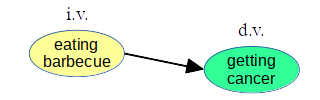
\includegraphics[width=0.45\textwidth]{causalDiagram.png}}
\raisebox{-.5\height}{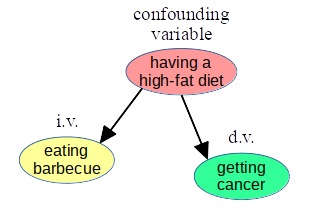
\includegraphics[width=0.45\textwidth]{causalDiagram2.png}}
\vspace{-.15in}
\caption{Causal diagrams, each expressing a hypotheses about the causality
among variables.}
\label{fig:causalDiagrams}
\end{minipage}
\end{figure}
\vspace{-.05in}

The tool we used for this analysis was the \textbf{causal diagram}, examples of
which appear in Figure~\ref{fig:causalDiagrams}. Each bubble represents one
variable. Arrows pointing from one bubble to another asserts a causal
relationship between the two: that the value of one is not merely
\textit{associated with}, but is partially \textit{responsible for}, the value
of the one pointed at. 

If you remember that particular example, there was an observational study
suggesting that eating barbecue can increase one's risk of various types
cancer. Assuming that an association between the two variables was in fact
discovered, the two sides of Figure~\ref{fig:causalDiagrams} represent
competing theories as to the reasons for that association.

The question we'll ask in this chapter is as follows: given a data set, is
there any way to actually \textit{tell} which of several competing causal
theories is true? In other words, if we have more than one hypothesis giving
alternate explanations for how the patterns in the data set arrived, can the
\textit{data itself} be used to judge between them?

And the answer is: sometimes. Let's learn when it can, and when it cannot.

\section{The bad news: identical ``skeletons''}

Before I get you too excited, let me say right at the outset that there are
times when the data fails us in our quest to nail this down. This happens when
the \textbf{skeleton}s of the two causal models are identical.

\index{skeleton (of a causal diagram)}
\index{smoking}
\index{depression}

The skeleton of a causal diagram is simply the diagram you get if you
\textit{remove the arrowheads}. Consider the two competing models in
Figure~\ref{smokingDepression}. An observational study some years ago found an
association between smoking cigarettes and experiencing clinical depression,
and made the claim that therefore one of the many detriments to smoking
(besides heart disease, lung cancer, and other things) was an emotional one.
That represents the causal model on the left side of the diagram. But some
objected and said, ``wait a minute...couldn't it instead be the case that
people who are going through depression are seeking ways to cope with it, and
that substances like nicotine could be one of those ways?'' This
depression-causes-smoking hypothesis is on the right side. 

\vspace{-.15in}
\begin{figure}[ht]
\begin{minipage}{6in}
\raisebox{-.5\height}{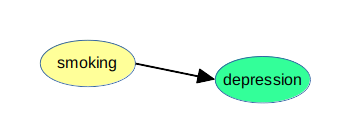
\includegraphics[width=0.45\textwidth]{smokingDepression.png}}
\raisebox{-.5\height}{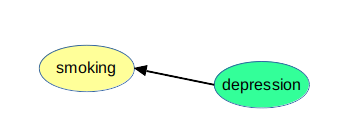
\includegraphics[width=0.45\textwidth]{depressionSmoking.png}}
\vspace{-.15in}
\caption{Does smoking cause depression...or does depression lead to smoking?}
\label{smokingDepression}
\end{minipage}
\end{figure}
\vspace{-.05in}

Unfortunately there is no way to resolve this by looking at the data alone.
This is because if you remove the (one) arrowhead, you get the same skeleton
(Figure~\ref{smokingDepressionSkeleton}). Note that ``the same skeleton'' means
merely \textit{the same bubbles are connected to the same bubbles.} It does
\textit{not} have anything to do with where those bubbles are positioned on the
page.

\vspace{-.1in}
\begin{figure}[ht]
\begin{center}
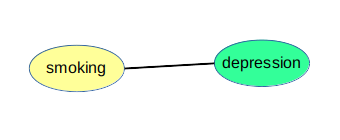
\includegraphics[width=0.8\textwidth]{smokingDepressionSkeleton.png}
\vspace{-.15in}
\caption{The bad case: both causal diagrams have the \textit{same} skeleton.}
\label{smokingDepressionSkeleton}
\end{center}
\end{figure}
\vspace{-.05in}

In this case, the only way to resolve which of the causal models is the true
one is to investigate the phenomenon on the ground. We have to study the
mechanisms -- physical and societal -- by means of which each of them might
plausibly cause the other. Medical researchers could explore the effects of
nicotine on the human brain, and determine whether there is a mechanism by
which serotonin is reduced. Social psychologists could conduct surveys and
focus groups and learn how often cigarettes are sought by victims of depression
and why. But the data itself will not give a verdict.


\section{The good news: different ``skeletons''}

Often, though, the situation isn't that dire. Consider the controversy raised
in one of my recent freshman seminars. The class was discussing the invention
of chopsticks, and the impact that may have had on eastern culture as well as
culinary techniques. One student made a different kind of claim. He said,
``this is why so many of the great video game players in the world are from
Asian countries! When kids from those regions grow up using chopsticks, it
demands more attention to fine motor skills than using a fork would. And when
they develop this terrific finger-eye coordination at a young age, it leads to
greater expertise with a controller or keyboard. Thus they are better equipped
to compete in high-level gaming.''

Perhaps. But as I listened to this student, I couldn't help remembering what my
own boys told me: that many of the Asian countries place a higher cultural
value on video games than we do in the western world. Apparently,
high-achieving video game players are afforded the same fame and fortune in
South Korea or Japan that our NFL and NBA players are in the U.S. They are
awarded lucrative contracts, perform paid testimonial advertising, give
autographs to cheering throngs, and so forth. It stands to reason, then, that a
culture which rewards excellent video game play would produce excellent video
gamers \textit{regardless} of whether those players used forks or chopsticks.

\vspace{-.15in}
\begin{figure}[ht]
\begin{center}
\raisebox{-.5\height}{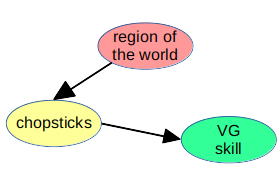
\includegraphics[width=0.4\textwidth]{chopsticksVG.png}}
\quad
\raisebox{-.5\height}{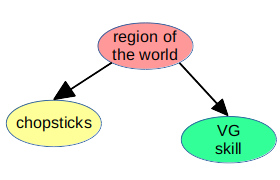
\includegraphics[width=0.4\textwidth]{regionVG.png}}
\vspace{-.05in}
\caption{Two competing causal models about why many great video game
players are from Asian countries.}
\label{chopsticksVG}
\end{center}
\end{figure}
\vspace{-.05in}

These two competing hypotheses are illustrated in Figure~\ref{chopsticksVG}.
On the left is my student's model: the region of the world you're in (Asian or
non-Asian) influences whether or not you primarily use chopsticks at your
meals. With this much, I agree. But he then further claims that the use of
chopsticks \textit{causally influences} how good a video game player you are.

The right side of the diagram shows my own mental model: the region of the
world you're in causally influences both chopstick usage \textit{and} video
game prowess. In my model, \textsf{chopsticks} and \textsf{VG skill} are
\textit{associated}, but not \textit{causally} associated.

Now before we go on, consider the following exercise. Without even knowing the
technical detail that comes next, can you figure out how to confirm or refute
my student's (left-hand) causal model? What could you do with the data?

\index{conditional probability}
\index{conditioning@``conditioning on'' (probability)}
\index{confounding factor}

The solution is intuitive to many, but not to all. Simply put, you
\textbf{condition on} the \text{region of the world} variable. This means you
split the data into two groups: those from Asian countries and those from
non-Asians countries. Think about it: if you \textit{considered only Asians},
and discovered that chopstick-using Asians are better video gamers than
non-chopstick-using Asians, then that would lend credence to the hypothesis
that one causes the other. (And the same goes for considering only non-Asians.)
But if you looked only at Asians (or only at non-Asians) and found that
chopsticks and video game skill are \textit{un}correlated, then that pretty
much refutes the hypothesis. Everything in the coming sections is an
elaboration of that principle.

\subsection{Comparing the skeletons}

\index{skeleton (of a causal diagram)}
The reason this example turns out to be one of the ``good news`` cases is that
the skeletons of the causal diagrams are different. Check out
Figure~\ref{chopsticksVGskeleton}. At first glance, you might assume that they
are the same, just as in the smoking/depression example. After all, they're
both chains-of-three nodes. But they're \textit{not} the same. In one,
\textsf{chopsticks} is the bubble with connections to the other two, and in the
other it's \textsf{region of the world}. Just because they're the same shape
doesn't mean they're the same skeleton: the same bubbles have to be connected
to the same bubbles.

\vspace{-.15in}
\begin{figure}[ht]
\begin{center}
\raisebox{-.5\height}{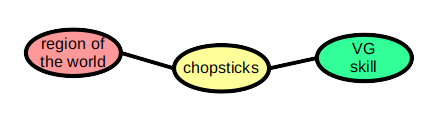
\includegraphics[width=0.45\textwidth]{chopsticksVGskeleton.png}}
\quad
\raisebox{-.5\height}{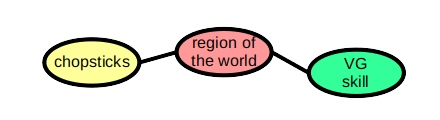
\includegraphics[width=0.45\textwidth]{regionVGskeleton.png}}
\vspace{-.05in}
\caption{The good case: the causal diagrams have \textit{different}
skeletons.}
\label{chopsticksVGskeleton}
\end{center}
\end{figure}
\vspace{-.05in}

And since the skeletons are different, the data can distinguish between the
two, and tell us which causal model (or neither) is likely to be correct.

\subsection{Reasoning about independence}

\index{independence (probability)}

The reason we can use the data to render a verdict on our competing causal
diagrams is that they embody different \textit{independence assumptions}.

Look carefully at the left side of Figure~\ref{chopsticksVG} on
p.~\pageref{chopsticksVG}. If that causal model were true, then
\textsf{chopsticks} and \textsf{VG skill} would not be absolutely independent.
Nor would \textsf{region of the world} and \textsf{VG skill}: after all, if
you're from an Asian country, you're more likely to use chopsticks, and if you
use chopsticks, you're more likely to be good at video games, so of course
the \textsf{region of the world} and \textsf{VG skill} variables are
correlated.

\index{conditional independence}
\index{conditional probability}

However, in that left-hand diagram, \textsf{region of the world} and \textsf{VG
skill} will be \textit{\underline{conditionally} independent given
\textsf{chopsticks}}. In symbols:

\vspace{-.1in}
\begin{samepage}
\begin{align*}
P(\textrm{VG}\ |\ \textrm{region}) \neq P(\textrm{VG})
\end{align*}
\begin{center}
\textit{but}
\end{center}
\vspace{-.1in}
\begin{align*}
P(\textrm{VG}\ |\ \textrm{region},\ \textrm{chopsticks}) =
P(\textrm{VG}\ |\ \textrm{chopsticks})
\end{align*}
\end{samepage}

Why is this? Because in the left-hand diagram, the only reason that knowing
a person's \textsf{region} was of any use to predicting their \textsf{VG skill}
was because it influenced how likely it was that they used \textsf{chopsticks}.
If you actually \textit{have} the information about \textsf{chopsticks}
directly, well then you can toss \textsf{region} out the window. It's
irrelevant at that point.

The right-hand side of Figure~\ref{chopsticksVG} is much different. Its
independence assumptions are that \textsf{VG skill} and
\textit{\textsf{chopsticks}} are conditionally independent given
\textit{\textsf{region}}. Namely:

\vspace{-.1in}
\begin{samepage}
\begin{align*}
P(\textrm{VG}\ |\ \textrm{region}) \neq P(\textrm{VG}) \quad \textrm{(again)}
\end{align*}
\begin{center}
\textit{but}
\end{center}
\vspace{-.1in}
\begin{align*}
P(\textrm{VG}\ |\ \textrm{chopsticks},\ \textrm{region}) =
P(\textrm{VG}\ |\ \textrm{region})
\end{align*}
\end{samepage}
\vspace{-.1in}

This is the flip side of the former case: now, although \textsf{chopsticks} can
tell you something useful about \textsf{VG skill} in a pinch, the primary
influencer of gaming skill is not \textsf{chopsticks}, but
\textit{\textsf{region}}. Once you tell me what region of the world somebody is
from, I have much better information about their possible video game use, and
knowing whether they use chopsticks is no longer of interest to me.

\bigskip

To sum up: both models agree that

\vspace{-.1in}
\begin{align*}
P(\textrm{VG}\ |\ \textrm{region}) \neq P(\textrm{VG}).
\end{align*}
\vspace{-.1in}

But the left one (my student's hypothesis) asserts:

\vspace{-.1in}
\begin{align*}
P(\textrm{VG}\ |\ \textrm{region},\ \textrm{chopsticks}) &=
P(\textrm{VG}\ |\ \textrm{chopsticks})\\
P(\textrm{VG}\ |\ \textrm{chopsticks},\ \textrm{region}) &\neq
P(\textrm{VG}\ |\ \textrm{region}),
\end{align*}
\vspace{-.1in}

while the right one (my own hypothesis) asserts:

\vspace{-.1in}
\begin{align*}
P(\textrm{VG}\ |\ \textrm{region},\ \textrm{chopsticks}) &\neq
P(\textrm{VG}\ |\ \textrm{chopsticks})\\
P(\textrm{VG}\ |\ \textrm{chopsticks},\ \textrm{region}) &=
P(\textrm{VG}\ |\ \textrm{region}).
\end{align*}

(Note carefully the ``='' vs.~``$\neq$'' signs in those equations, because
they're the only difference!)

Armed with this insight, we realize that judging between our alternate causal
models boils down to analyzing the data to see which conditional independence
assumptions actually hold. Let's see how to do that.

\section{Testing the data for conditional independence}

      

\chapter[Na\"{i}ve Bayes (1 of 3)]
{\LARGE ML classifiers: Na\"{i}ve Bayes (1 of 3)}
\label{ch:naiveBayes1}

\index{machine learning (ML)}

For some folks, the coolest and most exciting parts of Data Science are the
\textbf{machine learning (ML)} algorithms. These are the under-the-hood
techniques for doing prediction and analytics. We'll look at a few of them
briefly in this class, and you'll delve into them more fully in later courses.

\index{classifier}
\index{label}
\index{class (ML classifiers)}

Recall that a \textbf{classifier} is an algorithm/program to predict which of
several \textbf{labels} (or \textbf{classes}) to assign to a data point.
Perhaps we're trying to predict what political party someone is affiliated
with, and our labels are ``Democrat,'' ``Republican,'' and ``Green.'' Perhaps
we're trying to predict whether someone will default on a loan, and the labels
are ``safe'' and ``high-risk.''

\index{labeled example}
\index{unlabeled example}
\index{example, labeled vs.~unlabeled}
\index{training data}

There are many different algorithms for classification, but they all use a set
of \textbf{labeled examples} as ``\textbf{training data}.'' The idea is that by
scrutinizing a bunch of examples for which we \textit{know} the label, we can
intelligently figure out what label to assign to new, \textbf{unlabeled
examples}.

\index{feature}
\index{target}

The attributes of our training data (and new data) that we'll use for
prediction are sometimes called \textbf{features}. If our training data is in
a DataFrame, the features are essentially all the relevant columns except for
one, which is the \textbf{target}. Our goal, given a new data point that has
values for all the features, is to label its target with the label it's most
likely to have, assuming the training data are representative examples. 

\index{performance (of a classifier)}
\index{test data}

A classifier's \textbf{performance} can be measured in several ways, but the
most straightforward is to score how many unlabeled examples it gives the
correct label to. This of course begs the question: if the example is
\textit{un}labeled, how can we know whether or not the classifier's label was
correct? What we have to do in practice is set aside some of our (precious)
labeled data as a set of \textbf{test data}. We sort of pretend we don't know
the answers for the test data, feed them to the algorithm which has been
trained on the \textit{training} points, and then score how well it did.

\index{Na\"{i}ve Bayes classifier}
\index{baseline}

One of the simplest (and quickest) classifiers around is called the
\textbf{Na\"{i}ve Bayes classifier}, for reasons which will become apparent. In
some ways, it's the rock-bottom, no-frills default algorithm for
classification. One reason it's important is that it's simple and actually
works surprisingly (even embarrassingly) well in many cases. Another reason is
that even when it doesn't turn out to have the best performance, it's still a
\textbf{baseline} which other algorithms' performance can be compared to. A
researcher might report: ``our whiz-bang algorithm X got 89.4\% of examples
correct on this test set, compared with 83.7\% for straightforward Na\"{i}ve
Bayes.''

\section{The Na\"{i}ve Bayes algorithm}

\index{spycam}
\index{security camera}

Suppose we're designing a security system for a Galactic Cruiser. One thing we
need to do is identify possible evildoers on our security cameras. Given what
we can observe about them, can we tell good guys from bad guys?

\index{training data}
\index{security\_cam@\texttt{security\_cam.csv}}
\label{jediTraining}

\begin{Verbatim}[fontsize=\small,samepage=true,frame=leftline,framesep=5mm,framerule=1mm]
     face  height  demeanor lightsaber  type
    clean   short  menacing      green  Sith
    beard  medium      calm      green  Jedi
    clean    tall  menacing        red  Sith
    beard  medium      calm       blue  Jedi
    beard  medium      calm       blue  Jedi
    clean  medium      calm       blue  Sith
    clean    tall  menacing        red  Jedi
    clean  medium  menacing        red  Sith
    clean   short      calm       blue  Jedi
                    . . .
\end{Verbatim}

\index{feature}
\index{label}
\index{target}
\index{Jedi}
\index{Sith}

The training data above, in a \texttt{DataFrame} called ``\texttt{t}'' (for
``training''), has four features: whether the \texttt{face} of the person in
question has a \texttt{beard} or is \texttt{clean}-shaven, what their
\texttt{height} is (clustered in three broad ranges), whether their
\texttt{demeanor} is \texttt{menacing} or \texttt{calm}, and what color
\texttt{lightsaber} they wield. The final column is our label: this person is
known to be a \texttt{Jedi} (good guy) or a \texttt{Sith} (bad guy).

A test point that we might want to evaluate looks like this:
\begin{Verbatim}[fontsize=\small,samepage=true,frame=leftline,framesep=5mm,framerule=1mm]
     face  height  demeanor lightsaber  type
    beard   short  menacing        red   ?? 
\end{Verbatim}


In other words, a short, menacing, bearded person with a red lightsaber has
just showed up on security camera \#305. Should we sound the alarm? That, of
course, depends upon their (as yet unknown) \texttt{type}. We want to predict
this based on our past examples.

\index{conditional probability}
\bigskip

The \textbf{Na\"{i}ve Bayes} classification algorithm applies conditional
probability to this question. Really, what we're asking is: ``which of the
following two quantities is greater:

\begin{compactenum}
\item P(Jedi\ $|$\ beard,short,menacing,red),  or
\item P(Sith\ $|$\ beard,short,menacing,red)?''
\end{compactenum}
 
Note that we're combining joint and conditional probabilities here. Given that
we have the \textit{joint} event ``bearded, short, menacing, and red,'' what's
the \textit{conditional} probability of them being a Jedi (or Sith)? If we
estimate the first as .8 and the second as .2, for instance, we won't sound the
alarm.

\section{Using Bayes' rule}

\index{Bayes' Rule (probability)}

With Bayes' rule, we can rewrite these as:

\footnotesize
\begin{center}
(1) Estimated Jedi probability:

\boxed{\textrm{P(Jedi | beard,sh,menace,red)} =
\frac{\textrm{P(beard,sh,menace,red | Jedi)} \cdot \textrm{P(Jedi)}}{\textrm{P(beard,sh,menace,red)}}}
\end{center}
\normalsize

and
\footnotesize
\begin{center}
(2) Estimated Sith probability:

\boxed{\textrm{P(Sith | beard,short,menace,red)} =
\frac{\textrm{P(beard,short,menace,red | Sith)} \cdot \textrm{P(Sith)}}{\textrm{P(beard,short,menace,red)}}}
\end{center}
\normalsize

Note that the two equations are identical except for the words ``Jedi'' and
``Sith,'' which are interchanged. Let's focus on equation (1) first.

Bayes' Rule has allowed us to turn things on their head. In essence, instead of
asking ``if they have these physical features, would they likely be a Jedi?''
we're asking ``if they're a Jedi, would they be likely to have these physical
features?'' 

\index{prior (probability)}

\index{numerator}

The right-hand side of equation (1) has three parts: two in the numerator, and
one in the denominator. Ignore the denominator for a moment. The second part of
the numerator, P(Jedi), is our \textbf{prior} probability. That's easy to
estimate from the training data: we just count up what percentage of our
samples are Jedi overall.

The first half of the numerator needs more work. It reads:

\vspace{-.2in}
\begin{align*}
P(\textrm{beard},\textrm{short},\textrm{menacing},\textrm{red}\ |\ \textrm{Jedi}) 
\end{align*}

\index{independence (probability)}

Now \textbf{\textit{\underline{if}}} \ it just so happened that those four
features were \textit{independent} of one another, this would actually be
super easy to compute. We could just do this:

\vspace{-.2in}
\begin{align*}
P(\textrm{beard} \ |\ \textrm{Jedi}) \cdot
P(\textrm{short} \ |\ \textrm{Jedi}) \cdot
P(\textrm{menacing} \ |\ \textrm{Jedi}) \cdot
P(\textrm{red} \ |\ \textrm{Jedi})
\end{align*}

Under this outrageous assumption, we've split the expression into \textit{each
feature individually.} This is called \textbf{the Na\"{i}ve Bayes assumption}.
Of course it's probably \textit{not} true that beardedness, height, demeanor,
and lightsaber color are all independent of each other; for one thing, if some
or all of these features are indicative of Jedi-ness (which we hope), then they
certainly \textit{will} vary together! But the Na\"{i}ve Bayes classifier says
``aw heck, let's just throw caution to the wind and see how things work out.''

All these components are now trivially obtainable from the training data. For
example, what's a good estimate of P(beard $|$ Jedi)? Simple: look at
\textit{only the Jedi} in the training data, and count up how many
``\texttt{beard}s'' and ``\texttt{clean}s'' there are. The fraction that are
\texttt{beard}s is our estimate of P(beard $|$ Jedi).\footnote{If you have
trouble seeing this, go back to the definition of conditional probability on
p.~\pageref{condProbDef}. We're really calculating
$\dfrac{P(\textrm{beard},\textrm{Jedi})}{P(\textrm{Jedi})}$ here, which is
``the number of bearded Jedi divided by the number of total Jedi.''}

To make it concrete, in our training data on p.~\pageref{jediTraining}, there
are a total of six Jedi (count them!), of whom four have beards (count them!).
Therefore, our estimate for P(beard $|$ Jedi) is $\frac{4}{6} = \frac{2}{3}$.
In other words, based on this training data, we guesstimate that if you're a
Jedi, it's about 67\% likely that you're bearded.

\section{A numerical example}

\label{jediNumerical}
\index{numerator}

Let's work out the numerical answer (numerator only) for the training data
listed earlier. First, considering \textit{only} the five \texttt{Jedi} rows
gives us our Jedi numerator:

\smallskip
\footnotesize
% Whew! See array package documentation.
\hspace{-.2in}
\begin{tabular}{>{$}c<{$}@{$\ \cdot\ $}>{$}c<{$}@{$\ \cdot\ $}>{$}c<{$}@{$\
\cdot\ $}>{$}c<{$}@{$\ \cdot\ $}>{$}c<{$}>{$}l<{$}}
P(\textrm{beard}|\textrm{Jedi}) &
P(\textrm{short}|\textrm{Jedi}) &
P(\textrm{menace}|\textrm{Jedi}) &
P(\textrm{red}|\textrm{Jedi}) & P(\textrm{Jedi}) &= \\
\frac{4}{6} & \frac{1}{6} & \frac{2}{6} & \frac{1}{6} &
\frac{6}{11} &= .0034
\end{tabular}
\normalsize

\bigskip
Now let's do the same thing for the five \texttt{Sith} rows to get the Sith
numerator:

\footnotesize
\smallskip
\hspace{-.2in}
\begin{tabular}{>{$}c<{$}@{$\ \cdot\ $}>{$}c<{$}@{$\ \cdot\ $}>{$}c<{$}@{$\
\cdot\ $}>{$}c<{$}@{$\ \cdot\ $}>{$}c<{$}>{$}l<{$}}
P(\textrm{beard}|\textrm{Sith}) &
P(\textrm{short}|\textrm{Sith}) &
P(\textrm{menace}|\textrm{Sith}) &
P(\textrm{red}|\textrm{Sith}) & P(\textrm{Sith}) &= \\
\frac{1}{5} & \frac{1}{5} & \frac{4}{5} & \frac{2}{5} &
\frac{5}{11} &= .0058\\
\end{tabular}
\normalsize

\bigskip
Look very very carefully at the training data on p.~\pageref{jediTraining} and
confirm that you agree with the above numbers. Using a pencil to write marks
on the training data often helps you to keep everything straight.

\subsection{Throw away the denominator}

\index{denominator}
\index{throwing away the denominator}

Okay, those are the two numerators. To get true probabilities, we have to
divide by the denominators, of course. But the nice thing is: \textit{the
denominators are the \underline{same} in the two cases!} For both expressions,
we would need to divide by P(\textrm{beard}, \textrm{short}, \textrm{menacing},
\textrm{red}) (in words, ``what's the probability that any random person would
be a bearded, short, menacing person with a red lightsaber?'') This of course
has the same value even if we compute it twice. For this reason, we
\textit{throw away the denominator} since in the end all we really care about
is ``which is higher, P(Jedi $|$ \textsl{stuff}) or P(Sith $|$
\textsl{stuff})?''

In this case, P(Sith $|$ \textsl{stuff}) is the higher of the two quantities
(.0058 vs.~.0034) and so we boldly predict: ``this person looks like a Sith!
Sound the alarm.''

\bigskip
All that counting and dividing, of course, is a pain. So we'll get Python to
automate it for us. That's the subject of the next chapter.
             
% ADD SKLEARN STUFF (SEE JEDISCIKIT.PY)
% INCLUDING ONE-HOT ENCODING


\chapter[ML classifiers: Na\"{i}ve Bayes (2 of 3)]
{\huge ML classifiers: Na\"{i}ve Bayes (2 of 3)}
\label{ch:naiveBayes2}

How can we automate the calculations of the previous chapter in Python? Let's
assume that our data is in a Pandas \texttt{DataFrame} called ``\texttt{t}''
(for ``training'') as it was in the last chapter (p.~\pageref{jediTraining}).
Now imagine writing this function:

\index{predict@\texttt{predict()} (Jedi/Sith)}

\begin{Verbatim}[fontsize=\small,samepage=true,frame=single,framesep=3mm]
def predict(face, height, demeanor, lightsaber):
    ...
\end{Verbatim}

\index{Jedi}
\index{Sith}

This function takes as input a new (unlabeled) data point and returns a
prediction for it: either the word ``\texttt{Jedi}'' or the word
``\texttt{Sith}.''

\index{training data}

We'll do most of the work outside the function, actually. We'll read in the
file and then pre-compute all the probabilities that we'll need for our
calculations. This is effectively the training stage: we're ``training'' our
classifier function on the data.

If you think it through, the calculations from Chapter~\ref{ch:naiveBayes1}
imply the need for the following probabilities:

\index{prior (probability)}
\index{conditional probability}

\begin{compactitem}
\item $P(label)$ for every one of the target labels (these are the ``priors'')
\item $P(value\ |\ label)$ for every value in a column and every target label
(the conditionals)
\end{compactitem}

In our case, this amounts to:

\begin{compactitem}
\item Priors:
    \begin{compactitem}
    \item $P(\textrm{Jedi})$
    \item $P(\textrm{Sith})$
    \end{compactitem}

\item Conditionals:
    \begin{compactitem}
    \item $P(\textrm{clean}\ |\ \textrm{Jedi})$ and
$P(\textrm{clean}\ |\ \textrm{Sith})$
    \item $P(\textrm{beard}\ |\ \textrm{Jedi})$ and $P(\textrm{beard}\ |\ \textrm{Sith})$
    \item $P(\textrm{tall}\ |\ \textrm{Jedi})$ and $P(\textrm{tall}\ |\ \textrm{Sith})$
    \item $P(\textrm{medium}\ |\ \textrm{Jedi})$ and $P(\textrm{medium}\ |\ \textrm{Sith})$
    \item $P(\textrm{short}\ |\ \textrm{Jedi})$ and $P(\textrm{short}\ |\ \textrm{Sith})$
    \item $P(\textrm{menacing}\ |\ \textrm{Jedi})$ and $P(\textrm{menacing}\ |\ \textrm{Sith})$
    \item $P(\textrm{calm}\ |\ \textrm{Jedi})$ and $P(\textrm{calm}\ |\ \textrm{Sith})$
    \item $P(\textrm{red}\ |\ \textrm{Jedi})$ and $P(\textrm{red}\ |\ \textrm{Sith})$
    \item $P(\textrm{green}\ |\ \textrm{Jedi})$ and $P(\textrm{green}\ |\ \textrm{Sith})$
    \item $P(\textrm{blue}\ |\ \textrm{Jedi})$ and $P(\textrm{blue}\ |\ \textrm{Sith})$
    \end{compactitem}

\end{compactitem}

\index{probs@\texttt{probs}}
\index{dictionary}

These are all straightforward to compute with Pandas. I find it convenient to
create a dictionary, called something like ``\texttt{probs},'' to store all the
probabilities. To compute the priors, all we have to do is figure out what
fraction of the rows go with each label:

\begin{Verbatim}[fontsize=\small,samepage=true,frame=single,framesep=3mm]
probs = {}
probs['Jedi'] = len(t[t.type=='Jedi'])/len(t)
probs['Sith'] = len(t[t.type=='Sith'])/len(t)
\end{Verbatim}

For the conditionals like ``$P(\textrm{calm}|\textrm{Sith})$'', we ask:
\textit{considering only the rows that have \texttt{Sith} labels}, what
fraction also have \texttt{calm} labels? That boils down to this:

\footnotesize
\begin{Verbatim}[fontsize=\small,samepage=true,frame=single,framesep=3mm]
probs['calm|Sith'] = (len(t[(t.type=='Sith') & (t.demeanor=='calm')]) /
    len(t[(t.type=='Sith')]))
\end{Verbatim}
\normalsize

The other nine conditionals follow exactly the same pattern. (It may strike you
that we're repeating a lot of very similar code here, and making slight edits
to each one, and that there's a better, more general way. You're right. Stay
tuned for Section~\ref{codingNbGenerally}.)

\index{spycam}
\index{security camera}

Now for the actual \texttt{predict()} function. All we have to do is multiply
everything out per the above equations and see which of the two numerators is
greater. The result is in Figure~\ref{fig:predictFunc}. Stare carefully at it
and convince yourself that it does precisely the same calculations we did in
Section~\ref{jediNumerical} (p.~\pageref{jediNumerical}). Note that we don't
use the \texttt{t} variable inside this function at all. We've already computed
all the \texttt{probs}, and once we've done that, the \texttt{DataFrame} and
the data itself ceases to matter. We run the function just by passing it the
values derived from our spycam:

\begin{figure}
\index{predict@\texttt{predict()} (Jedi/Sith)}
\begin{Verbatim}[fontsize=\small,samepage=true,frame=single,framesep=3mm]
def predict(face, height, demeanor, lightsaber):
    jediness = (probs[face+"|Jedi"] *
                probs[height+"|Jedi"] *
                probs[demeanor+"|Jedi"] *
                probs[lightsaber+"|Jedi"] *
                probs["Jedi"])
    sithness = (probs[face+"|Sith"] *
                probs[height+"|Sith"] *
                probs[demeanor+"|Sith"] *
                probs[lightsaber+"|Sith"] *
                probs["Sith"])
    if jediness > sithness:
        return "Jedi"
    else:
        return "Sith"
\end{Verbatim}
\caption{Our Na\"{i}ve Bayes ML \texttt{predict()} function.}
\label{fig:predictFunc}
\end{figure}

\begin{Verbatim}[fontsize=\small,samepage=true,frame=single,framesep=3mm]
print(predict("beard","tall","calm","blue"))
print(predict("clean","tall","menacing","red"))
\end{Verbatim}
\vspace{-.2in}

\begin{Verbatim}[fontsize=\small,samepage=true,frame=leftline,framesep=5mm,framerule=1mm]
'Jedi'
'Sith'
\end{Verbatim}


\section{Estimating confidence}

\index{evidence}

Our \texttt{predict()} function, as written, just gives a binary answer: either
\texttt{Sith} or \texttt{Jedi}. It may be useful to know \textit{how confident}
it is in its prediction for any given input. All we need to do is compute the
correct ratio. Remember that \texttt{jediness} and \texttt{sithness} are just
the \textit{numerators} of probabilities, and that those probabilities have the
same denominator. Therefore, in order to compute the true $P(\textrm{Jedi}\ |\
e)$, where $e$ is all our evidence (calm, beard, and so forth), we just need to
compute:

\vspace{-.2in}
\begin{align*}
P(\textrm{Jedi}\ |\ e) = \frac{\textrm{jediness}}{\textrm{jediness} + \textrm{sithness}}
\end{align*}
\vspace{-.2in}

and similarly, 

\vspace{-.2in}
\begin{align*}
P(\textrm{Sith}\ |\ e) = \frac{\textrm{sithness}}{\textrm{jediness} + \textrm{sithness}}
\end{align*}
\vspace{-.2in}

The denominator drops out when we divide the quantities anyway.

\medskip

So let's enhance our \texttt{predict()} function to return a list of
\textit{two} values: the prediction, and the confidence level (on a scale of
.5 to 1, meaning ``only 50\% confident in our prediction'' all the way to
``absolutely 100\% confident in our prediction.'' To wit:

\begin{Verbatim}[fontsize=\small,samepage=true,frame=single,framesep=3mm]
def predict(face, height, demeanor, lightsaber):
    ...
    if jediness > sithness:
        return ["Jedi", jediness/(jediness+sithness)]
    else:
        return ["Sith", sithness/(jediness+sithness)]
\end{Verbatim}

\index{list}

(Note that we're returning a list here, of the two values.) Taking it for a
spin:

\begin{Verbatim}[fontsize=\small,samepage=true,frame=single,framesep=3mm]
predict("clean","tall","menacing","red")
predict("beard","tall","menacing","blue")
\end{Verbatim}
\vspace{-.2in}

\begin{Verbatim}[fontsize=\small,samepage=true,frame=leftline,framesep=5mm,framerule=1mm]
['Sith', 0.9760957241941071]
['Jedi', 0.7298292697172792]
\end{Verbatim}

So we're incredibly confident that our clean-shaven, tall, menacing,
red-wielder is a Sith, but not nearly so confident that our bearded, tall,
menacing blue-wielder is a Jedi.

\vspace{.2in}
\section{Coding it more generally}
\label{codingNbGenerally}

The above calculation of the probabilities left something to be desired, since
it was hardcoded and repetitive. We can improve on this by writing our code in
a more general way, rather than explicitly referring to problem-specific names
like \texttt{'Jedi'} and \texttt{'demeanor'} and \texttt{'blue'}. Here's one
way to do all the calculations:


\begin{Verbatim}[fontsize=\small,samepage=true,frame=single]
df = pd.read_csv("...")

probs = {}
features = df.columns[:-1]
target = df.columns[-1]

for label in df[target].drop_duplicates():
    probs[label] = len(df[df[target] == label])/len(df)
    for feature in features:
        for value in df[feature].drop_duplicates():
            probs[value+"|"+label] = (
                len(df[(df[target] == label) & (df[feature] == value)]) / 
                    len(df[df[target] == label]))
\end{Verbatim}

Here's we're assuming (1) the last column of the DataFrame is the target, and
(2) all the values in the columns are unique (\textit{e.g.}, that we won't
have an ``\texttt{out-of-state}'' column with some ``\texttt{beard}'' values and
also have a ``\texttt{married}'' column with ``\texttt{beard}'' values. But those
are pretty much our only assumptions.

The \texttt{predict()} method itself will be generalized as follows: instead
of taking exactly four parameters named ``\texttt{face}'',
``\texttt{demeanor}'', \textit{etc.}, it will take a \textit{list} of
parameter values, so that it can be called like this:

\begin{Verbatim}[fontsize=\small,samepage=true,frame=single]
>>> predict(['beard','tall','menacing','blue'])
\end{Verbatim}

Here's one implementation of the function:

\begin{Verbatim}[fontsize=\small,samepage=true,frame=single]
def predict(values):
    scores = []
    top_prob = 0
    top_answer = ""
    for label in df[target].drop_duplicates():
        prob = probs[label]                     # Start with the prior
        for value in values:
            prob *= probs[value+"|"+label]
        scores.append(prob)
        if prob > top_prob:
            top_prob = prob
            top_answer = label
    return [ top_answer, top_prob / sum(scores) ]
\end{Verbatim}

We use the variable \texttt{scores} to keep a list of the numerators for each
target label: this is only necessary to compute the confidence level in the
result.

\section{Measuring performance}

So how well does this classifier work? This depends on how we measure its
``goodness.'' Commonly, we'll simply ask, ``what percentage of the time is it
right?'' and count errors the same in either direction (calling ``Sith'' for an
actual Jedi, or calling ``Jedi'' for an actual Sith).

As we know, we can't test a classifier's performance on the data it's trained
on and expect to get anything accurate. So we'll need to split our data into a
training set and a test set. This can be done easily in Pandas with:

\begin{Verbatim}[fontsize=\small,samepage=true,frame=single]
complete_data_set = pd.read_csv("warriors.csv")
train = complete_data_set.sample(frac=.7)
test = complete_data_set.drop(train.index)
t = train
\end{Verbatim}

This call to \texttt{.sample()} chooses 70\% of the original, complete
DataFrame's rows and copies them to a DataFrame called ``\texttt{train}''. Then
the next line makes ``\texttt{test}'' a DataFrame of all the others (the
remaining 30\%). For convenience, we then copy \texttt{train} into the
\texttt{t} variable so that none of our previous code has to change.

All our probabilities are thus computed based \textit{only} on the training
data (the random 70\% of the data set). We can then use the \texttt{test} set
to compute our accuracy. All we need to do is iterate through the
\texttt{test} set, passing each row to \texttt{predict()} and seeing whether
we get the correct answer:

\begin{Verbatim}[fontsize=\footnotesize,samepage=true,frame=single]
num_correct = 0
for i in range(len(test)):
    row = test.iloc[i]
    p = predict(row['face'],row['height'],row['demeanor'],row['lightsaber'])
    if p[0] == row['type']:
        num_correct += 1

print("We got " + str(num_correct/len(test)*100) +  
    "% correct on the test data.")
\end{Verbatim}

We get a different answer every time we run our program, since it will choose
a different training/test split in each case.

\begin{Verbatim}[fontsize=\small,samepage=true,frame=single]
We got 82.63% correct on the test data.
\end{Verbatim}

\section{Numerical/continuous variables}

In all the examples above, we had categorical features. Computing something
like ``$P(\textrm{calm}|\textrm{Jedi})$'' is thus just a matter of counting the
\texttt{Jedi} rows which (exactly) match the value \texttt{calm}. But what if
we have a numeric feature, like a person's age or salary?

One quick-and-dirty way to deal with numeric features is to ``bin'' them, kind
of like a histogram. Note that this is actually what we already did with the
``\texttt{height}'' column in the Jedi example: instead of heights like 4'9"
and 6'6", we had values like \texttt{short} and \texttt{tall}.

This has obvious drawbacks. For one, we're throwing away all the detail
present in the measurement and treating different values exactly alike. For
another, it's up to us to somewhat arbitrarily choose how many bins to use and
where the demarcation lines are. This has an \textit{ad hoc} feel to it.

Better is to treat the continuous variable as what it really is: a number.
\textbf{Gaussian Na\"{i}ve Bayes} is probably the most common way to deal with
this in a principled fashion: we make the assumption that the numeric feature
is distributed \textbf{normally} (``normal''==``Gaussian''), and estimate its
mean and standard deviation from the training data. Then, to estimate
$P(value|target\_label)$ for any particular test data point's value, we choose
the estimated value of its \textbf{probability density} and use that.

Suppose we had a numeric \texttt{height} feature (measured in inches) instead
of a categorical one. Our data might look like this:

\begin{Verbatim}[fontsize=\small,samepage=true,frame=none]
        face  height  demeanor lightsaber  type
       clean    62.5  menacing      green  Sith
       beard    68.3      calm      green  Jedi
       clean    78.1  menacing        red  Sith
       beard    63.9      calm       blue  Jedi
       beard    61.9      calm       blue  Jedi
       clean    68.2      calm       blue  Sith
       clean    80.1  menacing        red  Jedi
       clean    33.5      calm      green  Jedi
                    . . .
\end{Verbatim}

Our Gaussian Na\"{i}ve Bayes assumption will be that \textit{for each class, the
\texttt{height} feature is distributed normally}. If we take all the
\texttt{Jedi} rows, and calculate their \texttt{height}s' mean and standard
deviation, we get:

\begin{Verbatim}[fontsize=\small,samepage=true,frame=single]
>>> warriors[warriors.type=='Jedi'].height.mean()
    64.0571428571429
>>> warriors[warriors.type=='Jedi'].height.std()
    9.661931704216865
\end{Verbatim}

Performing the same calculation for the \texttt{Sith} rows gives us:

\begin{Verbatim}[fontsize=\small,samepage=true,frame=single]
>>> warriors[warriors.type=='Sith'].height.mean()
    68.3902173913043
>>> warriors[warriors.type=='Sith'].height.std()
    9.319673312968604
\end{Verbatim}

Looks like Sith Lords are a bit taller than Jedi in general, and slightly less
variable.

\vspace{.1in}
Let's say we're doing a prediction for a data point with a height of 69
inches. We'll need to know the value of the density at $x$=69 for both our
estimated Jedi and estimated Sith distributions. Using the SciPy library, we
can get ``frozen'' density functions for each distribution:

\begin{Verbatim}[fontsize=\small,samepage=true,frame=single]
import scipy.stats
jedi_height = scipy.stats.norm(64.0571428571429, 9.661931704216865)
sith_height = scipy.stats.norm(68.3902173913043, 9.319673312968604)
\end{Verbatim}

and then, to calculate the densities, we just call \texttt{.pdf()} on those
objects:

\begin{Verbatim}[fontsize=\small,samepage=true,frame=single]
>>> jedi_height.pdf(69)
    0.036230663486274517
>>> sith_height.pdf(69)
    0.042717943988373371
\end{Verbatim}

Not surprisingly, the Sith number comes out a fair bit higher, since according
to our estimated density, the average Sith's height is taller than the average
Jedi's.

Keep in mind that the ``.0362'' and ``.0427'' numbers here are a bit hard to
interpret. They are \textit{not} ``the probability that a Jedi/Sith is exactly
69 inches tall'' -- that probability, as with all continuous random variables,
is \textit{zero}. Instead, it's ``the value of the density at $x$=69'' which
isn't really in any units that make sense. It's okay, though, since we are
throwing away out denominator and doing relative comparisons anyway.

By the way, there are also other useful things you can call on a frozen SciPy
distribution, including \texttt{.cdf()} to get the value of the cumulative
density function at any point, \texttt{.ppf()} to get quantile,
\texttt{.rvs()} to generate random variates, ordinary statistical things like
\texttt{.median()}, \texttt{.mean()}, \texttt{.std()}, and other more exotic
statistical things like moments, confidence intervals, differential entropy,
survival functions, \textit{etc.} See the documentation for details.

\subsection{Incorporating into the classifier}

Let's add this feature to our classifier. First, the not-so-generally-coded
version, which had lines like this:

\footnotesize
\begin{Verbatim}[fontsize=\small,samepage=true,frame=single]
probs['tall|Sith'] = (len(t[(t.type=='Sith') & (t.demeanor=='tall')]) /
    len(t[(t.type=='Sith')]))
\end{Verbatim}
\normalsize

Since \texttt{height} is now numeric, we need to replace all those
height-related lines with code like this:

\begin{Verbatim}[fontsize=\small,samepage=true,frame=single]
sith_heights = t[t.type == 'Sith'].height
sith_height = scipy.stats.norm(sith_heights.mean(),sith_heights.std())
jedi_heights = t[t.type == 'Jedi'].height
jedi_height = scipy.stats.norm(jedi_heights.mean(),jedi_heights.std())
\end{Verbatim}

``\texttt{sith\_height}'' is now our frozen distribution function. In 
\texttt{predict()}, then, we simply use it as another multiplier:

\begin{Verbatim}[fontsize=\small,samepage=true,frame=single]
def predict(face, height, demeanor, lightsaber):
    jediness = (probs[face+"|Jedi"] *
                probs[demeanor+"|Jedi"] *
                probs[lightsaber+"|Jedi"] *
                probs["Jedi"])
    sithness = (probs[face+"|Sith"] *
                probs[demeanor+"|Sith"] *
                probs[lightsaber+"|Sith"] *
                probs["Sith"])

    jediness *= jedi_height.pdf(height)
    sithness *= sith_height.pdf(height)

    if jediness > sithness:
        return "Jedi"
    else:
        return "Sith"
\end{Verbatim}

Notice we've removed the ``\texttt{probs[height+"|Jedi"]}'' lines,
since they're no longer applicable: \texttt{height} is numeric now. Instead,
we multiply our \texttt{jediness}/\texttt{sithness} by the value of the
corresponding class's estimated density at that point.

To incorporate this numeric variable into the more general version of the
code, we need to intelligently distinguish between numeric and categorical
columns. This can be done via the \texttt{.dtype} accessor on a DataFrame
column:

\begin{Verbatim}[fontsize=\small,samepage=true,frame=single]
>>> print(t.lightsaber.dtype)
    dtype('O')
>>> print(t.height.dtype)
    dtype('float64')
\end{Verbatim}

(The ``\texttt{O}'' stands for ``object,'' which is Pandas' non-intuitive way of
telling you that the column is something non-numeric, like a string.) You can
directly compare the result to a value like ``\texttt{np.dtype("float64")}'',
but the safer and preferred way is to use NumPy's \texttt{.issubdtype()}
function which more intelligently detects any numeric type (ints, floats,
\textit{etc.}, no matter the precision).

Our generic implementation begins with:

\begin{Verbatim}[fontsize=\small,samepage=true,frame=single]
probs = {}
densities = {}
target = df.columns[-1]
numeric_features = [ c for c in df.columns[:-1] 
    if np.issubdtype(df[c].dtype, np.number) ]
categorical_features = [ c for c in df.columns[:-1]
    if not np.issubdtype(df[c].dtype, np.number) ]
\end{Verbatim}

We're creating a \texttt{densities} dictionary, somewhat similar to our
\texttt{probs} dictionary, to store feature-specific information for our
numeric variables (\texttt{probs} will continue to store information for
categorical variables.) Instead of simple numeric values, \texttt{densities}
will store frozen density functions.

We now populate \texttt{densities} (and \texttt{probs}):

\begin{Verbatim}[fontsize=\small,samepage=true,frame=single]
for label in df[target].drop_duplicates():
    rows_with_this_label = df[df[target] == label]
    probs[label] = len(rows_with_this_label)/len(df)
    for feature in numeric_features:
        density = scipy.stats.norm(rows_with_this_label[feature].mean(),
            rows_with_this_label[feature].std())
        densities[feature+"|"+label] = density
    for feature in categorical_features:
        for value in df[feature].drop_duplicates():
            probs[value+"|"+label] = (
                len(df[(df[target] == label) & (df[feature] == value)]) / 
                    len(df[df[target] == label]))
\end{Verbatim}

Our generic \texttt{predict()} function needs to be adjusted somewhat, since
if we just pass a list of values, we can't tell \textit{which} feature a
numeric value is supposed to go with. There are various ways to solve this,
but we'll choose to pass a key/value pair string here (like
\texttt{"height=69.3"}):

\begin{Verbatim}[fontsize=\footnotesize,samepage=true,frame=single]
def predict(values):
    scores = []
    top_prob = 0
    top_answer = ""
    for label in df[target].drop_duplicates():
        prob = probs[label]    # Start with the prior
        for value in values:
            if "=" in value:
                # Numeric feature.
                numeric_feature, numeric_value = value.split("=")
                numeric_value = float(numeric_value)
                prob *= densities[numeric_feature+"|"+label].pdf(numeric_value)
            else:
                # Categorical feature.
                prob *= probs[value+"|"+label]
        scores.append(prob)
        if prob > top_prob:
            top_prob = prob
            top_answer = label
    return [ top_answer, top_prob / sum(scores) ]
\end{Verbatim}

And we call it like this:
\begin{Verbatim}[fontsize=\small,samepage=true,frame=single]
>>> predict(['beard','height=65','menacing','blue'])
    ['Jedi', 0.85863336769968801]
>>> predict(['beard','height=85','menacing','blue'])
    ['Jedi', 0.72742228657164021]
\end{Verbatim}

How's this thing do?

\begin{Verbatim}[fontsize=\small,samepage=true,frame=single]
We got 82.33% correct on the test data.
\end{Verbatim}

Not too shabby.

             

\chapter[ML classifiers: Na\"{i}ve Bayes (3 of 3)]
{\huge ML classifiers: Na\"{i}ve Bayes (3 of 3)}
\label{ch:naiveBayes3}

\section{Numeric variables}

\index{Jedi}
\index{Sith}

In all the examples above, we had categorical features. Computing something
like ``$P(\textrm{calm}\ |\ \textrm{Jedi})$'' is thus just a matter of counting
the \texttt{Jedi} rows which (exactly) match the value \texttt{calm}. But what
if we have a numeric feature, like a person's age or salary?

One quick-and-dirty way to deal with numeric features is to ``bin'' them, kind
of like a histogram. Note that this is actually what we already did with the
``\texttt{height}'' column in the Jedi example: instead of heights like 4'9"
and 6'6", we had values like \texttt{short} and \texttt{tall}.

This has obvious drawbacks. For one, we're throwing away all the detail
present in the measurement and treating different values exactly alike. For
another, it's up to us to somewhat arbitrarily choose how many bins to use and
where the demarcation lines are. This has an \textit{ad hoc} feel to it.

\subsection{Gaussian Na\"{i}ve Bayes}
\index{Gaussian Na\"{i}ve Bayes}
\index{normal distribution}
\index{Gaussian (normal) distribution}
\index{bell-curvy@``bell-curvy''}
\index{probability density}

Better is to treat the continuous variable as what it really is: a number.
\textbf{Gaussian Na\"{i}ve Bayes} is probably the most common way to deal with
this in a principled fashion: we make the assumption that the numeric feature
is distributed \textbf{normally} (``normal''==``Gaussian''), and estimate its
mean and standard deviation from the training data. Then, to estimate
$P(\textrm{value}\ |\ \textrm{target\_label})$ for any particular test data
point's value, we choose the estimated value of its \textbf{probability
density} (p.~\pageref{probDensity}) and use that.

Remember from Section~\ref{GaussianDistro} (p.~\pageref{GaussianDistro}) that
if a variable is ``distributed normally'' it means that its values are
``bell-curvy.'' There's some average value which occurs a lot, and values
farther and farther from that average are less and less likely to occur.

Now suppose we had a numeric \texttt{height} feature (measured in inches)
instead of a categorical one. Our training data (in the ``\texttt{t}''
\texttt{DataFrame}) might look like this:

\begin{Verbatim}[fontsize=\small,samepage=true,frame=none]
                    face  height  demeanor lightsaber  type
                   clean    62.5  menacing      green  Sith
                   beard    68.3      calm      green  Jedi
                   clean    78.1  menacing        red  Sith
                   beard    63.9      calm       blue  Jedi
                   beard    61.9      calm       blue  Jedi
                   clean    68.2      calm       blue  Sith
                   clean    80.1  menacing        red  Jedi
                   clean    33.5      calm      green  Jedi
                                . . .
\end{Verbatim}

\index{normal distribution}
\index{Gaussian (normal) distribution}

Our Gaussian Na\"{i}ve Bayes assumption will be that \textit{for each class,
the \texttt{height} feature is distributed normally}. Given this assumption, we
can characterize its normal distribution with just two parameters: its
estimated mean and standard deviation. So we take all the \texttt{Jedi} rows,
and calculate their \texttt{height}s' mean and standard deviation:

\begin{Verbatim}[fontsize=\small,samepage=true,frame=single,framesep=3mm]
t[t.type=='Jedi'].height.mean()
t[t.type=='Jedi'].height.std()
\end{Verbatim}
\vspace{-.3in}

\begin{Verbatim}[fontsize=\small,samepage=true,frame=leftline,framesep=5mm,framerule=1mm]
64.0571428571429
9.661931704216865
\end{Verbatim}

\vspace{.1in}
Performing the same calculation for the \texttt{Sith} rows gives us:

\begin{Verbatim}[fontsize=\small,samepage=true,frame=single,framesep=3mm]
t[t.type=='Sith'].height.mean()
t[t.type=='Sith'].height.std()
\end{Verbatim}
\vspace{-.3in}

\begin{Verbatim}[fontsize=\small,samepage=true,frame=leftline,framesep=5mm,framerule=1mm]
68.3902173913043
9.319673312968604
\end{Verbatim}

Interesting. Looks like Sith Lords are a bit taller than Jedi in general, and
slightly less variable.

\vspace{.1in}

\index{frozen distribution@``frozen'' distribution (SciPy)}
\index{spycam}
\index{security camera}

Now let's say we're doing a Jedi-vs.-Sith prediction for a person whose height
(according to our security camera) is 69 inches. We'll need to know the value
of the density at $x$=69 for both our estimated Jedi and estimated Sith
distributions. Using the SciPy library, we can get ``frozen'' distributions for
each:

\index{import@\texttt{import}}

\begin{Verbatim}[fontsize=\small,samepage=true,frame=single,framesep=3mm]
import scipy.stats
jedi_height = scipy.stats.norm(64.0571428571429, 9.661931704216865)
sith_height = scipy.stats.norm(68.3902173913043, 9.319673312968604)
\end{Verbatim}

\index{pdf@\texttt{.pdf()} method}

Think of a frozen distribution as just a variable on which we can call a
\texttt{.pdf()} method to find the height of its distribution at a particular
value. Let's see how high the estimated Jedi and Sith densities are for a
height of 69 inches:

\begin{Verbatim}[fontsize=\small,samepage=true,frame=single,framesep=3mm]
jedi_height.pdf(69)
sith_height.pdf(69)
\end{Verbatim}
\vspace{-.2in}

\begin{Verbatim}[fontsize=\small,samepage=true,frame=leftline,framesep=5mm,framerule=1mm]
0.036230663486274517
0.042717943988373371
\end{Verbatim}

Not surprisingly, the Sith number comes out a fair bit higher, since according
to our estimated density, the average Sith's height is taller than the average
Jedi's.

Keep in mind that the ``.0362'' and ``.0427'' numbers here are a bit hard to
interpret. They are \textit{not} ``the probability that a Jedi/Sith is exactly
69 inches tall'' -- that probability, as with all continuous random variables,
is \textit{zero}. Instead, it's ``the value of the density at $x$=69'' which
isn't really in any units that make sense. It's okay, though, since we are
throwing away out denominator and doing relative comparisons anyway.

\index{normal random value}
\index{random value}
\index{quantiles}
\index{mean}
\index{standard deviation}

By the way, there are also other useful things you can call on a frozen SciPy
distribution, including \texttt{.cdf()} to get the value of the cumulative
density function at any point, \texttt{.ppf()} to get a quantile,
\texttt{.rvs()} to generate random values from it, ordinary statistical
things like \texttt{.median()}, \texttt{.mean()}, \texttt{.std()}, and other
more exotic statistical things like moments, confidence intervals, differential
entropy, survival functions, \textit{etc.} See the documentation for details.

\subsection{Incorporating into the classifier}

Let's add this feature to our classifier. First, the training code for the
not-so-generally-coded version (p.~\pageref{calcConditionals}), which had lines
like this:

\footnotesize
\begin{Verbatim}[fontsize=\small,samepage=true,frame=single,framesep=3mm]
probs['tall|Sith'] = (len(t[(t.type=='Sith') & (t.demeanor=='tall')]) /
    len(t[(t.type=='Sith')]))
\end{Verbatim}
\normalsize

Since \texttt{height} is now numeric, we need to replace all those
height-related lines with code like this:

\begin{Verbatim}[fontsize=\small,samepage=true,frame=single,framesep=3mm]
sith_heights = t[t.type == 'Sith'].height
sith_height = scipy.stats.norm(sith_heights.mean(),sith_heights.std())
jedi_heights = t[t.type == 'Jedi'].height
jedi_height = scipy.stats.norm(jedi_heights.mean(),jedi_heights.std())
\end{Verbatim}

\index{frozen distribution@``frozen'' distribution (SciPy)}
\index{predict@\texttt{predict()}}

``\texttt{sith\_height}'' and ``\texttt{jedi\_height}'' are now our frozen
distribution functions. In \texttt{predict()}, then, we simply use it as
another multiplier:

\begin{Verbatim}[fontsize=\small,samepage=true,frame=single,framesep=3mm]
def predict(face, height, demeanor, lightsaber):
    jediness = (probs[face+"|Jedi"] *
                jedi_height.pdf(height) *               <-- CHANGED
                probs[demeanor+"|Jedi"] *
                probs[lightsaber+"|Jedi"] *
                probs["Jedi"])
    sithness = (probs[face+"|Sith"] *
                sith_height.pdf(height) *               <-- CHANGED
                probs[demeanor+"|Sith"] *
                probs[lightsaber+"|Sith"] *
                probs["Sith"])
    if jediness > sithness:
        return "Jedi"
    else:
        return "Sith"
\end{Verbatim}

Squint at that code and notice the changed lines from
Figure~\ref{fig:predictFunc} (on p.~\pageref{fig:predictFunc}). We've removed
the ``\texttt{probs[height+"|Jedi"]}'' lines, since they're no longer
applicable: \texttt{height} is numeric now. Instead, we multiply our
\texttt{jediness}/\texttt{sithness} by the value of the corresponding class's
estimated density at that point.

\index{dtype@\texttt{dtype}}

To incorporate this numeric variable into the more general version of the code
(p.\pageref{codingNbGenerally}), we need to intelligently distinguish between
numeric and categorical columns. This can be done via the \texttt{.dtype}
accessor on a \texttt{DataFrame} column:

\begin{Verbatim}[fontsize=\small,samepage=true,frame=single,framesep=3mm]
print(t.lightsaber.dtype)
print(t.height.dtype)
\end{Verbatim}
\vspace{-.2in}

\begin{Verbatim}[fontsize=\small,samepage=true,frame=leftline,framesep=5mm,framerule=1mm]
dtype('O')
dtype('float64')
\end{Verbatim}

\index{object@``\texttt{object}'' (a.k.a. \texttt{str}) \texttt{dtype}}
\index{issubdtype@\texttt{issubdtype()}}

(The ``\texttt{O}'' stands for ``object,'' which is Pandas' non-intuitive way
of telling you that the column is something non-numeric, like a string.) You
can directly compare the result to a value like
``\texttt{np.dtype("float64")}'', but the safer and preferred way is to use
NumPy's \texttt{issubdtype()} function which more intelligently detects any
numeric type (\texttt{int}s, \texttt{float}s, \textit{etc.}, no matter the
precision).

Our new generic implementation begins with:

\begin{Verbatim}[fontsize=\footnotesize,samepage=true,frame=single,framesep=3mm]
probs = {}
densities = {}
target = t.columns[len(t.columns)-1]
num_fs= [ c for c in t.columns[:-1] if np.issubdtype(t[c].dtype,np.number) ]
cat_fs = [ c for c in t.columns[:-1] if not np.issubdtype(t[c].dtype,np.number) ]
\end{Verbatim}

We're creating a \texttt{densities} dictionary, somewhat similar to our
\texttt{probs} dictionary, to store feature-specific information for our
numeric variables (\texttt{probs} will continue to store information for
categorical variables). Instead of simple numeric values, \texttt{densities}
will store frozen distribution functions. Additionally, instead of a single
\texttt{features} list like we had on p.~\pageref{codingNbGenerally}, we now
have two lists -- \texttt{num\_fs} and \texttt{cat\_fs} -- for the names of the
numeric and categorical features, respectively.

\index{list!list comprehension}
\index{boxies (square brackets)}
\index{[]@\texttt{[]} (boxies)}

Something else in that code might be new to you: we're using something called a
\textbf{list comprehension}, which is just a sleek way of creating a list
without the need for a \texttt{for} loop. Notice the boxies after the equals
signs for \texttt{num\_fs} and \texttt{cat\_fs}, and the \texttt{if} clauses.
This code says ``if column \texttt{c} is a numeric variable, put it in
\texttt{num\_fs}, otherwise put it in \texttt{cat\_fs}.''

\medskip

All right, now we can populate \texttt{densities} (and \texttt{probs}):

\begin{Verbatim}[fontsize=\small,samepage=true,frame=single,framesep=3mm]
for label in df[target].drop_duplicates():
    rows_with_this_label = df[df[target] == label]
    probs[label] = len(rows_with_this_label)/len(df)
    for feature in numeric_features:
        density = scipy.stats.norm(rows_with_this_label[feature].mean(),
            rows_with_this_label[feature].std())
        densities[feature+"|"+label] = density
    for feature in categorical_features:
        for value in df[feature].drop_duplicates():
            probs[value+"|"+label] = (
                len(df[(df[target] == label) & (df[feature] == value)]) / 
                    len(df[df[target] == label]))
\end{Verbatim}

\index{predict@\texttt{predict()}}
\index{key-value pair}

Our generic \texttt{predict()} function from
(p.\pageref{codingNbGenerallyPredict}) needs to be adjusted somewhat, since if
we just pass a list of values, we can't tell \textit{which} feature a numeric
value is supposed to go with. There are various ways to solve this, but we'll
choose to pass a key/value pair string in this case (like
\texttt{"height=69.3"}). The complete code is in Figure~\ref{generalNbWithNum},
and we call the function like this:

\begin{Verbatim}[fontsize=\small,samepage=true,frame=single,framesep=3mm]
predict(['beard','height=65','menacing','blue'])
predict(['beard','height=85','menacing','blue'])
\end{Verbatim}
\vspace{-.2in}

\begin{Verbatim}[fontsize=\small,samepage=true,frame=leftline,framesep=5mm,framerule=1mm]
['Jedi', 0.85863336769968801]
['Jedi', 0.72742228657164021]
\end{Verbatim}

\begin{figure}[ht]
\centering
\begin{Verbatim}[fontsize=\footnotesize,samepage=true,frame=single,framesep=3mm]
def predict(values):

    scores = []
    top_prob = 0
    top_answer = ""

    for label in df[target].drop_duplicates():

        prob = probs[label]    # Start with the prior

        for value in values:
            if "=" in value:
                # Numeric feature.
                numeric_feature, numeric_value = value.split("=")
                numeric_value = float(numeric_value)
                prob *= densities[numeric_feature+"|"+label].pdf(numeric_value)
            else:
                # Categorical feature.
                prob *= probs[value+"|"+label]

        scores.append(prob)

        if prob > top_prob:
            top_prob = prob
            top_answer = label

    return [ top_answer, top_prob / sum(scores) ]
\end{Verbatim}
\caption{A general Na\"{i}ve Bayes \texttt{predict()} function, enhanced to
allow numeric features (which are passed as key/value strings like
\texttt{"height=51.5"}).}
\label{generalNbWithNum}
\end{figure}

And how does this thing do?

\begin{Verbatim}[fontsize=\small,samepage=true,frame=leftline,framesep=5mm,framerule=1mm]
We got 82.33% correct on the test data.
\end{Verbatim}

Not too shabby.

             
\chapter{APIs}
\label{ch:api}

\index{API}
\index{CSV file}
\index{database}

Back in Chapter~\ref{ch:screenScraping1}, I called the screen-scraping scenario
``the worst of all possible worlds.'' Using an \textbf{API}, the subject of
this lesson, is sort of the best. I say ``sort of'' because it's certainly not
the \textit{easiest}. The easiest is when you have a ready-made CSV file with
exactly the data you want, and you suck it into a \texttt{DataFrame}, done. The
thing is, much of the data you'll be interested in analyzing as a Data
Scientist wasn't put together like that for you. Instead, it exists as part of
a vast database somewhere, and you need flexibility and power to extract on
demand exactly the parts you want. This is what a good API lets you do.

API actually stands for ``Application Programming Interface,'' which is a
pretty uninformative acronym. What it really means, for our purposes, is ``a
documented way for one program to ask another program for data or services.''
As you'll see with experience, some APIs are better designed than others,
and make it easier to get what you want. In this chapter we'll work through one
main example -- NASA's live feed of near-Earth asteroids, no less -- and
generalize some common principles from it.

\section{REST APIs}
\index{REST API}

Another strange pseudo-acronym you'll encounter is
``\textbf{REST}''\footnote{This sort of stands for ``REpresentational State
Transfer,'' another utterly unhelpful phrase.}, which is a \textit{style} of
API. REST APIs have the following characteristics:

\begin{itemize}
\itemsep.1em

\index{URL}

\item They're designed to be used over the Web. (Although ``over the Web'' may
not mean what you think it means; for one, it \textit{doesn't} mean ``using a
browser.'' Instead, it means ``accessing the data using HTTP requests in the
form of structured URLs/hyperlinks.'' We'll be writing \textit{Python code} to
retrieve what appear to be pseudo-Web-pages outside our browser.)

\index{SOAP API}
\index{RPC}
\index{Fielding, Roy}

\item They're generally simple and lightweight. REST became popular in part
as an alternative to heavier Web-service approaches such as SOAP. It emphasizes
a uniform interface and the ordinary conventions of the Web, which tends to
make REST APIs pretty nice to use.

\index{HTTP protocol}

\item REST APIs on the Web are normally built directly on the \textbf{HTTP}
protocol, and make use of HTTP methods like \texttt{GET}, \texttt{HEAD},
\texttt{POST}, \texttt{DELETE}, \texttt{PUT}, \textit{etc.} Because of this,
different REST APIs tend to have a lot in common in how they work.

\index{stateless (protocol)}
\index{server}
\index{client}

\item They're ``\textbf{stateless},'' as HTTP is itself. Roughly speaking,
this means that each request has to stand on its own: the server shouldn't
need to remember some detail about an earlier request in order to understand
the current one. The server can certainly maintain databases and other
persistent data; it's the client's \textit{session state} that isn't carried
implicitly from one request to the next. (``\textbf{Server}'' is a word
meaning ``a machine on the Internet that you want to access,'' and
``\textbf{client}'' here essentially means ``your own computer, which makes
requests of the server.'')

\index{JSON}
\index{XML}
\item The data they provide can come in a variety of formats, typically JSON
or XML.

\end{itemize}

\subsection{Other terms}

\index{RESTful@``RESTful'' API}

APIs that follow the constraints of Roy Fielding's REST architectural style
are known colloquially as -- I kid you not -- ``\textbf{RESTful}.''

\index{Web services}
\index{SOA (Service-Oriented Architecture)}

You'll also sometimes hear the buzzwords ``\textbf{Web services}'' or
``\textbf{SOA}'' (Service-oriented Architecture). Although these terms are a
bit broader and communicate something subtly different than just ``the use of
Web-based APIs'' (REST or otherwise), in practice you will see terms like this
used jointly to refer to the same technologies. If you hear someone talking
about ``a Web services approach,'' your ears should perk up and you should
anticipate being able to apply at least some of the lessons in this chapter.

\index{endpoint}

Finally, the term \textbf{endpoint} refers to a particular, addressable part
of an API that is normally defined by a base URL. For instance, NASA's
near-Earth-object ``feed'' endpoint is at
\url{https://api.nasa.gov/neo/rest/v1/feed}, and the endpoint for looking up
everything about one particular asteroid is
\url{https://api.nasa.gov/neo/rest/v1/neo} followed by that asteroid's ID. In
general, an API will have many different endpoints, each of which defines its
own parameters and is used for a particular type of information request.

\section{RESTful APIs and the \texttt{requests} package}

\index{import@\texttt{import}}
\index{requests@\texttt{requests} package}

Python's \texttt{requests} package is an easy way to make a call to an
external API and get the results. It basically encapsulates the under-the-hood
stuff that formulates, sends, and parses the results of an HTTP request.

\index{get@\texttt{get()} function (\texttt{requests})}

HTTP defines various operations to communicate with a server such as
\texttt{GET}, \texttt{POST}, and \texttt{HEAD}. The \texttt{requests} package
bundles these up in functions like: \texttt{requests.get()},
\texttt{requests.post()}, \textit{etc.} The most common method we'll use in API
access is the \texttt{.get()} command. It can actually be used to retrieve
\textit{any} Web-accessible page on the network:

\begin{Verbatim}[fontsize=\small,samepage=true,frame=single,framesep=3mm]
import requests
class_home_page = requests.get(
    "http://stephendavies.org/data219")
print(class_home_page.text)
\end{Verbatim}

\index{HTML}
\index{text@\texttt{.text} (\texttt{requests} package)}
\index{Unicode}

That ``\texttt{.text}'' on the end gives you the actual contents of the
response -- the HTML code, in this case -- decoded into one big ordinary
Python string. Character encodings (like \textbf{Unicode}) are an interesting
subject in their own right, but happily, \texttt{requests} normally figures
out the appropriate encoding for text responses from the information the
server sends along with them.\footnote{If you want the response as raw bytes
instead -- say, because you're downloading an image -- ask for
\texttt{.content}. And when a response contains JSON, as most of the ones
later in this chapter will, we'll normally use \texttt{.json()} instead.}

Anyway, if you run the above code, you'll see the (gnarly) HTML code for the
entire course web page on your screen as one big string. Seeing this emphasizes
that browsers and REST APIs are using much of the same underlying machinery:
both send HTTP requests to servers and receive responses. A browser commonly
asks for HTML that it can render as a Web page; an API client commonly asks for
machine-readable data, such as JSON. This shared HTTP foundation is part of
what makes REST APIs so straightforward to work with.

\section{The NASA NeoWs API}
\index{NeoWs (Near Earth Object Web Service)}
\index{NASA}
\index{asteroid}

Most of the time we won't get HTML back, but rather a data format such as XML
or JSON. Our running example will be NASA's \textbf{NeoWs} (``Near Earth
Object Web Service''), a genuinely live database of the asteroids that pass
near our planet -- what they're named, how big they are, how close they'll
come, and whether NASA has flagged them as \textit{potentially hazardous}. I
submit that this beats any CSV file you've ever been handed.

\index{Apophis (asteroid)}

Let's start by asking it about a single asteroid: number 2099942, better known
as \textbf{Apophis}, briefly famous in 2004 for having a scarier-than-usual
chance of hitting us.\footnote{It won't. Astronomers have since ruled out an
impact for at least a century. You can relax and learn APIs.} 

\begin{Verbatim}[fontsize=\small,samepage=true,frame=single,framesep=3mm]
response = requests.get("https://api.nasa.gov/neo/rest/" +
    "v1/neo/2099942?api_key=DEMO_KEY")
print(response.text)
\end{Verbatim}
\vspace{-.2in}

(More on that ``\texttt{api\_key}'' business in a moment.)


The beginning of the response looks something like this (I've added line
breaks and omitted some fields so that it fits on the page):

\begin{Verbatim}[fontsize=\scriptsize,samepage=true,frame=leftline,framesep=5mm,framerule=1mm]
{"links":{"self":"http://api.nasa.gov/neo/rest/v1/neo/2099942?
api_key=DEMO_KEY"},
 "id":"2099942",
 "neo_reference_id":"2099942",
 "name":"99942 Apophis (2004 MN4)",
 "designation":"99942",
 "nasa_jpl_url":"https://ssd.jpl.nasa.gov/tools/sbdb_lookup.html
#/?sstr=2099942",
 ...
 "is_potentially_hazardous_asteroid":true,
 "close_approach_data":[ ... ]}
\end{Verbatim}


\index{pretty printing@``pretty printing''}
\index{pprint()@\texttt{pprint()} function}
\index{json()@\texttt{.json()} (\texttt{requests} package)}

That's the real thing, but it's awfully hard on the eyes as one giant string.
Before we use the result, \texttt{raise\_for\_status()} checks whether the
server reported an HTTP error. Since the response is JSON, we can then ask
\texttt{requests} to convert it to ordinary Python objects with the
\texttt{.json()} method,\footnote{\texttt{.json()} is essentially a
convenience wrapper around JSON decoding; here the result happens to be a
dictionary.} and pretty-print it:

\begin{Verbatim}[fontsize=\small,samepage=true,frame=single,framesep=3mm]
from pprint import pprint
response.raise_for_status()
apophis = response.json()
pprint(apophis)
\end{Verbatim}

\begin{Verbatim}[fontsize=\small,samepage=true,frame=leftline,framesep=5mm,framerule=1mm]
{'absolute_magnitude_h': 19.09,
 'close_approach_data': [ ...loads of stuff... ],
 'designation': '99942',
 'estimated_diameter': {'kilometers':
      {'estimated_diameter_max': 0.6134,
       'estimated_diameter_min': 0.2743},
      ...more units... },
 'id': '2099942',
 'is_potentially_hazardous_asteroid': True,
 'links': {'self': 'http://api.nasa.gov/neo/rest/v1/neo/
2099942?api_key=DEMO_KEY'},
 'name': '99942 Apophis (2004 MN4)',
 'nasa_jpl_url': 'https://ssd.jpl.nasa.gov/tools/
sbdb_lookup.html#/?sstr=2099942',
 'neo_reference_id': '2099942',
 'orbital_data': { ...loads more stuff... }}
\end{Verbatim}

\index{dictionary}

Better. (I've elided a couple of the giant inner structures so this fits on a
page.) You can see that the API gave us a well-structured chunk of data, in a
dictionary, which we can explore and manipulate in all the usual ways --
including the nested drilling-down we practiced in the JSON chapters. 
Do notice that the \\
\texttt{is\_potentially\_hazardous\_asteroid} field is \texttt{True}.
I told you this was more exciting than a CSV file.

\index{URL}

Notice also that some of the data consists of URLs. The \texttt{links} entry
points back to this API resource, while \texttt{nasa\_jpl\_url} points instead
to a human-readable JPL Web page with further information about Apophis. These
aren't quite the same thing: one is meant for programs like ours, while the
other is mainly meant for people. We'll see in a moment that NeoWs also embeds
API URLs that let us \textit{page} through large result sets.

\section{API keys and rate limits}

\subsection{Authentication}

\index{authentication}
\index{API key}
\index{rate limit}

Many APIs require some form of \textbf{authentication}, which means that your
request includes some credential identifying you, your application, or both.
With an open-data API like NASA's, the key isn't there to protect secret
asteroid data from you; among other things, it lets the service identify API
usage and enforce \textbf{rate limits} that constrain how many requests one
user can make in a given amount of time.

Every site has a different procedure for this, and the documentation varies
considerably in helpfulness. NASA's, mercifully, is about the simplest one in
existence:

\begin{compactenum}
\item Go to \url{https://api.nasa.gov}.
\item Type in your name and email address.
\item Your very own \textbf{API key} -- a string of gobbledygook like
\texttt{6ZbY6...} (mine goes on for forty characters) -- arrives in your inbox
moments later.
\end{compactenum}

\index{DEMO\_KEY@\texttt{DEMO\_KEY}}

You'll notice our Apophis request didn't even need your own key: NASA provides
a communal training-wheels key, literally called \texttt{DEMO\_KEY}, that
anyone can use without signing up. As of this writing, it's limited to 30
requests per IP address per hour and 50 per day. That's fine for kicking the
tires, but it's easy to exhaust -- especially in a classroom, where many
computers may appear to NASA under the same public IP address. A registered
NASA API key normally gets a much larger allowance, so get your own if you're
going to do anything substantial.

Unlike fancier schemes, this style of authentication couldn't be simpler to
\textit{use}: you just pass your key as one more parameter (called
\texttt{api\_key}) in each request, exactly as we did above. Your personal API
key should nevertheless be treated like a password: don't post it publicly or
commit it to a shared Git repository. We'll continue using
\texttt{DEMO\_KEY} in the printed examples so that no real credential ever
appears in the book.

\subsection{Watching your rate limit}

\index{headers (HTTP)}

How do you know where you stand with your hourly allowance? The server tells
you, in the \textbf{headers} it attaches to every response -- a little
envelope of metadata that rides along with the actual data:

\begin{Verbatim}[fontsize=\small,samepage=true,frame=single,framesep=3mm]
print(response.headers['X-RateLimit-Limit'])
print(response.headers['X-RateLimit-Remaining'])
\end{Verbatim}
\vspace{-.2in}

\begin{Verbatim}[fontsize=\small,samepage=true,frame=leftline,framesep=5mm,framerule=1mm]
30
27
\end{Verbatim}

\index{caching}

Thirty an hour on \texttt{DEMO\_KEY}, and I've already burned three of mine
writing this chapter. The professional habit that follows from this: make your
API call \textit{once}, save the JSON you get back to a file, and develop your
analysis against your saved copy rather than hammering the server on every
run of your program. This is kinder to NASA, kinder to your rate limit, and --
bonus -- your code still works when the WiFi doesn't.

One wrinkle to watch for: NeoWs puts the API key back into some of the URLs
inside its JSON response. If you're using your personal key, therefore, don't
post the raw saved response publicly without checking it first.

\index{OAuth}

One last word on authentication and authorization: some APIs -- especially
ones involving a user's private data -- use a fancier, multi-step system
called \textbf{OAuth} (see \url{oauth.net}). OAuth is an open standard for
\textit{authorization}: it lets you grant an application limited access to
data or services on your behalf without simply handing that application your
password. (You've probably used it without realizing it, whenever some
third-party app popped up a dialog saying ``application so-and-so is
requesting access to the following information of yours...do you approve?'')
The good news is that when you eventually need OAuth, an API's official client
library or another specialized package will often handle much of the ceremony
for you.

\section{HTTP GET parameters}
\index{HTTP}
\index{get@\texttt{GET} parameter (HTTP)}

The NeoWs API is documented at \url{https://api.nasa.gov}, a page well worth
perusing in detail. You'll see its endpoints documented there, each of which
has its parameters listed.

Conceptually, making an API request is like making a function call: you're
triggering some operation, passing parameters, and getting a return value. The
syntax is a bit different though. In Python, you're used to making a function
call like this:

\begin{Verbatim}[fontsize=\scriptsize,samepage=true,frame=single,framesep=3mm]
get_asteroids('2026-03-01','2026-03-07')<--(not real; I'm making this up)
\end{Verbatim}

to indicate something like ``get all the asteroids passing near Earth during
the first week of March.'' Now in order to ``call'' this ``function'' from the
\textit{API} and ``pass'' these ``parameters,'' you code up a URL with syntax
like this:

\begin{center}
\scriptsize{(all one string:)}
\end{center}
\normalsize
\vspace{-.5in}
\begin{Verbatim}[fontsize=\small,samepage=true,frame=lines,framesep=3mm]
https://api.nasa.gov/neo/rest/v1/feed?start_date=2026-03-01&
end_date=2026-03-07&api_key=DEMO_KEY
\end{Verbatim}

Stare at all that nonsense. Note that our ``parameters'' are expressed as
key/value pairs, with no spaces, at the end of the URL: after a ``\texttt{?}'',
and each separated by ``\texttt{\&}'' signs.

\index{params@\texttt{params} argument (\texttt{requests})}

Now, you \textit{can} build such URLs by gluing strings together, and it's
worth doing a couple times just to feel the machinery. But the
\texttt{requests} package will happily do the punctuation for you: hand
\texttt{.get()} a plain dictionary of your parameters via its \texttt{params}
argument, and it assembles the URL itself:

\begin{Verbatim}[fontsize=\small,samepage=true,frame=single,framesep=3mm]
response = requests.get(
    "https://api.nasa.gov/neo/rest/v1/feed",
    params={ 'start_date': '2026-03-01',
             'end_date': '2026-03-07',
             'api_key': 'DEMO_KEY' },
    timeout=10)
response.raise_for_status()
print(response.url)
feed = response.json()
\end{Verbatim}

The \texttt{timeout=10} is another good habit: it tells
\texttt{requests} not to sit around forever if the server stops responding.

\begin{Verbatim}[fontsize=\scriptsize,samepage=true,frame=leftline,framesep=5mm,framerule=1mm]
https://api.nasa.gov/neo/rest/v1/feed?start_date=2026-03-01&
end_date=2026-03-07&api_key=DEMO_KEY
\end{Verbatim}

Same URL, zero chances to mistype an ampersand. Let's see what a week of
asteroids looks like, structurally:

\begin{Verbatim}[fontsize=\small,samepage=true,frame=single,framesep=3mm]
print(feed['element_count'])
print(list(feed['near_earth_objects'].keys()))
\end{Verbatim}
\vspace{-.2in}

At the time this example was prepared, the result looked like this:

\begin{Verbatim}[fontsize=\small,samepage=true,frame=leftline,framesep=5mm,framerule=1mm]
40
['2026-03-01', '2026-03-02', '2026-03-03', '2026-03-04',
 '2026-03-05', '2026-03-06', '2026-03-07']
\end{Verbatim}

Forty asteroids in one week, and note the API designers' interesting
structural choice: \texttt{near\_earth\_objects} is a dictionary whose
\textit{keys are the dates}, each mapped to a list of that day's asteroids.
File that fact away; we'll need it when we flatten this thing at the end of
the chapter.

(A heads-up: when \textit{you} run this, don't expect exactly forty, even
though these dates are fixed in the past. The catalog behind this API is
alive: small asteroids are routinely discovered \textit{after} they've
already flown past us, and each new discovery is filed retroactively into
the date of its approach, so a ``historical'' week quietly grows over time.
Your query is frozen; the database isn't. Which is one more argument for
the habit from earlier in this chapter -- save the response to a file, and
your analysis stands on data that holds still.)

\section{URL encoding}

Sometimes the parameters you want to put into a URL contain spaces,
punctuation, or other characters that can't simply be dropped into a query
string as-is. These values have to be \textbf{URL encoded}. Depending on the
encoding being used, for instance, a space may appear as ``\texttt{+}'' or as
``\texttt{\%20}'', and other special characters are commonly represented by
a percent sign followed by two hexadecimal digits.

\index{percent syntax}
\index{urllib@\texttt{urllib} package}
\index{quote\_plus@\texttt{quote\_plus()} function (\texttt{urllib})}

You normally won't need to do this by hand. Python's
\texttt{quote\_plus()} function illustrates the idea:

\begin{Verbatim}[fontsize=\footnotesize,samepage=true,frame=single,framesep=3mm]
import urllib.parse
print(urllib.parse.quote_plus(
    "star wars toys! 20% off"))
\end{Verbatim}
\vspace{-.2in}

\begin{Verbatim}[fontsize=\small,samepage=true,frame=leftline,framesep=5mm,framerule=1mm]
star+wars+toys%21+20%25+off
\end{Verbatim}

Here \texttt{quote\_plus()} encoded one \textit{parameter value}; we wouldn't
run an entire API URL through it. And in ordinary \texttt{requests} code,
there's an even easier answer: pass your parameter values through
\texttt{params=} as above and let \texttt{requests} encode them for you.
That's what it's for.

\section{Paging through results}
\index{pagination}

A courteous API won't dump ten years of data on you in one response, no matter
how nicely you ask. Instead it caps each response at a sane size and gives you
a way to ask for the \textit{next} chunk. NeoWs, for instance, will hand over
at most one week of asteroids per request -- and look what else was hiding in
our feed:

\begin{Verbatim}[fontsize=\small,samepage=true,frame=single,framesep=3mm]
pprint(feed['links'])
\end{Verbatim}
\vspace{-.2in}

\begin{Verbatim}[fontsize=\scriptsize,samepage=true,frame=leftline,framesep=5mm,framerule=1mm]
{'next': 'http://api.nasa.gov/neo/rest/v1/feed?start_date=
2026-03-07&end_date=2026-03-13&api_key=DEMO_KEY',
 'prev': 'http://api.nasa.gov/neo/rest/v1/feed?start_date=
2026-02-23&end_date=2026-03-01&api_key=DEMO_KEY',
 'self': 'http://api.nasa.gov/neo/rest/v1/feed?start_date=
2026-03-01&end_date=2026-03-07&api_key=DEMO_KEY'}
\end{Verbatim}

There are those embedded REST URLs again: the API has pre-built the requests
for the \textit{following} week and the \textit{previous} week and handed them
to us, ready to use. Collecting a longer stretch of data is therefore just a
loop -- follow \texttt{next} until you've had enough:

\begin{Verbatim}[fontsize=\small,samepage=true,frame=single,framesep=3mm]
url = "https://api.nasa.gov/neo/rest/v1/feed?" + \
    "start_date=2026-03-01&api_key=DEMO_KEY"
weeks = []
for i in range(4):                    # four weeks' worth
    response = requests.get(url, timeout=10)
    response.raise_for_status()
    page = response.json()
    weeks.append(page)
    url = page['links']['next'].replace(
        "http://", "https://", 1)
\end{Verbatim}

That last \texttt{replace()} is a NeoWs-specific wrinkle: at the time of this
writing, the service puts \texttt{http://} rather than \texttt{https://} in
its embedded paging links. We'll switch it back to HTTPS before making the
next request.

Other APIs do the same job with \texttt{limit} and \texttt{offset} parameters
instead (``give me 50 results, starting at result 200''), but the idea is
identical: keep asking, politely, until you have what you need. Do remember
that every page is a fresh request as far as your rate limit is concerned --
which is one more reason to fetch once and save your results to a file.

\section{From JSON to \texttt{DataFrame}}
\index{DataFrame@\texttt{DataFrame} (Pandas)}
\index{flattening (JSON)}

Time for the payoff. A nested dictionary is nice to poke around in, but our
analysis tools want a good old flat \texttt{DataFrame}: one row per asteroid,
one column per attribute. The date-keyed structure we noted earlier tells us
exactly what to write -- an outer loop over the dates, an inner loop over each
date's asteroids:

\begin{Verbatim}[fontsize=\small,samepage=true,frame=single,framesep=3mm]
import pandas as pd
rows = []
for date, asts in feed['near_earth_objects'].items():
    for a in asts:
        rows.append({
            'date': date,
            'name': a['name'],
            'hazardous':
                a['is_potentially_hazardous_asteroid'],
            'miss_km': float(a['close_approach_data'][0]
                ['miss_distance']['kilometers']),
        })
asteroids = pd.DataFrame(rows)
print(asteroids.sort_values('miss_km').head(3))
\end{Verbatim}
\vspace{-.2in}

For this particular snapshot of the data, the three smallest distances were:

\begin{Verbatim}[fontsize=\small,samepage=true,frame=leftline,framesep=5mm,framerule=1mm]
          date            name  hazardous       miss_km
41  2026-03-05    (2026 DQ2)        False  8.913411e+05
7   2026-03-01    (2019 XQ1)        False  2.317744e+06
55  2026-03-07    (2013 FA7)         True  4.960023e+06
\end{Verbatim}

\index{float()@\texttt{float()} function}

One thing deserves a callout: that \texttt{float()}. NeoWs sends its
miss-distances as \textit{strings} -- \texttt{"891341.1"}, quotes and all --
so before you can sort or do arithmetic on them, you must convert them
yourself. Welcome to real data. One \texttt{float()} and we're respectable
again.

And that's the whole trip: from a live NASA service on the open Internet to a
sorted \texttt{DataFrame} of that week's closest approaches, in about a dozen
lines of Python. This is the reason APIs earn their ``sort of the best''
title.

\section{Specialized packages}

For many popular APIs, you may find Python packages written to streamline and
hide some of the protocol idiosyncrasies -- wrappers exist for everything from
Reddit to Spotify to, yes, NASA itself. These may be easier to use, depending
on how well written and maintained they are. Underneath, though, wrappers for
REST APIs are generally handling the same machinery you now understand:
endpoints, parameters, authentication, HTTP requests, and structured responses
such as JSON. That so many such packages exist is a testimony to how powerful
(and common) it is to be able to access data through external APIs.
             

\chapter{ML classifiers: kNN (1 of 2)}

Let's return to the ML classification problem, for which Na\"{i}ve Bayes and
Friends from Chapters~\ref{ch:naiveBayes1}--\ref{ch:naiveBayes3} are so far our
only solution.

\index{Na\"{i}ve Bayes classifier}
\index{kNN@kNN ($k$-nearest neighbors)}

In some ways the technique in this lesson is at the opposite extreme from
Na\"{i}ve Bayes. Instead of very generally assuming that each of the features
is an independent and separate indicator of a data point's class (as the
``Na\"{i}ve Bayes assumption'' did) the \textbf{kNN} (for
\textbf{``\textit{k}-nearest neighbors''}) algorithm assumes that a point's
features are very much bound together. In order to classify a point, a kNN
classifier finds the \textit{closest} training points to it, and predicts the
label that those points suggest (majority rules).

The parameter $k$ in kNN is simply the number of ``closest training points''
we'll consider. It is nearly always an odd number, so that in the two-class
case there are no ties. Suppose we have a 7-NN classifier, and we're asked to
classify a particular person as either \texttt{Jedi} or \texttt{Sith}. If we
find the seven most similar training points to our person, and discover that
four of them are \texttt{Jedi} and the other three are \texttt{Sith}, we'll
predict ``\texttt{Jedi}.'' The basic idea is that simple.

Figure~\ref{bank_training} shows a visual example. Here we have training data
that a bank uses to decide whether to extend home loans to applicants. The bank
keeps track of two features: how many years the potential customer has been at
his/her current job, and the total amount of credit card debt he/she is
carrying. The training points are shown on the plot as either red X's (these
customers defaulted on their loans in the past) or green +'s (they repaid their
loans).

\begin{figure}[ht]
\centering
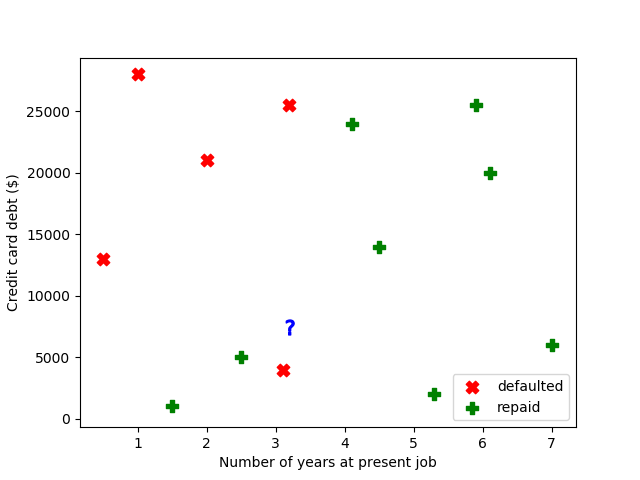
\includegraphics[width=0.9\textwidth]{bank_training.png}
\caption{Training data for a bank's home mortgage operations.}
\label{bank_training}
\end{figure}

\index{Mr.~Blue Question Mark}
Now suppose Mr.~Blue Question Mark walks in. Should we approve his loan
application? A 1-NN classifier would say \textit{no}, since the closest data
point to the blue question mark is a red X. A 3-NN classifier, on the other
hand, would say \textit{yes}, since if we take the three nearest neighbors of
the question mark, we get two greens and one red. (See
Figure~\ref{bank_training_13nn}.)

\begin{figure}[ht]
\centering
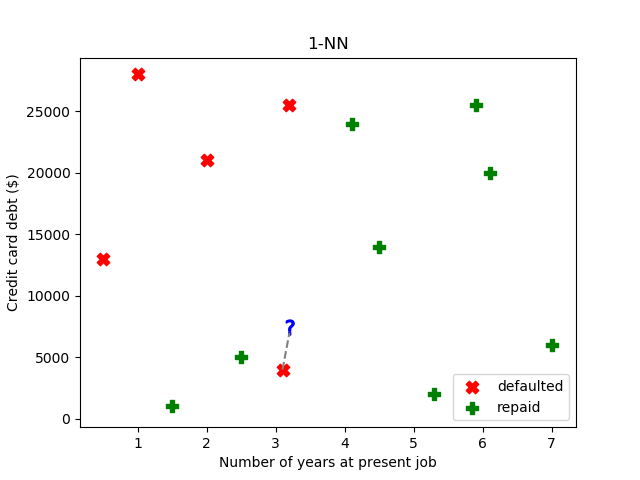
\includegraphics[width=0.48\textwidth]{bank_training_1nn.png} \ 
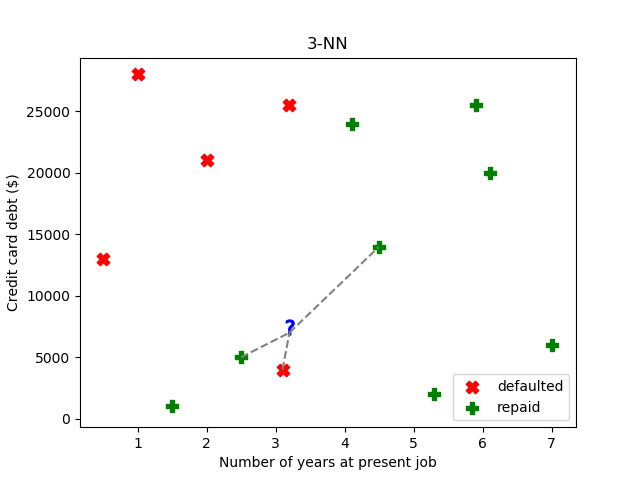
\includegraphics[width=0.48\textwidth]{bank_training_3nn.png}
\caption{The 1, and 3, ``closest'' points to our mystery man.}
\label{bank_training_13nn}
\end{figure}

\section{Distance measures}

\index{distance measure}
\index{Euclidean distance}
\index{Pythagorean Theorem}
\index{straight-line distance}
\index{crow-flies distance}

Much hinges on the question of \textit{closeness}. What do we mean when we say
two data points are ``close'' together? There are some options here, many of
which are common sense. The approach we used above was to take the ordinary
\textit{Euclidean distance}, also called the ``straight-line distance'' (or
``crow-flies distance'') between the data points. We just use the Pythagorean
Theorem where each feature is plotted on an axis. And in fact this is the most
common choice.

You probably remember the formula for the distance between two points in a
plane. Less well known is that the Pythagorean formula works \textit{in any
number of dimensions}. In other words, if I have one $n$-dimensional data point
whose values are $(x_1, x_2, x_3, ..., x_n)$ and another whose are $(y_1, y_2,
y_3, ..., y_n)$, the distance between them is:

\vspace{-.15in}
\begin{align*}
d = \sqrt{(x_1-y_1)^2 + (x_2-y_2)^2 + (x_3-y_3)^2 + \dots + (x_n-y_n)^2}
\end{align*}
\vspace{-.15in}

You can't visualize more than three dimensions (and most people can do only
two), but you can compute it, and you get a perfectly sensible number.

\index{distance measure}
\index{taxicab distance}
\index{Manhattan distance}
This isn't the only approach people use. In general, we can use any
\textbf{distance measure} (or ``distance function,'' or ``distance metric'')
that assigns a numerical ``distance'' value to any two points. To be valid, a
distance measure must simply satisfy certain common sense
rules.\footnote{Including: the distance between two points must always be
greater than or equal to 0; the distance from $x$ to $y$ must be the same as
the distance from $y$ to $x$; and the distance from $x$ to $z$ must not be any
greater than the distance from $x$ to $y$ to $z$ (the ``triangle
inequality.'')} Another common choice is the \textbf{Manhattan distance} (or
``taxicab distance'') which is essentially the shortest path between the two
points that doesn't travel diagonally (\textit{i.e.}, the path only travels
along axes.)

\section{Feature standardization}

Now I actually did something sneaky to you with the bank example. When I showed
you the plots, I calculated the crow-flies distances to Mr.~Blue Question Mark
\textit{as they appeared on the page}. But if you look at the scales of those
axes, you'll realize I didn't compute them right! These variables are on vastly
different scales. In terms of absolute differences, the amount of credit card
debt, measured in the tens of thousands, completely overwhelms the work
history, which is at most a few decades. Taking the straightforward Euclidean
distance between two people, then, would actually be quite a blunder: clearly a
difference of \$50 of credit card debt isn't nearly as significant as a
difference of 50 years in seniority!

To make this concrete, the underlying data for Figures~\ref{bank_training} and
\ref{bank_training_13nn} is here:

\begin{Verbatim}[fontsize=\small,samepage=true,frame=single,framesep=3mm]
print(bank)
\end{Verbatim}
\vspace{-.2in}

\begin{Verbatim}[fontsize=\small,samepage=true,frame=leftline,framesep=5mm,framerule=1mm]
                       num_yrs  cc_debt  default
                    0      1.0    28000      yes
                    1      0.5    13000      yes
                    2      1.5     1000       no
                    3      2.0    21000      yes
                    4      2.5     5000       no
                    5      3.1     4000      yes
                    6      3.2    25500      yes
                    7      4.1    24000       no
                    8      4.5    14000       no
                    9      5.3     2000       no
                    10     5.9    25500       no
                    11     6.1    20000       no
                    12     7.0     6000       no
                    13     3.2     7500    maybe
\end{Verbatim}

Let's compute the Euclidean distance from each of the points to Mr.~Blue
Question Mark (row \#13), and sort by that new column (remember that in Python, 
\texttt{**} is used for ``to-the-power-of''):

\index{sqrt@\texttt{sqrt()} (NumPy)}

\begin{Verbatim}[fontsize=\small,samepage=true,frame=single,framesep=3mm]
pts_dist = np.array([])
for row in bank.itertuples():
    pts_dist = np.append(pts_dist,
        np.sqrt((row.cc_debt - 7500)**2 + (row.num_yrs - 3.2)**2))
bank['dist'] = pts_dist
print(bank.sort_values('dist'))
\end{Verbatim}
\vspace{-.2in}

\begin{Verbatim}[fontsize=\small,samepage=true,frame=leftline,framesep=5mm,framerule=1mm]
                 num_yrs  cc_debt  default          dist
            13       3.2     7500    maybe      0.000000
            12       7.0     6000       no   1500.004813
            4        2.5     5000       no   2500.000098
            5        3.1     4000      yes   3500.000001
            9        5.3     2000       no   5500.000401
            1        0.5    13000      yes   5500.000663
            8        4.5    14000       no   6500.000130
            2        1.5     1000       no   6500.000222
            11       6.1    20000       no  12500.000336
            3        2.0    21000      yes  13500.000053
            7        4.1    24000       no  16500.000025
            6        3.2    25500      yes  18000.000000
            10       5.9    25500       no  18000.000202
            0        1.0    28000      yes  20500.000118
\end{Verbatim}

It's madness. The ``closest'' point to Mr.~Blue is the one with a
\texttt{num\_yrs} of 7 and a \texttt{cc\_debt} of 6000...the green point that's
pegged all the way to the right side of the plot! (See
Figure~\ref{bank_training}.)

If you think it through, you'll realize why. Moving left-or-right on this plot
is cheap; it's differences in \textit{vertical} position that generate large
distances. The far-right green plus really \textit{is} very close to Mr.~Blue,
because her credit card debt is very close to his (\$6,000 vs. \$7,500). Her 7
years of consecutive work history compared to his 3.2 just isn't a factor,
because it's measured in single digits.

\index{standardization}
\index{normalized (variable)}
\index{Z-score}

This is a very common issue with data sets, and fortunately, there's an easy
way around it. Instead of using the absolute numbers in our Pythagorean formula
calculation (or Manhattan distance calculation, or whatever), we first
\textbf{transform} our features so they are all \textbf{standardized} (or
``\textbf{Z-score normalized}\footnote{This definition of the term
``normalized'' has nothing to do with the normalization of data sets we learned
about in Sections~\ref{normalized} and \ref{normalized2}, btw.}.'') All we have
to do is take each feature, and:

\begin{compactenum}
\item subtract its mean from each point, then
\item divide each point by its standard deviation.
\end{compactenum}

This puts all features on the same level playing field, so to speak. If you
remember from your stats class, what we've done is compute the \textbf{Z-score}
for each data point: the number of standard deviations above (or below) the
mean it is. Now no feature gets an advantage in the distance calculation over
any other feature, even if they're on wildly different scales: 2.5 standard
deviations is 2.5 standard deviations, no matter what the underlying units.

Here's code to do that with the bank example:

\begin{Verbatim}[fontsize=\small,samepage=true,frame=single,framesep=3mm]
def zscores(arr):
    return (arr - arr.mean()) / arr.std()

bank.cc_debt = zscores(bank.cc_debt)
bank.num_yrs = zscores(bank.num_yrs)
\end{Verbatim}

Now, if we compute distances with these Z-scores, instead of the raw values, we
get something that looks much more reasonable:

\begin{Verbatim}[fontsize=\small,samepage=true,frame=single,framesep=3mm]
zscore_dist = np.array([])
for row in bank.itertuples():
    zscore_dist = np.append(zscore_dist,
        np.sqrt((row.cc_debt - bank.iloc[len(bank)-1].cc_debt)**2 +
            (row.num_yrs - bank.iloc[len(bank)-1].num_yrs)**2))
bank['dist'] = zscore_dist
print(bank.sort_values('dist'))
\end{Verbatim}
\vspace{-.2in}

\begin{Verbatim}[fontsize=\small,samepage=true,frame=leftline,framesep=5mm,framerule=1mm]
                 num_yrs    cc_debt  default      dist
            13 -0.181877  -0.667388    maybe  0.000000
            5  -0.231804  -1.024786      yes  0.360869
            4  -0.531366  -0.922673       no  0.432797
            8   0.467174  -0.003647       no  0.928342
            2  -1.030636  -1.331128       no  1.077471
            9   0.866590  -1.229014       no  1.189415
            1  -1.529906  -0.105761      yes  1.460345
            3  -0.781001   0.711151      yes  1.503103
            7   0.267466   1.017493       no  1.743769
            6  -0.181877   1.170664      yes  1.838051
            12  1.715350  -0.820559       no  1.903400
            11  1.266006   0.609037       no  1.930188
            10  1.166152   1.170664       no  2.279389
            0  -1.280271   1.425948      yes  2.364006
\end{Verbatim}

The data is plotted on Z-score normalized axes in
Figure~\ref{bank_training_zscore}. As you can see, the nearest neighbor to
Mr.~Blue is the point .023 standard deviations lower than the mean job
seniority, and 1.02 standard deviations lower than the mean credit card debt,
which is precisely the red X nearest to the question mark.

\begin{figure}[ht]
\centering
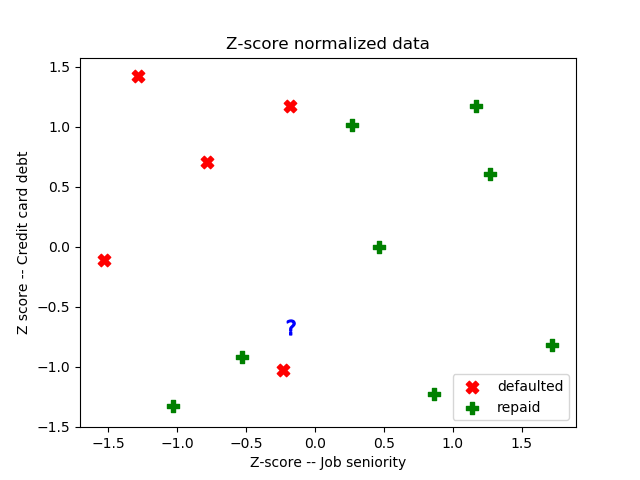
\includegraphics[width=0.9\textwidth]{bank_training_zscore.png}
\caption{Both variables have been Z-score normalized (note the axis scales)!}
\label{bank_training_zscore}
\end{figure}


\section{Categorical features}

Now what do we do if our features are categorical? We can just make them
numerical, but in a principled way. If we have a binary feature, with only two
possible values -- \texttt{public}/\texttt{private},
\texttt{collegeGraduate}/\texttt{notACollegeGraduate} -- it's easy: we just
assign one number (say, ``1'') to one value and another (``2'') to the other
one. Now we've turned a categorical column of
\texttt{employed}-or-\texttt{unemployed}'s into a numeric column of 1-or-2's,
which lets us compute Z-scores and distance measures as we did above.

\index{baseball}
\index{football}
\index{lacrosse}

With more than two possible values, though, you have to be careful. Consider a
feature whose three values are ``\texttt{baseball},'' ``\texttt{football},''
and ``\texttt{lacrosse}.'' Many people might unsuspectingly assign the numbers
1, 2, and 3 to these values and then treat the feature as a numeric one. But
you can't do this. Here's why: assuming the original values were on a
categorical/nominal scale (recall the ``Scales of Measure'' chapter from Volume
I of this series), converting them to numbers in a simpleminded fashion like
this \textit{imposes an interval scale where none exists.}

Think about it. A person whose favorite sport is baseball isn't any
\textit{more} like a football fan than she is like a lacrosse fan. Yet if we
turn \texttt{baseball} into 1, \texttt{football} into 2, and \texttt{lacrosse}
into 3, that's exactly what our kNN classifier is going to think. It will view
baseball fans and lacrosse fans as ``further apart'' because after all, 3 minus
1 is 2.

\index{one-hot encoding}

In order to avoid biasing the classifier with this non-information, we use a
technique called \textbf{one-hot encoding}. We turn each categorical feature
into a whole \textit{set} of binary features, one for each value. So instead of
a \texttt{sport} feature with values \texttt{baseball}, \texttt{football}, and
\texttt{lacrosse}, we use \textit{three} features -- called \texttt{baseball},
\texttt{football}, and \texttt{lacrosse} -- each with values of 0 or 1.
Example:

\begin{center}
\footnotesize
\begin{tabular}{|c|c|c|}
\hline
age & edLevel & sport \\
\hline
37 & HS & football \\
41 & college & baseball \\
19 & college & football \\
22 & college & lacrosse \\
\hline
\end{tabular}
\quad
{\Huge $\Rightarrow$}
\quad
\begin{tabular}{|c|c|c|c|c|c|}
\hline
age & HS & college & football & baseball & lacrosse \\
\hline
37 & 1 & 0 & 1 & 0 & 0 \\
41 & 0 & 1 & 0 & 1 & 0 \\
19 & 0 & 1 & 1 & 0 & 0 \\
22 & 0 & 1 & 0 & 0 & 1 \\
\hline
\end{tabular}
\end{center}

\index{wide form}
\index{long form}

Perhaps you can see why it's called ``one-hot'' encoding: each row has exactly
one ``hot'' (\textit{i.e.}, 1) entry for each of the one-hotted features.
Specifically, every row has either a 0 for \texttt{HS} and a 1 for
\texttt{college}, or vice versa; and every row has a 1 for exactly \textit{one}
of \texttt{football}, \texttt{baseball}, and \texttt{lacrosse}, and 0 for the
other two. This is sort of like going from \textbf{long form} to \textbf{wide
form} data, if you think about it.

\index{scikit-learn@\texttt{scikit-learn} (package)}
\index{OneHotEncoder@\texttt{OneHotEncoder.fit\_transform()}}
\index{fit\_transform@\texttt{fit\_transform()}}
\index{sparse@\texttt{sparse=False} (\texttt{OneHotEncoder})}

You can use \texttt{np.where()} function to create one-hot features, or you
might find the \texttt{scikit-learn} package's
\texttt{OneHotEncoder.fit\_transform()} function helpful. It's a little weird;
when you create your \texttt{OneHotEncoder}, you have to pass it an argument of
``\texttt{sparse=False}'' if you want it to work the way you expect.

\index{import@\texttt{import}}
\index{double boxies@``double boxies''}
\index{[]@\texttt{[]} (boxies)}

\begin{Verbatim}[fontsize=\small,samepage=true,frame=single,framesep=3mm]
from sklearn.preprocessing import OneHotEncoder

ohe = OneHotEncoder(sparse=False)
onehot_features = ohe.fit_transform(df[['edLevel','sport']])
\end{Verbatim}

Careful: although this function takes a \texttt{DataFrame} as input, it returns
a \texttt{NumPy} array as output:

\begin{Verbatim}[fontsize=\small,samepage=true,frame=single,framesep=3mm]
print(df[['edLevel','sport']])
\end{Verbatim}
\vspace{-.3in}

\begin{Verbatim}[fontsize=\small,samepage=true,frame=leftline,framesep=5mm,framerule=1mm]
   edLevel     sport
0       HS  football
1  college  baseball
2  college  football
3  college  lacrosse
3    lacrosse
Name: sport, dtype: object
\end{Verbatim}

\begin{Verbatim}[fontsize=\small,samepage=true,frame=single,framesep=3mm]
print(onehot_features)
\end{Verbatim}
\vspace{-.3in}

\begin{Verbatim}[fontsize=\small,samepage=true,frame=leftline,framesep=5mm,framerule=1mm]
[[1. 0. 0. 1. 0.]
 [0. 1. 1. 0. 0.]
 [0. 1. 0. 1. 0.]
 [0. 1. 0. 0. 1.]]
\end{Verbatim}

\medskip
If you want these columns back in your \texttt{DataFrame}, you'll have to stick
them back in there:

\begin{Verbatim}[fontsize=\small,samepage=true,frame=single,framesep=3mm]
df['HS'] = onehot_features[:,0]
df['college'] = onehot_features[:,1]
df['baseball'] = onehot_features[:,2]
df['football'] = onehot_features[:,3]
df['lacrosse'] = onehot_features[:,4]
df = df.drop(['edLevel','sport'],axis=1)

print(df)
\end{Verbatim}
\vspace{-.3in}

\begin{Verbatim}[fontsize=\small,samepage=true,frame=leftline,framesep=5mm,framerule=1mm]
   age   HS  college  baseball  football  lacrosse
0   37  1.0      0.0       0.0       1.0       0.0
1   41  0.0      1.0       1.0       0.0       0.0
2   19  0.0      1.0       0.0       1.0       0.0
3   22  0.0      1.0       0.0       0.0       1.0
\end{Verbatim}

But as we'll see in the next chapter, the array itself is ready-made for
\texttt{scikit-learn}'s powerful classifier implementations. Stay tuned.
            

\chapter{ML classifiers: kNN (2 of 2)}

Last chapter gave the theory of kNN classifiers. Now how would we code one in
Python?

Conceptually it's pretty easy. We'll want to Z-score normalize everything
first, of course. Then, for a new, unlabeled data point, we'll compute the
``distance'' (via whichever measure we choose) between it and every point in
the training set. Then, we sort these points by distance, choose the $k$ with
the smallest distance, and take a majority vote.

\index{synthetic data set}

We'll use our bank loan example, but with a lot more rows. Let's synthesize a
data set real quick:

\begin{Verbatim}[fontsize=\footnotesize,samepage=true,frame=single,framesep=3mm]
NUM = 1000
default = np.random.choice(['yes','no'], p=[.3,.7], size=NUM)
cc_debt = np.where(default == 'yes',
    np.random.normal(12000, 4000, NUM).clip(0, 40000).astype(int),
    np.random.normal(7000, 3000, NUM).clip(0, 40000).astype(int))
num_yrs = np.where(default == 'yes',
    np.random.uniform(0, 10, NUM).round(1),
    np.random.uniform(2, 12, NUM).round(1))
bank = pd.DataFrame({'cc_debt':cc_debt, 'num_yrs':num_yrs,
    'default':default})[['cc_debt','num_yrs','default']]
\end{Verbatim}

In our simplistic, synthesized world, we're assuming that 30\% of our 1,000
people default on their loans, and that those who do tend to have a bit more
credit card debt and somewhat fewer years at their current job. The resulting
\texttt{DataFrame} looks like this:

\begin{Verbatim}[fontsize=\scriptsize,samepage=true,frame=leftline,framesep=5mm,framerule=1mm]
                     cc_debt  num_yrs default
                0       7318      8.3     yes
                1       2524      9.5      no
                2      14866      5.1     yes
                3      10611      5.4      no
                4       9897      3.7      no
                ..       ...      ...     ...
                995     5136      6.8      no
                996     7594     11.4      no
                997     7851      7.1      no
                998        0      7.5      no
                999    13697      7.0     yes
                [1000 rows x 3 columns]
\end{Verbatim}

and we can plot it: 
\index{grouped scatter plot}
\index{scatter plot!grouped}

\begin{Verbatim}[fontsize=\footnotesize,samepage=true,frame=single,framesep=3mm]
sns.pairplot(data=bank, x_vars=['num_yrs'], y_vars=['cc_debt'], hue='default')
\end{Verbatim}

to get the grouped scatter plot in Figure~\ref{synthesized_bank}.

\begin{figure}[ht]
\centering
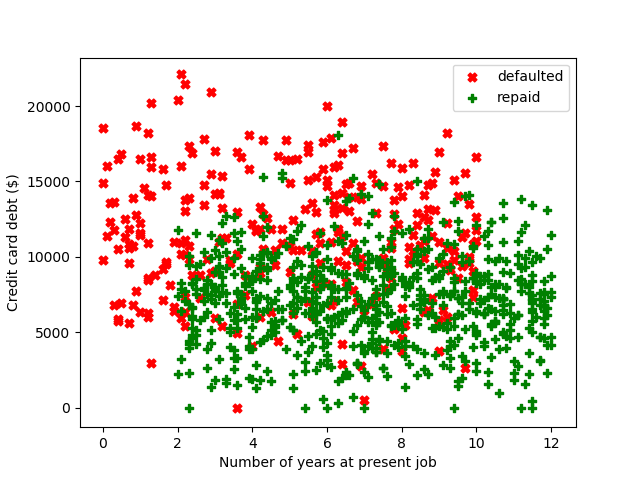
\includegraphics[width=0.85\textwidth]{synthesized_bank.png}
\caption{Synthesized bank data.}
\label{synthesized_bank}
\end{figure}

\section{Coding kNN by hand}

\index{standardization}
\index{normalized (variable)}
\index{Z-score}

To use this as training data, we'll Z-score normalize the features. We also
need to Z-score the \textit{new} data points that come in to be classified,
though, so we'd better remember the mean and standard deviation of each
feature.

\begin{Verbatim}[fontsize=\small,samepage=true,frame=single,framesep=3mm]
def zscores(arr):
    return (arr - arr.mean()) / arr.std()

cc_debt_mean = bank.cc_debt.mean()
cc_debt_std = bank.cc_debt.std()
num_yrs_mean = bank.num_yrs.mean()
num_yrs_std = bank.num_yrs.std()

bank.cc_debt = zscores(bank.cc_debt)
bank.num_yrs = zscores(bank.num_yrs)
\end{Verbatim}
\vspace{-.2in}

\begin{Verbatim}[fontsize=\scriptsize,samepage=true,frame=leftline,framesep=5mm,framerule=1mm]
                  cc_debt   num_yrs default
            0    1.321445  0.152280     yes
            1    0.877662 -0.407452      no
            2    0.150633 -1.000109     yes
            3    2.152262 -1.790319     yes
            4    0.927766  1.238819      no
            ..        ...       ...     ...
            995 -1.450414 -0.670855      no
            996 -0.777325  0.415683      no
            997 -0.172235  0.942490      no
            998  0.385818  0.316907     yes
            999 -0.669958  1.600998      no
\end{Verbatim}

\index{predict@\texttt{predict()}}
\index{dist@\texttt{dist()}}

Now let's write a function called \texttt{predict()} (to match the name we used
in Chapters~\ref{ch:naiveBayes2} and ~\ref{ch:naiveBayes3}) which will make a
loan-default prediction for a new applicant. We'll also write a \texttt{dist()}
(for ``distance'') function to help it do its job.

\index{Euclidean distance}
\index{Pythagorean Theorem}

\begin{Verbatim}[fontsize=\small,samepage=true,frame=single,framesep=3mm]
def dist(x,y):
    return np.sqrt((x[0]-y[0])**2 + (x[1]-y[1])**2)
\end{Verbatim}

We're using Euclidean distance here (Pythagorean Theorem), obviously. Our
\texttt{predict()} will call this \texttt{dist()} function for every point to
determine that point's Euclidean distance from our test point. Then, it will
sort those by distance, pick the top $k$, and choose the majority:

\begin{Verbatim}[fontsize=\small,samepage=true,frame=single,framesep=3mm]
def predict(cc_debt, num_yrs, k):
    bank['dists'] = dist([bank.cc_debt, bank.num_yrs],
        [(cc_debt - cc_debt_mean) / cc_debt_std,
        (num_yrs - num_yrs_mean) / num_yrs_std])
    k_closest_pts = bank.sort_values('dists').iloc[0:k]
    return k_closest_pts.default.value_counts().index[0]
\end{Verbatim}

Can you understand what this function is doing?

First, notice that because of the magic of Pandas broadcasting operations, we
don't even need a loop. The first line of the function calls \texttt{dist()} a
grand total of once, giving it a list of the entire training data's x-values
and y-values as the first argument, and then the new point's x-value and
y-value (both Z-score normalized) as the second argument. Pretty slick!

Then walk through how the majority rule is applied. The variable
``\texttt{k\_closest\_pts},'' after the next line, will be a \texttt{DataFrame}
that looks like so:

\begin{Verbatim}[fontsize=\small,samepage=true,frame=leftline,framesep=5mm,framerule=1mm]
              cc_debt   num_yrs default     dists
        651 -0.058795 -0.720668     yes  0.101662
        254 -0.010493 -0.720668     yes  0.105948
        515  0.057728 -0.854746      no  0.106971
        384  0.076899 -0.821226      no  0.120755
        418 -0.147929 -0.754187     yes  0.123796
        873  0.087356 -0.821226     yes  0.131212
        672 -0.061782 -0.955304      no  0.135271
\end{Verbatim}

\index{value\_counts@\texttt{.value\_counts()} (Pandas)}

(This assumes we passed a value of 7 for the \texttt{k} argument to
\texttt{predict()} and are thus doing 7-NN.) Notice how the rows are ordered in
decreasing distance from our new data point. In the final line of the function,
we take the \texttt{.value\_counts()} of this \texttt{DataFrame}'s
\texttt{default} column. This produces an intermediate value like:

\begin{Verbatim}[fontsize=\small,samepage=true,frame=leftline,framesep=5mm,framerule=1mm]
        yes    4
        no     3
        Name: default, dtype: int64
\end{Verbatim}

and when we take \texttt{.index[0]} of that, we get the label with the
highest value count. In this case, it's ``\texttt{yes},'' so let's not give a
loan to that guy.

\subsection{Evaluating the hand-coded version}

We can measure how well this classifier performs using essentially the same
code we wrote back on p.~\pageref{evaluateNBcode}:

\begin{Verbatim}[fontsize=\small,samepage=true,frame=single,framesep=3mm]
num_correct = 0
for i in range(len(test)):
    row = test.iloc[i]
    p = predict(row['cc_debt'], row['num_yrs'], 3)
    if p == row['default']:
        num_correct += 1
print("We got {}% correct.".format(num_correct/len(test)*100))
\end{Verbatim}
\vspace{-.2in}

\begin{Verbatim}[fontsize=\small,samepage=true,frame=leftline,framesep=5mm,framerule=1mm]
We got 73.667% correct.
\end{Verbatim}

Not that great, but looking again at Figure~\ref{synthesized_bank}
(p.~\pageref{synthesized_bank}) you can see why! There's a huge region in that
space where defaulters and non-defaulters have about the same prominence. For
new points that fall in the midst of that morass, we're only guessing. In a
region like that, no classifier is going to have much of a chance.

%\index{scikit-learn@\texttt{scikit-learn} (package)}
%\section{The \texttt{scikit-learn} library}
%
%
%
%Let's use the scikit-learn library to compare 3-NN with Naive Bayes. First, we
%load the data and split it randomly into training and test sets:
%
%\begin{Verbatim}[fontsize=\footnotesize,samepage=true,frame=single]
%w = pd.read_csv("warriors.csv")
%train = w.sample(frac=.7)
%test = w.drop(train.index)
%\end{Verbatim}
%\normalsize
%
%\vspace{-.05in}
%Next, we one-hot encode the features (all of which are categorical):
%\vspace{-.1in}
%\begin{Verbatim}[fontsize=\footnotesize,samepage=true,frame=single]
%def one_hot_this_puppy(df):
%    lb = LabelBinarizer()
%    lightsaber = lb.fit_transform(df.lightsaber)
%    height = lb.fit_transform(df.height)
%    beard = lb.fit_transform(df.beard)
%    demeanor = lb.fit_transform(df.demeanor)
%    return np.concatenate([lightsaber, height, beard, demeanor], axis=1)
%
%train_features = one_hot_this_puppy(train)
%test_features = one_hot_this_puppy(test)
%\end{Verbatim}
%\normalsize
%
%\vspace{-.05in}
%We'll call scikit-learn's Naive Bayes implementation:
%\vspace{-.15in}
%
%\begin{Verbatim}[fontsize=\footnotesize,samepage=true,frame=single]
%from sklearn.naive_bayes import MultinomialNB
%naive_bayes = MultinomialNB()
%naive_bayes.fit(train_features,train.type.as_matrix())
%nb_predictions = naive_bayes.predict(test_features)
%\end{Verbatim}
%\normalsize
%
%\vspace{-.05in}
%and its KNN implementation:
%\vspace{-.15in}
%
%\begin{Verbatim}[fontsize=\footnotesize,samepage=true,frame=single]
%from sklearn.neighbors import KNeighborsClassifier
%knn = KNeighborsClassifier(n_neighbors=3)
%knn.fit(train_features, train.type.as_matrix())
%knn_predictions = knn.predict(test_features)
%\end{Verbatim}
%\normalsize
%
%\vspace{-.05in}
%Finally, print the results:
%\vspace{-.15in}
%
%\begin{Verbatim}[fontsize=\footnotesize,samepage=true,frame=single]
%>>> print("Naive Bayes got {:.2f}% correct.".format(
%        sum(nb_predictions == test.type)/len(test)*100))
%>>> print("kNN(3) got {:.2f}% correct.".format(
%        sum(knn_predictions == test.type)/len(test)*100))
%    Naive Bayes got 79.00% correct.
%    kNN(3) got 86.33% correct.
%\end{Verbatim}
%\normalsize
%
%Pretty close, but for this data set, 3-NN has the edge.
%
%\subsection{Comparing kNN with Naive Bayes}
%
%\pagebreak
%It's also illustrative to examine \textit{which} points Naive Bayes called
%correctly but 3-NN missed, and vice versa.
%
%\begin{Verbatim}[fontsize=\footnotesize,samepage=true,frame=single]
%nb_right = []
%knn_right = []
%for i in range(len(nb_predictions)):
%    if nb_predictions[i] == test.type.iloc[i] != knn_predictions[i]:
%        nb_right.append(i)
%    if nb_predictions[i] != test.type.iloc[i] == knn_predictions[i]:
%        knn_right.append(i)
%nb_right_examples = test.iloc[nb_right]
%knn_right_examples = test.iloc[knn_right]
%
%>>> print("Naive Bayes got these right:")
%>>> print(nb_right_examples)
%>>> print("\nkNN got these right:")
%>>> print(knn_right_examples)
%\end{Verbatim}
%
%\begin{multicols}{2}
%\begin{Verbatim}[fontsize=\scriptsize,samepage=true,frame=none]
%Naive Bayes got these right:
%    beard  height  demeanor lightsaber  type
%7      no  medium      calm      green  Jedi
%63     no   short  menacing      green  Jedi
%116    no  medium      calm      green  Jedi
%154    no  medium      calm      green  Jedi
%185    no   short  menacing      green  Jedi
%190    no   short  menacing      green  Jedi
%279    no  medium      calm       blue  Jedi
%600    no  medium      calm       blue  Jedi
%827    no   short  menacing      green  Jedi
%842    no   short  menacing      green  Jedi
%909    no   short  menacing      green  Jedi
%\end{Verbatim}
%\columnbreak
%\begin{Verbatim}[fontsize=\scriptsize,samepage=true,frame=none]
%kNN got these right:
%    beard  height  demeanor lightsaber  type
%1      no   short      calm       blue  Sith
%33     no   short      calm       blue  Sith
%55     no   short      calm       blue  Sith
%94     no  medium      calm      green  Sith
%106    no   short      calm       blue  Sith
%254    no   short  menacing      green  Sith
%283    no   short      calm       blue  Sith
%366    no  medium      calm       blue  Sith
%380    no  medium      calm      green  Sith
%385    no  medium      calm       blue  Sith
%431    no   short      calm       blue  Sith
%468    no   short      calm       blue  Sith
%570    no   short      calm       blue  Sith
%581    no   short      calm       blue  Sith
%599    no   short      calm      green  Sith
%686    no  medium      calm      green  Sith
%713    no  medium      calm       blue  Sith
%733    no   short      calm       blue  Sith
%743    no  medium      calm       blue  Sith
%815    no   short  menacing      green  Sith
%870    no   short      calm       blue  Sith
%931    no  medium      calm       blue  Sith
%966    no  medium      calm      green  Sith
%991    no  medium      calm       blue  Sith
%\end{Verbatim}
%\end{multicols}
%\normalsize
%
%Interestingly, all of Naive Bayes's errors were in one direction (incorrect
%\texttt{Jedi} call) and all 3-NN's in the other. Naive Bayes seems to have the
%most trouble with clean-shaven, calm, non-red-lightsabered Sith Lords. It
%tends to call them ``Jedi,'' because two of the features --
%\texttt{demeanor=calm} and \texttt{lightsaber=blue/green} -- are highly
%\texttt{Jedi}-indicative. When factored in with just one
%\texttt{Sith}-indicative feature (\texttt{beard=no}), those two features
%overcome the third and tilt the Naive Bayes scales (incorrectly) towards Jedi.
%3NN is able to pick out these \texttt{Sith} from the \texttt{Jedi} masses.
%
%\subsection{Varying $k$}
%
%One question that arises is: ``what's the
%optimal value of $k$?'' It may or may not surprise you to learn that there's no
%easy answer to this, and that it varies widely by data set and in fact even by
%the training set chosen.
%
%Here's some code to try all (odd) values of $k$ between 1 and 301:
%\begin{Verbatim}[fontsize=\footnotesize,samepage=true,frame=single]
%corrects_train = []
%corrects_test = []
%for k in np.arange(1,301,2):
%    knn = KNeighborsClassifier(n_neighbors=k)
%    knn.fit(train_features, train.type.as_matrix())
%    knn_predictions_train = knn.predict(train_features)
%    knn_predictions_test = knn.predict(test_features)
%    corrects_train.append(sum(knn_predictions_train == train.type)/len(train)*100)
%    corrects_test.append(sum(knn_predictions_test == test.type)/len(test)*100)
%\end{Verbatim}
%\normalsize
%
%The resulting plot is in Figure~\ref{fig:varyingK}. The performance on the
%training data is \textit{usually} better, as expected, although you'll see
%some values of $k$ here in the 80-100 range where paradoxically that's not
%true. More importantly, you'll notice that the line shows no simple pattern.
%Very low numbers are good, and then performance tails off...but then it goes
%back up again when $k$ is around 100 or so. Moreover, \textit{the apparent
%optimal choice of k depends on the training set.}
%
%\begin{figure}
%\centering
%\includegraphics[width=0.9\textwidth]{k_vs_performance.pdf}
%\caption{Correct classification rate as a function of $k$.}
%\label{fig:varyingK}
%\end{figure}
%
%Figure~\ref{fig:varyingTrainingSet} has some more results from the same code,
%with different randomly-chosen training sets. We see some similarities here,
%but by no means perfect uniformity. This is because a kNN classifier is a
%high-variance classifier (especially for low $k$), as described in the next
%section.
%
%\begin{figure}
%\centering
%\includegraphics[width=0.31\textwidth]{k_vs_performance1.pdf}
%\includegraphics[width=0.31\textwidth]{k_vs_performance2.pdf}
%\includegraphics[width=0.31\textwidth]{k_vs_performance3.pdf}
%\caption{Correct classification rate vs.~$k$, for different training sets.}
%\label{fig:varyingTrainingSet}
%\end{figure}
%
%
%\section{The ``Bias-Variance Tradeoff''}
%
%One of the most deep and fundamental principles of machine learning goes by
%the name of \textbf{the bias-variance tradeoff}. It's a version of the ``no
%free lunch'' principle: classifiers that possess one advantage inherently have
%a counteracting disadvantage.
%
%Here are the two key terms:
%
%\begin{itemize}
%\itemsep.1em
%\item \textbf{bias}\footnote{Tip: when thinking about this topic, try to erase the previous definitions you
%have for the word ``\textit{bias}'' that you have running around in your brain.
%They probably don't apply. When I think of ``bias'' I think of a systematic
%propensity to err \textit{in a particular direction}. Like, ``you're biased
%towards thinking people are shorter than they are, because you're tall.'' But
%\textit{bias} here just means ``being `off' in general, in whatever direction,
%and probably not the same direction each time.''}
% -- the degree to which a model is expected to misclassify
%items, even those in its own training set, because it just can't ``bend'' 
%enough to catch all the detail.
%\item \textbf{variance} -- the degree to which a model will differ based on
%the particular training set that is chosen, because it ``bends'' too much to
%try and catch every data point.
%\end{itemize}
%
%The basic theory is as follows. Suppose you have a very simple classifier that
%tries to identify a single, smooth, perfectly straight line separating the
%data points. Maybe our model says ``just use the \texttt{lightsaber} feature
%by itself, and call `\texttt{Jedi}' or `\texttt{Sith}' based on whether the
%test point's lightsaber value is more typical of the \texttt{Jedi} Knights and
%\texttt{Sith} Lords in the data set.
%
%This simple classifier can be said to have \textbf{low variance}. Why? Because
%if, instead of those particular 714 training points chosen from the
%population, I had sampled a different 714 training points, \textit{the
%classification decisions I would make on new data would be about the same.} To
%see why this is the case, consider how different the training sets would have
%to me in order for me to make any \textit{different} decisions. Let's say my
%original 714 training points had:
%
%\begin{center}
%\begin{Verbatim}[fontsize=\small,samepage=true,frame=none]
%        Jedi    Sith
%red       17      85
%blue     283      28
%green    299       2
%\end{Verbatim}
%\end{center}
%
%for their lightsaber colors. Clearly, my very simply classifier is going to
%predict \texttt{Sith} for any \texttt{red}-lightsaber wielder and
%\texttt{Jedi} for anyone else. Now if I had collected a different training
%set, the numbers above would be different, but they would have to be a
%\textit{lot} different to change any of my future predictions. I'd have to
%have an additional 68 \texttt{red} \texttt{Jedi}, for instance, or 255
%additional \texttt{blue} \texttt{Sith}, or a whopping 297 additional
%\texttt{green} \texttt{Sith}, without any increase in the other class. Not
%likely.
%
%That's the bright side. On the dark side, by classifying points in this way,
%this simple model is going to get a lot of data points wrong: $17+28+2=47$
%points incorrect \textit{in its own training set}, in fact. This mean it's a
%pretty \textbf{high bias} classifier.
%
%It's a tradeoff. In exchange for being virtually immune to the idiosyncrasies
%in the training sample, we've sacrificed some precision.
%
%The other extreme can be seen by visualizing a 1-NN classifier. Now, for a
%future data point, we're going to find the single nearest neighbor to it in
%our training set, and call \texttt{Jedi} or \texttt{Sith} accordingly. This is
%very \textbf{low bias} -- we're guaranteed to get every training point
%correct, in fact!\footnote{Unless there are data points with identical feature
%values but different labels, in which case whatcha gonna do.} But it is also
%very \textbf{high variance}: a different training set will result in many,
%many different classifications. Our classifier has essentially memorized a
%zillion individual examples, and will regurgitate all that intricate detail on
%command. But had we gotten a different random sample, the ``single nearest
%neighbor'' to a test point would have been totally different, and might result
%in a different classification.
%     
%There are formulas you can use to work out quantitatively what the estimated
%bias and variance are for a classifier. But I think this dichotomy is more
%important from a conceptual perspective. The main lesson is: the more your
%classifier ``bends'' (\textit{i.e.}, has a very wiggly and unpredictable
%boundary between its ranges of predicted classes) the more precise it
%potentially is in selectively labeling data points. However, this also means
%that a lot of its decisions are going to hinge on the particular data sample
%it was trained on, which means it will probably be picking up noise in
%addition to signal.
%
%
%\section{The ``Curse of Dimensionality''}
%\label{sec:curse}
%
%Another key ML principle goes by the humorous name \textbf{the curse of
%dimensionality}. It goes something like this. Suppose that in addition to
%\texttt{height}, \texttt{demeanor}, \texttt{lightsaber}, and \texttt{beard},
%we also have at our disposal many other features about Jedi \& Sith: their
%ages, salaries, home planets, personality profiles, number of traffic tickets,
%\textit{etc.} This is good news, right? It gives us more and more data to sift
%through statistically and discover correlations, right? What's not to like?
%
%Yes, this is potentially good news, but with a catch. It turns out that as we
%increase the number of features more and more (or, put another way, as we
%increase the ``dimensionality'' of the problem from our original four
%dimensions to 5, 6, 7, ..., and up into the hundreds) we have a data sparsity
%problem. In terms of kNN classifiers, you can think of it this way:
%effectively, \textit{all} the points effectively become far apart. We want to
%find the 3 (or 15, or 77) ``nearest neighbors,'' but when we have so many
%features (many of which will turn out to be irrelevant for the problem), we
%find that \textit{any} two data points will differ on a large number of them.
%Essentially, our noise swamps our signal.
%
%Another aspect of the problem concerns the amount of training data that we
%need. When we have tons of features, we need an enormous number of training
%samples in order to guarantee that we have several samples with each
%combination of values (or their ranges). In our original problem, we didn't
%need to much data to ensure that we'd have at least a few \texttt{tall},
%\texttt{green}-lightsabered, \texttt{menacing} individuals with \texttt{no}
%beard. But how many training points will we need before we have several
%\texttt{tall}, \texttt{green}-lightsabered, \texttt{menacing}, 38-year-old,
%extroverted, abstract-thinking individuals from Tatooine with 4 traffic
%tickets and \texttt{no} beard who earn 6,000 Galactic credits annually?
%Answer: a lot. And if we don't have that many, a kNN classifier trained on all
%those features is going to suffer trying to find ``people like this one'' in
%order to make a prediction.
%
%The moral to the story is that we will often need to trim our set of features,
%sometimes aggressively, if we have too many. It feels wasteful -- all this
%great data on all these people, and we're throwing it away! -- but it's the
%right thing to do. This process is called \textbf{feature selection}, and
%we'll cover it more fully in a future lesson.
%
%\vspace{.1in}
%In the meantime, here are three useful principles for avoiding the curse:
%
%\begin{itemize}
%\itemsep.1em
%\item By far the most important thing to recognize is that if you have
%additional features that are \textit{truly} (and pretty strongly) correlated
%with the target, it's okay to include them. Adding more stuff that actually
%contains useful information for prediction isn't generally a problem. The
%problem is when you add features that are largely \textit{noise}, since
%they will overwhelm the truly significant features if there are too many of
%them.
%\item A common rule of thumb is to make sure you have at least \textit{five}
%training points for each combination of feature values. (In our Jedi example,
%with three \texttt{height}s and three \texttt{lightsaber} values and two
%values for the other features, this would imply a training set of at least $(3
%\times 3 \times 2 \times 2) \times 5 = 180$ training points.)
%\item When the size of the training set becomes too low, use
%\textit{parametric} methods (like Naive Bayes or linear regression) rather
%than instance-based methods (like kNN) because they suffer less from the
%curse.
%\end{itemize}
%
%
            

\chapter{Two key ML principles}
\index{bias-variance trade-off}

\section{``The bias-variance trade-off''}

Earlier in the book (p.~\pageref{bvTradeoffLowess}) I made a reference to
something called ``the bias-variance trade-off.'' This turns out to be one of
the most important general principles in all of ML, and it's now time to look
at it in detail.

\index{no free lunch@the ``no free lunch'' principle}

The \textbf{bias-variance trade-off} is a manifestation of the ``no free
lunch'' principle. Classifiers that possess one advantage inherently have a
counteracting disadvantage. Here are the two key terms:

\begin{itemize}
\itemsep.1em

\item \textbf{bias}\footnote{Tip: when thinking about this topic, try to erase
your previous definitions for the word ``\textit{bias}'' that you have running
around in your brain. They probably don't apply. The normal meaning of the word
``bias'' implies a systematic propensity to err \textit{in a particular
direction}. Like, ``you're biased towards thinking people are shorter than they
are, because you're tall.'' But in this chapter, \textit{bias} just means
``being `off' in general, in whatever direction, and probably not the same
direction each time.''} -- the degree to which a model is expected to
misclassify items, even those in its own training set, because it just can't
``bend'' enough to catch every data point.

\item \textbf{variance} -- the degree to which a model will differ based on the
particular training set that is chosen, because it ``bends'' too much to try
and catch every data point.

\end{itemize}

\index{Sith}
\index{Jedi}
\index{security camera}
\index{spycam}

The basic theory is as follows. Suppose you have a very simple classifier that
takes 714 training points from a security camera and tries to identify a
single, smooth, perfectly straight line roughly separating Jedi from Sith.
Maybe our model says ``just use the \texttt{lightsaber} feature by itself, and
call `\texttt{Jedi}' or `\texttt{Sith}' based on whether the test point's
lightsaber value is more typical of the \texttt{Jedi} Knights or the
\texttt{Sith} Lords in the training set.''

This simple classifier can be said to have \textbf{low variance}. Why? Because
if, instead of those particular 714 training points chosen from the
population, I had sampled a different 714 training points, \textit{the
classification decisions I would make on new data would be about the same.} To
see why this is the case, consider how different the training sets would have
to be in order for me to make any \textit{different} decisions. Let's say the
lightsaber colors for my original 714 training points were:

\label{simpleClassifierTable}
\Large
\begin{center}
\begin{tabular}{|l|rr|}
\hline
& Jedi & Sith \\
\hline
red & 17 & 85 \\
blue & 283 & 28 \\
green & 299 & 2 \\
\hline
\end{tabular}
\end{center}
\normalsize

Clearly, my very simply classifier is going to predict \texttt{Sith} for
\texttt{red}-lightsaber wielders and \texttt{Jedi} for anyone else. Now if I
had collected a different training set, the numbers above would be different,
but they would have to be a \textit{lot} different to change any of my future
predictions. I'd have to have an additional 68 \texttt{red} \texttt{Jedi}, for
instance, or 255 additional \texttt{blue} \texttt{Sith}, or a whopping 297
additional \texttt{green} \texttt{Sith}. Not likely.

That's the bright side. On the dark side, by classifying points in this way,
this simple model is going to get a lot of data points wrong: $17+28+2=47$
points incorrect \textit{in its own training set}, in fact. This mean it's a
pretty \textbf{high bias} classifier.

It's a tradeoff. In exchange for being virtually immune to the idiosyncrasies
in the training sample, we've sacrificed some precision.

\index{kNN@kNN ($k$-nearest neighbors)}

The other extreme can be seen by visualizing a 1-NN classifier. When given a
new data point, 1-NN will find the \textit{single} nearest neighbor to it in
the training set, and call \texttt{Jedi} or \texttt{Sith} accordingly. This is
very \textbf{low bias} -- heck, we're guaranteed to get every training point
correct! \footnote{Think about it: if we go through the training points one by
one, and treat them as new points, the ``nearest neighbor'' to each one will be
itself! (Unless there are data points with identical feature values but
different labels, in which case whatcha gonna do.)} But it is also very
\textbf{high variance}: swap out the training set for another, and you'll get
many, many different classifications. Our classifier has essentially memorized
a zillion individual examples, and will regurgitate all that intricate detail
on command. But had we gotten a different random sample, the ``single nearest
neighbor'' to a test point would have been totally different, and might result
in a different classification.
     
\subsection{``Overfitting''}

\index{overfitting}
\index{data-generating process (DGP)}

Another very important term to learn here is the word ``\textbf{overfitting}.''
That's what our 1-NN classifier is doing. When a model is overfitting, it means
that it is allowing itself to be ``too flexible'' in its quest to bend exactly
to its training points. It thus gets hyper-calibrated to a particular training
set. Instead of locking on to the true, general, repeatable patterns of the
underlying data-generating process, it's locking on to whatever idiosyncrasies
were present in the particular data points it was given. And this will almost
always lead to bad performance on new data.

There are formulas you can use to work out quantitatively what the estimated
bias and variance are for a classifier. But I think this dichotomy is more
important from a conceptual perspective. The main lesson is: the more your
classifier ``bends'' (\textit{i.e.}, has a very wiggly and flexible boundary
between its ranges of predicted values) the more precise it potentially is in
selectively labeling data points. However, this also means that a lot of its
decisions are going to hinge on the particular data sample it was trained on,
which means it will probably be overfitting: picking up noise in addition to
signal.

\subsection{kNN vs.~Na\"{i}ve Bayes}

Let's compare how 3-NN and Na\"{i}ve Bayes perform on these two dimensions.
Figure~\ref{comparisonCode} at the end of the chapter
(p.~\pageref{comparisonCode}) defines two functions. One runs a Na\"{i}ve Bayes
classifier on a security camera data set, using a random sample of 70\% for
training, and returns the percentage of the test set that it gets correct. The
other does the same for a kNN classifier (its second parameter is the value of
\texttt{k}.)

We can then run the following code to test each classifier on 200 different
random training sets:

\index{facetgrid@\texttt{FacetGrid()} (Seaborn)}
\index{facets}
\index{melt@\texttt{melt()} (Pandas)}

\begin{Verbatim}[fontsize=\footnotesize,samepage=true,frame=single,framesep=3mm]
nb_performances = np.empty(200)
for i in range(200):
    nb_performances[i] = naive_bayes(s)

knn_performances = np.empty(200)
for i in range(200):
    knn_performances[i] = kNN(s, 3)

results = pd.DataFrame({'Naive Bayes':nb_performances, '3-NN':knn_performances})
results_l = pd.melt(results, [], var_name='classifier', value_name='accuracy')
facet = sns.FacetGrid(results_l, col='classifier')
facet.map(plt.hist, 'accuracy', bins=20)
\end{Verbatim}

\begin{figure}[ht]
\centering
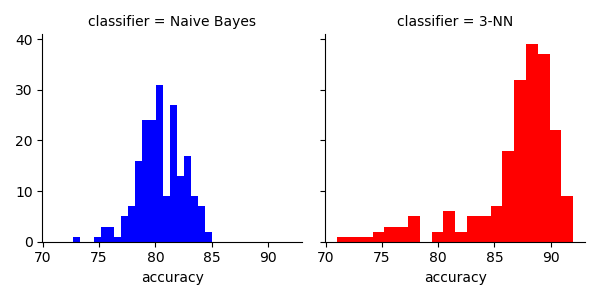
\includegraphics[width=0.9\textwidth]{nb_knn_comparison.png}
\caption{The accuracies of Na\"{i}ve Bayes and 3-NN classifiers, on 200
different training sets.}
\label{nb_knn_comparison}
\end{figure}

The result is shown in Figure~\ref{nb_knn_comparison}. It is very revealing.
First, notice that on average, the 3-NN classifier beats Na\"{i}ve Bayes. The
mean accuracies are:

\begin{Verbatim}[fontsize=\footnotesize,samepage=true,frame=single,framesep=3mm]
print("Naive Bayes: mean accuracy {:.2f}%.".format(nb_performances.mean()))
print("3-NN: mean accuracy {:.2f}%.".format(knn_performances.mean()))
\end{Verbatim}
\vspace{-.2in}

\begin{Verbatim}[fontsize=\footnotesize,samepage=true,frame=leftline,framesep=5mm,framerule=1mm]
Naive Bayes: mean accuracy 80.47%.
3-NN: mean accuracy 86.81%.
\end{Verbatim}

This tells us that 3-NN has \textbf{lower bias}, which is a good thing: good
enough for another 6\%-ish prediction accuracy, in fact.

The second thing to notice, though, is that the performance of 3-NN is more
variable. Its range is from 70-92, as opposed to Na\"{i}ve Bayes' 73-85. This
means that on some training sets, its performance is actually lower than the
worst of any of the Na\"{i}ve Bayes runs. The standard deviation bears this
out:

\begin{Verbatim}[fontsize=\footnotesize,samepage=true,frame=single,framesep=3mm]
print("Naive Bayes: standard deviation {:.2f}.".format(nb_performances.std()))
print("3-NN: standard deviation {:.2f}.".format(knn_performances.std()))
\end{Verbatim}
\vspace{-.2in}

\begin{Verbatim}[fontsize=\footnotesize,samepage=true,frame=leftline,framesep=5mm,framerule=1mm]
Naive Bayes: standard deviation 2.04.
3-NN: standard deviation 4.07.
\end{Verbatim}

\index{no free lunch@the ``no free lunch'' principle}

So 3-NN has \textbf{higher variance}, which is a bad thing. If we get unlucky
with our training set, we're going to have an inaccurate classifier. As I said,
there's no free lunch.

\bigskip

It's tempting to think that high variance isn't as bad as high bias. After all,
even though we might get unlucky, shouldn't we still choose the option with the
higher mean?

But the problem is that in real life, our training set and our new data are
almost never measured at the same time, and in exactly the same circumstances.
We collected data at some point in the past, train our classifier on it in the
present, and will run it to classify new data in the future. If the patterns in
the data fluctuate at all between past and future (as they invariably do), then
a high-variance classifier will ``lock on'' to those (obsolete) patterns in the
past and try to apply them to the future data. A low-variance classifier won't
make that mistake, since it's not as ambitious: it's settling for less precise,
but more generally applicable trends.


\subsection{Varying $k$}

Restricting our focus for the moment to just kNN classifiers, the question
arises as to the optimal value of $k$. It may or may not surprise you to learn
that there's no easy answer to this, and that it varies widely by data set and
in fact even by the training set chosen.

Here's some code to try all (odd) values of $k$ between 1 and 29. For each
value, it runs ten different trials and averages their performance, so that we
can smooth out the differences from particularly lucky or unlucky training sets:

\begin{Verbatim}[fontsize=\footnotesize,samepage=true,frame=single,framesep=3mm]
ks = np.array([])
performances = np.array([])

for k in range(1,30,2):
    for trial in range(10):
        ks = np.append(ks, k)
        performances = np.append(performances, kNN(s, k))

results = pd.DataFrame({'k':ks, 'performance':performances})
agg_results = results.groupby('k').performance.mean()
agg_results.plot(kind='line', color='red',ylim=(70,100))
\end{Verbatim}

The resulting plot is in Figure~\ref{fig:varyingK}. This Sith/Jedi data set is
simple enough that there aren't many really noticeable trends. Basically, as
long as $k$ is above 5 or so, we max out the performance. Only when $k=1$ or
$k=3$ do we see the too-high-variance problem come into play.

\begin{figure}[ht]
\centering
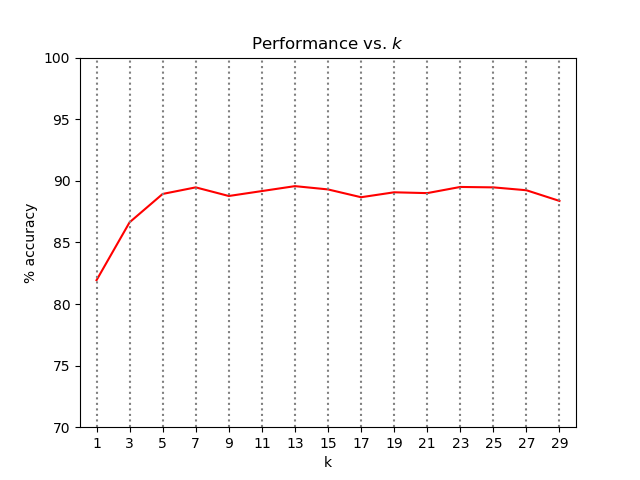
\includegraphics[width=0.9\textwidth]{varying_k.png}
\caption{The accuracy of a kNN classifier on the Sith/Jedi data, as we fiddle
with the number of nearest neighbors used.}
\label{fig:varyingK}
\end{figure}

Real-life data sets normally have more variation than this. Often, there's an
optimal range for $k$ that's quite a bit better than values outside that range,
and there's no surefire way to predict what that range will be until you try
it.

In general, though, the big picture is that \textit{as $k$ increases, the
classifier becomes lower-variance and higher-bias.} Can you see why? For low
values of $k$, we're picking the one (or three, or five, or ...) training
points that just happen to be nearest to our new data point. That's going to be
a lot different depending on which points happen to be in the training set. But
if $k$ is, say, 99, then no matter what training set we get, we're going to
classify most points the same. Like the simple ``just go based on lightsaber
color'' classifier described on p.~\pageref{simpleClassifierTable}, too many
different things would have to simultaneously change between training sets in
order for any different result.


\begin{figure}[ht]
\centering
\begin{Verbatim}[fontsize=\small,samepage=true,frame=single,framesep=3mm]
# Run Naive Bayes, and return the accuracy as a percentage.
def naive_bayes(s):
    train = s.sample(frac=.7)
    test = s.drop(train.index)

    oe = OrdinalEncoder()
    converted_features = oe.fit_transform(train.drop(['type'], axis=1))

    naive_bayes = CategoricalNB()
    naive_bayes.fit(converted_features, train.type)
    nb_predictions = naive_bayes.predict(
        oe.fit_transform(test.drop(['type'], axis=1)))
    return (nb_predictions == test.type).sum() / len(test) * 100


## Run kNN, and return the accuracy as a percentage.
def kNN(s, k):
    train = s.sample(frac=.7)
    test = s.drop(train.index)

    ohe = OneHotEncoder()
    one_hotted_features = ohe.fit_transform(train.drop(['type'], axis=1))

    knn = KNeighborsClassifier(n_neighbors=k)
    knn.fit(one_hotted_features, train.type)
    knn_predictions = knn.predict(
        ohe.fit_transform(test.drop(['type'], axis=1)))
    return (knn_predictions == test.type).sum() / len(test) * 100
\end{Verbatim}

\caption{Two functions, each of which chooses a random 70\% of a data set's
rows for training, runs a classifier on the remaining rows, and returns its
percent accuracy. Note that every time either of these functions is called, a
different answer will be returned, since a new training set will be chosen at
random.}
\label{comparisonCode}
\end{figure}

\section{``The curse of dimensionality''}
\label{sec:curse}

\index{curse@``the curse of dimensionality''}

A second key ML principle goes by the humorous name ``\textbf{the curse of
dimensionality}.'' It goes something like this. Suppose that in addition to
\texttt{height}, \texttt{demeanor}, \texttt{lightsaber}, and \texttt{face}, we
also have at our disposal many other features about Jedi \& Sith: their ages,
salaries, home planets, personality profiles, number of traffic tickets,
\textit{etc.} This is good news, right? It gives us more and more data to sift
through statistically and discover potential correlations with, right? What's
not to like?

\index{data sparsity}
\index{sparsity}

Yes, but there's a catch. It turns out that as we increase the number of
features more and more (or, put another way, as we increase the
``dimensionality'' of the problem from our original four dimensions to 5, 6, 7,
..., and up into the hundreds) we have a \textbf{data sparsity} problem. This
means there aren't enough training points to adequately cover all of this
ground.

In terms of kNN classifiers, you can think of it this way: effectively,
\textit{all} the points become far apart. We want to find the 3 (or 15, or 77)
``nearest neighbors,'' but when we have so many features (many of which will
turn out to be irrelevant for the problem), we find that \textit{any} two data
points will differ on a large number of them. Essentially, our noise swamps our
signal.

When we have tons of features, we need an enormous number of training samples
in order to guarantee that we have several samples with each combination of
values (or their ranges). In our original problem, we didn't need too much data
to ensure that we'd have at least a few \texttt{tall},
\texttt{green}-lightsabered, \texttt{menacing} individuals with a
\texttt{clean} face. But how many training points will we need before we have
several \texttt{tall}, \texttt{green}-lightsabered, \texttt{menacing},
38-year-old, extroverted, abstract-thinking individuals from Tatooine with 4
traffic tickets and a beard who earn 6,000 Galactic credits annually? Answer: a
lot. And if we don't have that many, a kNN classifier trained on all those
features is going to struggle trying to find ``people like this one'' in order
to make a prediction.

\index{feature selection}

The moral to the story is that we will often need to trim our set of features,
sometimes aggressively, if we have too many. It feels wasteful -- all this
great data on all these people, and we're throwing it away! -- but it's the
right thing to do. This process is called \textbf{feature selection}, and
we'll cover it more fully in the next chapter.
% FIX: actually add the feature selection chapter. (lesson 14 from 2019)

\medskip
In the meantime, here are three useful principles for avoiding the curse:

\begin{enumerate}

\item By far the most important thing to recognize is that if you have
additional features that are \textit{truly} correlated with the target -- and
don't simply repeat information contained in the features you already have --
it's okay to include them. Adding more stuff that actually contains useful
information for prediction isn't generally a problem. The problem is when you
add features that are largely \textit{noise}, since they will overwhelm the
truly significant features if there are too many of them.

\item A common rule of thumb is to make sure you have at least \textit{five}
training points for each combination of feature values. (In our Jedi example,
with three \texttt{height}s and three \texttt{lightsaber} values and two
values for the other features, this would imply a training set of at least $(3
\times 3 \times 2 \times 2) \times 5 = 180$ training points.)

\index{parametric model}

\item When the size of the training set becomes too small, use
\textbf{parametric} methods (like Na\"{i}ve Bayes or linear regression) rather
than instance-based methods (like kNN) because they suffer less from the curse.

\end{enumerate}


 
% TODO: talk about "percentage of variance explained," and point out that they
% don't add up to 100%.

\chapter{Feature selection}

\index{feature selection}
\index{curse@``the curse of dimensionality''}

The ``curse of dimensionality'' (p.~\pageref{sec:curse}) makes us inclined to
actually use fewer features in our classifier than we have at our disposal.
This is for two reasons:

\begin{itemize}
\itemsep.1em
\item Many of the available features are likely to be ``noisy,'' meaning they
are only loosely correlated with the target feature, if at all. Including
noisy features will make it more difficult for any classifier to separate the
wheat from the chaff: the features which truly are predictive will get drowned
out by those that merely clutter the picture.

\item Even for those features which do contain substantive, reliable
information about the target, it's not likely that they're all
\textit{independent} of each other. If (say) five of our twenty features each
furnished some unique and meaningful information about what the target label
is likely to be, that sounds great...but it's more likely that some (or even
all) of these five are correlated with each other, and hence contain
overlapping information. We'll get a better-performing classifier if we
avoid giving it redundant features that contain pesky noise to boot.

\end{itemize}

So how do we reduce the feature space? There are essentially three approaches:

\begin{enumerate}
\itemsep.1em

\index{subset selection}

\item \textbf{Subset selection}. We'll simply choose a subset of the original
features and use those ``as is'' (after normalizing them or one-hot-encoding
them, of course).

\index{shrinkage}
\index{regularization}

\item \textbf{Shrinkage} (a.k.a. ``\textbf{regularization}''). Especially
popular with linear models, we can essentially ``tone down'' some of the less
important features by shrinking their coefficients towards zero.

\item \textbf{Transforming the feature space}. In this case, we actually don't
use the \textit{original} features at all; instead, we form a set of
new features out of parts of the original features. This may sound weird --
especially since our new features don't have any obvious ``meaning''; they're
just combinations of some of the original ones -- but it can be very powerful
and informationally efficient.

\end{enumerate}

I'll say much more about the first of these, since the latter two require some
advanced math.

\section{Subset selection}

Let's say we have four features in our original data set (call them
$F_0,F_1,F_2, \textrm{and} F_3$, to stick with Python's numbering
convention.) As stated above, we may not want to actually use all four. So
which ones could we use?

It turns out we have $2^4$ (which is 16) choices of different feature sets to
use. They are:

\begin{compactitem}
\item all four of them
\item just $F_0,F_1$ and $F_2$
\item just $F_0,F_1$ and $F_3$
\item just $F_0$ and $F_1$
\item just $F_0,F_2$ and $F_3$
\item just $F_0$ and $F_2$
\item just $F_0$ and $F_3$
\item just $F_0$
\item just $F_1,F_2$ and $F_3$
\item just $F_1$ and $F_3$
\item just $F_1$ and $F_2$
\item just $F_1$
\item just $F_2$ and $F_3$
\item just $F_2$
\item just $F_3$
\item none of them (just use the prior)
\end{compactitem}

The way we get the number ``$2^4$'' is to reason as follows: ``each feature can
either be included, or excluded, in any feature set we choose. So for each of
the four features, there are two independent choices (either take it or leave
it) which leaves us with $2 \times 2 \times 2 \times 2$ different possible sets
of features.''

The one using all of the features is most likely to overfit, and the one using
none of them is most likely to underfit. Often the best-fitting classifier (on
new data! not the original training data) will be one of the intermediate
ones.

So...how do we find that best-fitting classifier then?

\subsection{Consider all subsets}

The obvious solution is to say ``we've identified all possible subsets of
features, let's try 'em!'' And indeed we can do this if the number of features
is modest. Train a classifier (whether Na\"{i}ve Bayes, kNN, or anything else)
using only the features in a given subset, compute the error rate, and then
choose the subset with the lowest error rate.

Figure~\ref{fig:allSubsetsCode} (p.~\pageref{fig:allSubsetsCode}) contains some
code that does just that (for Na\"{i}ve Bayes)\footnote{Notes: the
\texttt{is\_numeric\_dtype()} function distinguishes between numeric and
categorical variables, so we can normalize one and one-hot the other. Also, on
some versions of Pandas, you may have to call ``\texttt{.reshape(-1,1)}'' on
the value of ``\texttt{df[feature].values}'' in the \texttt{else} branch of the
\texttt{prepare\_this\_puppy()} method.} The \texttt{security\_cam2.csv} file
we're using here is the one from Chapter~\ref{ch:naiveBayes2}, with both
categorical and numerical features in it.

The output I got when I ran this was:

\begin{Verbatim}[fontsize=\small,samepage=true,frame=leftline,framesep=5mm,framerule=1mm]
        beard,height,lightsaber: 93.87
        beard,demeanor,height,lightsaber: 93.40
        beard,demeanor,lightsaber: 93.20
        beard,lightsaber: 90.00
        demeanor,height,lightsaber: 90.00
        height,lightsaber: 90.00
        demeanor,lightsaber: 90.00
        lightsaber: 90.00
        beard,demeanor,height: 85.80
        beard,height: 85.60
\end{Verbatim}

\index{OneHotEncoder@\texttt{OneHotEncoder}}
\index{fit\_transform@\texttt{fit\_transform()}}
\index{CategoricalNB@\texttt{CategoricalNB}}
\index{is\_numeric\_dtype@\texttt{is\_numeric\_dtype()}}
\index{dtype@\texttt{dtype}}
\index{spycam}
\index{security camera}
\index{security\_cam2@\texttt{security\_cam2.csv}}

\begin{figure}
\begin{Verbatim}[fontsize=\scriptsize,samepage=true,frame=single,framesep=3mm]
from sklearn.preprocessing import OneHotEncoder
from sklearn.naive_bayes import CategoricalNB
from pandas.api.types import is_numeric_dtype

w = pd.read_csv("security_cam2.csv")
train = w.sample(frac=.7)
test = w.drop(train.index)

# Given a DataFrame and a set of column headings to include, return a
# NumPy matrix with all these features prepared and concatenated.
# "Prepared" means: (1) for categorical variables, one-hot them, and
# (2) for numeric variables, compute their Z-scores.
def prepare_this_puppy(df, include):
   ohe = OneHotEncoder(sparse=False)
   prepared_features = []
   for feature in include:
      if is_numeric_dtype(df[feature].dtype):
         thing = df[feature]-df[feature].mean()/df[feature].std()
         prepared_features.append(np.array([thing.values]).transpose())
      else:
         prepared_features.append(ohe.fit_transform(
             df[feature].values.reshape(-1,1)))
   return np.concatenate(prepared_features, axis=1)

feature_sets = [ 'lightsaber,face,height,demeanor',
                 'lightsaber,face,height',
                 'lightsaber,face,demeanor',
                 'lightsaber,face',
                 'lightsaber,height,demeanor',
                 'lightsaber,height',
                 'lightsaber,demeanor',
                 'lightsaber',
                 'face,height,demeanor',
                 'face,height',
                 'face,demeanor',
                 'face',
                 'height,demeanor',
                 'height',
                 'demeanor' ]
scores = pd.Series()

for feature_set in feature_sets:
   train_features = prepare_this_puppy(train,feature_set.split(","))
   test_features = prepare_this_puppy(test,feature_set.split(","))
   naive_bayes = CategoricalNB()
   naive_bayes.fit(train_features,train.type.values)
   nb_predictions = naive_bayes.predict(test_features)
   scores[feature_set] = round(
      sum(nb_predictions == test.type)/len(test)*100,2)

scores = scores.sort_values(ascending=False)[:10]
for feature_set, score in scores.items():
   print("{}: {:.2f}".format(feature_set,score))
\end{Verbatim}
\caption{Trying \textit{all} possible feature subsets with Na\"{i}ve Bayes.}
\label{fig:allSubsetsCode}
\end{figure}


By a hair, the feature set that excludes \texttt{demeanor} but includes
everything else did the best, with 93.87\% accuracy. Right behind it was the
full feature set. (If we ran this multiple times, with different training set
choices, our results would vary somewhat.) This isn't too surprising, since in
this artificial data set, all of the features \textit{were} pretty indicative
of Jediness/Sithness, and they all \textit{were} fairly independent of each
other.

\subsection{Sadly...}

Now here's the deal. Although we might think we could declare victory with
this ``consider all the possible subsets and choose the best'' technique, it
turns out that except in very small cases, \textit{it's absolutely
impossible.} Consider: what if instead of four features, we had forty?
(Certainly not a large number of features by \textit{any} means.) We would
have had:
\begin{align*}
2^{40} = 1,099,511,627,776
\end{align*}
\vspace{-.2in}

or over a trillion different possible sets of features. Even if we could train
a \textit{thousand} different classifiers on our training data \textit{every
second}, here's how long it would take:

\vspace{-.2in}
\scriptsize
% the center environment that used to wrap this align* is gone: align* is a
% full-width centred display anyway, and in the tagged build a center block
% containing only display math leaves an unclosed text-unit structure
\begin{align*}
1,099,511,627,776 \times 
    \frac{1\ \textrm{second}}{1000\ \textrm{classifiers}} \times
    \frac{1\ \textrm{minute}}{60\ \textrm{seconds}} \times
    \frac{1\ \textrm{hour}}{60\ \textrm{minutes}} \times
    \frac{1\ \textrm{day}}{24\ \textrm{hours}} \times
    \frac{1\ \textrm{year}}{365\ \textrm{days}}\\
{\normalsize \textrm{\textbf{= 34.9\ years}\ !}}
\end{align*}
\normalsize
\smallskip

Ouch. You probably haven't even been alive for that long. And obviously the
situation gets worse the greater the number of features. If we had merely 100
features (also not an unreasonably large number at all), the universe will
have long since died of heat death by the time we're finished considering
subsets, even if we had every computer that had ever been made working
non-stop on the problem.

\section{``Greedy'' approaches}

\index{greedy (algorithm)}
\index{tree}
\index{decision tree}

So we have to find a way to choose a subset of features without considering
every different possibility. The most common way to do this is to use a
\textbf{greedy algorithm}. (You may remember this term from the first volume of
this series, when we talked about the ``greedy'' decision tree induction
algorithm.) A greedy algorithm is a procedure that finishes computing quickly
because it repeatedly takes shortcuts. More precisely, a greedy algorithm
always chooses \textit{the immediately best-looking option} and goes with it,
ignoring the fact that if it took more time and considered further ahead, it
might have made an ultimately better choice.

(To further illustrate a greedy algorithm: imagine a chess program that always
tried to take a piece if one was open to capture. It figures, ``hey, taking
the opponent's pieces is a good thing, and there's a piece sitting there
unprotected: why not take it?'' Obviously such an algorithm might play well
against a newbie, but against even a modestly sophisticated player it would
suck, since it would be easily lured into traps. Without being able to
consider the longer-term consequences of what it's doing, it would make many
decisions that looked good in the near-term but which would soon be revealed
as dumb.)

\subsection{Forward selection}

\index{forward selection}

The most common greedy algorithm used for feature selection is called
\textbf{forward selection}:

\definecolor{shadecolor}{rgb}{.84,.84,1}
\begin{shaded}
\vspace{-.2in}
\begin{center}
\textbf{Forward selection algorithm}
\end{center}
% blank line below is REQUIRED in the tagged build: a display block (center)
% directly followed by another (the list) leaves an unclosed text-unit structure

\begin{compactenum}
\small
\item Train $p$ different one-feature classifiers, where $p$ is the number of
features, and see how each one does. Choose as the winner the feature that
works the best in isolation.
\item Now, for each of the $p-1$ remaining features, train a classifier with
your original winner \textit{plus} the new one. Choose as the winner the
``best''\footnotemark\ \textit{two}-feature classifier.
\item Repeat this for each of the $p-2, p-3, p-4, \dots$ remaining features,
finding the ``best'' three-feature, four-feature, five-feature, $\dots$
classifier.
\item Your final answer is the best of the ``best.'' Out of the ``best''
one-feature, two-feature, \textit{etc.} classifiers, choose the one with the
best performance. This is the feature set you'll declare the winner.
\end{compactenum}
\end{shaded}

\footnotetext{I put ``best'' in quotes here because it may well not actually be
the best two-feature classifier out of all possible two-feature classifiers, as
we'll see.}

Two things are important to see here. First, you're training and considering a
\textit{vastly} smaller number of classifiers than you are in the ``best
subset'' approach we did previously. For the forty feature case, you'll be
considering:

\vspace{-.25in}
\begin{align*}
\textrm{forward selection}&: 40 + 39 + 38 + \dots + 1 = 780\ \textrm{classifiers}\\
\textrm{best subset}&: 2^{40} = 1,099,511,627,776\ \textrm{classifiers}\\
\end{align*}
\vspace{-.45in}

So the time it will take to do this has gone from 35 \textit{years} to .78
\textit{seconds}. Not bad.

The other thing to recognize is that we are \textit{not} by any means
guaranteed to get the best possible set of features this way. In fact, we
almost certainly won't. To see this, you have to realize that the feature that
looks the best of all in isolation might \textit{not} be one of the
\textit{pair} of features that works best as a pair. And this phenomenon
continues every iteration of our forward selection loop.

This can seem weird at first: if feature $F_{26}$ gives us the best
one-feature classifier of all forty, shouldn't feature $F_{26}$ plus another
one be the best \textit{two}-feature classifier? The answer is not
necessarily. Much of the reason why has to do with the overlap between
features -- recall that they will almost certainly contain redundant
information among them, and so if you knew from the outset that you wanted a
two-feature classifier, you might well choose $F_4$ and $F_{39}$ instead of
$F_{26}$, which was a great solo artist but didn't pair up as well with anyone
else.

\subsection{Backward selection}

\index{backward selection}

As you might have guessed, you can do this entire process ``in reverse,''
which is appropriately called \textbf{backward selection}:

\definecolor{shadecolor}{rgb}{.84,.84,1}
\begin{shaded}
\vspace{-.2in}
\begin{center}
\textbf{Backward selection algorithm}
\end{center}
% blank line below is REQUIRED in the tagged build: a display block (center)
% directly followed by another (the list) leaves an unclosed text-unit structure

\begin{compactenum}
\small
\item Start by including \textit{every} feature (instead of none of them).
\item Train $p$ different $p-1$-feature classifiers, each of which
\textit{leaves out} one feature. Choose as the winner the one with the
best performance.
\item Now, repeatedly leave out another feature, and choose as a winner the
best $p-2$-feature, $p-3$-feature, $p-4$-feature, $\dots$ classifier.
\item Your final answer is the best of the ``best.'' Out of the ``best''
$p-1$-feature, $p-2$-feature, \textit{etc.} classifiers, choose the one with
the best performance. This is the feature set you'll declare the winner.
\end{compactenum}
\end{shaded}

Backward selection has the same advantages and disadvantages as forward
selection. Unsurprisingly, it will ordinarily \textit{not} produce the same
``best'' feature set that forward selection does (nor that best-subset does).
Often data scientists perform both forward and backward selection and then
spend some time scrutinizing the feature sets each came up with to decide on
their final, best feature set.

\subsection{Evaluating classifier ``goodness''}

By the way, I repeatedly referred to ``best performance'' in the description
above. What does this mean in practice? 

\index{bias-variance trade-off}
\index{overfitting}
\index{wiggly@``wiggly'' classifiers}

From the bias-variance trade-off, we know that more complex (``wiggly'')
classifiers will tend to overfit a data set. Hence we can't blindly use
performance on a training set to choose between a four-feature classifier and a
five-feature classifier, because the five-feature one will \textit{almost
certainly win for the wrong reasons.} If it has more features to work with, it
has more flexibility, and hence will surely ``wiggle'' closer to the points it
trains on. This could be a blessing but also a curse, depending on whether it's
really picking up signal or locking on to noise.

There are two different ways of dealing with this problem in order to
``fairly'' compare classifiers of different complexities. I think of them as
the math-oriented and the computer-science-oriented ways:

\begin{compactitem}

\index{Mallows@Mallows' $C_p$}
\index{AIC (Akaike Information Criterion)}
\index{BIC (Bayesian Information Criterion)}
\index{adjusted@adjusted $R^2$}

% TODO: mention that usual R^2 is 1-RSS/TSS. Adjusted is a way of penalizing a
% more complicated model.

\item \textbf{The ``math-oriented'' way.} If you use the entire data set to
train on, you can still adjust for the complexity factor by \textit{penalizing}
more complex models in a principled way. The details are outside the scope of
this class, but I'll throw the following buzzterms at you so that if you see
them you'll know what category to file them under: \textbf{``Mallows' $C_p$''},
\textbf{AIC}, \textbf{BIC}, and \textbf{adjusted $R^2$}. All of these are ways
of taking a model's error rate and adjusting it in light of how complex that
model is, and therefore how likely it is to overfit.

\item \textbf{The ``computer-science-oriented'' way.} Just use a separate
training set and test set, drrr. Any overfitting that a complex model might do
will automatically be penalized since it will perform poorly on the data it was
not trained on.

\end{compactitem}

\section{Shrinkage}

\index{shrinkage}
\index{ridge regression}
\index{lasso regression}

For completeness, I briefly mention two other common methods of dealing with
the too-many-features problem. The first, most commonly used in linear
regression/classification, goes by the general term ``\textbf{shrinkage},'' and
its two most common variants are called \textbf{ridge regression} and
\textbf{lasso regression}. These can both be thought of as ways of ``partially
including'' features. Each of them has a parameter you can dial to control how
aggressively they will ``shrink'' coefficients to zero. This helps when some of
your features are correlated with others, since dialing down their influence
will prevent them from jointly dominating the prediction. The mathematics are
subtle, although one point worth mentioning is that with lasso, feature
coefficients can actually be reduced all the way to \textit{zero}, which
effectively eliminates them and performs a kind of feature selection as in the
previous section. (Ridge regression does not have this property.)

\section{Transforming the feature space}

\index{dimensionality reduction}
\index{linear algebra}
\index{PCA (Principal Components Analysis)}
\index{SVD (Singular Value Decomposition)}

Finally, one of the coolest approaches to reducing the feature space is to
\textit{transform it into a different set of dimensions}. This may sound
heady, and it is: it involves some linear algebra which you may know or learn
someday. But the basic idea is that the raw features themselves, as given in
the data set, may not be the most useful measurements of the data: perhaps
some \textit{combinations} of the features can give us more mileage. Instead
of height, age, salary, and work experience, perhaps we can take some
mathematical function of height-and-age, and another mathematical function of
salary-and-work-experience, and work with those two combined features instead.
(Often, the combined features will involve components of \textit{all} the
original features, not just in pairs as in this example.) The general term
\textbf{dimensionality reduction} is what to look for in this area, together
with specific techniques like \textbf{principal components analysis} (PCA) and
\textbf{singular value decomposition} (SVD). 

\chapter{Association Analysis}

\index{association analysis}
\index{machine learning (ML)}

Classification isn't the only machine learning task. Another one is called
\textbf{association analysis}, in which the goal isn't to predict the class of
new data items, but rather to determine which features of a data set have
``interesting'' relationships. Usually, ``interesting'' means ``correlated in a
way that can be taken advantage of.''

The principles of association analysis are used in fields as diverse as
bioinformatics, recommender systems, and cybersecurity intrusion detection.
Another common application is \textbf{market basket analysis}, in which it can
be employed to detect which sets of products tend to be bought together. This
information is useful, for instance, to retailers who seek optimal product
placement and effective marketing campaigns.

\section{Market basket analysis}
\index{market basket analysis}
\index{VIP card}
\index{MVP card}
\index{transaction}

All competitive grocery stores today keep track of their customers' purchases
as they check out. Even if they don't have a rewards program to lure customers
into getting a store-specific ``VIP card,'' they still know which sets of
products were bought together in a single trip to the store. Each such trip,
consisting of multiple products being purchased, is called a
\textbf{transaction}.

This type of association analysis relies on a huge table (\texttt{DataFrame})
of 1's and 0's. Each row is a transaction, and each column is a product the
store sells. A ``1'' in an entry indicates that \textit{at least one} of that
product was bought in that transaction. (Interestingly, quantities typically
aren't stored; just binary information about ``did this purchase contain at
least one of that item or not?'') Here's one such data set:

\begin{center}
\begin{tabular}{|c|c|c|c|c|c|}
\hline
diet\_soda & apples & beer & chips\_ahoy & diapers & cat\_food \\
\hline
0 & 1 & 0 & 0 & 0 & 0 \\
1 & 1 & 0 & 0 & 0 & 1 \\
1 & 1 & 1 & 0 & 1 & 0 \\
0 & 0 & 1 & 1 & 1 & 0 \\
1 & 1 & 0 & 1 & 1 & 0 \\
1 & 1 & 1 & 1 & 1 & 1 \\
0 & 0 & 0 & 0 & 0 & 1 \\
. & . & . & . & . & . \\
\hline
\end{tabular}
\end{center}

The first customer in this set apparently just ran into the store to grab a bag
of apples, while the second one bought some Diet Coke, an apple, and a couple
bags of cat food, \textit{etc.}

\bigskip
Now, some terms:
\vspace{-.15in}

\begin{itemize}
\itemsep.1em

\index{itemset}

\item \textbf{itemset}: An itemset is a group of one or more items. For
instance, ``\{apples,beer,cat\_food,chips\_ahoy\}'' is an itemset, as is
``\{diet\_soda\}''.

\index{support count}

\item \textbf{support count}: The support count for a given itemset is
\textit{the fraction of transactions in the entire data set that contain that
itemset.} In the sample data above, the support count for ``\{diet\_soda\}'' is
$\frac{4}{7} = .571$, since four out of the seven transactions contained diet
soda. The support count for ``\{apples,chips\_ahoy,diapers\}'' is just
$\frac{2}{7} = .286$.

\index{association rule}
\index{rule, association}
\index{antecedent}
\index{consequent}

\item \textbf{association rule}: An association rule is a statement of a
relationship between two itemsets. It looks like this: ``\{A,B\} $\Rightarrow$
\{C\},'' which means ``people who buy A and B tend to also buy C.'' The itemset
before the arrow is called the \textbf{antecedent} and the one after it is
called the \textbf{consequent}. Association
rules are general correlations, not hard-and-fast mandates. Their reliability
can be measured with the metrics below:

\vspace{-.15in}

\begin{itemize}

    \index{support}

    \item \textbf{support}: An association rule's ``support\footnote{Note that
    the term \textbf{support} properly applies to a rule, whereas the term
    \textbf{support \textit{count}} applies to an itemset. The \texttt{mlxtend}
    package calls them both ``support,'' though.}'' is the fraction
    of transactions in the data set that contain \textit{both} its antecedent
    \textit{and} its consequent. It's a measure of how widespread and
    applicable it is. The rule ``\{diet\_soda, apples\} $\Rightarrow$
    \{beer\}'' has a support of just $\frac{2}{7} = .286$ in the data set
    above. A rule's support is always between 0 and 1.

    \index{confidence}

    \item \textbf{confidence}: An association rule's ``confidence,'' on the
    other hand, is a measure of its reliability. It's \textit{the fraction of
    the times that it could apply where it's actually correct}. In terms of
    support, it's $\frac{\textrm{support(whole
    rule)}}{\textrm{support\_count(antecedent)}}$ The rule
    ``\{diet\_soda,apples\} $\Rightarrow$ \{beer\}'' has a support of
    $\frac{2}{4} = .5$ in the data set above, since out of the four times that
    diet soda and apples were purchased together, beer was also purchased in
    two of them. A rule's confidence is always between 0 and 1.

    \index{lift}

    \item \textbf{lift}: Finally, an association rule's ``lift'' is a numerical
    measure of how much predictive power it has. The key concept is that we
    want to know how likely the consequent is to be satisfied when the
    antecedent is satisfied \textit{relative to how likely the consequent is to
    be satisfied anyway.} Quantitatively, it's $\frac{\textrm{confidence(whole
    rule)}}{\textrm{support\_count(consequent)}}$. A rule's lift is always
    \textit{between 1 and $\infty$.} A lift of 1 means it's essentially
    useless: knowing the antecedent is true doesn't really make the consequent
    any more likely. \end{itemize}

\end{itemize}

\vspace{-.1in}

If we crunch all the numbers, we want to look for association rules with high
support, high confidence, and high lift. Which of those three end up being
the greatest priority depends somewhat on the application. If a rule doesn't
have high support, it doesn't come up much, so it may not be very useful. If
it doesn't have high confidence, then the trend it signifies isn't super
reliable, and we need to be aware of that. And if it doesn't have high lift,
then its antecedent doesn't tell us a whole lot that we didn't already know.

\vspace{-.1in}

\section{Implementation: the \texttt{mlxtend} library}

\index{conda install@``\texttt{conda install}'' command}
\index{mlxtend@\texttt{mlxtend} (package)}
\index{scikit-learn@\texttt{scikit-learn} (package)}
\index{Raschka, Sebastian}

Surprisingly, \texttt{scikit-learn} doesn't seem to have an association
analysis implementation out of the box. (At least, Stephen couldn't find one.)
There is one in the open source \texttt{mlxtend} library, though, by Sebastian
Raschka \& friends. You may need to run ``\texttt{conda install mlxtend}'' at
the command line for Spyder to access it.

\index{synthetic data set}
\index{association}
\index{prior (probability)}

\smallskip
Let's take it for a spin. First, we'll generate a synthetic data set with a
known association. We'll stock five items for sale in our pretend store, each
of which will have a different prior probability of being purchased (about 60\%
of all transactions will have bananas, 80\% will have pizza, \textit{etc.})
However, we'll ensure that in addition to 2,000 purely random ones, we'll have
a solid \textit{thousand} transactions with both bacon and eggs. This should
guarantee that ``\{bacon\} $\Rightarrow$ \{eggs\}'' comes out to be a
meaningful association.\footnote{``...and \{eggs\} $\Rightarrow$ \{bacon\} too,
right?'' you ask. Well, not necessarily, or at least not as strong: since 70\%
of the random transactions have eggs anyway, and only 10\% of them have bacon,
we're going to get a lot of bacon-less egg-full transactions, which will dial
down the confidence of that association. But let's wait and see what
\texttt{mlxtend} says.} Figure~\ref{fig:synthGroceries}
(p.~\pageref{fig:synthGroceries}) gives some code to synthesize such a data set.

\begin{figure}[ht]
\centering
\index{banana (fruit)}
\index{coffee}
\index{bacon}
\index{egg}
\index{pizza}
\begin{Verbatim}[fontsize=\footnotesize,frame=single,framesep=3mm]
eggs = []
bacon = []
bananas = []
pizza = []
coffee = []

for i in range(2000):
    eggs.append(np.random.choice([1,0],p=[.7,.3]))
    bacon.append(np.random.choice([1,0],p=[.1,.9]))
    bananas.append(np.random.choice([1,0],p=[.6,.4]))
    pizza.append(np.random.choice([1,0],p=[.8,.2]))
    coffee.append(np.random.choice([1,0],p=[.3,.7]))

for i in range(1000):
    eggs.append(1)
    bacon.append(1)
    bananas.append(np.random.choice([1,0],p=[.6,.4]))
    pizza.append(np.random.choice([1,0],p=[.8,.2]))
    coffee.append(np.random.choice([1,0],p=[.3,.7]))

transactions = pd.DataFrame({ 'eggs':eggs, 'bacon':bacon,
    'bananas':bananas, 'pizza':pizza, 'coffee':coffee})
\end{Verbatim}
\caption{Synthesizing a grocery shopping cart data set.}
\label{fig:synthGroceries}
\end{figure}

\bigskip

Okay, let's analyze. First, let's shuffle the \texttt{DataFrame}'s rows so
they're in a random order (not strictly necessary, but just on principle) and
then let \texttt{mlxtend} do its work:

\index{sample@\texttt{.sample()} (Pandas)}
\index{import@\texttt{import}}

\begin{Verbatim}[fontsize=\small,samepage=true,frame=single,framesep=3mm]
transactions = transactions.sample(frac=1)

from mlxtend.frequent_patterns import apriori
from mlxtend.frequent_patterns import association_rules

itemsets = apriori(transactions, min_support=0.1,
    use_colnames=True)
\end{Verbatim}

(Note that passing \texttt{frac=1} to the \texttt{.sample()} method says ``give
me \textit{all} the rows, please; but in a shuffled order.)

\index{apriori algorithm}
\index{min\_support@\texttt{min\_support}}

This code uses the so-called \textbf{apriori algorithm}. It computes the
support count \textit{only} for those itemsets that have a certain minimum
support level (in this case, \texttt{min\_support=0.1}). This is for simple
combinatorics reasons: if you think about it, the number of possible itemsets
is rather large if we have many columns. In fact, if we have $N$ columns, there
are $2^N$ different itemsets!\footnote{Sample numbers: if we have 100 different
items for sale in our store -- certainly not a very large number at all --
we'll have 1,267,650,600,228,229,401,496,703,205,376 different itemsets to
consider. This is far, far more than the number of atoms in the universe.} The
apriori algorithm is smart about not evaluating them all, because it uses an
easy trick: in order for an itemset to have greater than (say) .1 support
count, \textit{all of its subsets} must also have at least that much support.
This lets apriori whittle down greatly the number of itemsets it needs to
consider.

\bigskip
Let's print out the ten itemsets with the greatest support count:
\begin{Verbatim}[fontsize=\small,samepage=true,frame=single,framesep=3mm]
itemsets.sort_values('support',ascending=False).head(10)
\end{Verbatim}
\vspace{-.2in}

\begin{Verbatim}[fontsize=\small,samepage=true,frame=leftline,framesep=5mm,framerule=1mm]
               support                itemsets
              0.816000                  [eggs]
              0.801667                 [pizza]
              0.650667           [eggs, pizza]
              0.593333               [bananas]
              0.486000         [bananas, eggs]
              0.475333        [bananas, pizza]
              0.401667                 [bacon]
              0.387667  [bananas, eggs, pizza]
              0.380667           [bacon, eggs]
              0.316000          [bacon, pizza]
\end{Verbatim}

Not surprisingly, the one-item itemsets feature prominently in the list, with
eggs on the very top since not only did all of our second batch of 1000
transactions have eggs, but about 70\% of the others did as well.

\medskip

Now, let's generate (and compute stats on) all possible association rules
involving those item sets:

\begin{Verbatim}[fontsize=\footnotesize,samepage=true,frame=single,framesep=3mm]
rules = association_rules(itemsets)
print(rules.sort_values('confidence',ascending=False).head(10))
\end{Verbatim}
\vspace{-.2in}

\begin{Verbatim}[fontsize=\footnotesize,samepage=true,frame=leftline,framesep=2mm,framerule=1mm]
            antecedents consequents   support confidence     lift
        (bacon, coffee)      (eggs)   0.11900    0.95454  1.18626
         (bacon, pizza)      (eggs)   0.29966    0.94631  1.17603
                (bacon)      (eggs)   0.38100    0.94619  1.17588
       (bacon, bananas)      (eggs)   0.22500    0.94537  1.17486
(bacon, bananas, pizza)      (eggs)   0.17566    0.94275  1.17160
        (bacon, coffee)     (pizza)   0.10133    0.81283  1.02760
               (coffee)     (pizza)   0.24933    0.80777  1.02120
         (eggs, coffee)     (pizza)   0.20000    0.80645  1.01953
                (pizza)      (eggs)   0.63633    0.80446  0.99975
               (coffee)      (eggs)   0.24800    0.80345  0.99849
\end{Verbatim}

As expected, ``\{bacon\} $\Rightarrow$ \{eggs\}'' has a very high confidence
(and support, and lift), as do rules of the form ``\{bacon + various other
stuff\} $\Rightarrow$ \{eggs\}.'' Even in this synthetic case, however, the
lift values aren't all that high numerically, so don't expect them to be.

\section{Applying the knowledge}

\index{bacon}
\index{egg}

This is the point where the ML ends and the domain application begins. What
should a store do if armed with these statistics? In this case, we've learned
that \{bacon\} $\Rightarrow$ \{eggs\} is a good bet. So we might ask ourselves:
what product(s) that we're currently not selling very frequently (at least to
bacon \& egg lovers) would we like to sell more of? That choice of product will
have lots to do with inventory levels, the amount of markup we have on the
product (\textit{i.e.}, how much profit we make on it), and so forth.

\index{bagel}

Let's say we've identified a target product to market to these bacon \& egg
lovers: a new brand of bagels that's targeted specifically to big breakfast
eaters. It might make sense to position this item in our store somewhere
\textit{between} the aisles that bacon and eggs are sold on, so that every
person buying both bacon and eggs will have to walk past it. This is just one
simple example, but profit margins in grocery stores are so small that the
difference between booming and going out of business can rely precisely on many
micro-decisions like this, each inspired by a micro-insight from the data.
    

% TODO!!! Applications from Page's "The Model Thinker" chapter 10!

\chapter{``Special'' data types}

I'll end this book by alluding to a number of ``special'' types of data that
require somewhat different techniques to analyze that what we've learned so
far.

\index{time series}

One example is \textbf{time series} data, where observations are made at
regular, fixed points in time and one might be interested in identifying
overall trends (``stays at our hotel are going up!''), seasonal contributions
within those trends (``summers have more customers in general than winters
do''), and noise components that may obscure both effects (``we simply had a
bad year last year.'') A whole body of literature has arisen to treat time
series with specialized techniques.

\index{stemming}
\index{n-grams}
\index{free text / free-form text}
\index{natural language data}

Another example is \textbf{free-text} data (a.k.a. \textbf{free-form text},
a.k.a. \textbf{natural language data}) where the ``data'' is comprised of
actual written sentences in a language like English. This very unstructured
stream can be analyzed using a bevy of specialized techniques, from simple word
counts to sequences of words (``\textit{n-grams}'') to full parsing of
sentences. Often, techniques like \textbf{stemming} algorithms are used to
recognize that words like ``jump,'' ``jumped,'' and ``jumping'' all represent
the same basic concept. As with time series, the methods for working with
natural language are well studied, numerous, and form an entire subfield on
their own.

\index{geographic data}

Yet another example is \textbf{geographic data} (a.k.a. \textbf{geospatial
data}, a.k.a. \textbf{geodata}) used to represent points or areas on Earth.
Longitude and latitude, along with a set of transformational functions, can be
used to annotate data about events and perform computations to learn from them.

All of these topics (and others) each deserve their own course(s), and can only
be hinted at here.

\section{Graph-based data}

\index{network-based data}
\index{new kid@``new kid on the block''}

One other special data type which we'll spend some time on in this concluding
chapter is \textbf{graph-based} (or \textbf{network-based} data. It is rapidly
becoming one of the most important types of data in the world, especially in
view of the rise of our highly interconnected world (socially, culturally,
economically, \textit{etc.}) This type of data also a relatively ``new kid on
the block,'' which means that humankind is just now starting to get a handle on
how to analyze it. It's an exciting area to learn about because there's so much
(even relatively basic stuff) that's unknown and waiting to be discovered.

\index{graph}
\index{vertex (graph)}
\index{edge (graph)}

I'm using the word ``\textbf{graph}'' in a specialized sense here. It has
nothing to do with the x-y plot that word usually invokes in one's mind. It is
instead a special kind of data structure, or paradigm for organizing data.
Rather than rows in a table, a graph, or \textbf{network}, consists of
\textbf{vertices} (singular: \textbf{vertex}) connected by \textbf{edges}.
Here's an example:

\begin{center}
\label{first_example}
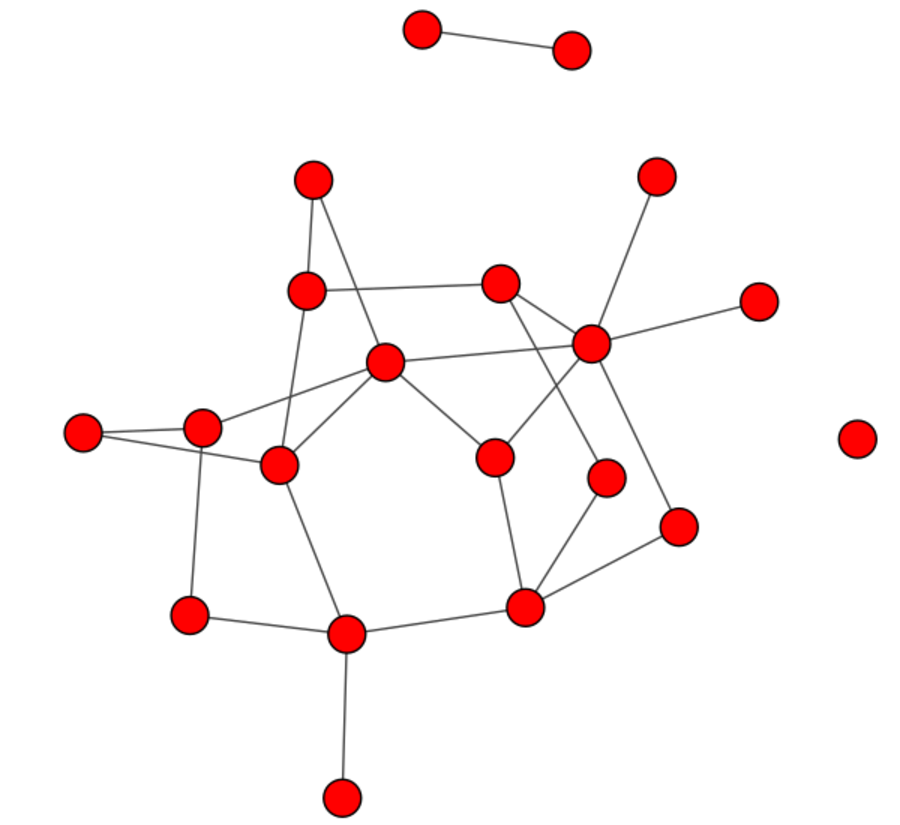
\includegraphics[width=0.7\textwidth]{first_example.pdf}
\end{center}

\index{node (graph)}
\index{link (graph)}
\index{arc (graph)}

The circles are the vertices (also sometimes called \textbf{nodes}) and the
lines are the edges (sometimes called \textbf{links} or \textbf{arcs}). This
basic structure can be used to describe innumerable kinds of things:

\begin{compactitem}
\itemsep.1em
\item People and the social ties between them.
\item Computers on a network and the connections that join them.
\item International banks and the transactions they've performed with one
another.
\item Physical locations and the routes/roads that connect them.
\item The pages on a particular website, and which ones link to which others.
\item Scholarly research papers and the citations they make of one another.
\item \textit{Etc.}
\end{compactitem}

\index{Aristotle}

Part of what makes graph-based data so important and powerful is this plethora
of different applications. Aristotle, in fact, thought that this
vertex-and-edge thing was so universal that essentially all the information we
might want to conceive could be reduced to, and represent with, this
structure.

\subsection{Graph terms}

A whole specialized vocabulary has sprung up for talking about graphs and
their properties. Here are just a few common terms and their meanings:

\begin{itemize}
\itemsep.1em

\index{order (of a graph)}
\index{size (of a graph)}

\item \textbf{order} and \textbf{size} -- Colloquially, researchers sometimes
refer to the number of vertices in a graph as its \textbf{order}, and the
number of its edges as its \textbf{size}. (The ratio of these quantities
becomes a subject of interest as well.)

\index{traversing (a graph)}

\item \textbf{to traverse} -- We use the verb ``\textbf{traverse}'' to mean
``follow a link from one node to another.'' This often comes up in the context
of searching for data in the graph, or finding a path through the graph with
certain features.

\index{directed graph}
\index{undirected graph}

\item \textbf{directed/undirected} -- In the graph above, vertices are
connected by simple lines. This is called an \textbf{undirected} graph, and
means that there is no intrinsic directionality to the edges: a pair of
vertices simply either is, or is not, joined by an edge. Sometimes, we care
about which ``way'' the edge goes -- for instance, if we represented a family
tree, and the edges indicated parent/child relationships. Saying ``Sam is the
daughter of Betty Lou'' is very different than saying ``Betty Lou is the
daughter of Sam.'' For this kind of graph, we will add arrowheads to the edges
to show this. We typically say that one can only traverse directed links in
the forwards direction (\textit{i.e.}, in the direction of the arrow).

\index{multigraph}
\index{self-loop}

\item a \textbf{simple graph} vs. a \textbf{multigraph} -- With most graphs,
there is at most one edge between any two pairs of vertices. (Either the
locations have a road between them or not, either the two people are friends
or they're not, \textit{etc.}) In some cases, though, we may allow
\textit{multiple} edges per vertex pair. Perhaps in our application we need to
know how \textit{many} roads connect two locations, or how many communications
were sent from person A to person B. Graphs that allow this are called
\textbf{multigraphs}. Multigraphs are also typically allowed to have
\textbf{self-loops} (an edge from a vertex to itself) which is not allowed in
a simple graph.

\index{attribute!of a graph edge or vertex}

\item \textbf{attributes} -- Both vertices and edges can be annotated with
special pieces of information called \textbf{attributes}. If vertices
represent people, perhaps we want to attach age or gender information to each
one. If edges represent communications between companies, maybe we want to
attach a date to each edge indicating when that communication took place. We
can depict attributes on the visual display (or not) through a variety of
means: text annotations, color/shape/size of the vertex, the thickness of the
line, and so on.

\index{weighted graph}

\item \textbf{weighted} graphs -- One particularly common type of \textbf{edge
attribute} is a number called the \textbf{weight} of the edge. This is often
depicted visually as the number positioned closely to the middle of the edge
itself. Typically this weight represents some sort of ``cost'' of ``using'' that
edge -- for instance, the distance (in feet) of the network cable between the
two computers, or the travel time (in minutes) of using the route from one
city to the other.

\index{degree (of a graph vertex)}
\index{in-degree}
\index{out-degree}

\item the \textbf{degree} (of a vertex) -- A vertex's ``\textbf{degree}'' is
simply the number of connections it has. In the diagram above, the bottom-most
node has degree 1, the one on the far right has degree 0, and the one at far
left has degree 2. For directed graphs, this notion expands to that of
``\textbf{in-degree}'' and ``\textbf{out-degree},'' which give the number of
incoming arrows and outgoing arrows, respectively.

\item the \textbf{degree sequence} (of a graph) -- If we take a census of the
degrees of all the vertices in a graph, and list them in descending order, we
get the \textbf{degree sequence} of the entire graph: The degree sequence of
the red graph on p.~\pageref{first_example}, as you can tediously verify, is:

\begin{center}
6, 5, 4, 4, 4, 3, 3, 3, 3, 2, 2, 2, 2, 2, 1, 1, 1, 1, 1, 0
\end{center}

\item the \textbf{degree distribution} (of a graph) -- A graph's
``\textbf{degree distribution}''  can be thought of as a histogram of its
degree sequence: how many nodes are there of degree 0? Of degree 5? Of degree
10? \textit{Etc.} The degree distro can tell us a lot about the overall
properties and structure of a large graph. Here's the one for our example:

\begin{center}
\index{degree distribution}
\label{degreeDistro}
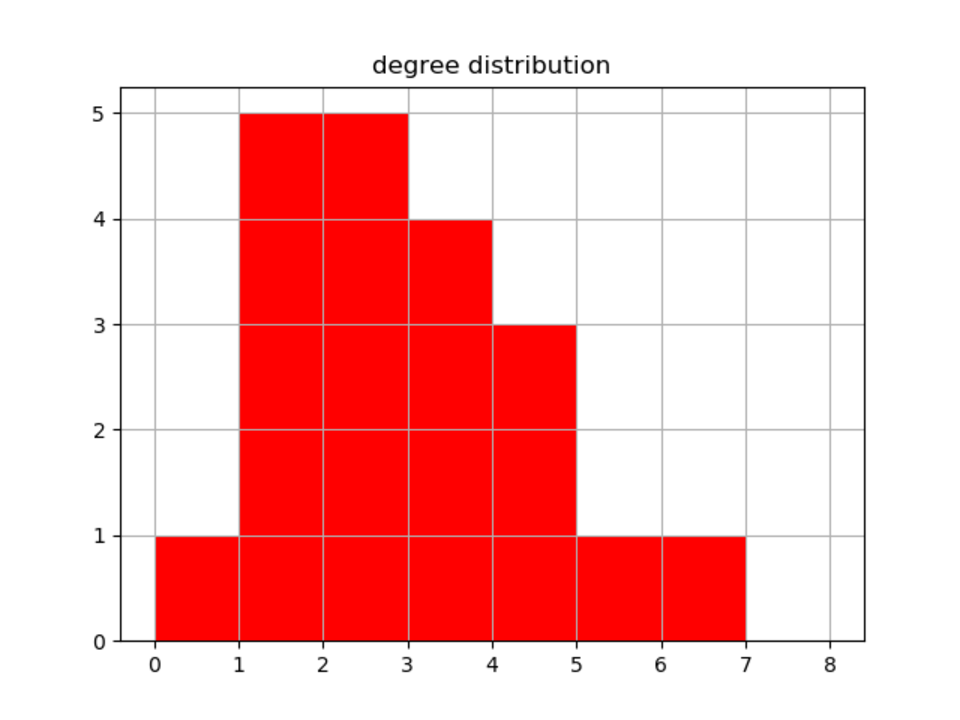
\includegraphics[width=0.7\textwidth]{degreeDistro.pdf}
\end{center}

\index{dyad}
\index{triad}
\index{clique} 
\index{triangle ($\triangle$)}

\item \textbf{dyads}, \textbf{triads}, and \textbf{cliques} -- The word
\textbf{dyad} is essentially just a synonym for \textbf{edge}. It means, ``any
pair of nodes that are completely connected together,'' where ``completely
connected'' means ``have an edge between them.'' This term may seem unnecessary
until you consider the related terms \textbf{triad} and \textbf{clique}. A
triad is a set of \textit{three} nodes which are \textit{completely} connected
to each other -- meaning, there is an edge between each pair of them. (Another
way to think of a triad is as a triangle $\triangle$.) ``Clique'' is the more
general word for ``some number of nodes, \textit{all of which} have an edge to
each of the others.'' We'll sometimes preface the word clique with a number,
and say ``this graph has a 5-clique'' or ``these eighteen vertices form an
18-clique.'' Note that a clique is a \textit{very} strong binding between the
vertices in a group -- they're totally inbred. Our red example on
p.~\pageref{first_example}, despite having a fair number of edges, has only a
single triad (can you find it?) and no cliques of higher order.

\item a \textbf{complete} graph -- a (or ``the'') complete graph of a certain
order is simply one that has every possible edge. A complete graph of order 4
will be of size 6, since there are 6 possible different pairs of vertices, and
hence 6 possible edges.

\index{subgraph}
\index{induced subgraph}
\index{clique}

\item \textbf{subgraph} -- a subgraph of a graph is simply one that has a
subset of its vertices and a subset of its edges. A clique, then, is a
\textit{complete subgraph} of a certain order. Sometimes we refer to an
\textbf{induced subgraph} of a graph: this is where we take (1) some subset of
the original graph's vertices as the vertices of the induced subgraph, and then
(2) all the edges in the original graph that connected vertices that we kept.
In this way, specifying only the vertex subset completely defines what the
induced subgraph will be.

\index{connected (graph)}
\index{reachable@``reachable'' vertex (graph)}

\item \textbf{connected} -- a graph is \textbf{connected} (sometimes called
``\textbf{fully connected},'' which means the same thing) if every vertex is
``reachable'' from every other vertex by traversing its edges. The red example
graph on p.~\pageref{first_example} is not connected, because there's a pair of
vertices at the top of the page that don't connect to anything else (and also
one lonely guy at the far right).

\index{directed graph}
\index{weakly connected (graph)}
\index{strongly connected (graph)}

Now what does ``connected'' mean for a \textit{directed} graph? There are two
notions: ``\textbf{strongly connected}'' and ``\textbf{weakly connected}.'' A
directed graph is strongly connected only if you can reach every vertex from
every other vertex only be traversing edges in the directions indicated. (No
going backwards on a one-way street.) It's weakly connected, on the other hand,
merely if it's connected once we \textit{ignore} the directionality of the
arrows.

\index{component (of a graph)}
\index{cluster (of a graph)}
\index{giant component@``giant component'' (graph)}

\item \textbf{component} -- a \textbf{component} (also sometimes confusingly
called a ``\textbf{cluster}'') of a graph is a connected subgraph. Very simple.
Every graph will contain one or more components, each of which is a sort of
island which can't be reached from the others. The red example on
p.~\pageref{first_example} has three components. A common term is
``\textbf{giant component}'' which is used to describe situations in which a
graph is not fully connected...but almost is. The big mass of nodes which are
all connected to each other is called the giant component to distinguish it
from the onsie-twosie others that aren't connected. Our example graph is of
just this type.

\index{community (graph)}

\item \textbf{community} -- in contrast to components, a \textbf{community} is
a much vaguer, more nuanced concept. Unlike component-ness, which has a razor
sharp criterion (all its nodes are reachable from each other, period) a
\textit{community} is an attempt to define a group of nodes that are
``reasonably'' connected to each other, at least when compared to their
connections with those outside the community.

\index{boys and girls}

Imagine a small social network for a high school class in which most girls
were friends with most of the other girls, most boys were friends with most of
the other boys, but there was also the occasional boy-girl friendship. We
could identify the set of girl nodes, and the set of boy nodes, as
``communities'' because they are relatively cohesive internally and relatively
decoupled from one another. Note that you can't ever really definitively
declare: ``such-and-such a set of nodes \textit{is} a community, whereas this
set definitely \textit{isn't}.'' It's more subtle than that. There's degrees of
``community-hood'' depending on how dense the connections are within and
outside the community.

\index{community detection}

The subfield of \textbf{community detection} is devoted to algorithms that
will identify such groups according to various criteria. It is a critical part
of social network analysis.

\index{cycle}

\item \textbf{cycle} -- in a graph, a \textbf{cycle} is a group of nodes that
are connected in a ring: you can start at one, traverse edges to the others,
and then return to where you started.

\end{itemize}

\subsection{Special kinds of graphs}

Certain patterns arise often enough to deserve their own names. Here are some
special kinds of graphs:
\begin{itemize}

% TODO: add figure with tree.

\index{tree}
\index{decision tree}
\index{parent (tree)}
\index{child (tree)}
\index{family tree}
\index{amoeba}
\index{asexually-reproducing organism}
\index{love letter}
\index{VP}
\index{crankshaft}
\index{piston assembly}
\index{cylinder head}
\index{My Computer@\texttt{My Computer}}
\index{C@\texttt{C:\textbackslash} drive}

\item \textbf{tree} -- A tree is a directed, connected graph with no cycles. (A
``family tree'' for an asexually-reproducing organism is a good example of
this, and often in fact we use the terms \textbf{parent} and \textbf{children}
to refer to the node that points to a particular vertex, and the nodes that
vertex points to, respectively.) You'll remember these from the
\textbf{decision tree} chapters in the first volume of this series: a decision
tree is in fact a tree.

A tree has the interesting property that exactly one of its nodes will have no
parent (we call it the ``\textbf{root}'' of the tree) and that there is
exactly one traversable path from the root to any other node in the graph.

Trees are used to represent a myriad of recursive hierarchical structures, such
as organizational charts (The President supervises the VPs, each VP supervises
Directors, each Director supervises Managers...), building assemblies (the
engine is composed of a piston assembly, a crankshaft, and a cylinder head,
which are each composed of...), information storage (the
\texttt{C:\textbackslash} drive contains \texttt{My Documents}, \texttt{My
Computer}, and \texttt{My Pictures}; \texttt{My Documents} contains
\texttt{DATA 101}, \texttt{DATA 219} and \texttt{love letters},...) and
countless more.

\index{Finlayson, Ian}
\index{DAG (directed, acyclic graph)}
\medskip

\item \textbf{DAG} -- Certain kinds of directed graphs, even if they're not
trees, must inherently be cycle-free to even make sense. For instance, the
graph of CPSC course prerequisites at
\url{http://ianfinlayson.net/misc/cpsc.png} (see below) must be cycle free
because the edges indicate required prerequisites, and if there were a cycle in
there...no one could ever graduate! These kinds of graphs are called
\textbf{DAGs} (``directed, acyclic graphs'') and are often used for managing
workflows in projects.

\begin{center}
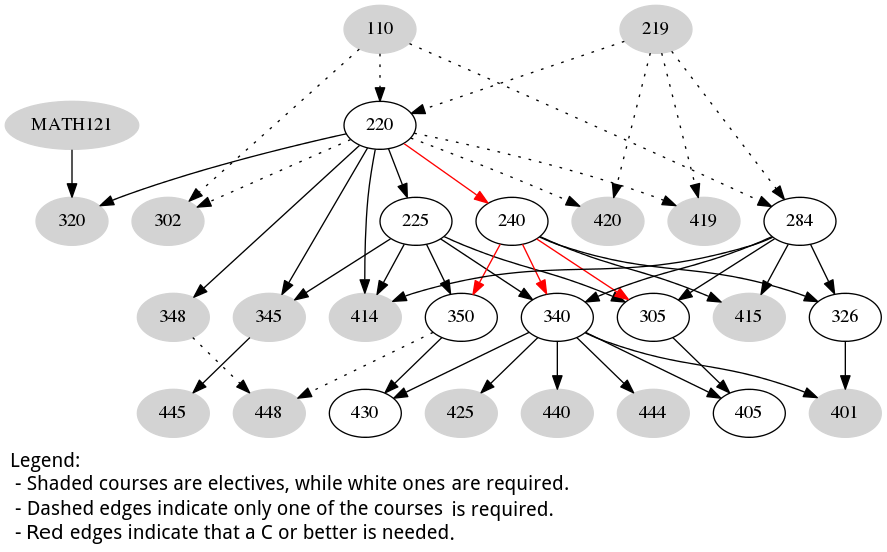
\includegraphics[width=0.7\textwidth]{courses.png}
\end{center}

\index{regular graph}

\item \textbf{regular graph} -- A graph is \textbf{\textit{d}-regular} if all
of its nodes have degree $d$. The graph below, for instance, is 3-regular
(check it out!)

\begin{center}
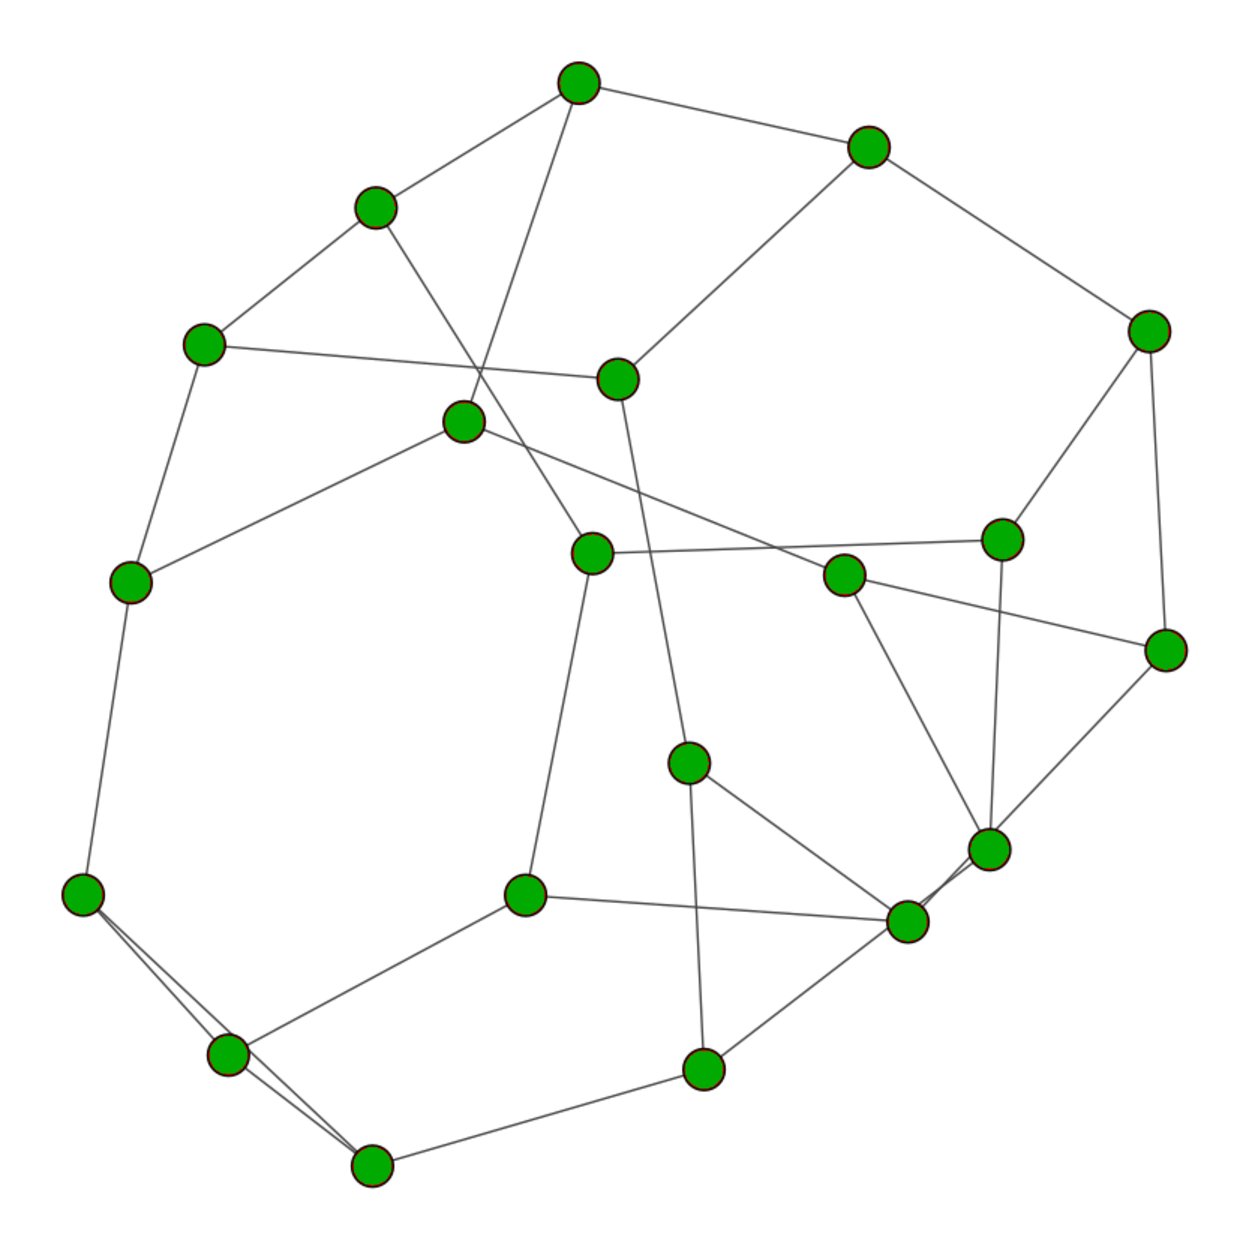
\includegraphics[width=0.5\textwidth]{regular.pdf}
\end{center}

\index{bipartite graph}
\index{heterosexual society}
\index{gender}
\index{recommender system}

\item \textbf{bipartite graph} -- A graph is \textbf{bipartite} if its vertices
can be split into two groups, and every edge \textit{only} joins a vertex from
one group with a vertex from the other. In a two-gender, completely
heterosexual society, the graph of dating relationships would be bipartite.
This kind of graph also comes up a lot in \textbf{recommender systems}: we have
two types of vertices: users, and (say) books. An edge between a user and a
book means that the user has purchased the book. (This is clearly bipartite,
because users never purchase each other, and neither do books.)

Bipartite graphs can be drawn with two rows of vertices, one of each type. All
the edges run across the middle.

\begin{center}
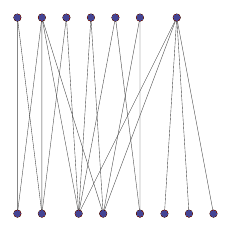
\includegraphics[width=0.4\textwidth]{bipartite.png}
\end{center}

\end{itemize}


\subsection{Representations}

\index{igraph@\texttt{igraph} (package)}
\index{Cs\'{a}rdi, G\'{a}bor}

When we use a graph package like \texttt{igraph}, by G\'{a}bor Cs\'{a}rdi, we
can ignore details about \textit{how} the graph we're working with is
represented under the hood. (Hint: it's not a bunch of circles and lines.)
However, there will be times when we need to retrieve, modify, or manipulate
one or more of these representations, so let's learn what they are.

\subsubsection{Edge list}

\index{edge list}
\index{CSV file}

To a data scientist, perhaps the most straightforward way to represent a graph
is via an \textbf{edge list}, which is very much like a CSV file or
\texttt{DataFrame}. Each line gives two vertex names or IDs, which are
connected by an edge.

\pagebreak
\begin{multicols}{2}
\begin{center}
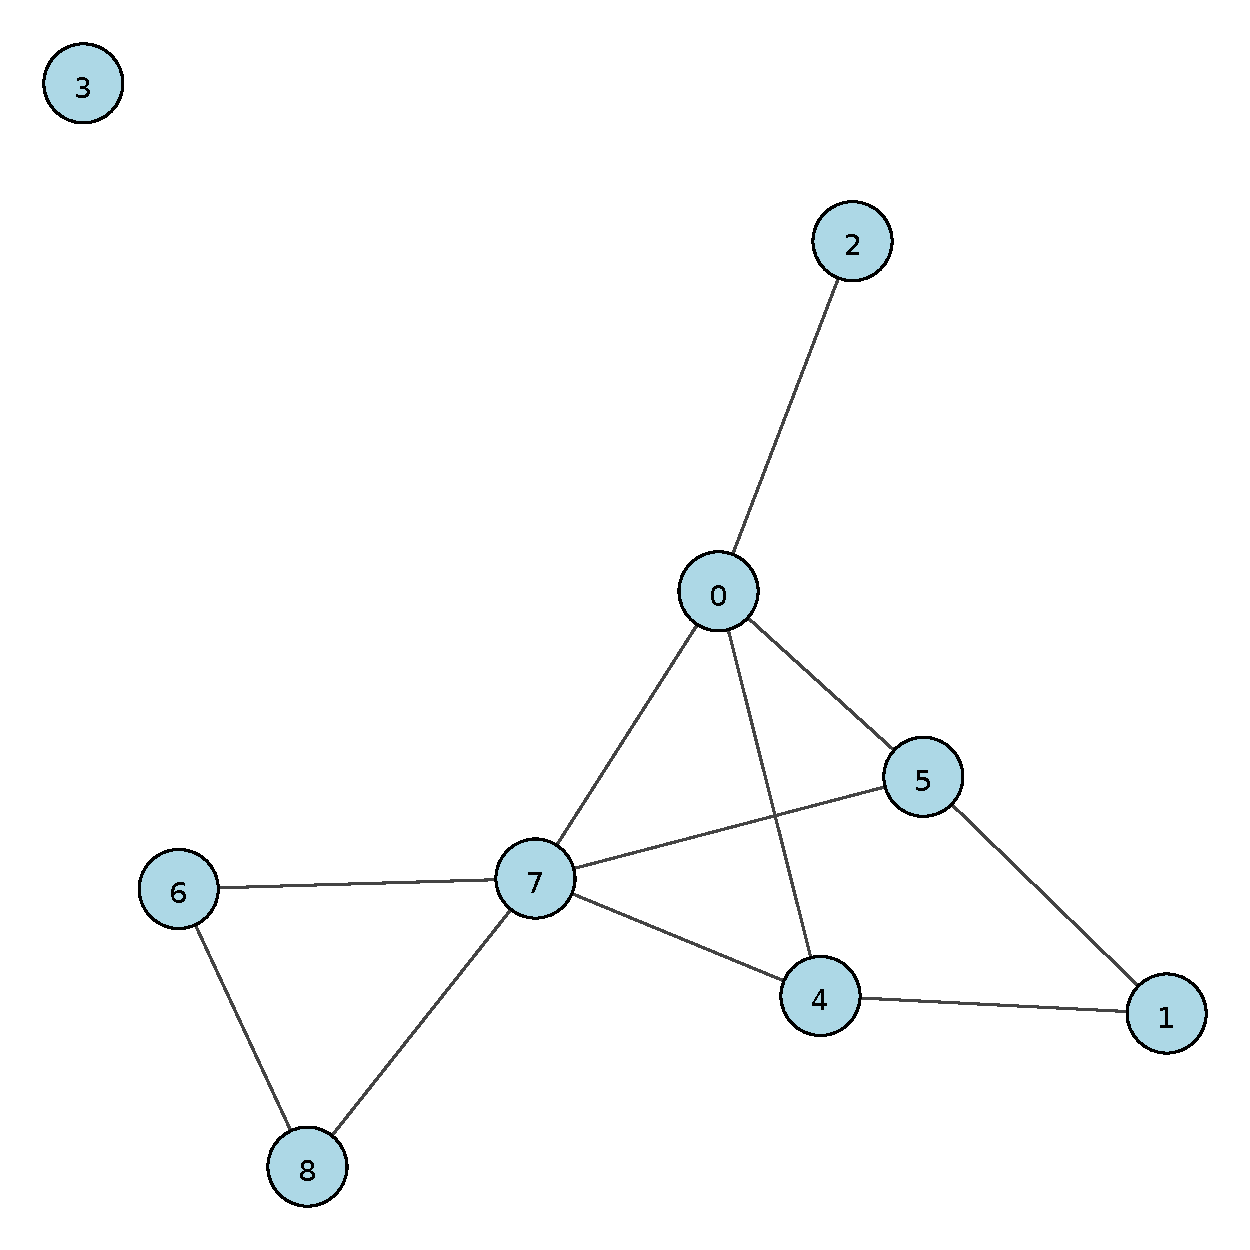
\includegraphics[width=0.48\textwidth]{second_example.pdf}
\end{center}
\columnbreak
  

Edge list:
\vspace{-.15in}
\begin{Verbatim}[fontsize=\small,samepage=true,frame=none]
      0,2
      0,4
      1,4
      0,5
      1,5
      0,7
      4,7
      5,7
      6,7
      6,8
      7,8
\end{Verbatim}
\end{multicols}

\index{directed graph}
\index{undirected graph}

For a directed graph, the order of entries within a line would matter, of
course, but for an undirected graph, it doesn't.

\subsubsection{Adjacency matrix}

\index{adjacency matrix}
\index{matrix}

A graph's \textbf{adjacency matrix} is used in lots of different analysis
techniques. It's simply a matrix (two-dimensional array) where every row (and
column) corresponds to one vertex. A ``1'' in an entry $(i,j)$ means ``yes,
vertex $i$ and vertex $j$ are connected.'' Otherwise, they're not.

\begin{multicols}{2}
\begin{center}
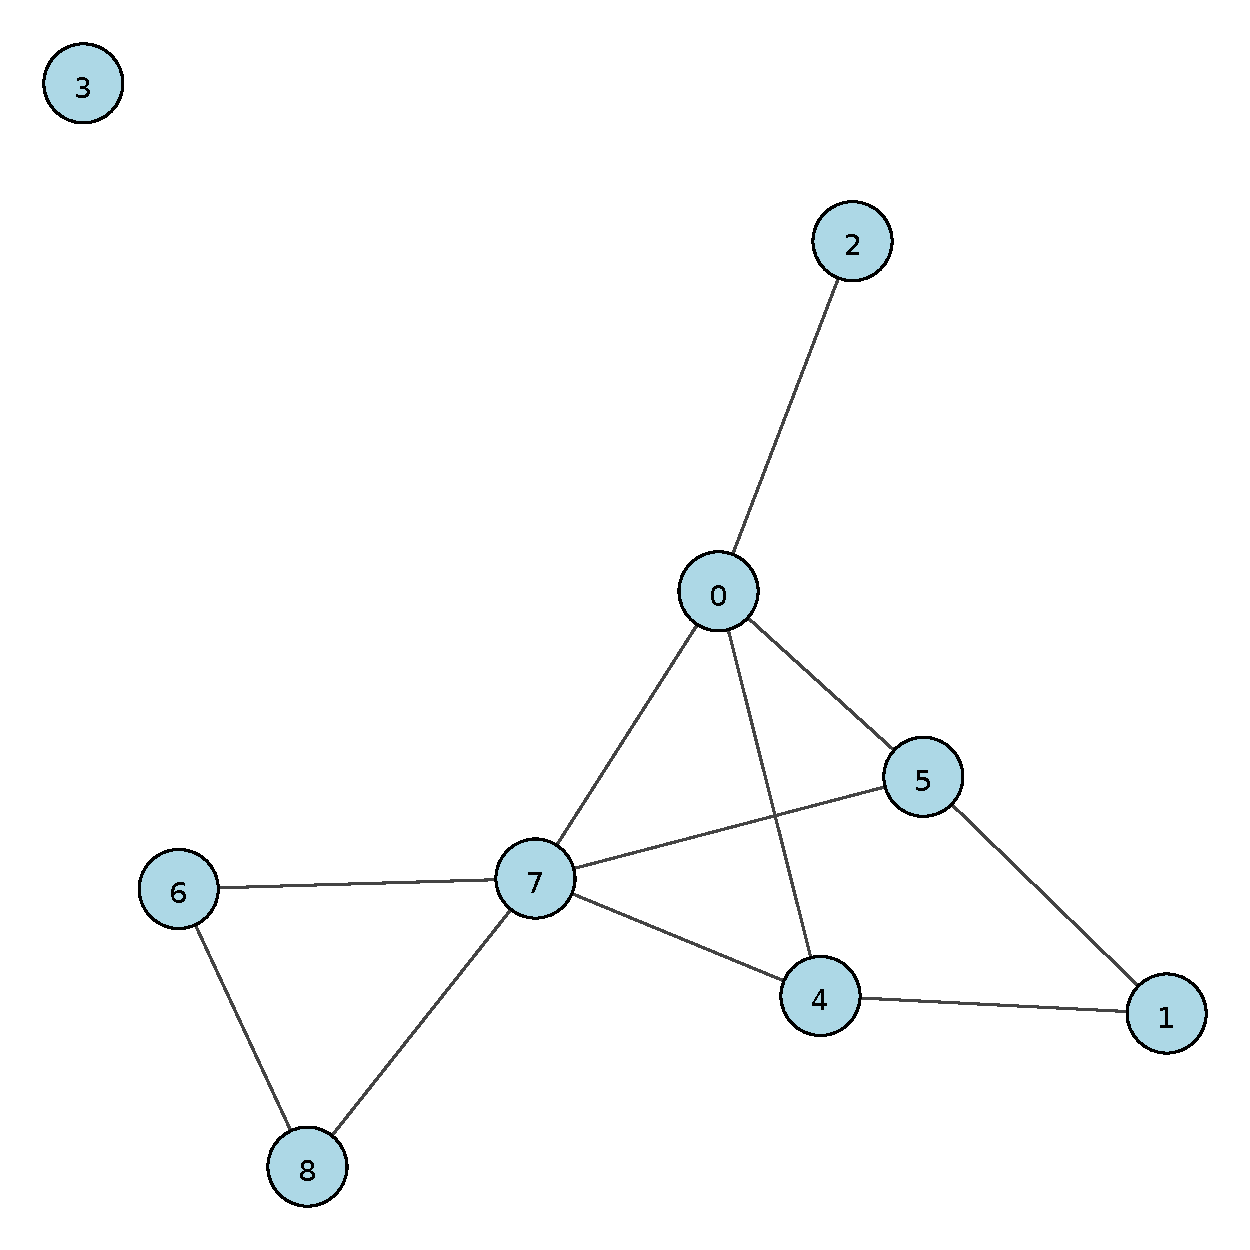
\includegraphics[width=0.48\textwidth]{second_example.pdf}
\end{center}
\columnbreak
Adjacency matrix:
\vspace{-.15in}
\begin{align*}
\begin{bmatrix}
  0 & 0 & 1 & 0 & 1 & 1 & 0 & 1 & 0 \\
  0 & 0 & 0 & 0 & 1 & 1 & 0 & 0 & 0 \\
  1 & 0 & 0 & 0 & 0 & 0 & 0 & 0 & 0 \\
  0 & 0 & 0 & 0 & 0 & 0 & 0 & 0 & 0 \\
  1 & 1 & 0 & 0 & 0 & 0 & 0 & 1 & 0 \\
  1 & 1 & 0 & 0 & 0 & 0 & 0 & 1 & 0 \\
  0 & 0 & 0 & 0 & 0 & 0 & 0 & 1 & 1 \\
  1 & 0 & 0 & 0 & 1 & 1 & 1 & 0 & 1 \\
  0 & 0 & 0 & 0 & 0 & 0 & 1 & 1 & 0 \\
\end{bmatrix}
\end{align*}
\end{multicols}

\index{directed graph}
\index{undirected graph}
\index{symmetric matrix}
\index{sparse matrix}

Note how for an undirected graph (as we have here) the adjacency matrix will
be \textbf{symmetric}, \textit{i.e.}, a mirror image across the main
(upper-left-to-lower-right) diagonal. Note also that for a high-order but
relatively low-size graph, the adjacency matrix will be \textit{huge} (and
``\textbf{sparse}'': mostly zeros), much larger than it needs to be.

\subsubsection{Adjacency list}

\index{adjacency list}

A much more compact version of the adjacency matrix is the \textbf{adjacency
list}, which addresses the sparsity problem. Instead of a big $n\times n$
matrix with mostly zeroes, the adjacency list only gives us, for each vertex,
\textit{a list of the other vertices it connects to}. It looks like this:

\begin{multicols}{2}
\begin{center}
\label{lightblueGraph}
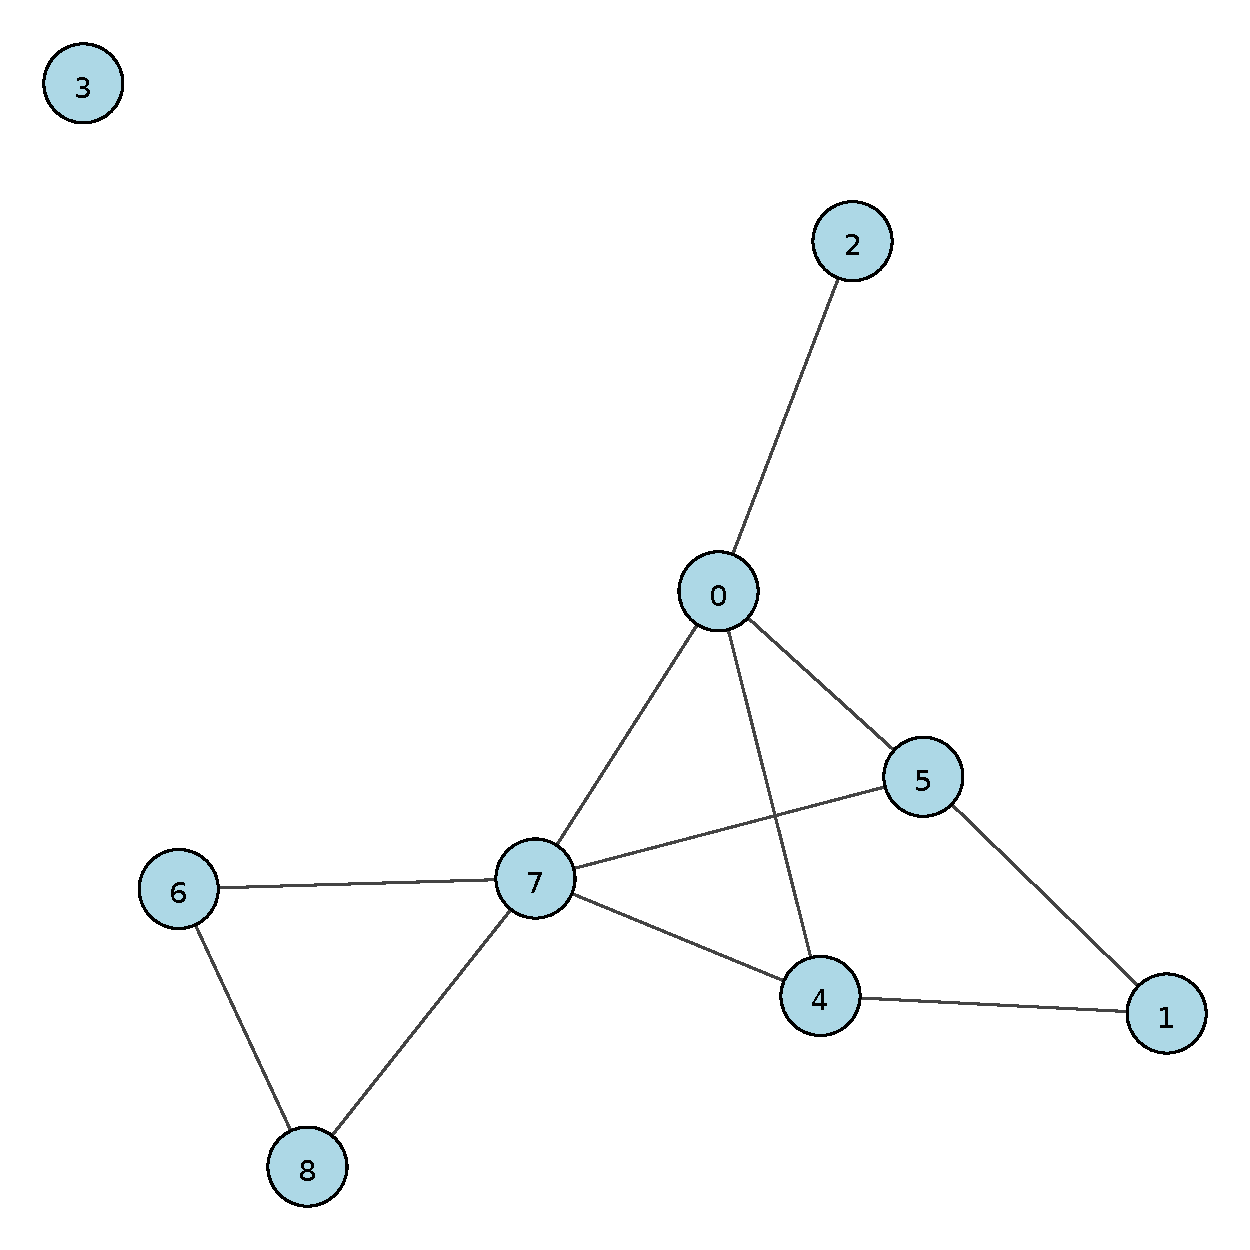
\includegraphics[width=0.48\textwidth]{second_example.pdf}
\end{center}
\columnbreak
Adjacency list:
\begin{Verbatim}[fontsize=\small,samepage=true,frame=none]
  0: [2, 4, 5, 7]
  1: [4, 5]
  2: [0]
  3: []
  4: [0, 1, 7]
  5: [0, 1, 7]
  6: [7, 8]
  7: [0, 4, 5, 6, 8]
  8: [6, 7]
\end{Verbatim}
\end{multicols}


\subsection{Descriptive measures}

Graphs are extremely expressive, but for that reason they're hard to get your
head around. If you look at a small graph (order 10, say), you can stare at it
long enough to figure out what the structure is: who's connected to whom,
where the cliques are, what the components are, and so on. But for anything
bigger, it's a maze. Looking at a two-dimensional representation doesn't
reveal much about the graph's inner properties. And it turns out that graphs
have many interesting inner properties that help explain its behavior in the
real world.

\index{degree distribution}

We've already seen one example of this, with the \textbf{degree distribution}
(p.~\pageref{degreeDistro}). This shows us, generally speaking, how many
high-connected and low-connected nodes we have, which may imply many things
depending on the domain.

\subsubsection{Clustering coefficient}

\index{clustering coefficient}
\index{transitivity}
\index{friend-of-a-friend}
\index{chevron ($\wedge$)}
\index{$\wedge$ (chevron)}
\index{triangle ($\triangle$)}

Another variable of interest is the \textbf{clustering coefficient}, also
sometimes called the \textbf{transitivity}, of a graph. It measures how often
it's true that friends-of-a-friend are also friends. If we define a ``chevron''
($\wedge$) as two nodes sharing a neighbor (\textit{i.e.}, vertex A is
connected to B, and B is connected to C), the transitivity tells us what
fraction of the time this is a complete triangle ($\triangle$) (\textit{i.e.},
how likely it is that A is connected to C). This tells us something about how
tightly clustered the graph is: are people wrapped up in tight-knit balls, or
are their relationships more spread out throughout the society? (The
transitivity of the light-blue graph on p.\pageref{lightblueGraph} is .36,
whereas the original red one on p.\pageref{first_example} was only .2.)

\subsubsection{Centrality measures}

\index{centrality measure}

A question that often arises in graphs is: which nodes are the most
\textbf{central}? By ``central'' we don't mean ``drawn near the center of the
page,'' since that is solely dependent on the layout algorithm, not the graph
structure. What, then, does ``central'' mean?

\bigskip
\index{closeness centrality}
\index{farness@``farness''}

One measure is called \textbf{closeness centrality}. For a given node $x$,
suppose we calculate \textit{the sum of the length of the shortest paths
between $x$ and every other node.} This is called the ``\textbf{farness},'' and
will obviously be higher for nodes that are very far away from at least some
others. It will presumably be the lowest for nodes that are most centrally
located, since they are not hugely far from \textit{any} of the other nodes.


If we take the reciprocal of the farness, we get the ``\textbf{closeness},''
and often we normalize this by multiplying by the order of the graph (so we
can compare closeness values between graphs of different sizes.) The final
formula for the closeness centrality of a node $x$, then, is:
\begin{align*}
c_{\textrm{closeness}}(x) = \frac{N}{\sum_{v \in V} \textrm{dist(v,x)}}
\end{align*}
\index{geodesic distance}
where $N$ is the order of the graph, $V$ are the vertices in the graph, and
``dist($a,b$)'' is the shortest distance\footnote{Also sometimes called the
``\textbf{geodesic distance}'' just to be confusing.} between two nodes $a$ and $b$.

By this measure, the most central vertex in the light-blue graph is 7 (with a
$c_{\textrm{closeness}}$ of .444), followed by 0, 5, and 4. The ``least
central'' is node 3, with a measly .111.

\bigskip

A different way to think about centrality is in terms of information flow.
Suppose these vertices are actors in a social network. Which ones are most
crucial to a piece of news finding its way around to everyone? 

\index{betweenness centrality}

One way to measure this is with \textbf{betweenness centrality}. For a given
node $x$, we ask, ``of all the pairs of vertices $a$ and $b$, how often is $x$
on the \textit{shortest} path from $a$ to $b$?'' If information is to travel
from $a$ to $b$, it's probably most likely (though not certain) that it will
travel along the shortest path between those two nodes. So if $x$ is on a lot
of such paths, it means it will be a common conduit of information exchange
between others. We define this mathematically as follows:
\begin{align*}
c_{\textrm{betweenness}}(x) = \sum_{a,b\ \in\ V} \frac{\sigma(a,b\ |\ x)}{\sigma(a,b)}
\end{align*}

where the notation ``$\sigma(a,b)$'' means ``the number of shortest paths from
$a$ to $b$'' (there could be more than one of these, in case of a tie), and
where the notation ``$\sigma(a,b\ |\ x)$'' means ``the number of shortest paths
from $a$ to $b$ \textit{which pass through $x$}.''\footnote{Sometimes, we
normalize this by dividing by $(N-1)(N-2)$, to get it to be a number between 0
and 1 like the closeness centrality is.} The larger this number is, the
greater the chance that $x$ will participate in an exchange of information
between any two nodes.


Perhaps not surprisingly, for the light-blue case the same nodes are central
by both these measures. Node 7 has a (normalized; see footnote) betweenness
centrality of .184, followed by nodes 0, 5, and 4. One difference is between
nodes 1 and 8: $c_{\textrm{closeness}}(8)$ is higher than
$c_{\textrm{closeness}}(1)$ ($.348 > .333$), but $c_{\textrm{betweenness}}(1)$
is higher than $c_{\textrm{betweenness}}(8)$ ($.333 > 0$). This is because
although 8 is a bit closer to the heart of the action, he's not on
\textit{anyone's} shortest path to anyone else. (There's nobody better than
node 1, meanwhile, for getting info from 4 to 5.) Therefore, in terms of
information passing purposes, he's kind of useless.


\bigskip

\index{linear algebra}
\index{PageRank algorithm}
\index{eigenvectors}
\index{adjacency matrix}

Finally, for those who have linear algebra in their arsenal, there are various
ways of using \textbf{eigenvectors} of the adjacency matrix to measure
centrality. One of these algorithms is called \textbf{PageRank}, which you may
be familiar with since it made Google famous and the number one search engine
in the world. The idea is that the more central \textit{your neighbors} are,
the more central you're likely to be. (In terms of playground drama: a popular
person is not so much one with a lot of friends, but rather one with a lot of
\textit{popular} friends.)

\index{igraph@\texttt{igraph} (package)}

The math involved is beyond the scope of this course, but if you've had some
matrix algebra it's not too hard, and of course \texttt{igraph} can do the
heavy lifting for us.

% TODO: Star Wars graphs!

\section{Conclusion}

This has been nothing but a whirlwind tour to give you a taste of what graphs
are and why they're important. As I mentioned, they're quite possibly the most
important type of data in our new ultra-networked century, and currently
they're not very well understood. They deserve an entire course (or two!) in
their own right, and I hope to teach one someday!
         

\backmatter
\printindex

% The Blurb-only \shipout\null padding pages are deliberately omitted here:
% they produce untagged blank pages. Keep them in the print build only.

\end{document}